% Judul dokumen
\title{Buku Tugas Akhir ITS}
\author{Dhiyya'ul Haq, Ikhwanul Abiyu}

% Pengaturan ukuran teks dan bentuk halaman dua sisi
\documentclass[12pt,twoside]{report}

% Pengaturan ukuran halaman dan margin
\usepackage[a4paper,top=30mm,left=30mm,right=20mm,bottom=25mm]{geometry}

% Pengaturan ukuran spasi
\usepackage[singlespacing]{setspace}

% Pengaturan detail pada file PDF
\usepackage[pdfauthor={\@author},bookmarksnumbered,pdfborder={0 0 0}]{hyperref}

% Pengaturan jenis karakter
\usepackage[utf8]{inputenc}

% Pengaturan pewarnaan
\usepackage[table,xcdraw]{xcolor}

% Pengaturan kutipan artikel
\usepackage[style=ieee, backend=biber]{biblatex}

% Package lainnya
\usepackage{changepage}
\usepackage{enumitem}
\usepackage{eso-pic}
\usepackage{txfonts} % Font times
\usepackage{etoolbox}
\usepackage{graphicx}
\usepackage{lipsum}
\usepackage{caption}
\usepackage{longtable}
\usepackage{tabularx}
\usepackage{wrapfig}
\usepackage{float}
\usepackage{array} % Add this line in the preamble

\captionsetup[longtable]{
  width=.9\textwidth, % Adjust the width to .9 of the text width or as needed
}

% Definisi untuk "Hati ini sengaja dikosongkan"
\patchcmd{\cleardoublepage}{\hbox{}}{
  \thispagestyle{empty}
  \vspace*{\fill}
  \begin{center}\textit{[Halaman ini sengaja dikosongkan]}\end{center}
  \vfill}{}{}

% Pengaturan penomoran halaman
\usepackage{fancyhdr}
\fancyhf{}
\renewcommand{\headrulewidth}{0pt}
\pagestyle{fancy}
\fancyfoot[LE,RO]{\thepage}
\patchcmd{\chapter}{plain}{fancy}{}{}
\patchcmd{\chapter}{empty}{plain}{}{}

% Command untuk bulan
\newcommand{\MONTH}{%
  \ifcase\the\month
  \or Januari% 1
  \or Februari% 2
  \or Maret% 3
  \or April% 4
  \or Mei% 5
  \or Juni% 6
  \or Juli% 7
  \or Agustus% 8
  \or September% 9
  \or Oktober% 10
  \or November% 11
  \or Desember% 12
  \fi}
\newcommand{\ENGMONTH}{%
  \ifcase\the\month
  \or January% 1
  \or February% 2
  \or March% 3
  \or April% 4
  \or May% 5
  \or June% 6
  \or July% 7
  \or August% 8
  \or September% 9
  \or October% 10
  \or November% 11
  \or December% 12
  \fi}

% Pengaturan format judul bab
\usepackage{titlesec}
\titleformat{\chapter}[display]{\bfseries\Large}{BAB \centering\Roman{chapter}}{0ex}{\vspace{0ex}\centering}
\titleformat{\section}{\bfseries\large}{\MakeUppercase{\thesection}}{1ex}{\vspace{1ex}}
\titleformat{\subsection}{\bfseries\large}{\MakeUppercase{\thesubsection}}{1ex}{}
\titleformat{\subsubsection}{\bfseries\large}{\MakeUppercase{\thesubsubsection}}{1ex}{}
\titlespacing{\chapter}{0ex}{0ex}{4ex}
\titlespacing{\section}{0ex}{1ex}{0ex}
\titlespacing{\subsection}{0ex}{0.5ex}{0ex}
\titlespacing{\subsubsection}{0ex}{0.5ex}{0ex}
\setcounter{secnumdepth}{3} % Untuk memberi penomoran pada \subsubsection

% Atur variabel berikut sesuai namanya

% nama
\newcommand{\name}{Ikhwanul Abiyu Dhiyya'ul Haq}
\newcommand{\authorname}{Dhiyya'ul Haq, Ikhwanul Abiyu}
\newcommand{\nickname}{Ikhwan}
\newcommand{\advisor}{Dr. Arief Kurniawan, S.T., M.T.}
\newcommand{\coadvisor}{-}
\newcommand{\examinerone}{-}
\newcommand{\examinertwo}{-}
\newcommand{\examinerthree}{-}
\newcommand{\headofdepartment}{Dr. Supeno Mardi Susiki Nugroho, S.T., M.T}

% identitas
\newcommand{\nrp}{5024 211 048}
\newcommand{\advisornip}{19740907 200212 1 001}
\newcommand{\coadvisornip}{-}

\newcommand{\examineronenip}{-}
\newcommand{\examinertwonip}{-}
\newcommand{\examinerthreenip}{-}
\newcommand{\headofdepartmentnip}{19700313199512 1 001}

% judul
\newcommand{\tatitle}{{SISTEM DETEKSI KENDARAAN OVERDIMENSI SECARA \emph{REAL-TIME} DI GERBANG TOL MENGGUNAKAN SSD MOBILENETv2 BERBASIS EDGE DEVICE}}
\newcommand{\engtatitle}{\emph{REAL-TIME OVERDIMENSION VEHICLE DETECTION SYSTEM AT TOLL GATES UTILIZING SSD MOBILENETv2 ON EDGE DEVICES}}

% tempat
\newcommand{\place}{Surabaya}

% jurusan
\newcommand{\studyprogram}{Teknik Komputer}
\newcommand{\engstudyprogram}{Computer Engineering}

% fakultas
\newcommand{\faculty}{Teknologi Elektro dan Informatika Cerdas}
\newcommand{\engfaculty}{Intelligent Electrical And Informatics Technology}

% singkatan fakultas
\newcommand{\facultyshort}{FTEIC}
\newcommand{\engfacultyshort}{FIEI}

% departemen
\newcommand{\department}{Teknik Komputer}
\newcommand{\engdepartment}{Computer Engineering}

% kode mata kuliah
\newcommand{\coursecode}{EC234701}


% Tambahkan format tanda hubung yang benar di sini
\hyphenation{
  ro-ket
  me-ngem-bang-kan
  per-hi-tu-ngan
  tek-no-lo-gi
  me-la-ku-kan
  ber-so-si-al-i-sa-si
  ken-da-ra-an
  me-ning-kat
  me-lang-gar
}

% Menambahkan resource daftar pustaka
\addbibresource{pustaka/pustaka.bib}

% Pengaturan format potongan kode
\usepackage{listings}
\definecolor{comment}{RGB}{0,128,0}
\definecolor{string}{RGB}{255,0,0}
\definecolor{keyword}{RGB}{0,0,255}
\lstdefinestyle{codestyle}{
  commentstyle=\color{comment},
  stringstyle=\color{string},
  keywordstyle=\color{keyword},
  basicstyle=\footnotesize\ttfamily,
  numbers=left,
  numberstyle=\tiny,
  numbersep=5pt,
  frame=lines,
  breaklines=true,
  prebreak=\raisebox{0ex}[0ex][0ex]{\ensuremath{\hookleftarrow}},
  showstringspaces=false,
  upquote=true,
  tabsize=2,
}
\lstset{style=codestyle}

% Isi keseluruhan dokumen
\begin{document}

% Sampul luar Bahasa Indonesia
\newcommand\covercontents{sampul/konten-id.tex}
% \AddToShipoutPictureBG*{
%   \AtPageLowerLeft{
%     % Ubah nilai berikut jika posisi horizontal background tidak sesuai
%     \hspace{-3.25mm}

%     % Ubah nilai berikut jika posisi vertikal background tidak sesuai
%     \raisebox{0mm}{
%       
\includegraphics[width=\paperwidth,height=\paperheight]{sampul/gambar/sampul-luar.png}
%     }
%   }
% }

% % Menyembunyikan nomor halaman
% \thispagestyle{empty}

% % Pengaturan margin untuk menyesuaikan konten sampul
% \newgeometry{
%   top=55mm,
%   left=30mm,
%   right=20mm,
%   bottom=20mm
% }

% \begin{flushleft}

%   % Pemilihan font sans serif
%   \sffamily

%   % Pemilihan warna font putih
%   \color{white}

%   % Pemilihan font bold
%   \fontseries{bx}
%   \selectfont
%   \begin{spacing}{1.5}
%     \input{\covercontents}
%   \end{spacing}

% \end{flushleft}

% \restoregeometry

\cleardoublepage

% Atur ulang penomoran halaman
\setcounter{page}{1}

% Sampul dalam Bahasa Indonesia
\renewcommand\covercontents{sampul/konten-id.tex}
\AddToShipoutPictureBG*{
  \AtPageLowerLeft{
    % Ubah nilai berikut jika posisi horizontal background tidak sesuai
    \hspace{-4mm}

    % Ubah nilai berikut jika posisi vertikal background tidak sesuai
    \raisebox{0mm}{
      
\includegraphics[width=\paperwidth,height=\paperheight]{sampul/gambar/sampul-luar-tipis.png}
    }
  }
}

% Menyembunyikan nomor halaman
\thispagestyle{empty}

% Pengaturan margin untuk menyesuaikan konten sampul
\newgeometry{
  top=65mm,
  left=30mm,
  right=30mm,
  bottom=20mm
}

\begin{flushleft}

  % Pemilihan font sans serif
  \sffamily

  % Pemilihan font bold
  \fontseries{bx}
  \selectfont
  \begin{spacing}{1.5}
    \input{\covercontents}
  \end{spacing}

\end{flushleft}

\restoregeometry

\clearpage
\cleardoublepage

% Sampul dalam Bahasa Inggris
\renewcommand\covercontents{sampul/konten-en.tex}
\AddToShipoutPictureBG*{
  \AtPageLowerLeft{
    % Ubah nilai berikut jika posisi horizontal background tidak sesuai
    \hspace{-4mm}

    % Ubah nilai berikut jika posisi vertikal background tidak sesuai
    \raisebox{0mm}{
      
\includegraphics[width=\paperwidth,height=\paperheight]{sampul/gambar/sampul-luar-tipis.png}
    }
  }
}

% Menyembunyikan nomor halaman
\thispagestyle{empty}

% Pengaturan margin untuk menyesuaikan konten sampul
\newgeometry{
  top=65mm,
  left=30mm,
  right=30mm,
  bottom=20mm
}

\begin{flushleft}

  % Pemilihan font sans serif
  \sffamily

  % Pemilihan font bold
  \fontseries{bx}
  \selectfont
  \begin{spacing}{1.5}
    \input{\covercontents}
  \end{spacing}

\end{flushleft}

\restoregeometry

\cleardoublepage

% Label tabel dan gambar dalam bahasa indonesia
\renewcommand{\figurename}{Gambar}
\renewcommand{\tablename}{Tabel}

% Pengaturan ukuran indentasi paragraf
\setlength{\parindent}{2em}

% Pengaturan ukuran spasi paragraf
\setlength{\parskip}{1ex}

% Lembar pengesahan
\begin{center}
  \large
  \textbf{LEMBAR PENGESAHAN}
\end{center}

% Menyembunyikan nomor halaman
\thispagestyle{empty}

\begin{center}
  \textbf{\tatitle{}}
\end{center}

\begingroup
% Pemilihan font ukuran small
\small

\begin{center}
  \textbf{PROPOSAL TUGAS AKHIR}
  \\Diajukan untuk memenuhi salah satu syarat \\
  memperoleh gelar Sarjana Teknik pada \\
  Program Studi S-1 \studyprogram{} \\
  Departemen \department{} \\
  Fakultas \faculty{} \\
  Institut Teknologi Sepuluh Nopember
\end{center}

\begin{center}
  Oleh: \textbf{\name{}}
  \\NRP. \nrp{}
\end{center}

\begin{center}
  Disetujui oleh Tim Penguji Pra Tugas Akhir:
\end{center}

\begingroup
% Menghilangkan padding
\setlength{\tabcolsep}{0pt}

\noindent
\begin{tabularx}{\textwidth}{X l}
  \advisor{}               & (Pembimbing I)                      \\
  NIP: \advisornip{}       &                                     \\
                           & ................................... \\
                           &                                     \\
                           &                                     \\
  \coadvisor{}             & (Pembimbing II)                     \\
  NIP: \coadvisornip{}     &                                     \\
                           & ................................... \\
                           &                                     \\
                           &                                     \\
  \examinerone{}.          & (Penguji I)                         \\
  NIP: \examineronenip{}   &                                     \\
                           & ................................... \\
                           &                                     \\
                           &                                     \\
  \examinertwo{}.          & (Penguji II)                        \\
  NIP: \examinertwonip{}   &                                     \\
                           & ................................... \\
                           &                                     \\
                           &                                     \\
  \examinerthree{}.        & (Penguji III)                       \\
  NIP: \examinerthreenip{} &                                     \\
                           & ................................... \\
\end{tabularx}
\endgroup
\vspace{-1ex}
\begin{center}
  Mengetahui, \\
  Kepala Departemen \department{} \facultyshort{} - ITS\\

  \vspace{5ex}

  \underline{\headofdepartment{}.} \\
  NIP. \headofdepartmentnip{}
\end{center}
\vspace{-1ex}
\begin{center}
  \textbf{\MakeUppercase{\place{}}\\\MONTH{}, \the\year{}}
\end{center}
\endgroup

\cleardoublepage
\begin{center}
  \large
  \textbf{APPROVAL SHEET}
\end{center}

% Menyembunyikan nomor halaman
\thispagestyle{empty}

\begin{center}
  \textbf{\engtatitle{}}
\end{center}

\begingroup
% Pemilihan font ukuran small
\small

\begin{center}
  \textbf{PRE FINAL PROJECT}
  \\Submitted to fulfill one of the requirements \\
  for obtaining a degree Bachelor of Engineering at \\
  Undergraduate Study Program of \engstudyprogram{} \\
  Department of \engdepartment{} \\
  Faculty of \engfaculty{} \\
  Sepuluh Nopember Institute of Technology
\end{center}

\begin{center}
  By: \textbf{\name{}}
  \\NRP. \nrp{}
\end{center}

\begin{center}
  Approved by Pre Final Project Examiner Team:
\end{center}

\begingroup
% Menghilangkan padding
\setlength{\tabcolsep}{0pt}

\noindent
\begin{tabularx}{\textwidth}{X l}
  \advisor{}               & (Advisor I)                         \\
  NIP: \advisornip{}       &                                     \\
                           & ................................... \\
                           &                                     \\
                           &                                     \\
  \coadvisor{}             & (Co-Advisor II)                     \\
  NIP: \coadvisornip{}     &                                     \\
                           & ................................... \\
                           &                                     \\
                           &                                     \\
  \examinerone{}.          & (Examiner I)                        \\
  NIP: \examineronenip{}   &                                     \\
                           & ................................... \\
                           &                                     \\
                           &                                     \\
  \examinertwo{}.          & (Examiner II)                       \\
  NIP: \examinertwonip{}   &                                     \\
                           & ................................... \\
                           &                                     \\
                           &                                     \\
  \examinerthree{}.        & (Examiner III)                      \\
  NIP: \examinerthreenip{} &                                     \\
                           & ................................... \\
\end{tabularx}
\endgroup

\vspace{-1ex}
\begin{center}
  Acknowledged, \\
  Head of \engdepartment{} Department \engfacultyshort{} - ITS \\

  \vspace{5ex}

  \underline{\headofdepartment{}.} \\
  NIP. \headofdepartmentnip{}
\end{center}

\vspace{-1ex}
\begin{center}
  \textbf{\MakeUppercase{\place{}}\\\ENGMONTH{}, \the\year{}}
\end{center}
\endgroup

\cleardoublepage

% Pernyataan keaslian
\begin{center}
  \large
  \textbf{PERNYATAAN ORISINALITAS}
\end{center}

% Menyembunyikan nomor halaman
\thispagestyle{empty}

\vspace{2ex}

% Ubah paragraf-paragraf berikut sesuai dengan yang ingin diisi pada pernyataan keaslian

\noindent Yang bertanda tangan dibawah ini:

\noindent\begin{tabularx}{\textwidth}{l l X}
                         &   &                            \\
  Nama Mahasiswa / NRP   & : & \name{} / \nrp{}           \\
  Departemen             & : & \department{}              \\
  Dosen Pembimbing / NIP & : & \advisor{} / \advisornip{} \\
                         &   &                            \\
\end{tabularx}

Dengan ini menyatakan bahwa Tugas Akhir dengan judul "\tatitle{}" adalah hasil karya sendiri, berfsifat orisinal, dan ditulis dengan mengikuti kaidah penulisan ilmiah.

Bilamana di kemudian hari ditemukan ketidaksesuaian dengan pernyataan ini, maka saya bersedia menerima sanksi sesuai dengan ketentuan yang berlaku di Institut Teknologi Sepuluh Nopember.

\vspace{8ex}

\noindent\begin{tabularx}{\textwidth}{X l}
                     & \place{}, \MONTH{} \the\year{} \\
                     &                                   \\
  Mengetahui         &                                   \\
  Dosen Pembimbing   & Mahasiswa                         \\
                     &                                   \\
                     &                                   \\
                     &                                   \\
                     &                                   \\
                     &                                   \\
  \advisor{}         & \name{}                           \\
  NIP. \advisornip{} & NRP. \nrp{}                       \\
\end{tabularx}

\cleardoublepage
\begin{center}
  \large
  \textbf{STATEMENT OF ORIGINALITY}
\end{center}

% Menyembunyikan nomor halaman
\thispagestyle{empty}

\vspace{2ex}

% Ubah paragraf-paragraf berikut sesuai dengan yang ingin diisi pada pernyataan keaslian

\noindent The undersigned below:

\noindent\begin{tabularx}{\textwidth}{l l X}
                        &   &                            \\
  Name of student / NRP & : & \name{} / \nrp{}           \\
  Department            & : & \engdepartment{}           \\
  Advisor / NIP         & : & \advisor{} / \advisornip{} \\
                        &   &                            \\
\end{tabularx}

Hereby declared that the Final Project with the title of "\engtatitle{}" is the result of my own work, is original, and is written by following the rules of scientific writing.

If in future there is a discrepancy with this statement, then I am willing to accept sanctions in accordance with provisions that apply at Sepuluh Nopember Institute of Technology.

\vspace{8ex}

\noindent\begin{tabularx}{\textwidth}{X l}
                     & \place{}, \ENGMONTH{} \the\year{} \\
                     &                                   \\
  Acknowledged       &                                   \\
  Advisor            & Student                           \\
                     &                                   \\
                     &                                   \\
                     &                                   \\
                     &                                   \\
                     &                                   \\
  \advisor{}         & \name{}                           \\
  NIP. \advisornip{} & NRP. \nrp{}                       \\
\end{tabularx}
\cleardoublepage

% Nomor halaman pembuka dimulai dari sini
\pagenumbering{roman}

% Abstrak Bahasa Indonesia
\begin{center}
  \large\textbf{ABSTRAK}
\end{center}

\addcontentsline{toc}{chapter}{ABSTRAK}

\vspace{2ex}

\begingroup
% Menghilangkan padding
\setlength{\tabcolsep}{0pt}

\noindent
\begin{tabularx}{\textwidth}{l >{\centering}m{2em} X}
  Nama Mahasiswa    & : & \name{}         \\

  Judul Tugas Akhir & : & \tatitle{}      \\

  Pembimbing        & : & 1. \advisor{}   \\
                    &   & 2. \coadvisor{} \\
\end{tabularx} 
\endgroup

% Ubah paragraf berikut dengan abstrak dari tugas akhir
% Bahasa isyarat merupakan bahasa yang direpresentasikan dalam gerakan tangan dan ekspresi wajah. Tunarungu menggunakan bahasa isyarat sebagai bahasa komunikasi utama. Dalam berkomunikasi sehari – hari, tunarungu lebih memilih menggunakan BISINDO karena tidak terikat dengan struktur baku bahasa Indonesia dan disertai ekspresi wajah. Menurut GERKATIN terdapat setidaknya 2,9 juta orang penyandang tunarungu. Jumlah penyandang tunarungu yang cukup besar ini tidak diikuti dengan pengetahuan masyarakat umum mengenai bahasa isyarat. Hal ini berdampak pada sulitnya komunikasi tunarungu dengan masyarakat sekitar sehingga adanya keterbatasan dalam peningkatan kualitas hidup mereka. Sistem penerjemah saat ini masih terbatas dalam menerjemahkan dalam bentuk kata saja dan belum adanya upaya dalam membuat sistem yang bersifat inklusif. Pada tugas akhir ini telah dikembangkan sistem penerjemah BISINDO menggunakan arsitektur LSTM. Sistem telah diimplementasikan pada Intel NUC dengan kemampuan dalam menerjemahkan gerakan isyarat secara \emph{real time}. Pengguna dapat membentuk kalimat - kalimat yang umum digunakan sehari - hari dan mengkonversinya ke media suara dengan bantuan gerakan isyarat kontrol. Berdasarkan pengujian yang telah dilakukan, didapat bahwa sistem dapat beradaptasi dengan adanya perbedaan intensitas cahaya, jarak, serta subjek yang berbeda dengan penulis dengan akurasi tertinggi mencapai 100\%. Sistem juga telah dapat berjalan secara \emph{real-time} dengan performa baik pada Intel \emph{Next Unit Computing} (NUC). Sistem ini dapat menjadi solusi dalam mengatasi hambatan komunikasi antara tunarungu dengan khalayak umum.
Penggunaan truk sebagai moda transportasi barang di Indonesia terus meningkat, namun pelanggaran \emph{ODOL} (\emph{Overdimension Overloading}) pada truk menjadi salah satu penyebab utama kecelakaan lalu lintas. Penelitian ini bertujuan mengembangkan sistem deteksi kendaraan overdimension menggunakan teknologi \emph{deep learning}, khususnya \emph{Convolutional Neural Network} (CNN), yang dapat berjalan secara \emph{real-time} di \emph{edge device}. Sistem ini juga diintegrasikan dengan sistem pemantauan lalu lintas dan dilengkapi fitur notifikasi otomatis kepada pihak berwenang saat pelanggaran terdeteksi. Dengan peningkatan akurasi dan efisiensi, sistem ini diharapkan mampu memberikan solusi efektif untuk mendeteksi kendaraan \emph{ODOL} di berbagai lokasi.

Kata Kunci: \emph{Overdimension}, \emph{ODOL}, \emph{deep learning}, CNN, \emph{edge device}, sistem deteksi

% Ubah kata-kata berikut dengan kata kunci dari tugas akhir
% Kata Kunci: Tunarungu, BISINDO, LSTM, Intel NUC

\cleardoublepage

% Abstrak Bahasa Inggris
\begin{center}
  \large\textbf{ABSTRACT}
\end{center}

\addcontentsline{toc}{chapter}{ABSTRACT}

\vspace{2ex}

\begingroup
% Menghilangkan padding
\setlength{\tabcolsep}{0pt}

\noindent
\begin{tabularx}{\textwidth}{l >{\centering}m{3em} X}
  \emph{Name}     & : & \name{}         \\

  \emph{Title}    & : & \engtatitle{}   \\

  \emph{Advisors} & : & 1. \advisor{}   \\
                  &   & 2. \coadvisor{} \\
\end{tabularx}
\endgroup

% Ubah paragraf berikut dengan abstrak dari tugas akhir dalam Bahasa Inggris
% \emph{
%   Sign language is represented through hand movements and facial expressions. The deaf community uses sign language as their primary means of communication. In daily interactions, the deaf often prefer using BISINDO, which is not constrained by the strict structure of the Indonesian language and includes facial expressions. According to GERKATIN, there are at least 2.9 million deaf individuals. However, the substantial number of deaf individuals is not matched by public knowledge of sign language. This results in communication difficulties between the deaf and the surrounding community, thus limiting their quality of life improvement. Current translation systems are limited to translating into words only and there has been no effort to create a truly inclusive system. In this thesis, a BISINDO translation system using LSTM architecture has been developed. The system has been implemented on an Intel NUC, capable of translating sign language movements in real time. Users can form commonly used daily sentences and convert them into spoken media with the help of control sign movements. Testing has shown that the system can adapt to different light intensities, distances, and subjects different from the author, with the highest accuracy reaching 100\%. System has shown an excellent realtime performance in Intel Next Unit Computing (NUC). This system can be a solution to overcome communication barriers between the deaf and the general public.}
\emph{The use of trucks as a mode of transportation for goods in Indonesia continues to increase, but overdimension violations (ODOL) on trucks have become a major cause of traffic accidents. This study aims to develop an overdimension vehicle detection system using deep learning technology, specifically Convolutional Neural Network (CNN), that can operate in real-time on edge devices. The system is also integrated with traffic monitoring systems and equipped with an automatic notification feature to alert authorities when violations are detected. By improving accuracy and efficiency, this system is expected to provide an effective solution for detecting ODOL vehicles across various locations}.

\emph{Keywords}: \emph{Overdimension, ODOL, deep learning, CNN, edge device, detection system}

% Ubah kata-kata berikut dengan kata kunci dari tugas akhir dalam Bahasa Inggris
% \emph{Keywords}: \emph{Deaf}, BISINDO, LSTM, Intel NUC.

\cleardoublepage

% Kata pengantar
% \begin{center}
  \Large
  \textbf{KATA PENGANTAR}
\end{center}

\addcontentsline{toc}{chapter}{KATA PENGANTAR}

\vspace{2ex}

% Ubah paragraf-paragraf berikut dengan isi dari kata pengantar

Puji dan syukur kehadirat Tuhan Yang Maha Esa, atas segala rahmat dan karunia-Nya, sehingga penulis dapat menyelesaikan penelitian ini yang berjudul \tatitle

Penelitian ini disusun dalam rangka pemenuhan Tugas Akhir sebagai syarat kelulusan Mahasiswa ITS. Oleh karena itu, penulis mengucapkan banyak terima kasih kepada Oleh karena itu, penulis mengucapkan terima kasih kepada:

\begin{enumerate}[nolistsep]
  \item Bapak Dr.Supeno Mardi Susilo Nugroho, ST.,MT, selaku Kepala Departemen Teknik Komputer, Fakultas Teknologi Elektro dan Informatika Cerdas, Institut Teknologi Sepuluh Nopember.
  \item Bapak \advisor selaku Dosen Pembimbing I dan Ibu \coadvisor selaku Dosen Pembimbing II yang telah memberikan arahan dan membantu penulis selama pengerjaan tugas akhir ini.
  \item Bapak-Ibu dosen pengajar Departemen Teknik Komputer, atas ilmu yang telah diberikan kepada penulis selama menjalani masa perkuliahan.
  \item Kedua Orangtua, Adik, Kakek, Nenek, dan keluarga yang telah memberikan doa serta dukungan selama penulis mengenyam pendidikan.
  \item Ananda Putri Pratama Suwitanty yang turut menemani, serta mendorong penulis selama menjalankan proses perkuliahan.
  \item Teman - teman laboratorium Multimedia dan Internet Of Things (MIOT) yang membantu penulist dalam pengerjaan tugas akhir ini
  \item Tidak lupa kepada teman - teman Teknik Komputer yang memberikan motivasi dan semangat selama masa perkuliahan.


\end{enumerate}

Akhir kata, semoga penelitian ini dapat memberikan manfaat kepada banyak pihak. Penulis menyadari jika tugas akhir ini masih jauh dari kata sempurna. Untuk itu penulis mengharapkan saran dan kritik yang bersifat membangun untuk dapat menuai hasi yang lebih baik lagi.

\begin{flushright}
  \begin{tabular}[b]{c}
    \place{}, \MONTH{} \the\year{} \\
    \\
    \\
    \\
    \\
    \name{}
  \end{tabular}
\end{flushright}

% \cleardoublepage

% Daftar isi
\renewcommand*\contentsname{DAFTAR ISI}
\addcontentsline{toc}{chapter}{\contentsname}
\tableofcontents
\cleardoublepage

% Daftar gambar
\renewcommand*\listfigurename{DAFTAR GAMBAR}
\addcontentsline{toc}{chapter}{\listfigurename}
\listoffigures
\cleardoublepage

% Daftar tabel
\renewcommand*\listtablename{DAFTAR TABEL}
\addcontentsline{toc}{chapter}{\listtablename}
\listoftables
\cleardoublepage

% Nomor halaman isi dimulai dari sini
\pagenumbering{arabic}

% Bab 1 pendahuluan
\chapter{PENDAHULUAN}
\label{chap:pendahuluan}

% Ubah bagian-bagian berikut dengan isi dari pendahuluan

\section{Latar Belakang}
\label{sec:latarbelakang}
Penggunaan truk sebagai moda transportasi pengiriman barang di Indonesia terus meningkat setiap tahunnya. Berdasarkan data Badan Pusat Statistik tahun 2023 \parencite*{bps2023}, truk merupakan kendaraan terbanyak ketiga setelah sepeda motor dan mobil penumpang, dengan jumlah yang signifikan di berbagai provinsi. Namun, penggunaan truk sebagai moda transportasi pengiriman barang juga menimbulkan dampak negatif, salah satunya adalah kecelakaan lalu lintas. Berdasarkan jurnal Analisis Pengaruh Kendaraan \emph{ODOL} terhadap Tingkat Kecelakaan di Jalan Tol \parencite*{odol2020} didapatkan bahwa pengaruh kendaraan \emph{ODOL} terhadap tingkat kecelakaan di jalan tol berhasil dibuktikan sebesar 32\% dengan sisanya merupakan faktor lainnya. Kerugian dari kecelakaan \emph{ODOL} juga menyebabkan penurunan kecepatan rata-rata kendaraan di jalan tol sebesar 12\%.

Selain itu, pemeriksaan ODOL oleh UPPKB (Unit Pelaksana Penimbangan Kendaraan Bermotor) menyatakan bahwa pada tahun 2023, rata-rata kendaraan yang masuk dan diperiksa hanya berkisar di angka 5\%. Dari jumlah tersebut, sebanyak 27,95\% kendaraan terbukti melakukan pelanggaran. Mayoritas pelanggaran terkait dengan kelebihan muatan, mencapai 69\%, sementara sisanya sebesar 31\% berkaitan dengan pelanggaran dokumen. Kendaraan yang melanggar ketentuan muatan rata-rata membawa beban berlebih antara 5\% hingga 20\% dari kapasitas yang diizinkan \parencite*{hubdat2024}. Kondisi ini menunjukkan bahwa metode pemeriksaan manual memiliki keterbatasan dan tidak cukup efektif untuk mengurangi pelanggaran secara signifikan.

Oleh karena itu, dibutuhkan sistem otomatis yang mampu mendeteksi pelanggaran secara \emph{real-time}, meningkatkan cakupan pemantauan, dan memberikan notifikasi langsung kepada pengguna. Sistem ini harus mampu mengidentifikasi kendaraan yang melanggar batas dimensi yang diizinkan, adapun teknologi yang digunakan adalah \emph{deep learning} terkhusus \emph{Convolutional Neural Network} (CNN). Implementasi model \emph{deep learning} pada perangkat \emph{edge device} akan memungkinkan sistem dapat berjalan secara \emph{real-time} dan dapat diaplikasikan pada berbagai lokasi tanpa memerlukan infrastruktur yang rumit.

\section{Rumusan Masalah}
\label{sec:rumusanmasalah}

Pelanggaran \emph{overdimension} pada kendaraan bermotor merupakan masalah serius yang dapat menimbulkan kerugian baik dari segi ekonomi maupun keselamatan. Namun, metode pemeriksaan manual yang saat ini digunakan oleh UPPKB memiliki keterbatasan dan tidak cukup efektif untuk mengurangi pelanggaran secara signifikan. Oleh karena itu, diperlukan sistem deteksi otomatis yang mampu mendeteksi kendaraan \emph{overdimension} secara \emph{real-time} dengan tingkat akurasi yang tinggi dan efisiensi yang optimal. Berdasarkan latar belakang tersebut, rumusan masalah yang diangkat dalam penelitian ini adalah sebagai berikut:

\begin{enumerate}[nolistsep]

  \item Bagaimana cara menerapkan sistem deteksi agar dapat dijalankan pada perangkat \emph{edge device}?
  
  \item Bagaimana cara membuat sistem deteksi yang \emph{scalable} dan dapat diintegrasikan dengan sistem yang sudah ada?
  
  \item Bagaimana cara menambahkan fitur notifikasi otomatis kepada pihak berwenang saat terjadi pelanggaran \emph{overdimension}?
  
\end{enumerate}

\section{Tujuan}
\label{sec:Tujuan}

Tujuan utama dari penelitian ini yaitu:

\begin{enumerate}[nolistsep]

  \item Menerapkan sistem deteksi agar dapat dijalankan pada perangkat \emph{edge device}.
  
  \item Membuat sistem deteksi yang \emph{scalable} dan dapat diintegrasikan dengan sistem yang sudah ada.
  
  \item Menambahkan fitur notifikasi otomatis kepada pihak berwenang saat terjadi pelanggaran \emph{overdimension}.
  
\end{enumerate}

\section{Batasan Masalah}
\label{sec:batasanmasalah}

Penelitian ini terfokus pada penggunaan model \emph{deep learning} terkhusus \emph{Convolutional Neural Network} (CNN) untuk mendeteksi kendaraan \emph{overdimension} secara \emph{real-time}. Adapun batasan masalah yang diangkat dalam penelitian ini adalah sebagai berikut:

\begin{enumerate}[nolistsep]

  \item Pembatasan pada model deep learning spesifik untuk deteksi kendaraan \emph{overdimension}, tanpa mengeksplorasi model lain.
  
  \item Pengujian awal sistem mungkin dilakukan dalam lingkungan terkendali, namun diharapkan dapat diaplikasikan pada berbagai lokasi dengan kondisi yang berbeda.
  
\end{enumerate}

\section{Manfaat}
\label{sec:manfaatpenulisan}

Adapun manfaat yang didapat pada pelaksanaan tugas akhir ini adalah sebagai berikut:

\begin{enumerate}[nolistsep]

  \item Memberikan kontribusi pada pengembangan teknologi deteksi kendaraan \emph{overdimension} menggunakan model \emph{deep learning}.
  
  \item Memberikan solusi yang efektif dan efisien dalam mendeteksi kendaraan \emph{overdimension} secara \emph{real-time}.
  
  \item Memberikan rekomendasi untuk penelitian selanjutnya dalam pengembangan sistem deteksi kendaraan \emph{overdimension}.
  
\end{enumerate}

\section{Sistematika Penulisan}
\label{sec:sistematikapenulisan
}

Dalam pembuatan laporan penelitian tugas akhir ini akan terbagi menjadi lima bagian bab yang meliputi:

\begin{enumerate}[nolistsep]

  \item \textbf{BAB I Pendahuluan} \\     
      Bab ini berisi penjelasan mengenai latar belakang yang mengarah pada permasalahan yang akan diangkat serta solusi yang diberikan. Selain itu terdapat pula tujuan dari penelitian serta batasan masalah dari cakupan yang akan dikerjakan.
        \vspace{2ex}

  \item \textbf{BAB II Tinjauan Pustaka} \\
      Bab ini berisi penelitian terdahulu dengan topik yang berhubungan dengan penelitian yang akan dilakukan. Selain itu, pada bab ini dijelaskan juga mengenai teori - teori yang akan digunakan untuk membantu pengerjaan penelitian.

        \vspace{2ex}

  \item \textbf{BAB III Metodologi} \\
      Bab ini berisi penjelasan mengenai rancangan dan metodologi penelitian secara sistematis serta pengimplementasiannya dalam setiap metode sehingga mendapatkan hasil dari penelitian.

        \vspace{2ex}

  \item \textbf{BAB IV Hasil yang Diharapkan} \\
      Bab ini berisi penjelasan mengenai hasil yang diharapkan dari penelitian yang dilakukan. Selain itu, pada bab ini dijelaskan juga mengenai hasil pendahuluan yang telah dilakukan.

        \vspace{2ex}

  \item \textbf{BAB V Jadwal Penelitian} \\
      Bab ini berisi penjelasan mengenai jadwal penelitian yang akan dilakukan. Selain itu, pada bab ini dijelaskan juga mengenai rencana kerja yang akan dilakukan.

\end{enumerate}

\cleardoublepage

% Bab 2 tinjauan pustaka
\chapter{TINJAUAN PUSTAKA}
\label{chap:tinjauanpustaka}

% Ubah bagian-bagian berikut dengan isi dari tinjauan pustaka

% Demi mendukung penelitian ini, \lipsum[1][1-5]

\section{Hasil Penelitian Terdahulu}
\label{sec:hasilpenelitianterdahulu}
Adapun penulis mengambil beberapa penelitian terdahulu yang mengambil topik yang sama ataupun beririsan sebagai referensi, serta dasar pengembangan dan inovasi yang akan pada tugas akhir ini. Berikut adalah beberapa penelitian terdahulu yang diambil sebagai referensi:

\subsection{Deteksi Kendaraan Truk pada Video Menggunakan Metode Tiny-YOLO v4}
\label{subsec:deteksikendaraantrukprismadika}
Penelitian oleh Prismadika Yuniar et al. \parencite*{prismadika2023} mengkaji deteksi truk secara real-time dalam video pengamatan di jalan raya. Tantangan muncul karena truk memiliki dimensi serupa dengan bus dan struktur mekanis mirip pikap. Pada tahap awal, model YOLO asli hanya mampu mendeteksi bagian kepala dan bak truk tanpa memperhitungkan muatan. Oleh karena itu, dibuat custom dataset dengan bounding box untuk seluruh bagian truk beserta muatannya.

Tiny-YOLOv4 dipilih karena lebih ringan dan kompatibel dengan perangkat beragam. Pengujian pada tiga perangkat menunjukkan bahwa Laptop Acer E5 mencapai akurasi 98,2\% pada 13 FPS, Laptop Lenovo Legion 5 98\% pada 28 FPS, dan PC Dell Precision 3640 Tower 97,5\% pada 38 FPS. 

Hasil yang didapatkan yaitu FPS yang lebih tinggi cenderung menurunkan akurasi, dan perangkat dengan CPU di atas 3.0 GHz, RAM minimal 16 GB, dan GPU lebih dari 4 GB mampu menjalankan deteksi secara real-time dengan baik.

\subsection{Sistem Deteksi Kendaraan Overdimension secara Real-time menggunakan Deep Learning di Jalan Raya}
\label{subsec:deteksikendaraanoverdimensionhamayan}
Penelitian ini dilakukan oleh Ahmad Hamayan Nabih \parencite*{hamayan2024}. Penelitian ini bertujuan untuk mengembangkan sistem deteksi kendaraan overdimension secara real-time menggunakan deep learning di jalan raya. Sistem ini menggunakan model YOLOv8 yang telah dimodifikasi untuk mendeteksi kendaraan overdimension. Dataset yang digunakan adalah dataset yang telah diambil dari jalan raya di Indonesia. Variasi yang digunakan yaitu variasi akurasi pada berbagai macam perangkat dan model YOLOv8.

Variasi perangkat meliputi PC dengan External VGA NVIDIA GeForce GTX 1650Ti, Laptop tanpa External VGA, dan Intel NUC i5 Gen 11. Hasil yang didapatkan yaitu PC dengan External VGA NVIDIA GeForce GTX 1650Ti mampu mendeteksi kendaraan overdimension dengan akurasi 85\% - 90\% pada 33 FPS - 63 FPS, Laptop tanpa External VGA dengan akurasi 87\% - 92\% pada 7 FPS - 10 FPS, dan Intel NUC i5 Gen 11 dengan akurasi 79\% - 90\% pada 2 FPS. Sedangkan variasi model YOLOv8 meliputi YOLOv8n dan YOLOv8s, dimana YOLOv8n di-\emph{training} dengan 50 \emph{epoch} dan YOLOv8s di-\emph{training} dengan 75 \emph{epoch}.

Kesimpulan yang didapatkan yaitu model YOLOv8n lebih baik dari segi FPS dibandingkan dengan YOLOv8s namun memiliki akurasi yang lebih rendah. Sedangkan model pembandingnya, yaitu YOLOv8s memiliki akurasi yang lebih tinggi namun FPS yang lebih rendah. Kemudian juga ditemukan bahwa perangkat dengan spesifikasi yang lebih tinggi mampu mendeteksi kendaraan overdimension dengan akurasi yang lebih tinggi dan FPS yang lebih tinggi.

\subsection{Implementasi Sistem Penghitung Kendaraan Otomatis Berbasis Computer Vision}
\label{subsec:implementasisistemhitungkendaraan}
Penelitian ini dilakukan oleh Dolly Indra et al. \parencite*{dolly2023}. Penelitian ini bertujuan untuk mengembangkan sistem penghitung kendaraan otomatis di tempat pencucian kendaraan. Sistem ini menggunakan Raspberry Pi 4 sebagai \emph{edge device} dan model SSD MobileNet V2 sebagai model deteksi. Sistem ini mampu menghitung jumlah kendaraan yang masuk dan keluar dari tempat pencucian kendaraan secara realtime yang terhubung dengan aplikasi \emph{mobile}.

Hasil yang didapatkan yaitu sistem otomatis mampu mendeteksi kendaraan mobil dan motor dengan rata-rata tingkat akurasi sebesar 46,6 \% dan aplikasi yang terdapat pada \emph{smartphone} mampu menghitung jumlah kendaraan yang masuk dan keluar dari tempat pencucian kendaraan.

\section{Teori/Konsep Dasar}
\label{sec:teorikonsepdasar}
Adapun berikut adalah teori atau konsep dasar yang digunakan penulis sebagai landasan teoritis dalam pelaksanaan tugas akhir ini.

\subsection{CNN (\emph{Convolutional Neural Network})}
\emph{Convolutional Neural Networks} (CNN) merupakan salah satu arsitektur deep learning yang paling banyak digunakan dalam pengolahan citra. CNN pertama kali diperkenalkan oleh Yan LeCun et al. \parencite*{yannlecun1998} dalam penelitian tentang pengenalan tulisan tangan menggunakan LeNet-5. Model ini menggabungkan operasi konvolusi, \emph{subsampling} (\emph{pooling}), dan \emph{fully connected layers} untuk mengekstraksi fitur secara hierarkis dari gambar input.

Perkembangan CNN semakin pesat dengan adanya inovasi pada arsitektur. Salah satu inovasi signifikan adalah Residual Neural Network (ResNet) yang diperkenalkan oleh Kaiming He et al. \parencite*{kaiminghe2015}. ResNet memperkenalkan konsep \emph{skip connection} yang memungkinkan model untuk belajar representasi yang lebih baik dari data. Hal ini memungkinkan model untuk dilatih dengan kedalaman yang lebih besar tanpa mengalami masalah \emph{vanishing gradient}.

Selain itu, metode modern seperti normalisasi batch (\emph{BatchNorm}) yang dikembangkan oleh Ioffe et al. \parencite*{ioffe2015} dan Szegedy et al. \parencite*{szegedy2015} telah menjadi standar dalam pelatihan CNN. \emph{BatchNorm} membantu jaringan untuk melakukan konvergensi lebih cepat dengan menormalkan distribusi setiap batch selama pelatihan. Penggunaan konvolusi 1x1, seperti pada arsitektur \emph{Inception}, juga memperkenalkan cara baru untuk mengurangi jumlah parameter sambil mempertahankan kapasitas jaringan.

Penerapan CNN telah meluas ke berbagai domain, termasuk deteksi objek, segmentasi citra, dan pengenalan pola. Dalam konteks penelitian ini, CNN digunakan untuk mendeteksi kendaraan overdimensi berdasarkan karakteristik visualnya. Pendekatan ini sesuai dengan studi sebelumnya yang menunjukkan kemampuan CNN dalam mengolah data visual dengan tingkat akurasi yang tinggi.

\subsection{SSD (\emph{Single Shot MultiBox Detector})}

\emph{Single Shot MultiBox Detector} (SSD) adalah arsitektur deteksi objek yang dikembangkan oleh Liu et al. \parencite*{liu2016}. SSD memperkenalkan pendekatan \emph{single shot} yang memungkinkan model untuk melakukan deteksi objek dan klasifikasi dalam satu langkah. Hal ini berbeda dengan pendekatan \emph{two-stage} seperti Faster R-CNN yang memerlukan dua tahap untuk deteksi objek.

SSD menggunakan \emph{multi-scale feature maps} untuk mendeteksi objek pada berbagai skala. Arsitektur ini terdiri dari \emph{base network} (biasanya menggunakan arsitektur VGG16 atau ResNet) yang diikuti oleh beberapa lapisan konvolusi untuk menghasilkan \emph{feature maps} pada berbagai resolusi. Setiap lapisan \emph{feature map} digunakan untuk memprediksi kotak pembatas (\emph{bounding box}) dan kelas objek yang terdapat dalam gambar.

SSD telah terbukti efektif dalam deteksi objek pada berbagai dataset, termasuk PASCAL VOC dan COCO. Keunggulan utama SSD adalah kemampuannya untuk melakukan deteksi objek secara cepat dan akurat dalam satu langkah. Dalam konteks penelitian ini, SSD digunakan sebagai model deteksi untuk mengidentifikasi kendaraan overdimensi pada video pengamatan jalan raya.

\subsection{Edge Computing}

Edge computing adalah paradigma komputasi yang memungkinkan pemrosesan data dilakukan di dekat sumber data, seperti perangkat IoT atau sensor. Hal ini bertentangan dengan komputasi tradisional yang memerlukan pengiriman data ke pusat data atau cloud untuk diproses. Edge computing memungkinkan pemrosesan data yang lebih cepat, responsif, dan efisien dengan memanfaatkan sumber daya lokal.

Keuntungan utama dari edge computing adalah kemampuannya untuk mengurangi latensi dan mempercepat respons sistem \parencite*{aws2024}. Dengan melakukan pemrosesan data di dekat sumber data, edge computing memungkinkan aplikasi untuk merespons lebih cepat terhadap perubahan kondisi lingkungan. Hal ini sangat penting dalam konteks aplikasi real-time seperti deteksi objek pada video pengamatan jalan raya.

Selain itu, edge computing juga membantu mengurangi beban jaringan dan cloud dengan melakukan pemrosesan data secara lokal. Hal ini dapat mengurangi biaya operasional dan meningkatkan efisiensi sistem secara keseluruhan. Dalam konteks penelitian ini, edge computing digunakan untuk menjalankan model deteksi objek secara real-time pada perangkat lokal tanpa memerlukan koneksi internet. 

Contoh implementasi edge computing yang digunakan dalam penelitian ini adalah Jetson Nano dan Beelink Gemini T34  yang berfungsi sebagai edge device untuk menjalankan model deteksi objek secara real-time.


\subsection{Flutter}

Flutter adalah \emph{framework} pengembangan aplikasi \emph{open-source} yang dikembangkan oleh Google \parencite*{google2024}. Flutter memungkinkan pengembang untuk membuat aplikasi mobile dengan antarmuka pengguna yang kaya dan responsif. Flutter menggunakan bahasa pemrograman Dart yang dikembangkan oleh Google sebagai bahasa utamanya.

Keunggulan utama dari Flutter adalah kemampuannya untuk membuat aplikasi mobile yang konsisten di berbagai platform, termasuk Android dan iOS. Flutter menggunakan \emph{widget} sebagai komponen dasar untuk membangun antarmuka pengguna. \emph{Widget} Flutter bersifat deklaratif, yang berarti pengembang mendefinisikan bagaimana antarmuka pengguna harus terlihat berdasarkan kondisi saat ini.

Flutter juga menyediakan berbagai \emph{plugin} dan \emph{package} yang memperluas fungsionalitas aplikasi. Pengembang dapat menggunakan \emph{plugin} Flutter untuk mengakses fitur perangkat seperti kamera, lokasi, dan sensor. Selain itu, Flutter juga menyediakan \emph{package} untuk mengintegrasikan aplikasi dengan layanan cloud, database, dan API eksternal.

Dalam konteks penelitian ini, Flutter digunakan sebagai platform pengembangan aplikasi mobile untuk menampilkan hasil deteksi objek secara real-time. Aplikasi Flutter akan berkomunikasi dengan edge device untuk menerima data deteksi objek dan menampilkannya dalam antarmuka pengguna yang responsif.

% \subsection{Tunarungu} 
% % \label{sec:gravitasi}

% Tunarungu merupakan suatu istilah yang digunakan untuk menjelaskan kondisi seseorang yang kehilangan atau ketidakmampuan seseorang dalam menangkap rangsangan secara auditori melalui indra pendengarannya \parencite{somantri2006}. Apabila ditinjau dari segi kelahiran, tunarungu dapat dibagi menjadi dua, yaitu \emph{congentially deaf} (ketidakmampuan dengar yang terjadi sejak awal kelahiran) dan \emph{adventitiously deaf} (ketidakmampuan dengar yang terjadi karena penyakit atau peristiwa traumatis yang terjadi pada individu dengan kelahiran tanpa adanya riwayat gangguan pendengaran) \parencite{hallahan2009}. Tunarungu juga dapat dibedakan berdasarkan tingkat kemampuan pendengaran yang dinyatakan dalam intensitas suara yang didengar dengan satuan dB (decibel), yaitu kelompok I (kehilangan 15-30 dB) atau \emph{mild hearing losses} (ketunarunguan ringan), kelompok II kehilangan (31-60 dB) atau \emph{moderate hearing losses} (ketunarunguan sedang), kelompok II (kehilangan 61-90 dB) atau \emph{severe hearing losses} (ketunarunguan berat), kelompok IV (kehilangan 91-120 dB) atau \emph{profound hearing losses} (ketunarunguan sangat berat), dan kelompok V (kehilangan lebih dari 120 dB) atau \emph{total hearing losses} (ketunarunguan total) \parencite{winarsih2007}. Di Indonesia, tercatat terdapat setidaknya 2,9 juta atau setidaknya 1,25\% penduduk Indonesia yang merupakan penyandang tunarungu \parencite{evitasari2015}. Angka ini terbilang cukup besar jika dibandingkan dengan keseluruhan penduduk Indonesia.

% \subsection{Bahasa Isyarat Indonesia (BISINDO)}
% \begin{figure}[H]
%     \centering

%     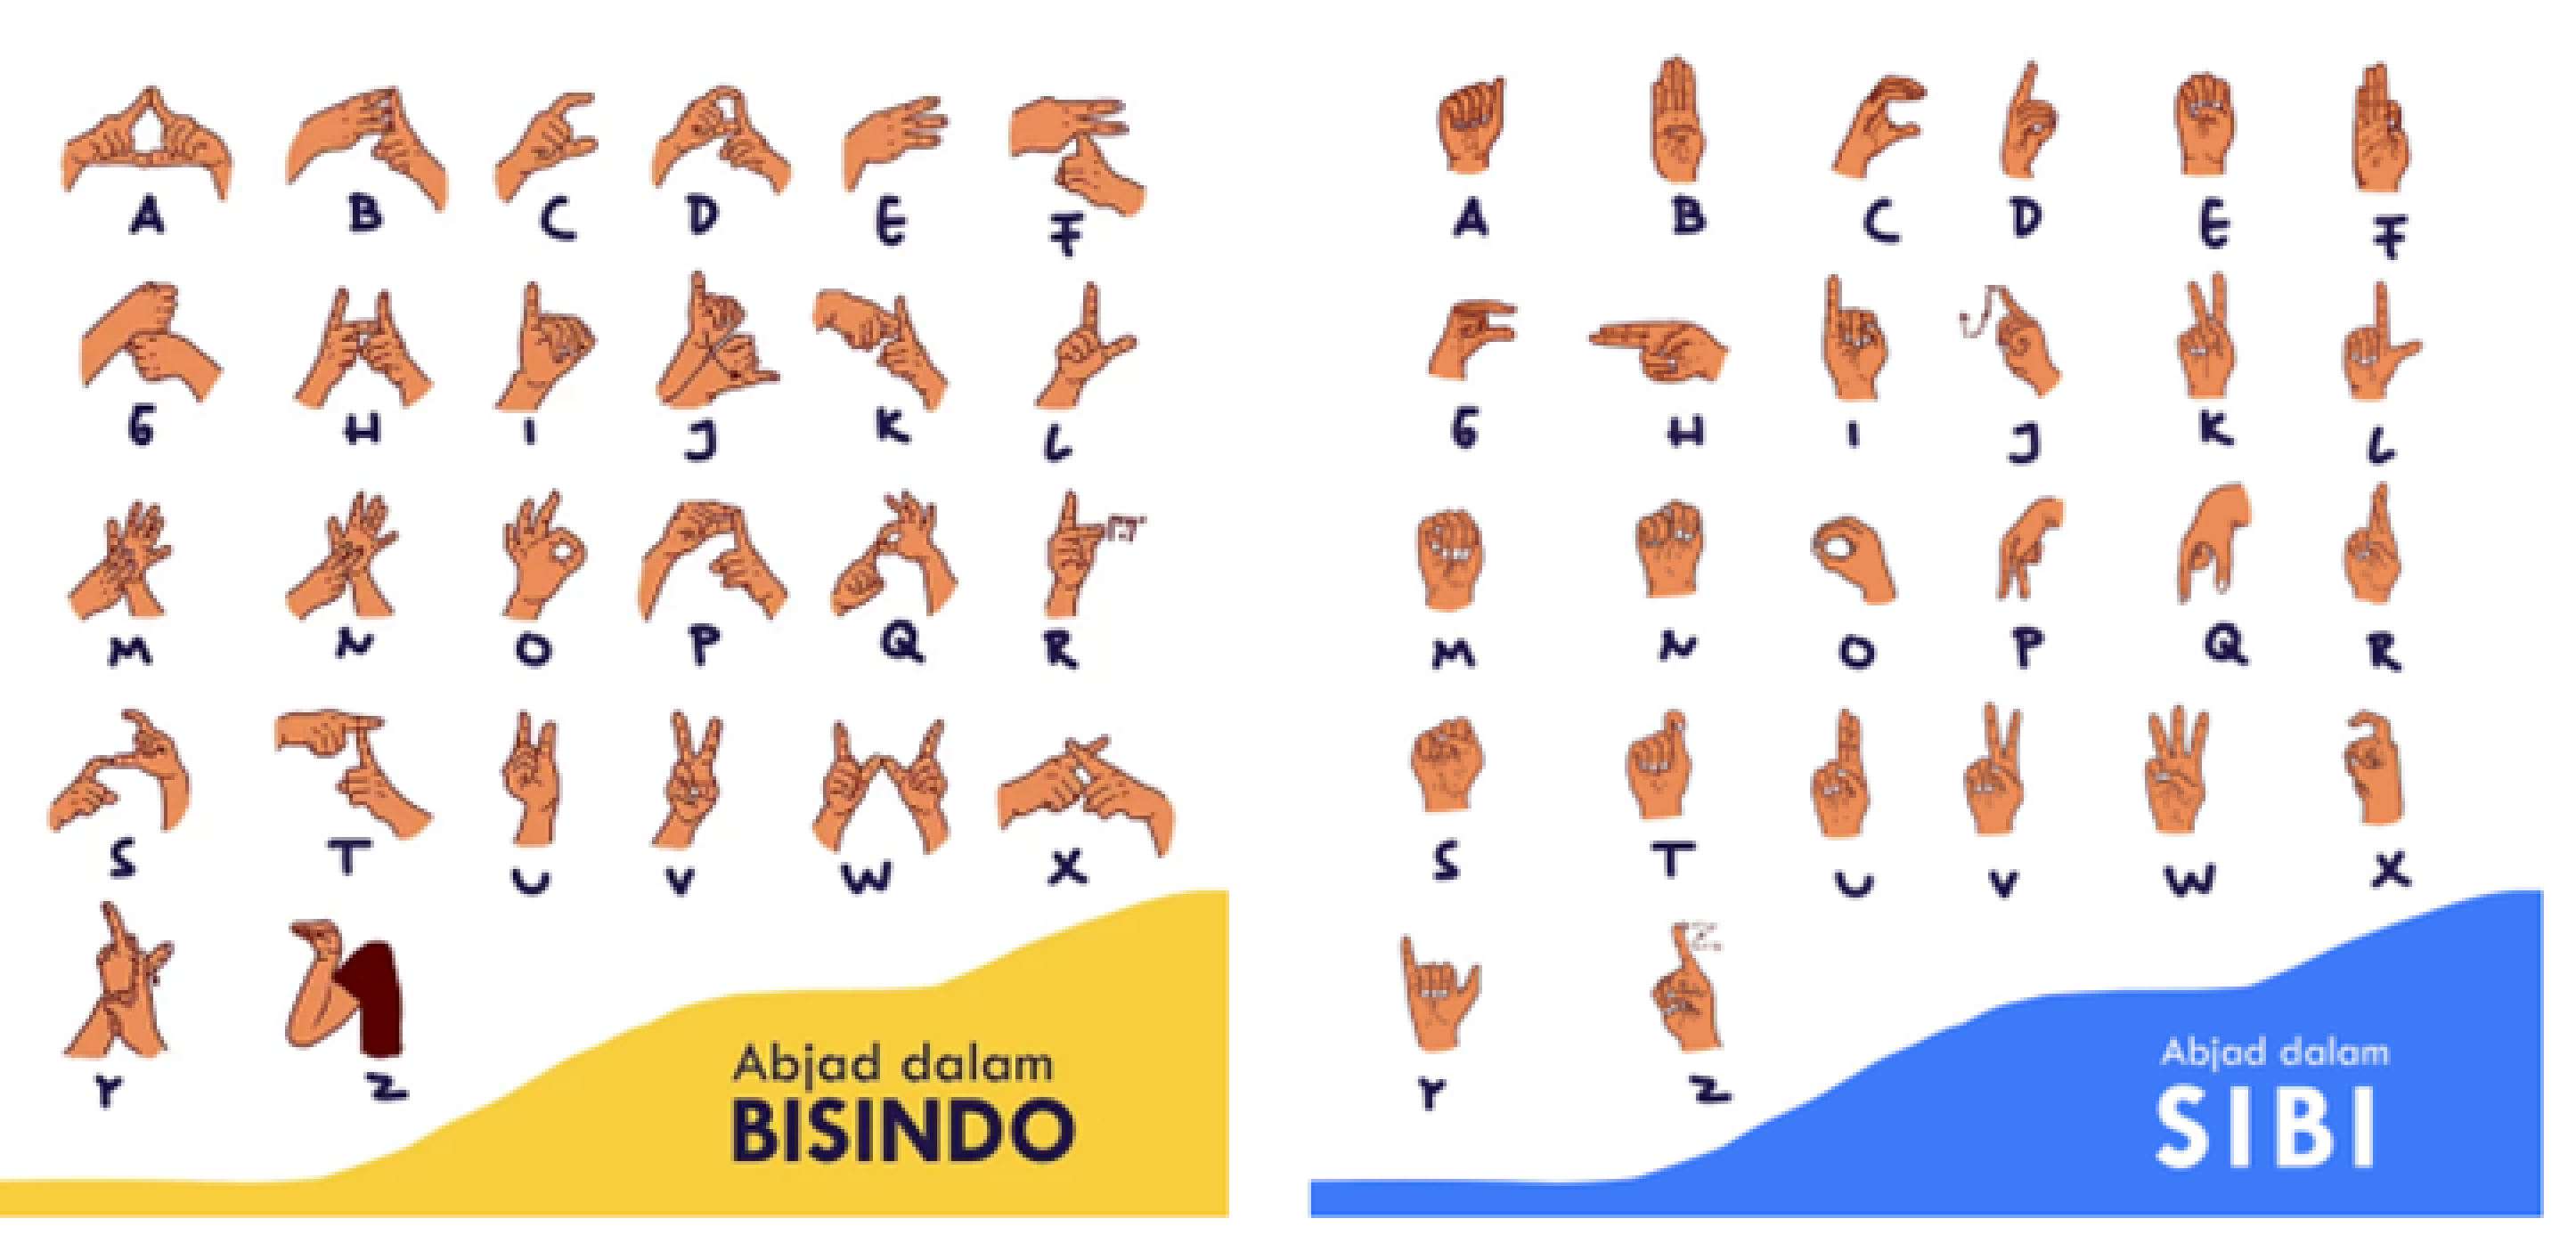
\includegraphics[scale=0.6]{gambar/bab2-isyarat-indonesia.png}
 
%     \caption{Isyarat abjad dalam BISINDO dan SIBI}
%     \label{fig:isyaratindonesia}
% \end{figure}

% Kekurangan pada indra pendengaran yang dialami oleh penyandang tunarungu menyebabkan perkembangan kemampuan berbahasa dan berbicara yang menurun, sehingga banyak dari penyandang tunarungu juga menderita tunawicara. Namun, hal ini bukan menjadi hambatan bagi penderta tunarungu dalam berkomunikasi dengan lingkungan sekitar. Bahasa isyarat adalah bahasa yang dilakukan dengan menggunakan gerakan - gerakan bada yang diiringi dengan ekspresi muka sebagai simbolisasi dari bahasa lisan yang ingin diungkapkan. Tunarungu menggunakan bahasa isyarat sebagai bahasa utama dalam berkomunikasi. Dalam mengungkapkan sesuatu, mereka menggunakan kombinasi antara bentuk tangan, orientasi dan gerak tangan, lengan tubuh, serta ekspresi wajah \parencite{mursita2015}.

% Di Indonesia terdapat 2 bahasa isyarat yang berkembang, yaitu Sistem Bahasa Isyarat Indonesia (SIBI) dan Bahasa Isyarat Indonesia (BISINDO). Berdasarkan gambar \ref{fig:isyaratindonesia}, dapat dilihat bahwa SIBI membentuk isyarat dengan menggunakan 1 tangan saja, sedangkan BISINDO membentuk isyarat menggunakan 2 tangan. BISINDO merupakan isyarat alamiah yang diciptakan dan digunakan sendiri oleh penyandang tunarungu dengan pandangan dan persepsi mereka terhadap segala sesuatu di lingkungan sekitar mereka. Beragam objek atau konsep dapat dinyatakan melalui bahasa isyarat yang mencerminkan bentuk, karakteristik, atau visualnya. Namun, ketika suatu konsep terlalu abstrak untuk direpresentasikan, individu yang tunarungu biasanya akan mengkomunikasikannya dengan memanfaatkan abjad jari \parencite{wedayanti2019}. Tunarungu di Indonesia lebih memilih menggunakan BISINDO sebagai bahasa isyarat yang digunakan dalam kehidupan sehari – hari dibandingkan dengan SIBI karena kemudahan dalam pembentukan isyarat yang tidak terikat pada struktur baku bahasa Indonesia dengan disertai ekspresi wajah dalam pengungkapannya \parencite{handhika2018}. BISINDO sendiri berasal dari bahasa awal atau bahasa ibu tunarungu, dimana penggunaan BISINDO sendiri menyesuaikan dengan pemahaman bahasa tunarungu dari berbagai latar belakang tunarungu dengan tanpa menekankan pada struktur imbuhan bahasa Indonesia \parencite{mursita2015}

% \subsection{MediaPipe}
% MediaPipe merupakan suatu kerangka kerja (\emph{framework}) yang digunakan untuk membantun suatu pipline dalam melakukan inferensi pada data sensorik. MediaPipe memungkinkan untuk membangun suatu pipline yang terdiri dari komponen modular seperti inferensi model, algoritma pemrosesan media, dan transformasi data. Data sensorik seperti audio dan video dapat dimasukkan ke dalam grafik dan menghasilkan \emph{output} berupa deskripsi seperti penentuan objek dan penanda wajah. Kerangka ini mempermudah dalam pembuatan \emph{prototype} cepat dari pipeline persepsi dengan model inferensi dan komponen yang dapat digunakan Kembali. MediaPipe dapat mengabstraksikan dan menghubungkan model – model persepsi individu ke dalam alur yang dapat dipertahankan, dimana hal ini dapat memudahkan dalam penggunaan ulang komponen dalam berbagai aplikasi. Konsep dasar dari MediaPipe terdiri atas tiga bagian utama, yaitu kerangka kerja inferensi data sensorik, seperangkat alat evaluasi kinerja, dan kumpulan komponen inferensi dan pemrosesan yang dapat digunakan kembali. Pipa atau \emph{pipeline} dalam MediaPipe dapat diartikan sebagai grafik komponen yang diarahkan, dimana setiap komponen adalah suatu kalkulator yang spesifik. MediaPipe telah digunakan untuk berbagai aplikasi, termasuk deteksi objek, dan diancang untuk memudahkan dalam pengembangan model machine learning ataupun \emph{ deep learning}, seperti pada deteksi objek dan estimasi pose, terkhususnya pendeteksian gerakan bahasa isyarat \parencite{lugaresi2019:}.

% \subsubsection{Mediapipe Pose}
% Estimasi pose atau pose estimation merupakan suatu aspek yang memiliki peranan penting dalam berbagai teknologi saat ini, seperti mengukur latihan fisik, pengenalan bahasa isyarat, pendeteksian gerakan yoga, menari, dan kebugaran. MediaPipe pose terinspirasi oleh model BlazeFace yang digunakan dalam deteksi wajah Mediapipe, sebagai proksi untuk mendeteksi orang. Model ini dapat dikatakan terinspirasi oleh Virtuvian Leonardo, untuk memperkirakan titik Tengah pinggul seseorang, jari – jari lingkaran yang mengelilingin seluruh orang, dan sudut kemiringan garis yang menghubungkan titik tengah bahu dan pinggul. Model \emph{landmark} dari Mediapipe pose ini memprediksi total 33 lokasi \emph{landmark}, dengan diawali dari bagian hidung hingga diakhiri pada kaki bagian kanan \parencite{googleMediapipe}. 

% \begin{figure}[H]
%     \centering

%     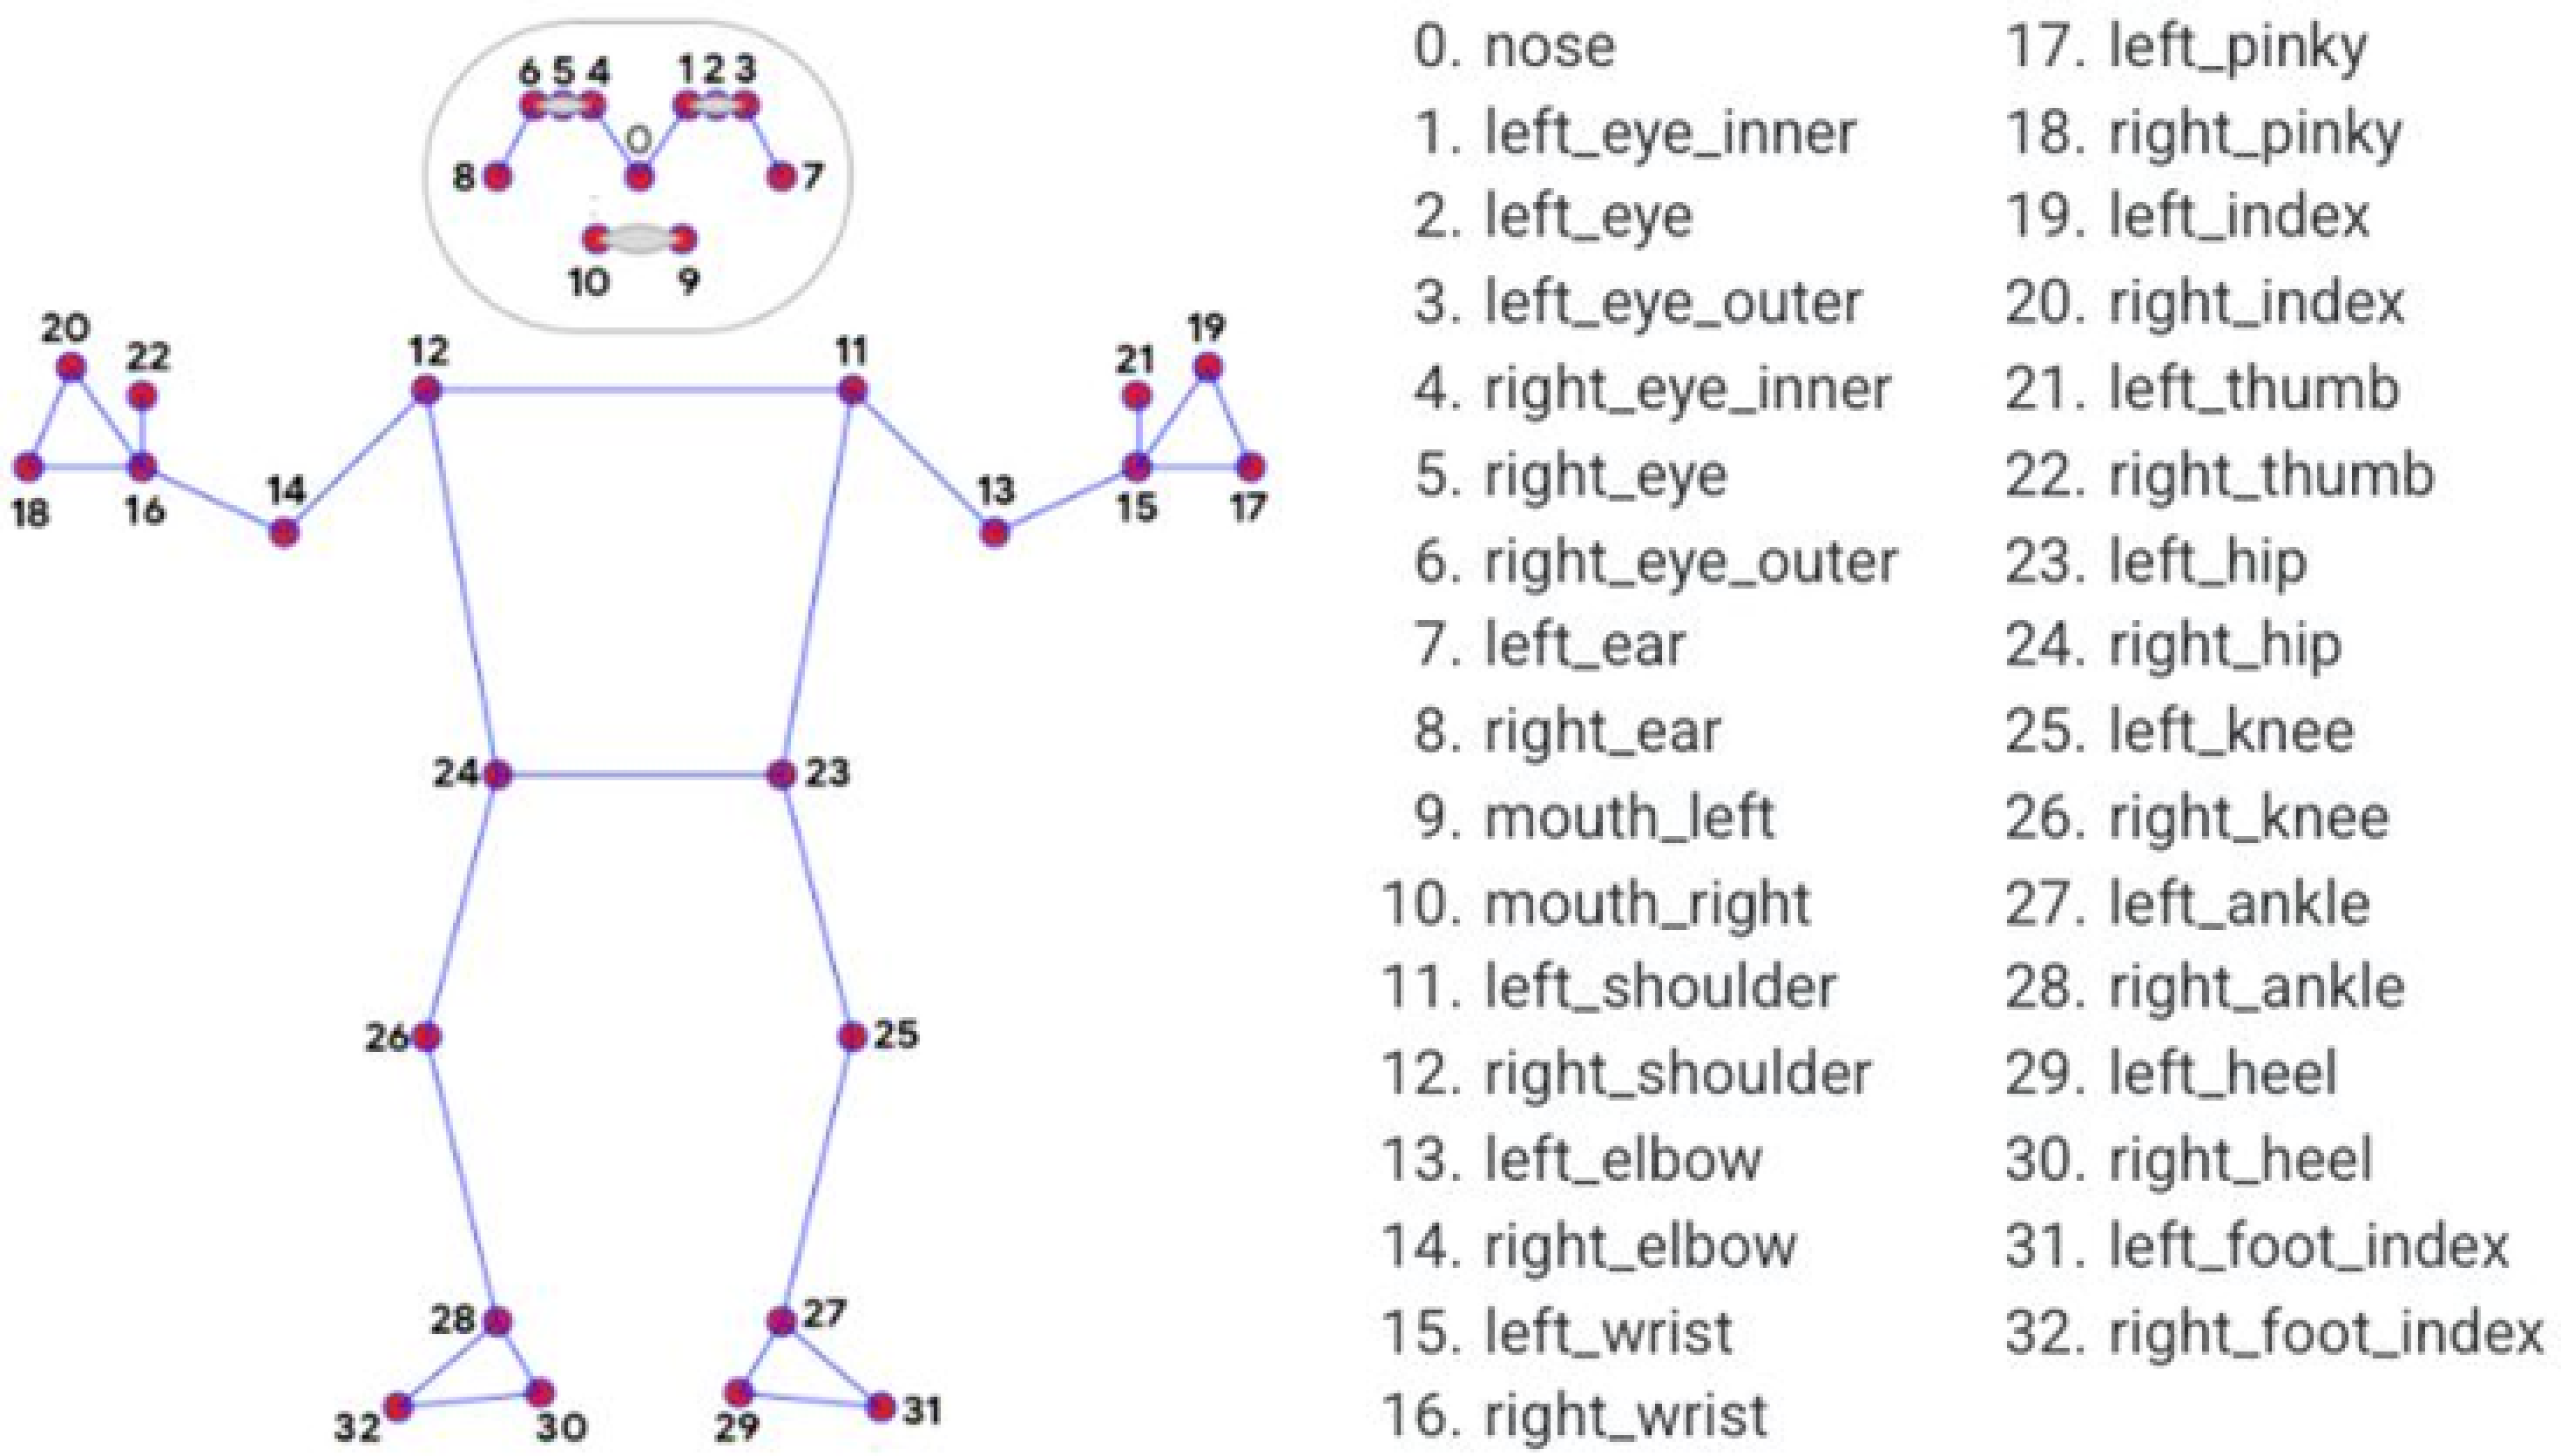
\includegraphics[scale=0.5]{gambar/bab2-mp-pose.png}
 
%     \caption{\textit{Keypoints} \emph{landmark}s pada MediaPipe pose}
%     \label{fig:mediapipepose}
% \end{figure}

% \subsubsection{Mediapipe Hand}
% Kemampuan untuk merasakan bentuk dan gerakan tangan dapat menjadi komponen penting dalam meningkatkan pengalaman pengguna di berbagai platform teknologi, seperti pendeteksian gerakan tangan pada pembentukan bahasa isyarat yang memiliki artinya masing – masing. MediaPipe hand adalah solusi pelacakan tangan dan jari dengan ketelitian tinggi dengan menggunakan \textit{machine learning} untuk menyimpulkan 21 \emph{landmark} 3D tangan dari satu bingkai. Pada setiap ruas jari memiliki \emph{landmark}-nya tersendiri sehingga total \emph{landmark} dari 4 \emph{landmark} dan untuk pangkal telapak tangan terdapat 1 buah \emph{landmark} \parencite{googleMediapipe}.

% \begin{figure}[H]
%     \centering

%     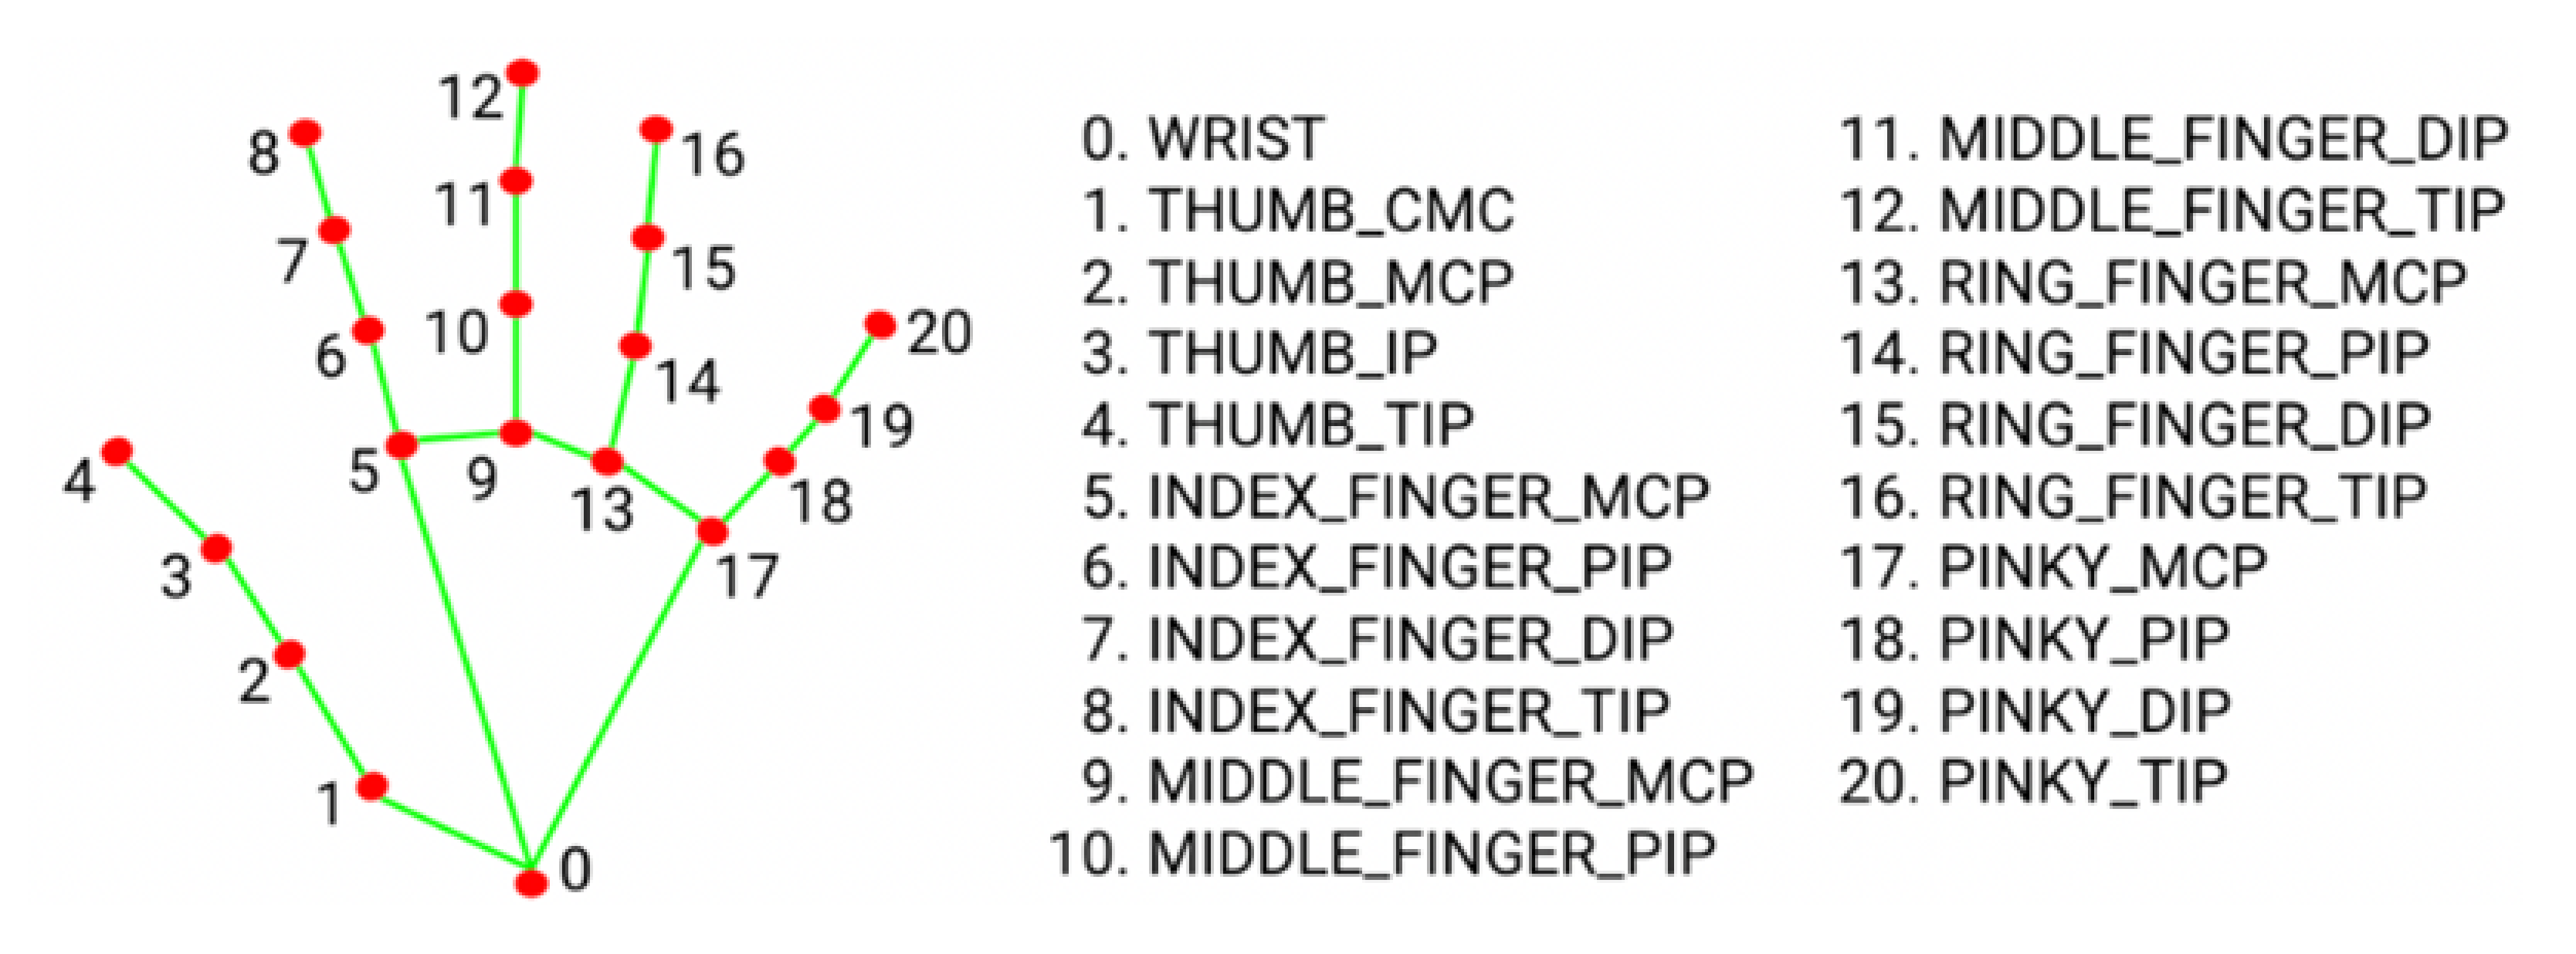
\includegraphics[scale=0.5]{gambar/bab2-mp-hand.png}
 
%     \caption{\textit{Keypoints} \emph{landmark}s pada MediaPipe Hand}
%     \label{fig:mediapipehand}
% \end{figure}

% \subsection{\textit{Long Short-Term Memory} (LSTM)}

% \begin{figure}[H]
%     \centering

%     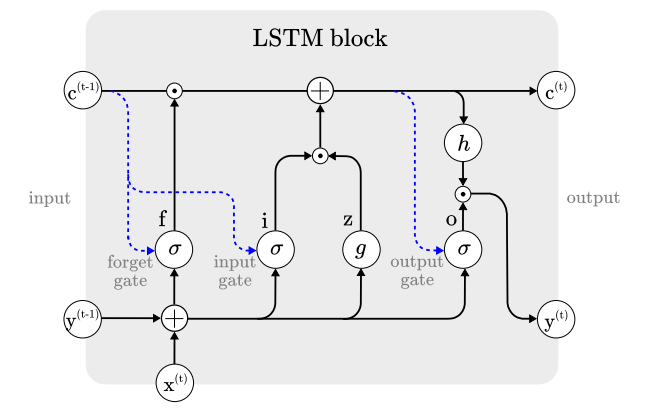
\includegraphics[scale=1.2]{gambar/bab2-lstm-model.png}
 
%     \caption{Cara kerja arsitektur LSTM}
%     \label{fig:longshortterm}
% \end{figure}

% \textit{Long Short-Term Memory} (LSTM) merupakan bentuk khusus dari neural network RNN atau \textit{Recurrent Neural Network} yang memiliki kemampuan \textit{feedback connection}. Kemampuan ini memungkinkan LSTM untuk dapat mengingat informasi untuk waktu yang lama sehingga dapat digunakan untuk menyelesaikan permasalahan yang memiliki sifat sekuensial atau berurutan. Keunggulan LSTM jika dibandingkan dengan RNN adalah LSTM memiliki kemampuan untuk mengingat informasi yang lebih baik dan efektif sehingga meminimalisir terjadinya kehilangan informasi yang umum terjadi pada pemrosesan informasi lama yang panjang pada penggunaan RNN \parencite{xia2020}. Oleh karena itu, LSTM cocok untuk dimanfaatkan dalam pengembangan suatu sistem penerjemah isyarat yang mana membutuhkan kemampuan dalam mengingat gerakan bahasa isyarat yang bersifat sekuensial untuk kemudian disimpan dan diterjemahkan ketika terdapat gerakan yang sesuai.

% Pada gambar \ref{fig:modelLSTM}, \textit{Long Short-Term Memory} tersusun atas beberapa layer yang meliputi \textit{block input}, \textit{input gate}, \textit{forget gate}, \textit{cell}, \textit{output gate}, dan \textit{block output}. \textit{Block input} bertindak untuk melakukan pembaharuan terhadap $x^{(t)}$ dengan \textit{Block input} LSTM unit $y^{(t-1)}$ pada iterasi terakhir. Hal ini dapat dirumuskan sebagai berikut:

% \begin{equation}
%   \label{eq:blockinputLSTM}
%   x^{(t)} = g(W_z x^{(t)} + R_z y^{(t-1)} + b_z)
% \end{equation}

% Pada rumus \ref{eq:blockinputLSTM}, $W_z$ dan $R_z$ merupakan \textit{weight} yang diasosiasikan dengan $x^{(t-1)}$ dan $y^{(t-1)}$ secara berurutan. Sedangkan $b_z$ diartikan sebagai \textit{weight bias vector}. Paada \textit{layer} ini, LSTM   Pada input gate, akan dilakukan pembaharuan terhadap \textit{input} saat ini, ($x^{(t)}$), \textit{output} dari unit LSTM ($y^{(t-1)}$), dan nilai dari \textit{cell} ($c^{(t-1)}$) pada iterasi terakhir. Hal ini  dapat dirumuskan sebagai:

% \begin{equation}
%     \label{eq:inputgateLSTM}
%     i^{(t)} = \sigma(W_i x^{(t)} + R_i y^{(t-1)}+ p_i \odot c^{(t-1)} + b_i)
% \end{equation}

% Pada rumus \ref{eq:inputgateLSTM}, $\odot$ melambangkan perkalian titik antara 2 buah vector. $W_i$, $WR_i$, dan $p_i$ adalah weight yang dimiliki oleh $x^{(t)}$, $y^{(t-1)}$, dan $c^{(t-1)}$. Sementara $b_i$ merepresentasikan bias vector yang diasosasikan oleh unit ini. Forget gate bertindak untuk menentukan informasi yang harus dihapus dari \textit{cell state} ($c^{(t-1)}$) sebelumnya. Oleh karena itu, nilai fungsi aktivasi dari \textit{forget gates} pada \textit{time step} t dihitung berdasarkan input saat ini ($x^{(t)}$), \textit{ouput} ($y^{(t - 1)}$), \textit{state memory cell} ($y^{(t - 1)}$) pada \textit{time step} sebelumnya ($t - 1$), koneksi \textit{peephole}, dan \textit{bias} dari \textit{forget gate} itu sendiri (${b_f}$). \textit{Forget gate} dapat dirumuskan sebagai:

% \begin{equation}
%     \label{eq:forgetgateLSTM}
%     f^{(t)} = \sigma(W_f x^{(t)} + R_f y^{(t-1)}+ p_f \odot c^{(t-1)} + b_f)
% \end{equation}

% Pada rumus \ref{eq:forgetgateLSTM}, $W_f$, $R_f$, dan $p_f$ adalah \textit{weight} yang diasosiasikan dengan $x^{(t)}$, $y^{(t-1)}$, dan $c^{(t-1)}$. Sementara $b_i$ merepresentasikan bias vector yang diasosasikan oleh unit ini. \textit{Cell} merupakan bagian yang melakukan komputasi untuk nilai dari \textit{cell} itu sendiri yang merupakan gabungan dari nilai - nilai pada input $z^{(t)}$, input gate $i^{(t)}$, dan \textit{forget gate} $f^{(t)}$ dengan nilai pada \textit{cell} sebelumnya. Hal ini dapat dirumuskan sebagai:

% \begin{equation}
%     \label{eq:cellLSTM}
%     c^{(t)} =  z^{(t)} \odot  i^{(t)} + z^{(t-1)} \odot  f^{(t)}
% \end{equation}

% Pada \textit{output gate}, akan dilakukan perhitungan untuk \textit{input} saat ini $x^{(t)}$, \textit{output} dari LSTM unit $y^{(t-1)}$, dan nilai cell $c^{(t-1)}$ pada iterasi terakhir. Hal ini dapat dirumuskan sebagai:

% \begin{equation}
%     \label{eq:outputgateLSTM}
%     o^{(t)} = \sigma(W_o x^{(t)} + R_o y^{(t-1)}+ p_o \odot c^{(t)} + b_o)
% \end{equation}

% Pada rumus \ref{eq:outputgateLSTM}, $W_f$, $R_f$, dan $p_f$ adalah\textit{weight} yang diasosiasikan dengan $x^{(t)}$, $y^{(t-1)}$, dan $c^{(t-1)}$. Sementara $b_i$ merepresentasikan \textit{bias vector} yang diasosasikan oleh unit ini. Pada \textit{block otuput}, akan dihitung nilai \textit{cell} saat ini $(c^{(t)})$ dengan nilai output gate saat ini. Hal ini dapat dirumuskan sebagai berikut:

% \begin{equation}
%     \label{eq:blockoutputLSTM}
%     c^{(t)} =  g(c^{(t)}) \odot o^{(t)}
% \end{equation}

% Pada persamaan - persamaan diatas, $\sigma$, $g$, $h$ melambangkan fungsi aktivasi non-linear antar titik. Fungsi logistik \textit{sigmoid} $(\sigma(x) = \frac{1}{1 + e^{-x}})$ digunakan sebagai fungsi aktivasi pada \textit{gate}. Sedangkan fungsi aktivasi \textit{hyperbolic} tangent $g(x) = h(x) = tanh(x)$ digunakan seabagai aktivasi fungsi pada \textit{block input} dan \textit{output} \parencite{van2020}.

% \subsection{Intel \emph{Next Unit Computing} (NUC)}

% \begin{figure}[H]
%     \centering

%     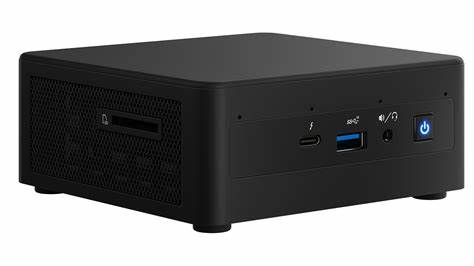
\includegraphics[scale=0.6]{gambar/bab2-nuc_11_performace_kit.jpeg}
 
%     \caption{Intel NUC 11 \emph{Performance Kit}}
%     \label{fig:jetsonnano}
% \end{figure}

% Intel \emph{Next Unit Computing} (NUC) merupakan komputer \emph{barebone} dengan ukuran kecil yang dirancang oleh Intel. Intel NUC merupakan perangkat yang berfokus dalam menyediakan komputasi kuat dalam ukuran yang praktis dan dapat melayani berbagai kebutuhan pengguna, mulai dari bermain \emph{game}, bisnis, hingga menjalankan aplikasi kompleks. Intel NUC secara resmi memperkenalkan perangkat ini pada tahun 2012 dan dipasarkan secara umum pada awal tahun 2013 \parencite{IntelNUC2020}. Adapun seri pertama dari Intel NUC memiliki CPU Sandy Bridger berbasis Celeron. Intel NUC telah berkembang hingga generasi ke-12 bernama Dragon Canyon yang dilengkapi dengan CPU Intel generasi ke-12 dan PCI Express Gen 5 \parencite{Halfacree2013}.

% Intel NUC 11 merupakan perangkat Intel yang dirilis pada 13 Januari 2021 dengan kode nama Phantom Canyon. Salah satu model yang cukup banyak digunakan adalah Intel NUC 11 Performance Kit model NUC11PAHi7. Inti dari perangkat ini dilengkapi dengan prossesor Intel Core i7-1165G7. Prossesor ini memiliki quad-core yang memiliki kecepatan dasar 2.8 GHz dan dapat meningkat hingga 4.7 GHz.  Prossesor ini didukung oleh kartu grafis Iris XE yang menawarkan peningkatan kinerja grafis yang substansial dibandingkan dengan generasi sebelumnya. Hal ini memudahkan perangkat dalam menjalankan tugas mulai dari pengeditan video hingga bermain \emph{game}. Dari segi memori, Intel NUC 11 Performance Kit model NUC11PAHi7 mendukung hingga 64GB DDR4-3200 SODIMM dual-channel, menyediakan ruang yang luas untuk multitasking intensif. Untuk penyimpanan, perangkat ini menawarkan slot M.2 yang fleksibel yang mendukung SSD NVMe terbaru dengan memastikan kecepatan akses dan penyimpanan data yang cepat. Hal ini kritikal untuk aplikasi yang melibatkan set data besar atau pemrosesan \emph{realtime}. Konektivitas adalah salah satu kekuatan utama model ini, menampilkan berbagai pilihan termasuk Thunderbolt 4, HDMI 2.0b, dan beberapa port USB 3.1. Ini memungkinkan koneksi banyak periferal dan tampilan secara bersamaan, meningkatkan produktivitas dan fleksibilitas dalam skenario penggunaan. Selain itu, dengan Intel Wi-Fi 6 dan Bluetooth 5.1, Intel NUC 11 pada model ini menawarkan konektivitas nirkabel terdepan untuk integrasi yang mulus ke dalam lingkungan jaringan apa pun. Dimensi yang ringkas untuk model ini NUC11PAHi70Z, yang hanya berukuran 117 x 112 x 51 mm dapat menjadikannya pilihan ideal untuk lingkungan di mana ruang terbatas \parencite{ASUS2024}. Kombinasi komputasi berkinerja tinggi, kemampuan grafis yang kuat, dan opsi konektivitas yang luas, semua dalam bentuk yang kecil, menonjolkan NUC11PAHi70Z sebagai pilihan teratas bagi pengguna yang membutuhkan solusi komputasi yang kuat, serbaguna, dan efisien ruang.

% % \subsection{Jetson Nano}
% % \begin{figure}[H]
% %     \centering

% %     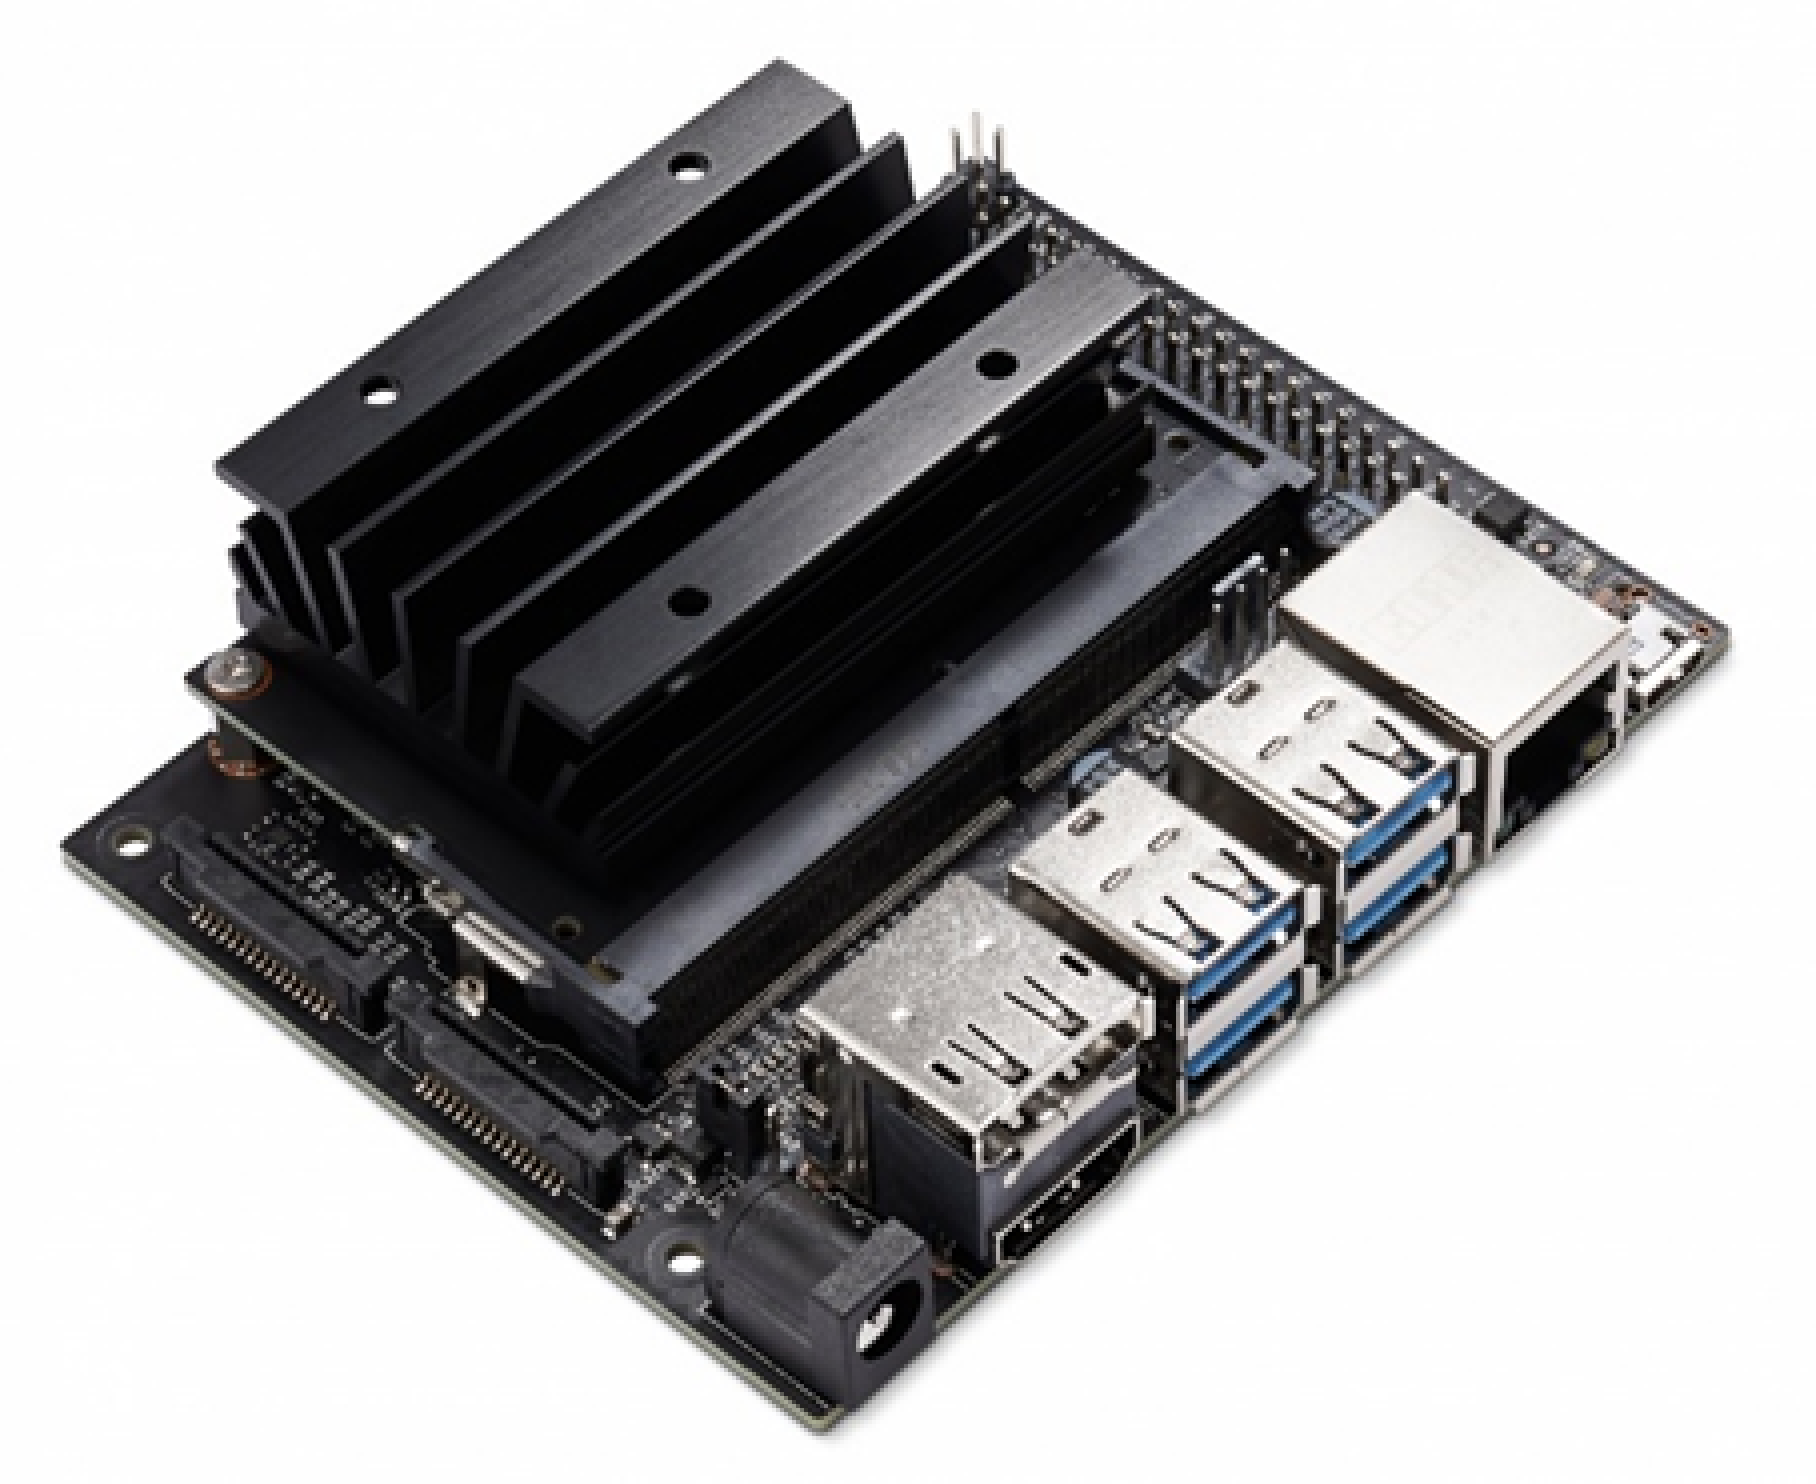
\includegraphics[scale=0.6]{gambar/bab2-jetson-nano.png}
 
% %     \caption{Jetson Nano Developer Kit}
% %     \label{fig:jetsonnano}
% % \end{figure}

% % Jetson Nano adalah perangkat komputasi keluaran NVIDIA yang didedikasikan dalam pengembangan \textit{machine lerarning} dan komputasi edge. Jetson Nano memiliki kemampuan untuk dapat menjalankan beberapa neural networks secara paralel. Kemampuan ini memungkinkan Jetson Nano untuk digunakan dalam \textit{image clasiification}, \textit{object detection}, \textit{segmentation}, dan \textit{speech processing} \parencite{nvidiaJetsonNano}. Perangkat ini dapat menjadi solusi dalam menjalankan model \textit{machine learning} atau \textit{deep learning} pada perangkat portable dan hemat energi. 

% % Perangkat ini dilengkapi dengan 128 NVIDIA CUDA cores. Ditenagai oleh prosesor Quad-core ARM Cortex-A57 MPCore, platform ini menyediakan fungsionalitas komputasi yang solid dengan memori 4 GB 64-bit LPDDR4 yang beroperasi pada 1600MHz, memberikan bandwidth 25.6 GB/s. Untuk penyimpanan, Jetson Nano dilengkapi dengan 16 GB eMMC 5.1, yang memberikan ruang yang cukup untuk aplikasi dan data pengguna. Dalam konteks pengkodean video, perangkat ini dapat mengkodekan video dengan kecepatan 250MP/sec, mendukung format seperti 1x 4K pada 30fps (HEVC), 2x 1080p pada 60fps (HEVC), dan sebagainya. Sementara itu, untuk decode video, perangkat ini menawarkan kemampuan hingga 500MP/sec, dengan dukungan untuk format seperti 1x 4K pada 60fps (HEVC) dan 2x 4K pada 30fps (HEVC). Jetson Nano juga dilengkapi dengan 12 jalur kamera (3x4 atau 4x2) MIPI CSI-2 D-PHY 1.1, yang mendukung kecepatan hingga 1.5 Gb/s per pasangan, memberikan fleksibilitas dalam pengembangan aplikasi berbasis kamera. Dalam hal konektivitas, perangkat ini menawarkan Gigabit Ethernet dan M.2 Key E, serta kemampuan tampilan melalui HDMI 2.0 dan eDP 1.4. Jetson Nano juga dilengkapi dengan 4x USB 3.0 dan USB 2.0 Micro-B, serta berbagai opsi konektivitas lainnya seperti GPIO, I2C, I2S, SPI, dan UART, semuanya dalam form factor mekanis 69.6 mm x 45 mm dengan konektor tepi 260-pin \parencite{nvidiaJetsonNano}.

% \subsection{Performa Klasifikasi}

% \begin{figure}[H]
%     \centering

%     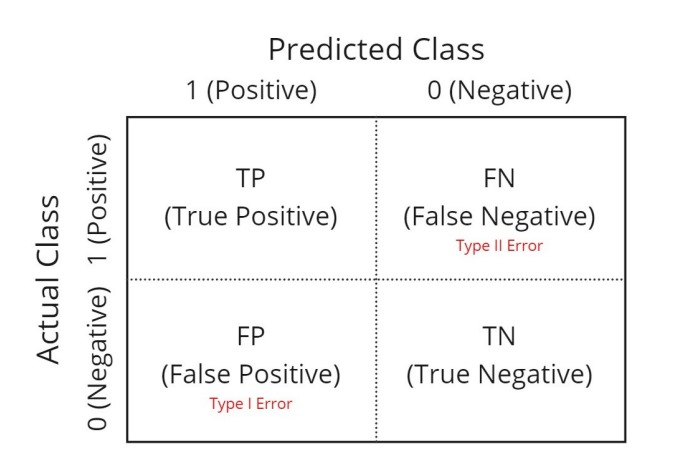
\includegraphics[scale=0.8]{gambar/bab2-confusion-matrix.png}
 
%     \caption{\textit{Confusion matrix}}
%     \label{fig:confusionMatrix}
% \end{figure}

% Dalam melakukan klasifikasi dengan model, diperlukan adanya suatu tolak ukur berdasarkan serangkaian dataset pengujian yang diberikan. Salah satu metode yang dapat digunakan adalah dengan menggunakan \textit{confusion matrix}. \textit{Confusion matrix} merupakan sebuah konsep yang umum digunakan dalam menentukan performa klasifikasi model dengan memberikan informasi mengenai data aktual dan data prediksi model klasifikasi. Berdasarkan \ref{fig:confusionMatrix} \textit{confusion matrix} memiliki bentuk matrix 2 dimensi, dimana satu dimensi memiliki index yang berisikan data aktual dari \textit{class} obyek klasifikasi dan satu dimensi lainnya memiliki index yang berisikan data klasifikasi yang dihasilkan oleh model \parencite{deng2016}. 

% Pada \textit{confusion matrix}, terdapat empat aspek yang digunakan untuk merepresentasikan perbandingan dari kelas aktual dan kelas prediksi. Keempat aspek tersebut meliputi \textit{true positive}, \textit{true negative}, \textit{false positive}, \textit{true negative}. \textit{True positive} (TP) merupakan kondisi dimana data aktual bernilai 1 (positif) diprediksi sebagai data yang bernilai 1 (positif). Sedangkan \textit{true negative} (TN) merupakan kondisi dimana data aktual bernilai 0 (negatif) diprediksi sebagai data yang bernilai 0 (negatif). \textit{False positive} (FP) merupakan kondisi dimana data aktual bernilai 0 (negatif) diprediksi sebagai data yang bernilai 1 (positif). Sedangkan \textit{false negative} (TN) merupakan kondisi dimana data aktual bernilai 1 (positif) diprediksi sebagai data yang bernilai 0 (negatif) \parencite{shajihan2020}. Keempat aspek ini kemudian dapat dihitung nilai \textit{accuracy}, \textit{precision}, \textit{recall}, \textit{F-score} yang dapat membantu dalam memahami performa klasifikasi model dengan lebih detail lagi.

% \subsubsection{\textit{Accuracy}}
% \textit{Accuracy} merupakan metode untuk mengevaluasi kinerja yang menunjukkan tingkat ketep\\atan sebuah model dalam mengklasifikasikan data pengujian yang diberikan secara akurat. \textit{Accuracy} dapat diartikan sebagai perbandingan antara prediksi benar (TP dan TN) terhadap keseluruhan data yang ada. Secara sederhana, \textit{accuracy} menggambarkan seberapa dekat nilai prediksi berada dengan nilai sebenarnya. \textit{Accuracy} dapat dirumuskan dirumuskan pada persamaan \ref{eq:perofrmaAccuracy} \parencite{OvalleMagallanes2020}
   
% \begin{equation}
%     \label{eq:perofrmaAccuracy}
%     Accuracy = \frac{TP + TN}{TP + TN + FP + FN}
% \end{equation}

% \subsubsection{\textit{Precision}}
% \textit{Precision} merupakan metode untuk mengevaluasi kinerja yang mengukur seberapa akurat data yang diminta cocok dengan hasil prediksi yang diberikan oleh model. \textit{Precision} dapat diartikan sebagai perbandingan antara prediksi benar positif (TP) terhadap total hasil yang diprediksi positif (jumlah TP dan FP). \textit{Precision} dapat irumuskan pada persamaan \ref{eq:perofrmaPrecision} \parencite{OvalleMagallanes2020}

% \begin{equation}
%     \label{eq:perofrmaPrecision}
%     Precision = \frac{TP}{TP + FP}
% \end{equation}

% \subsubsection{\textit{Recall}}
% \textit{Recall} merupakan metode untuk menunjukkan kemampuan sebuah model untuk secara akurat mengidentifikasi informasi yang relevan. Recall dapat diartikan sebagai perbandingan antara umlah prediksi benar positif (TP) dengan total jumlah data aktual positif (jumlah TP dan FN). \textit{Recall} dapat dirumuskan pada persamaan \ref{eq:perofrmaRecall} \parencite{OvalleMagallanes2020}

% \begin{equation}
%     \label{eq:perofrmaRecall}
%     Recall = \frac{TP}{TP + FN}
% \end{equation}

% \subsubsection{\textit{F-Score}}

% \textit{F-Score} adalah nilai yang berkisar antara nol hingga satu yang diperoleh dari rata - rata tertimbang (\textit{harmonic mean}) antara nilai precision dan recall. \textit{F-Score} dapat dirumuskan pada persamaan \parencite{Deng2016}

% \begin{equation}
%     \label{eq:perofrmaFScore}
%     F{-}Score = \frac{2 \times {Precision} \times {Recall}}{{Precision} + {Recall}}
% \end{equation}

% \label{subsec:hukumnewton}

% Newton \parencite{newton1687} pernah merumuskan bahwa \lipsum[1]
% Kemudian menjadi persamaan seperti pada persamaan \ref{eq:hukumpertamanewton}.

% Contoh pembuatan persamaan
% \begin{equation}
%   \label{eq:hukumpertamanewton}
%   \sum \mathbf{F} = 0\; \Leftrightarrow\; \frac{\mathrm{d} \mathbf{v} }{\mathrm{d}t} = 0.
% \end{equation}

% \subsection{Anti Gravitasi}
% \label{subsec:antigravitasi}

% Anti gravitasi merupakan \lipsum[1]


% % Contoh input gambar
% \begin{figure}[H]
%   \centering

%   % Ubah dengan nama file gambar dan ukuran yang akan digunakan
%   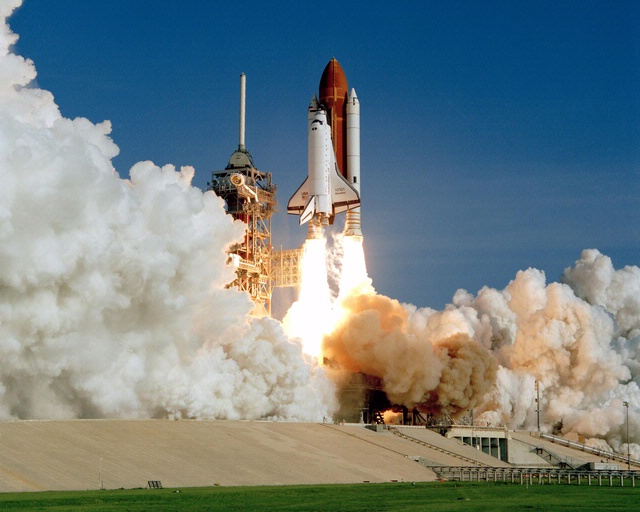
\includegraphics[scale=0.35]{gambar/roketluarangkasa.jpg}

%   % Ubah dengan keterangan gambar yang diinginkan
%   \caption{Peluncuran roket luar angkasa \emph{Discovery} \parencite{roketluarangkasa}.}
%   \label{fig:roketluarangkasa}
% \end{figure}

% Roket luar angkasa merupakan \lipsum[1]

% \emph{Discovery}, Gambar \ref{fig:roketluarangkasa}, merupakan \lipsum[2]
\cleardoublepage

% Bab 3 desain dan implementasi
% \chapter{METODOLOGI}
\label{chap:metodologi}

% Ubah bagian-bagian berikut dengan isi dari desain dan implementasi

Penelitian ini dilaksanakan sesuai \lipsum[1][1-5]
\section{Data dan Peralatan}
Adapun tata pendukung berupa data dan peralatan yang digunakan dalam pelaksanaan penelitian tugas akhir ini adalah sebagai berikut:

\noindent \textbf{Data}\\
Data yang akan digunakan merupakan kumpulan citra berukuran 640px x 480px. Kumpulan citra ini didapat melalui ekstraksi video yang berisi pengucapan bahasa isyarat BISINDO. Kumpulan citra ini dibuat secara mandiri oleh penulis menyesuaikan dengan kebutuhan kosakata isyarat dan kosakata tambahan yang dibutuhkan.

\noindent \textbf{Peralatan}\\
Adapun peralatan yang digunakan dalam penelitian tugas akhir ini adalah sebagai berikut:

\begin{itemize}
  \item Visual Studio Code
  \item Anaconda
  % \item Jetson Nano B01 Developer Kit
  \item Intel Next Unit Computing (NUC) 
  \item Webcam
  \item Speaker
  \item Laptop
\end{itemize}

Tugas akhir ini akan dilaksanakan sesuai dengan desain sistem beserta implementasinya yang akan dibahas pada bab ini. Desain sistem ini merupakan konsep dasar perancangan dan pembuatan program pada tugas akhir ini. Desain sistem ini direpresentasikan dalam bentuk blok diagram yang diselesaikan secara bertahap dan menyeluruh.

\section{Metode yang Digunakan}

% Penelitian tugas akhir ini dilaksankaan sesuai dengan desain sistem yang tertera pada bab ini. Desain sistem yang dibuat merupakan konsep dari perancangan dan implementasi penelitian ini. Blok diagram pada gambar \ref{fig:blockdiagrammethod} merupakan serangkaian alur yang diikuti dalam pelaksanaan dan pengimplementasian tugas akhir ini.

Adapun tugas akhir ini merupakan pengembangan dari teknologi visi komputer yang kemudian diimplementasikan pada Intel \emph{Next Unit Computing} (NUC). Secara umum, pelaksanaan tugas akhir ini didasari oleh blok diagram yang dapat dilihat pada gambar \ref{fig:blockdiagrammethod}.

\begin{figure}[H]
  \centering

  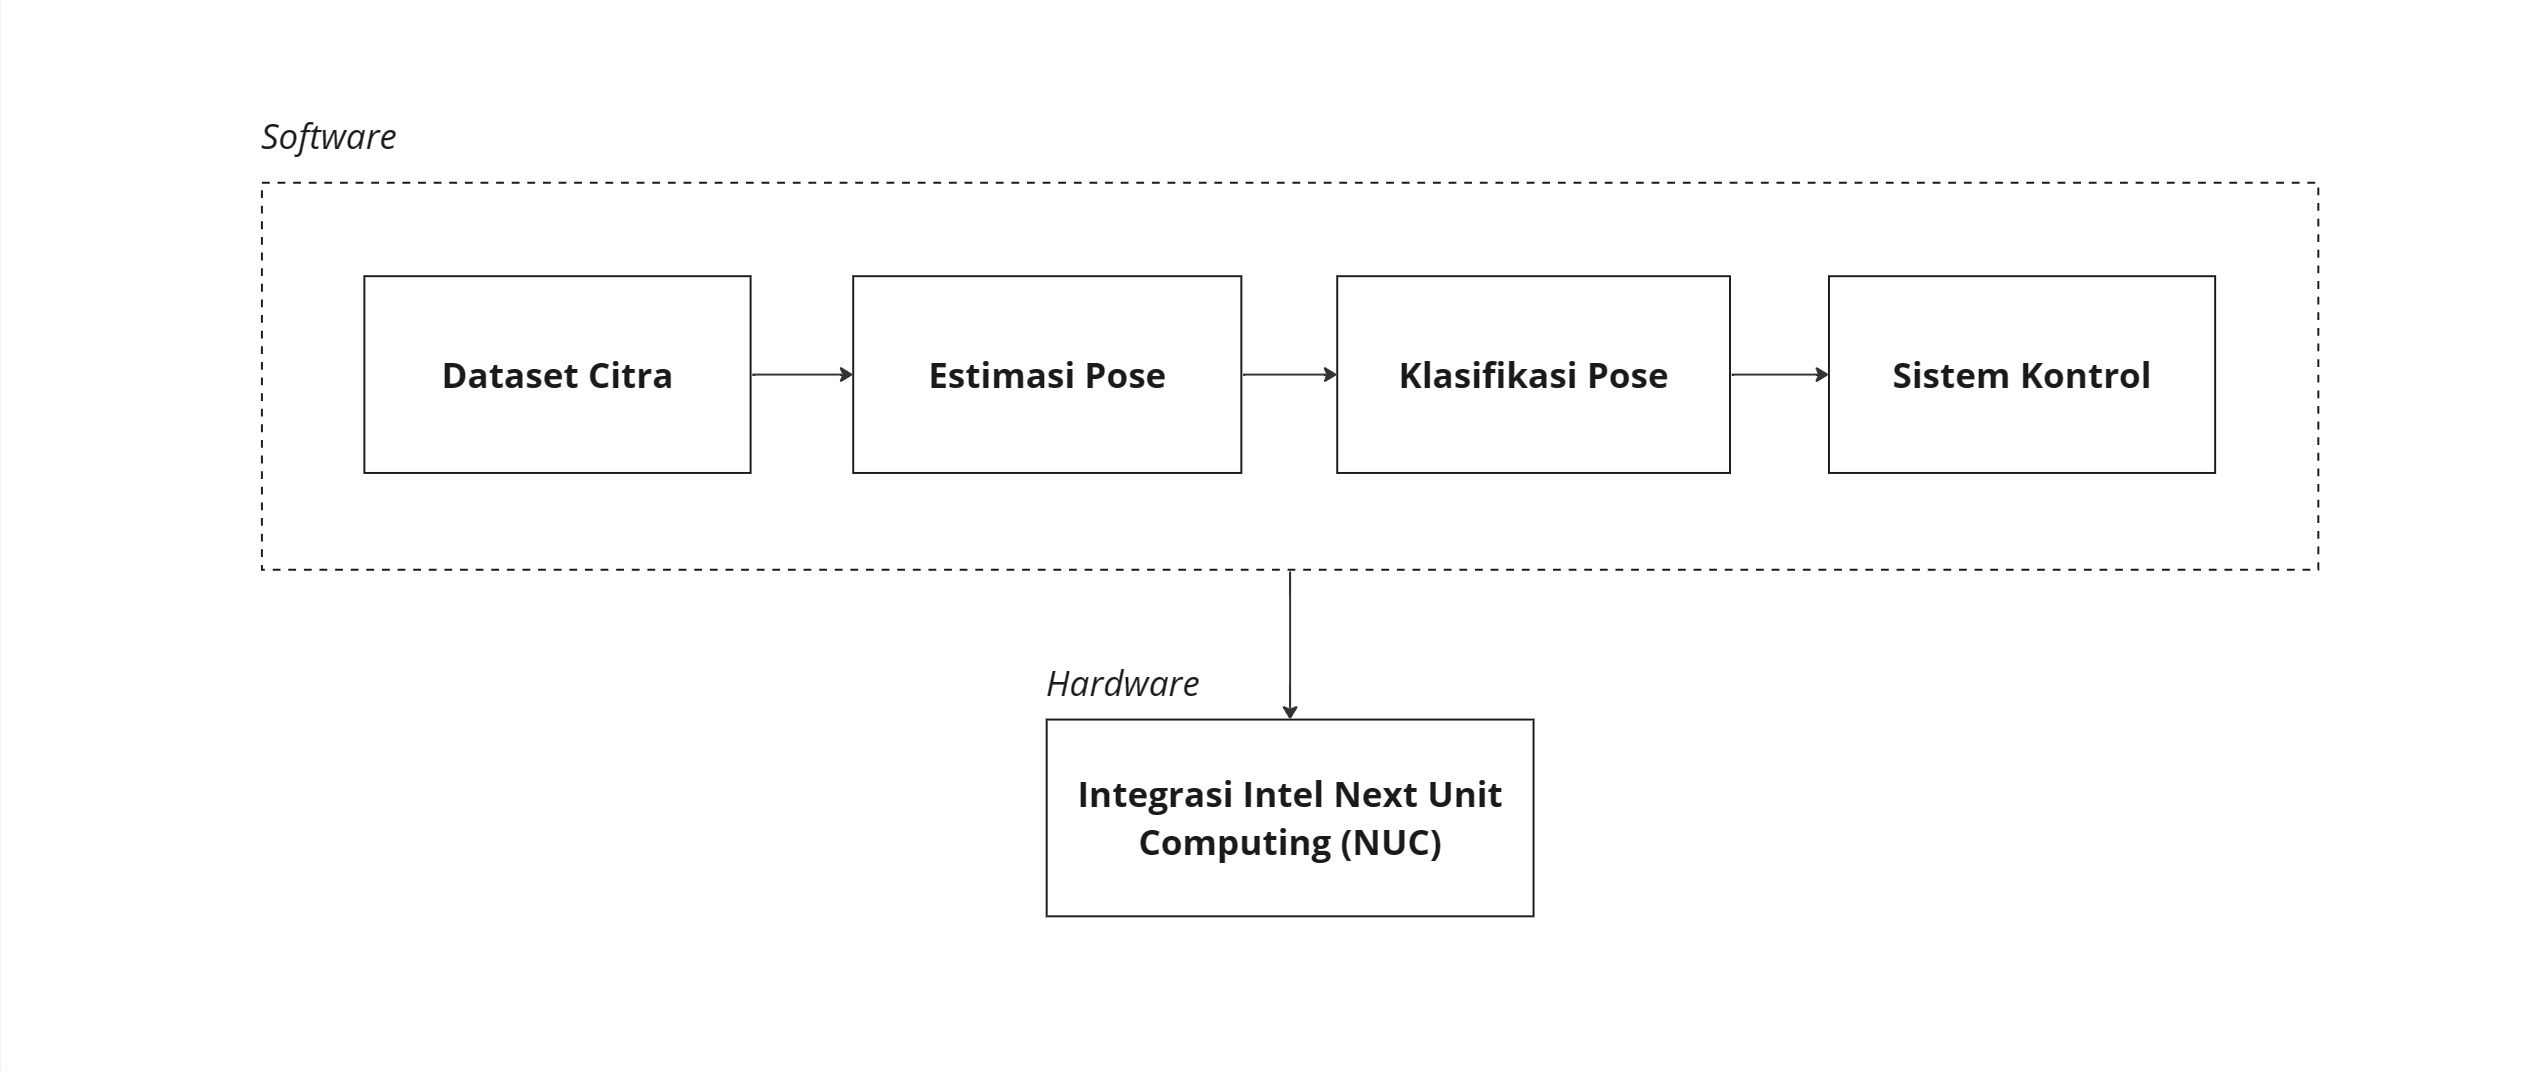
\includegraphics[scale=0.16]{gambar/bab3-block-diagram-nuc.jpg}

  \caption{Blok diagram metodologi}
  \label{fig:blockdiagrammethod}
\end{figure}

\subsection{Dataset Citra}
\label{sec:metodologidataset}

% Dataset yang akan digunakan pada tugas akhir ini merupakan kumpulan citra yang berbentuk sekuensial atau berurutan. Pengambilan dataset dilakukan di dalam ruangan tertutup dengan jarak bervariasi antara 1 - 2 meter dari kamera laptop dengan posisi setengah berdiri (dari pinggang hinga kepala). Data video yang didapatkan kemudian diproses melalui \textit{library} Python OpenCV sehingga dihasilkan citra. Pengambilan citra dilakukan sebesar 30 \textit{frame per second} (FPS) sehingga dalam satu detik terdapat 30 citra. Pembatasan FPS ini diharapkan dapat memberikan hasil yang stabil dan konsisten dalam pengambilan citra. Citra akan disimpan pada laptop secara lokal sehingga dapat diamati nantinya apakah gerakan bahasa isyarat yang dilakukan telah benar atau tidak dan menghasilkan dataset yang baik digunakan dalam pembuatan model klasifikasi. Dapat dilihat pada gambar \ref{fig:datasetMethod} akan dihasilk total 30 citra. Perlu diperhatikan bahwa ukuran dari citra yang akan digunakan pada tugas akhir ini adalah sebesar 640px x 480px

Dataset yang akan digunakan dalam pelaksanaan tugas akhir ini merupakan kumpulan citra dalam bentuk sekuensial atau berurutan. Pengambilan dataset akan dilakukan di dalam ruangan tertutup dengan jarak antara kamera dengan penulis bervariasi antara 1 - 2 meter dari kamera laptop. Posisi penulis terhadap kamera adalah dalam keadaan berdiri. Akan didapatkan data berupa video melalui bantuan \emph{library} OpenCV. Video yang diambil merupakan kumpulan dari total 30 \emph{frame} atau citra sebesar 640 pixel x 480 pixel. Pembatasan ini ditujukan untuk membuat dataset dengan hasil yang stabil dan konsisten dalam semua gerakan isyarat yang dilakukan. Dataset akan disimpan pada laptop secara lokal untuk nantinya diamati apakah gerakan isyarat BISINDO yang dilakukan telah benar dan menunjukkan keunikan dari masing - masing kosakata. Hal ini penting diamati untuk menghasilkan model LSTM dengan performa klasifikasi yang baik. Contoh satu data yang merepresentasikan gerakan isyarat untuk kosakata "nama" dapat dilihat pada gambar \ref{fig:datasetMethod}.

\begin{figure}[H]
  
  \centering

  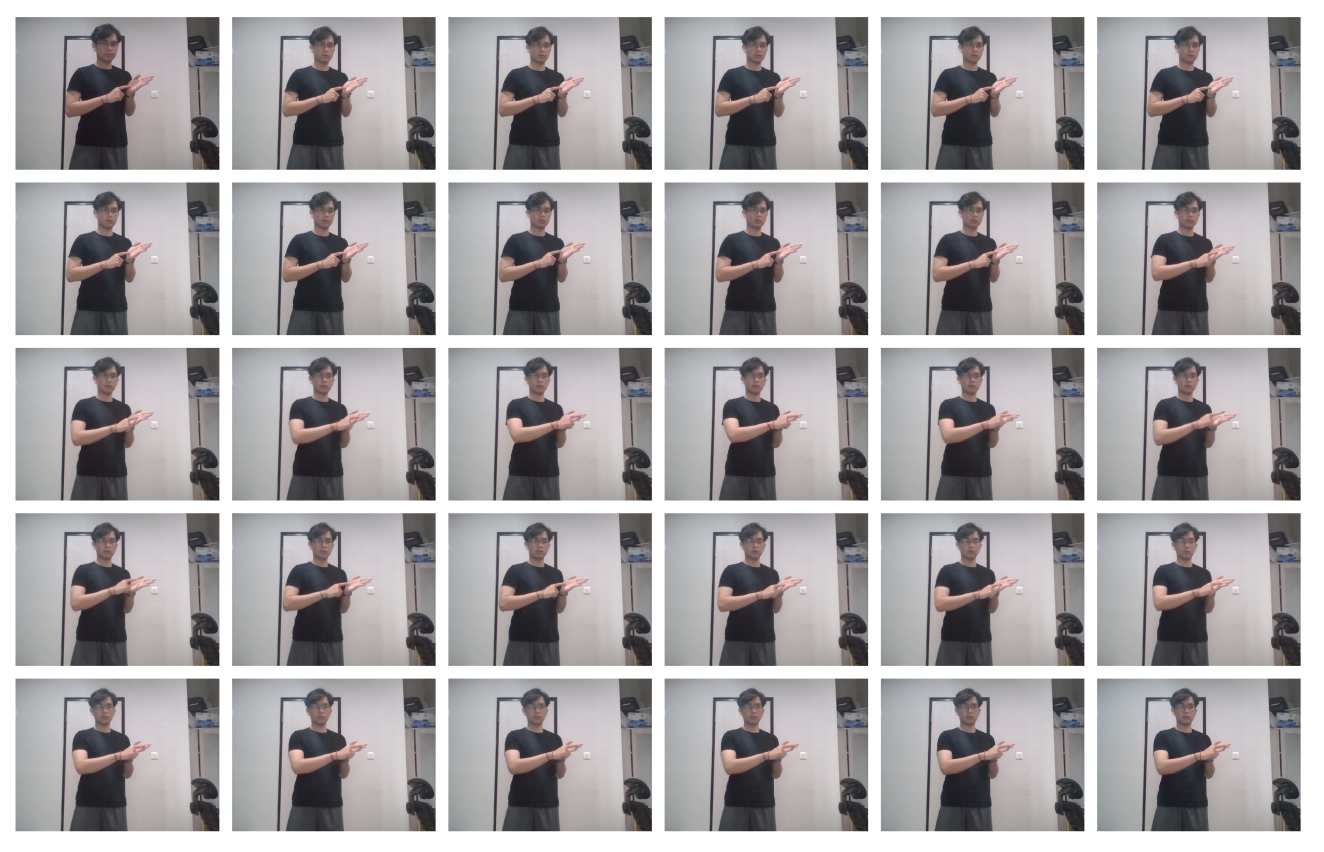
\includegraphics[scale=0.5]{gambar/isyarat-clear-nama.png}

  \caption{Dataset kosakata "nama"}
  \label{fig:datasetMethod}
\end{figure}

Adapun bahasa isyarat yang akan digunakan pada tugas akhir ini meliputi 6 kosakata isyarat BISINDO yang memiliki konteks kalimat yang umum digunakan sehari – hari. Nantinya untuk setiap kosakata tersebut akan disimpan sebanyak 30 jumlah data dengan masing - masing data terkumpul sebanyak 30 \emph{frame}. Kosakata yang akan digunakan adalah sebagai berikut:

\begin{longtable}{|c|c|c|c|}
  \caption{Kosakata BISINDO}
  \label{tb:kosakataBISINDO}                                   \\
  \hline
  \rowcolor[HTML]{C0C0C0}
  \textbf{No} & \textbf{Kelas} & \textbf{Jumlah Data} & \textbf{Jumlah \emph{Frame}}\\
  \hline
  1            & Maaf                       & 30            & 30\\
  2            & Tolong                     & 30            & 30\\
  3            & Saya                       & 30            & 30\\
  4            & Nama                       & 30            & 30\\
  5            & Rumah                       & 30            & 30\\
  6            & Siapa                       & 30            & 30\\
  \hline
\end{longtable}

% Digunakan tambahan 3 buah isyarat tambahan di luar isyarat BISINDO untuk mempermudah kontrol sistem penerjemah. Isyarat tersebut meliputi isyarat mulai (\textit{start}), isyarat \textit{standby}, isyarat hapus kata (\textit{delete}), dan isyarat terjemah (\textit{translate}).  

Dalam mempermudah kontrol sistem penerjemah, digunakan 3 gerakan isyarat tambahan di luar gerakan isyarat BISINDO.  Isyarat tersebut meliputi isyarat \textit{standby}, isyarat hapus kata (\textit{delete}), dan isyarat terjemah menjadi suara (\textit{translate}).  Untuk setiap gerakan isyarat kontrol juga memiliki jumlah data yang sama dengan gerakan isyarat BISINDO, yaitu 30 data dengan 30 \emph{frame} pada setiap datanya.

\begin{longtable}{|c|c|c|c|}
  \caption{Isyarat Kontrol Tambahan}
  \label{tb:isyaratkontrol}                                   \\
  \hline
  \rowcolor[HTML]{C0C0C0}
  \textbf{No} & \textbf{Kelas} & \textbf{Jumlah Data} & \textbf{Jumlah \emph{Frame}}\\
  \hline
  1            & \textit{Standby}                       & 30             & 30 \\
  2            & \textit{Translate}                     & 30             & 30 \\
  3            & \textit{Delete}                        & 30             & 30 \\
  \hline
\end{longtable}
\newpage
\subsection{Estimasi Pose}

\begin{figure}[H]
  \centering

  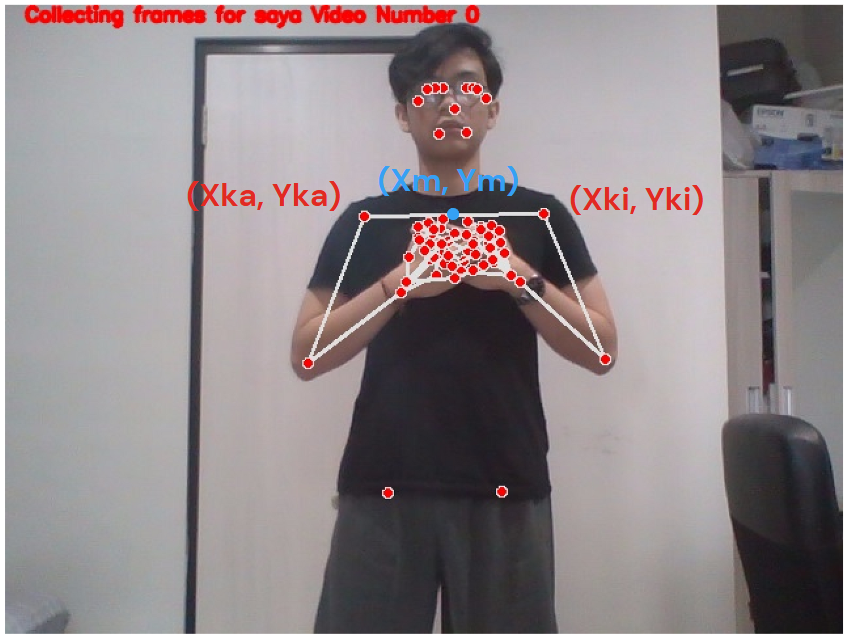
\includegraphics[scale=0.6]{gambar/bab3-estimasi-pose.png}

  \caption{Estimasi pose pada citra}
  \label{fig:poseEstimationMethod}
\end{figure}

Untuk setiap citra pada 30 data yang telah dilakukan estimasi pose dengan bantuan \textit{framework} MediaPipe. \textit{Framework} ini dapat melacak titik – titik bagian tubuh atau \textit{landmark} menggunakan model yang disediakan. Model MediaPipe yang akan digunakan adalah MediaPipe pose dan MediaPipe hand. Dalam pembentukan isyarat BISINDO, bagian tubuh yang bergerak adalah bagian tangan dan lengan. Melalui MediaPipe hand akan dilakukan ekstraksi untuk 21 \textit{landmark} pada bagian tangan, sehingga total \textit{landmark} untuk tangan kanan dan kiri adalah 42 \textit{landmark}. Kemudian melalui MediaPipe pose akan dilakukan ekstraksi pada bagian bahu sampai lengan sehingga \textit{landmark} yang akan digunakan hanya pada posisi 11 hingga 22 sehingga total \textit{landmark} untuk bagian tubuh adalah 12 \textit{landmark}. Untuk setiap \textit{landmark} yang didapatkan akan digunakan koordinat x dan y saja (koordinat z dan \textit{visibility} tidak digunakan). Hal ini berguna demi menghasilkan model akhir yang memiliki kemampuan untuk invarian terhadap skala (jarak kamera tidak mempengaruhi estimasi pose) dan invarian terhadap rotasi (adanya rotasi tidak mempengaruhi koordinat yang digunakan). Hal ini juga dilakukan demi melakukan reduksi dimensi sehingga mengurangi resiko \textit{overfitting} dan dapat mempercepat performa model. Nantinya, untuk setiap citra yang akan diproses pada MediaPipe akan menghasilkan total 42 koordinat dari \textit{landmark} tangan kanan, 42 koordinat dari \textit{landmark} tangan kiri, dan 24 koordinat dari \textit{landmark} pose.Hal ini dapat dilihat pada gambar \ref{fig:poseEstimationMethod}, \textit{landmark} yang akan digunakan hanyalah \textit{landmark} yang saling terhubung (ditandai dengan garis putih). Sedangkan \textit{landmark} yang hanya berbentuk titik saja tidak akan digunakan dan tidak akan diambil data koordinatnya. Data koordinat \textit{landmark} yang berbentuk array multidimensi kemudian akan diproses melalui \textit{library} Numpy dengan menggunakan fungsi concatenate menjadi satu dimensi saja untuk mempermudah pada klasifikasi pose pada tahap \textit{training} data.

\subsubsection{Normalisasi Data}
Keseluruhan data koordinat yang didapatkan melalui estimasi pose menggunakan MediaPipe akan melalui proses normalisasi. Normalisasi data dilakukan demi mengatasi adanya \textit{scale invariant} dan \textit{position invariant}. \textit{Scale invariant} dalam konteks tugas akhir ini adalah kemampuan model dalam mengklasifikasikan data bahasa isyarat yang dilakukan oleh berbagai macam pengguna yang memiliki bentuk tubuh yang berbeda - beda. Selain itu, \textit{scale invariant} juga menyebabkan jarak pengguna dengan kamera tidak mempengaruhi proses klasifikasi model. \textit{Position invariant} dalam konteks tugas akhir ini adalah kemampuan model dalam mengklasifikasikan data bahasa isyarat dalam berbagai posisi pengguna terhadap kamera (dengan catatan bahwa posisi tangan dan bahu dapat terlihat jelas ketika pengguna melakukan gerakan isyarat).

\begin{equation}
  \label{eq:shouderWidthNorm}
  w = \sqrt{(x_{ka} - x_{ki})^2 + (y_{ka} - y_{ki})^2}
\end{equation}

\begin{equation}
  \label{eq:shoulderMidpointNorm}
  x_m = \frac{x_{ka} + x_{ki}}{2} ; \\
   y_m = \frac{y_{ka} + y_{ki}}{2}
\end{equation}

\begin{equation}
  \label{eq:normalization}
  x'_i = \frac{x_i - x_m}{w} ;  \\
   y'_i = \frac{y_i - y_m}{w}
\end{equation}

Dalam melakukan proses normalisasi, terlebih dahulu didapatkan panjang dari bahu dengan menggunakan rumus jarak \textit{Euclidian}. Rumus ini akan menghitung kuadrat selisih antara koordinat x dan y antara \textit{landmark} bahu kanan dan kiri. Hasil dari kedua operasi tersebut kemudian dijumlahkan dan dihitung akar kuadratnya. Perhitungan jarak \textit{Euclidian} dapat dapat dilihat pada rumus \ref{eq:shouderWidthNorm}. Untuk mendapatkan titik tengah dari \textit{landmark} bahu, dilakukan dengan menjumlahkan masing - masing koordinat x dan y dari bahu kanan dan kiri, kemudian dibagi dengan 2. Proses ini dapat dilihat pada rumus \ref{eq:shoulderMidpointNorm}.

Normalisasi data akan dilakukan dengan melakukan pengurangan terhadap setiap koordinat \textit{landmark} dengan koordinat titik tengah dari bahu dan diakhiri dengan pembagian dengan panjang dari bahu yang telah dihitung sebelumnya. Hal ini dapat dilihat pada rumus \ref{eq:normalization}. Perlu diketahui bahwa pada perumusan diatas, $w$ adalah panjang bahu, $x_{ka}$ adalah koordinat x bahu kanan, $y_{ka}$ adalah kooridnat y bahu kanan, $x_{ki}$ adalah koordinat x bahu kiri, $y_{ki}$ adalah kooridnat y bahu kiri, $x'_i$ adalah koordinat x yang telah dinormalisasi, dan $y'_i$ adalah kooridnat y yang telah dinormalisasi.

Nantinya data koordinat yang telah dinormalisasi ini akan disimpan dalam bentuk array dengan bantuan Numpy dan akan digunakan dalam proses \textit{training}. Normalisasi data tidak hanya digunakan dalam proses pembuatan model, tetapi juga nantinya dalam proses klasifikasi bahasa isyarat dengan menggunakan model. Hal ini dilakukan sehingga koordinat - kooridnat yang diproses adalah homogen dan menghindari adanya \textit{noise} atau \textit{error}.

\subsection{Klasifikasi Pose}
\label{sec:metodologipose}

Dalam melakukan klasifikasi terhadap pose atau gerakana isyarat yang dilakukan, digunakan model LSTM dengan bentuk sekuensial sehingga dapat menggabungkan serangkaian \emph{layer} untuk menghasilkan model penerjemah bahasa isyarat yang memiliki performa baik. \emph{Layer} pertama merupakan \emph{layer} \textit{TimeDistributed} yang di dalamnya terdapat \emph{layer} \textit{Dense} dengan jumlah unit sebesar 128, fungsi aktivasi '\textit{tanh}' dan input dengan bentuk (30, 108). Penggunaan \textit{TimeDistributed} memastikan bahwa untuk setiap frame (data input) akan diproses secara independen. Pada \emph{layer} ini diimplementasikan \emph{layer} \textit{Dense} yang konsisten pada setiap frame yang ada. Hal ini berguna untuk memastikan bahwa representasi dari data yang dipelajari menjadi konsisten pada setiap iterasi pembelajaran model. Cara kerja \emph{layer TimeDistributed} secara garis besar dapat dilihat pada gambar \ref{fig:layerTimeDistributed}. Perlu diperhatikan bentuk data (30, 108) berarti akan terdapat 30 jumlah frame, dimana untuk setiap frame akan diekstrak total 108 fitur. 108 fitur tersebut merupakan kumpulan dari data koordinat x dan y untuk setiap \emph{landmark} Mediapipe yang digunakan.\emph{Layer} kedua merupakan LSTM pertama yang memiliki jumlah unit 128, return\_sequences=True, fungsi aktivasi '\textit{tanh}', dan input dalam bentuk (30, 108). Pada \emph{layer} ketiga diikuti dengan \emph{layer} Dropout dengan nilai 0.5 untuk menghindari adanya nilai \emph{weight} yang terlalu tinggi. \emph{Layer} selanjutnya, yaitu \emph{layer} keempat merupakan layer LSTM kedua yang memiliki jumlah unit 128, return\_sequences=False, dan fungsi aktivasi '\textit{tanh}'. Pada \emph{layer} kelimat diikuti dengan \emph{layer} Dropout dengan nilai 0.5 untuk menghindari adanya nilai \emph{weight} yang terlalu tinggi. Dapat dilihat bahwa untuk setiap \emph{layer} LSTM memiliki \emph{layer} Dropout untuk menghindari \emph{overfitting} pada model dengan menonaktifkan \emph{neuron} dengan probabilitas sebesar 50\%. 

\begin{figure}[H]
  \centering

  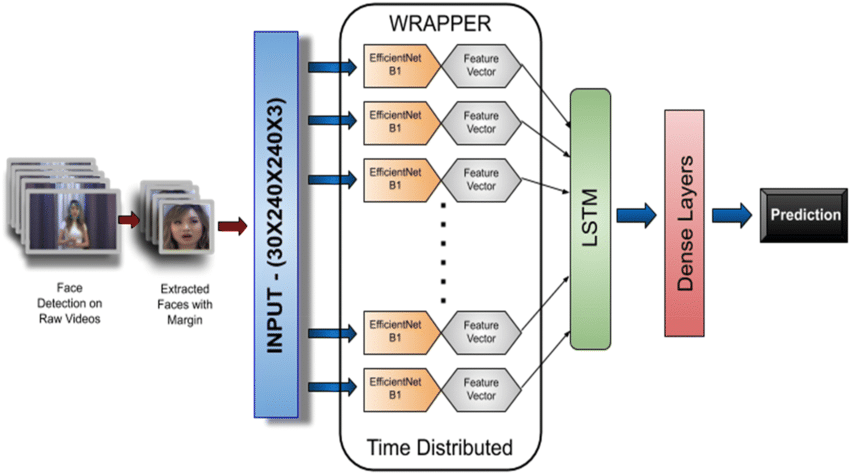
\includegraphics[scale=0.45]{gambar/layer-timedistributed.png}

  \caption{Cara kerja \emph{layer Time Distributed} \parencite{Singh2020}}
  \label{fig:layerTimeDistributed}
\end{figure}

Untuk menyederhanakan kompleksitas dari data output yang diberikan 2 layer LSTM, digunakan \emph{layer} Dense dengan jumlah unit 128 dan fungsi aktivasi 'relu'. Setelah \emph{layer} \textit{Dense}, diberikan \emph{layer} Dropout dengan nilai 0.2 untuk menghindari adanya kelebihan \emph{overfitting} pada model. \emph{Layer} terakhir adalah \emph{layer} \textit{Dense} yang menggunakan fungsi aktivasi '\textit{softmax}'. Jumlah unit di \emph{layer} ini sesuai dengan actions.shape[0], yang berarti jumlah unit sama dengan jumlah aksi atau kategori yang mungkin. Fungsi aktivasi '\textit{softmax}' memastikan bahwa keluaran dari model ini adalah distribusi probabilitas di atas semua kategori yang mungkin, dengan total semua probabilitas sama dengan 1. Model ini kemudian dikompilasi menggunakan \emph{optimizer} Adam, yang dikenal karena performa dan efisiensinya dalam pelatihan jaringan saraf, dan menggunakan \textit{categorical crossentropy} sebagai fungsi \textit{loss} karena ini adalah masalah klasifikasi multi-kelas, dengan metrik akurasi kategorikal untuk memantau performa model selama proses \textit{training}. 

\begin{figure}[H]
  \centering

  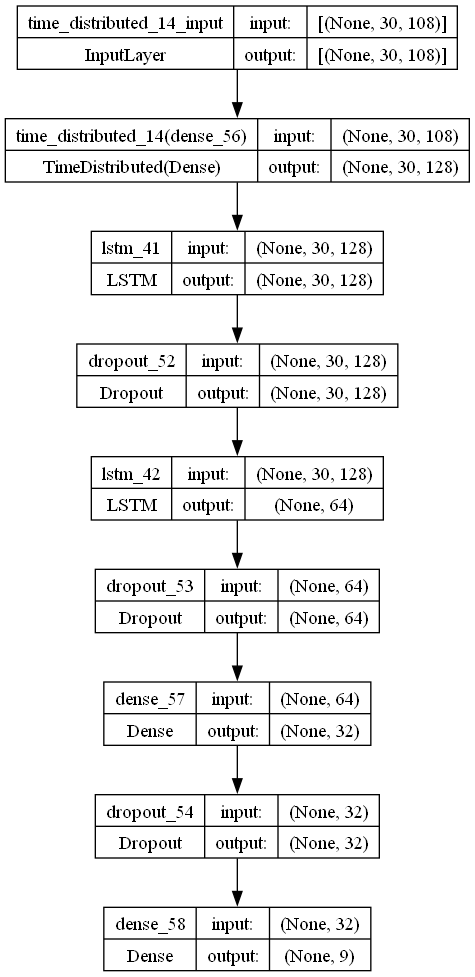
\includegraphics[scale=0.5]{gambar/bab4-uji-model-best-model.png}

  \caption{Model LSTM}
  \label{fig:modelLSTM}
\end{figure}

\subsection{Sistem Kontrol}
\label{sec:metodologisistemkontrol}

Adapun dalam pembuatan tugas akhir ini, sistem kontrol adalah serangkaian proses yang akan mengatur bagaimana nantinya bahasa isyarat akan dideteksi, melakukan penanggulangan terhadap adanya kesalahan pendeteksian, menyatukan berbagai kata dalam bentuk kalimat, penghapusan kosakata, dan penerjemahan kalimat dalam bentuk suara. Penggunaan sistem kontrol ini diharapkan akan memudahkan pengguna dalam menggunakan program penerjemah bahasa isyarat Indonesia (BISINDO). Sistem kontrol akan dibagi menjadi 2, yaitu program deteksi bahasa isyarat dan program pembentukan kalimat.

\subsubsection{Program Deteksi Bahasa Isyarat}

\begin{figure}[H]
  \centering

  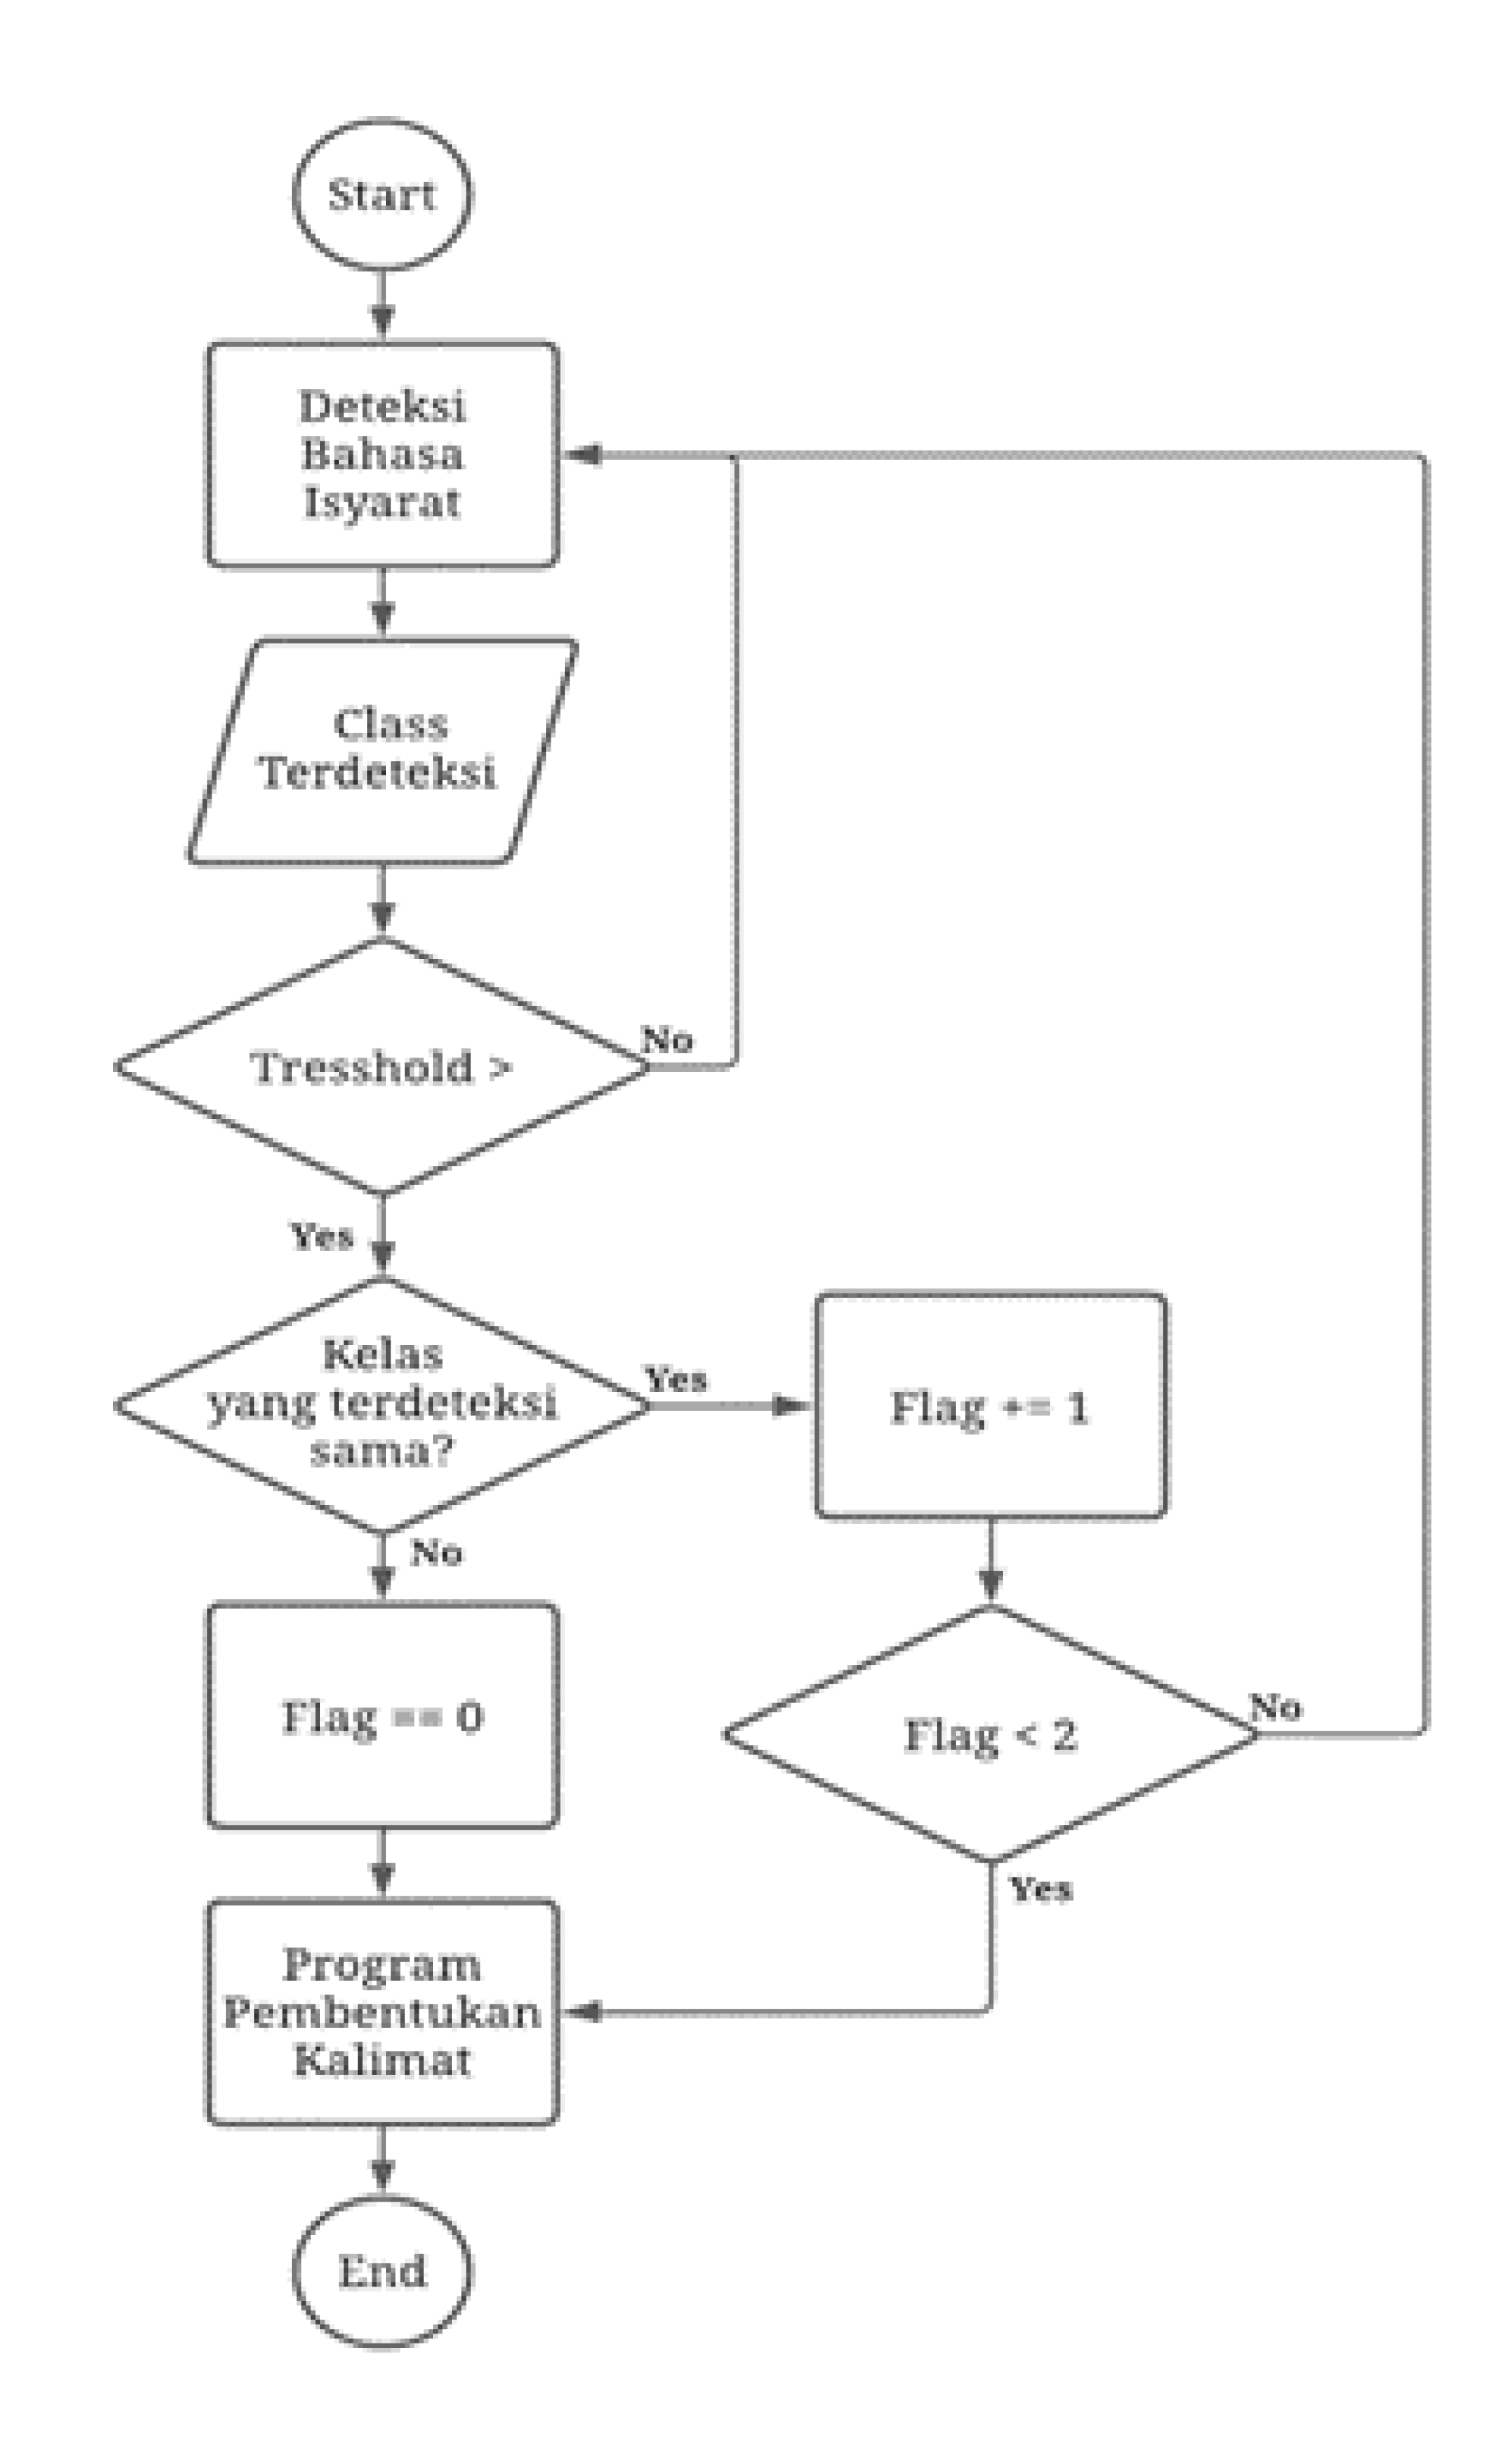
\includegraphics[scale=0.54]{gambar/bab3-flowchart-deteksi.png}

  \caption{Flowchart program deteksi bahasa isyarat}
  \label{fig:flowchartdeteksi}
\end{figure}
Pada program deteksi bahasa isyarat (dapat dilihat pada \ref{fig:flowchartdeteksi}) akan berjalan terlebih dahulu ketika pengguna terdeteksi benar memberikan isyarat start dan pengguna dapat membentuk isyarat yang diinginkan. Kemudian \textit{class} kosakata isyarat yang terdeteksi oleh model akan dipastikan apakah melebihi \textit{threshold} atau ambang batas yang telah ditentukan untuk menghindari adanya kesalahan pembacaan (\textit{error}) dan \textit{noise} dalam pembacaan bahasa isyarat. Apabila dibawah dari \textit{threshold}, maka program akan melakukan pendeteksian kembali bahasa isyarat dari pengguna. Apabila benar diatas dari \textit{threshold} yang ditentukan, maka akan diperiksa apakah \textit{class} yang terdeteksi sama dengan \textit{class} sebelumnya. Apabila terdeteksi sama maka nilai \textit{flag} akan ditambah 1. Nilai \textit{flag} akan diperiksa apakah kurang dari 2, apabila salah maka akan kembali untuk mendeteksi bahasa isyarat dari pengguna. Hal ini dilakukan demi menghindari terjadinya pembacaan isyarat secara berulang kali. Apabila nilai \textit{flag} bernilai 1 atau 0 (nilai awal \textit{flag} adalah 0), maka akan dilanjutkan ke program pembentukan kalimat.

\subsubsection{Program Pembentuk Kalimat}
\begin{figure}[H]
  \centering

  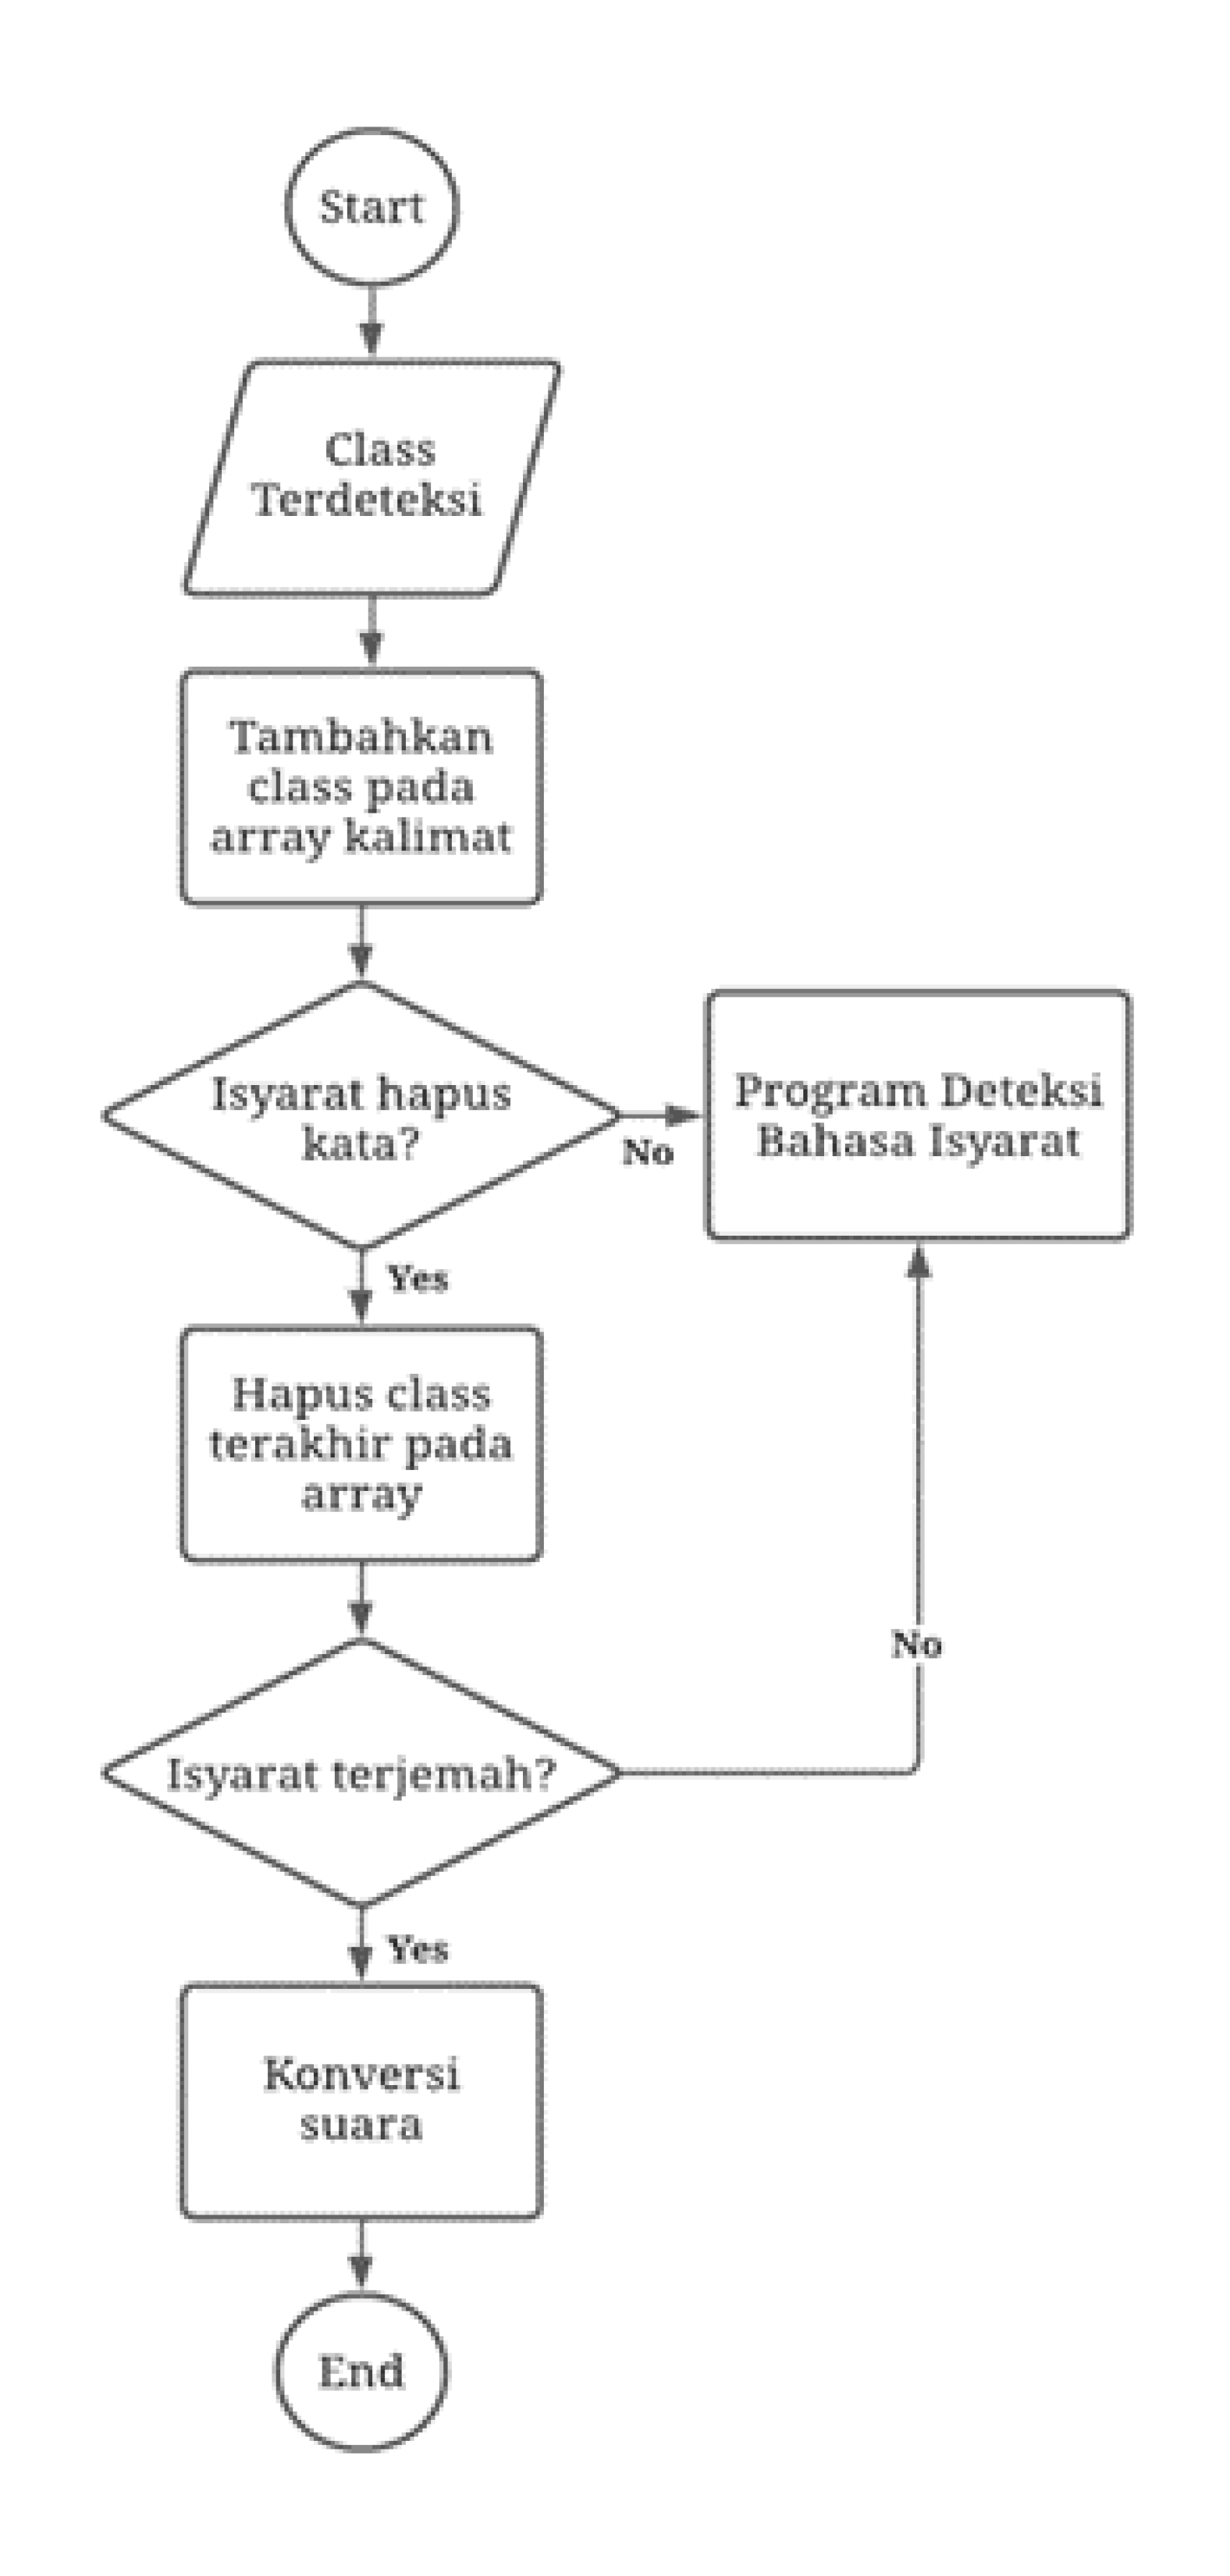
\includegraphics[scale=0.54]{gambar/bab3-flowchart-kalimat.png}

  \caption{Flowchart Program pembentukan kalimat}
  \label{fig:flowchartkalimat}
\end{figure}

Pada program pembentukan kalimat (dapat dilihat pada \ref{fig:flowchartkalimat}), terlebih dahulu \textit{class} kosakata yang terdeteksi akan dimasukkan pada suatu array kalimat dan ditambahkan spasi setelahnya. Hal ini nantinya akan memudahkan pengguna dalam membentuk kalimat yang diinginkan. Kemudian dilakukan pengecekan apakah pengguna melakukan isyarat delete atau hapus, apabila iya maka akan dilakukan penghapusan pada kata terakhir pada array. Apabila tidak maka akan dilanjutkan untuk melakukan pendeteksian bahasa isyarat selanjutnya. Dilakukan juga pengecekan apakah terdapat isyarat translate atau isyarat terjemah, jika iya maka akan dilakukan konversi dari array kalimat yang telah disimpan ke dalam suara dengan memanfaatkan \textit{library} gTTS. Library gTTS merupakan \textit{library} Python yang memiliki kemampuan untuk mengubah suatu string menjadi suara. Nantinya akan dipilih suara dengan aksen Indonesia untuk meningkatkan familiaritas terhadap lingkungan sekitar. Apabila tidak maka akan dilanjutkan untuk melakukan pendeteksian bahasa isyarat selanjutnya.

\subsection{Integrasi Intel Next Unit Computing (NUC)}
\begin{figure}[H]
  \centering

  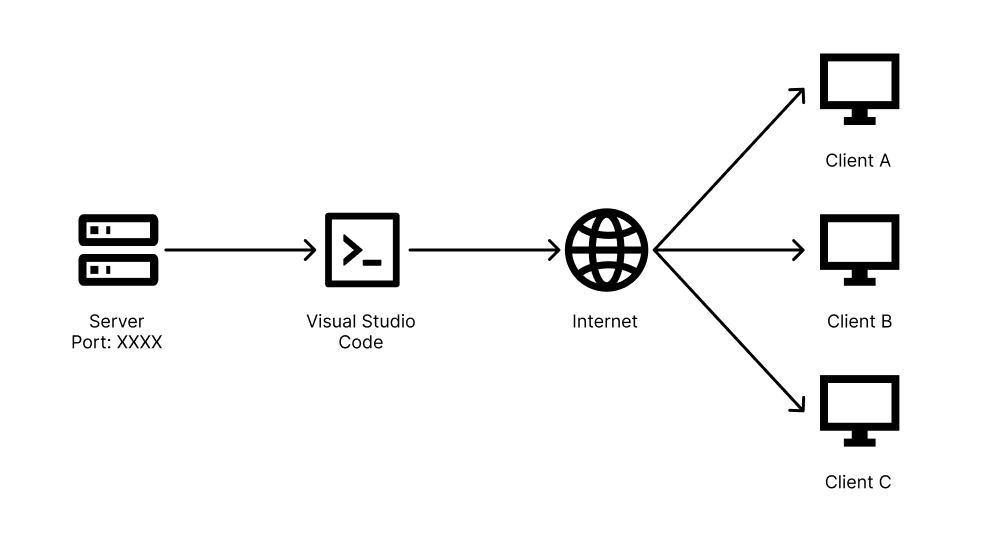
\includegraphics[scale=0.9]{gambar/bab3-path-forwarding.png}

  \caption{Skema integrasi dengan Intel NUC}
  \label{fig:diagrampathforward}
\end{figure}

Sebelum melakukan integrasi, terlebih dahulu perangkat dihubungkan dengan perangkat pendukung seperti monitor, keyboard, mouse, dan speaker. Kemudian, integrasi dengan Intel NUC dilakukan dengan mengakses website penerjemah yang telah terhubung dengan server komputer menggunakan skema \emph{port forwarding} dengan diagram alur yang dapat dilihat pada \ref{fig:blockdiagrammethod}. Server terelebih dahulu mengakses Visual Studio Code untuk menjalankan website penerjemah yang dibuat menggunakan \emph{framework} Streamlit. Akan didapatkan alamat untuk mengakses website tersebut secara lokal (\emph{localhost}), dimana nilai port yang dimiliki oleh server akan diteruskan (\emph{forwarding}) dengan bantuan Ngrok sehingga nantinya akan dapat diakses melalui internet dengan bebas oleh client, yang mana dalam hal ini adalah Intel NUC itu sendiri.

Dapat dilihat pada gambar \ref{fig:tampilanwebsite} bahwa website penerjemah akan mengakses webcam perang\\kat untuk mendapatkan data citra berbentuk video secara \emph{realtime}. Pengguna kemudian dapat melakukan gerakan bahasa isyarat BISINDO di depan webcam. Website penerjemah akan mengekstrak data citra untuk diproses melalui model LSTM yang telah dilatih sebelumnya dan melakukan penerjemahan secara \emph{realtime} sesuai dengan alur program yang telah dijelaskan sebelumnya pada sub bab \ref{sec:metodologisistemkontrol}. 

\begin{figure}[H]
  \centering

  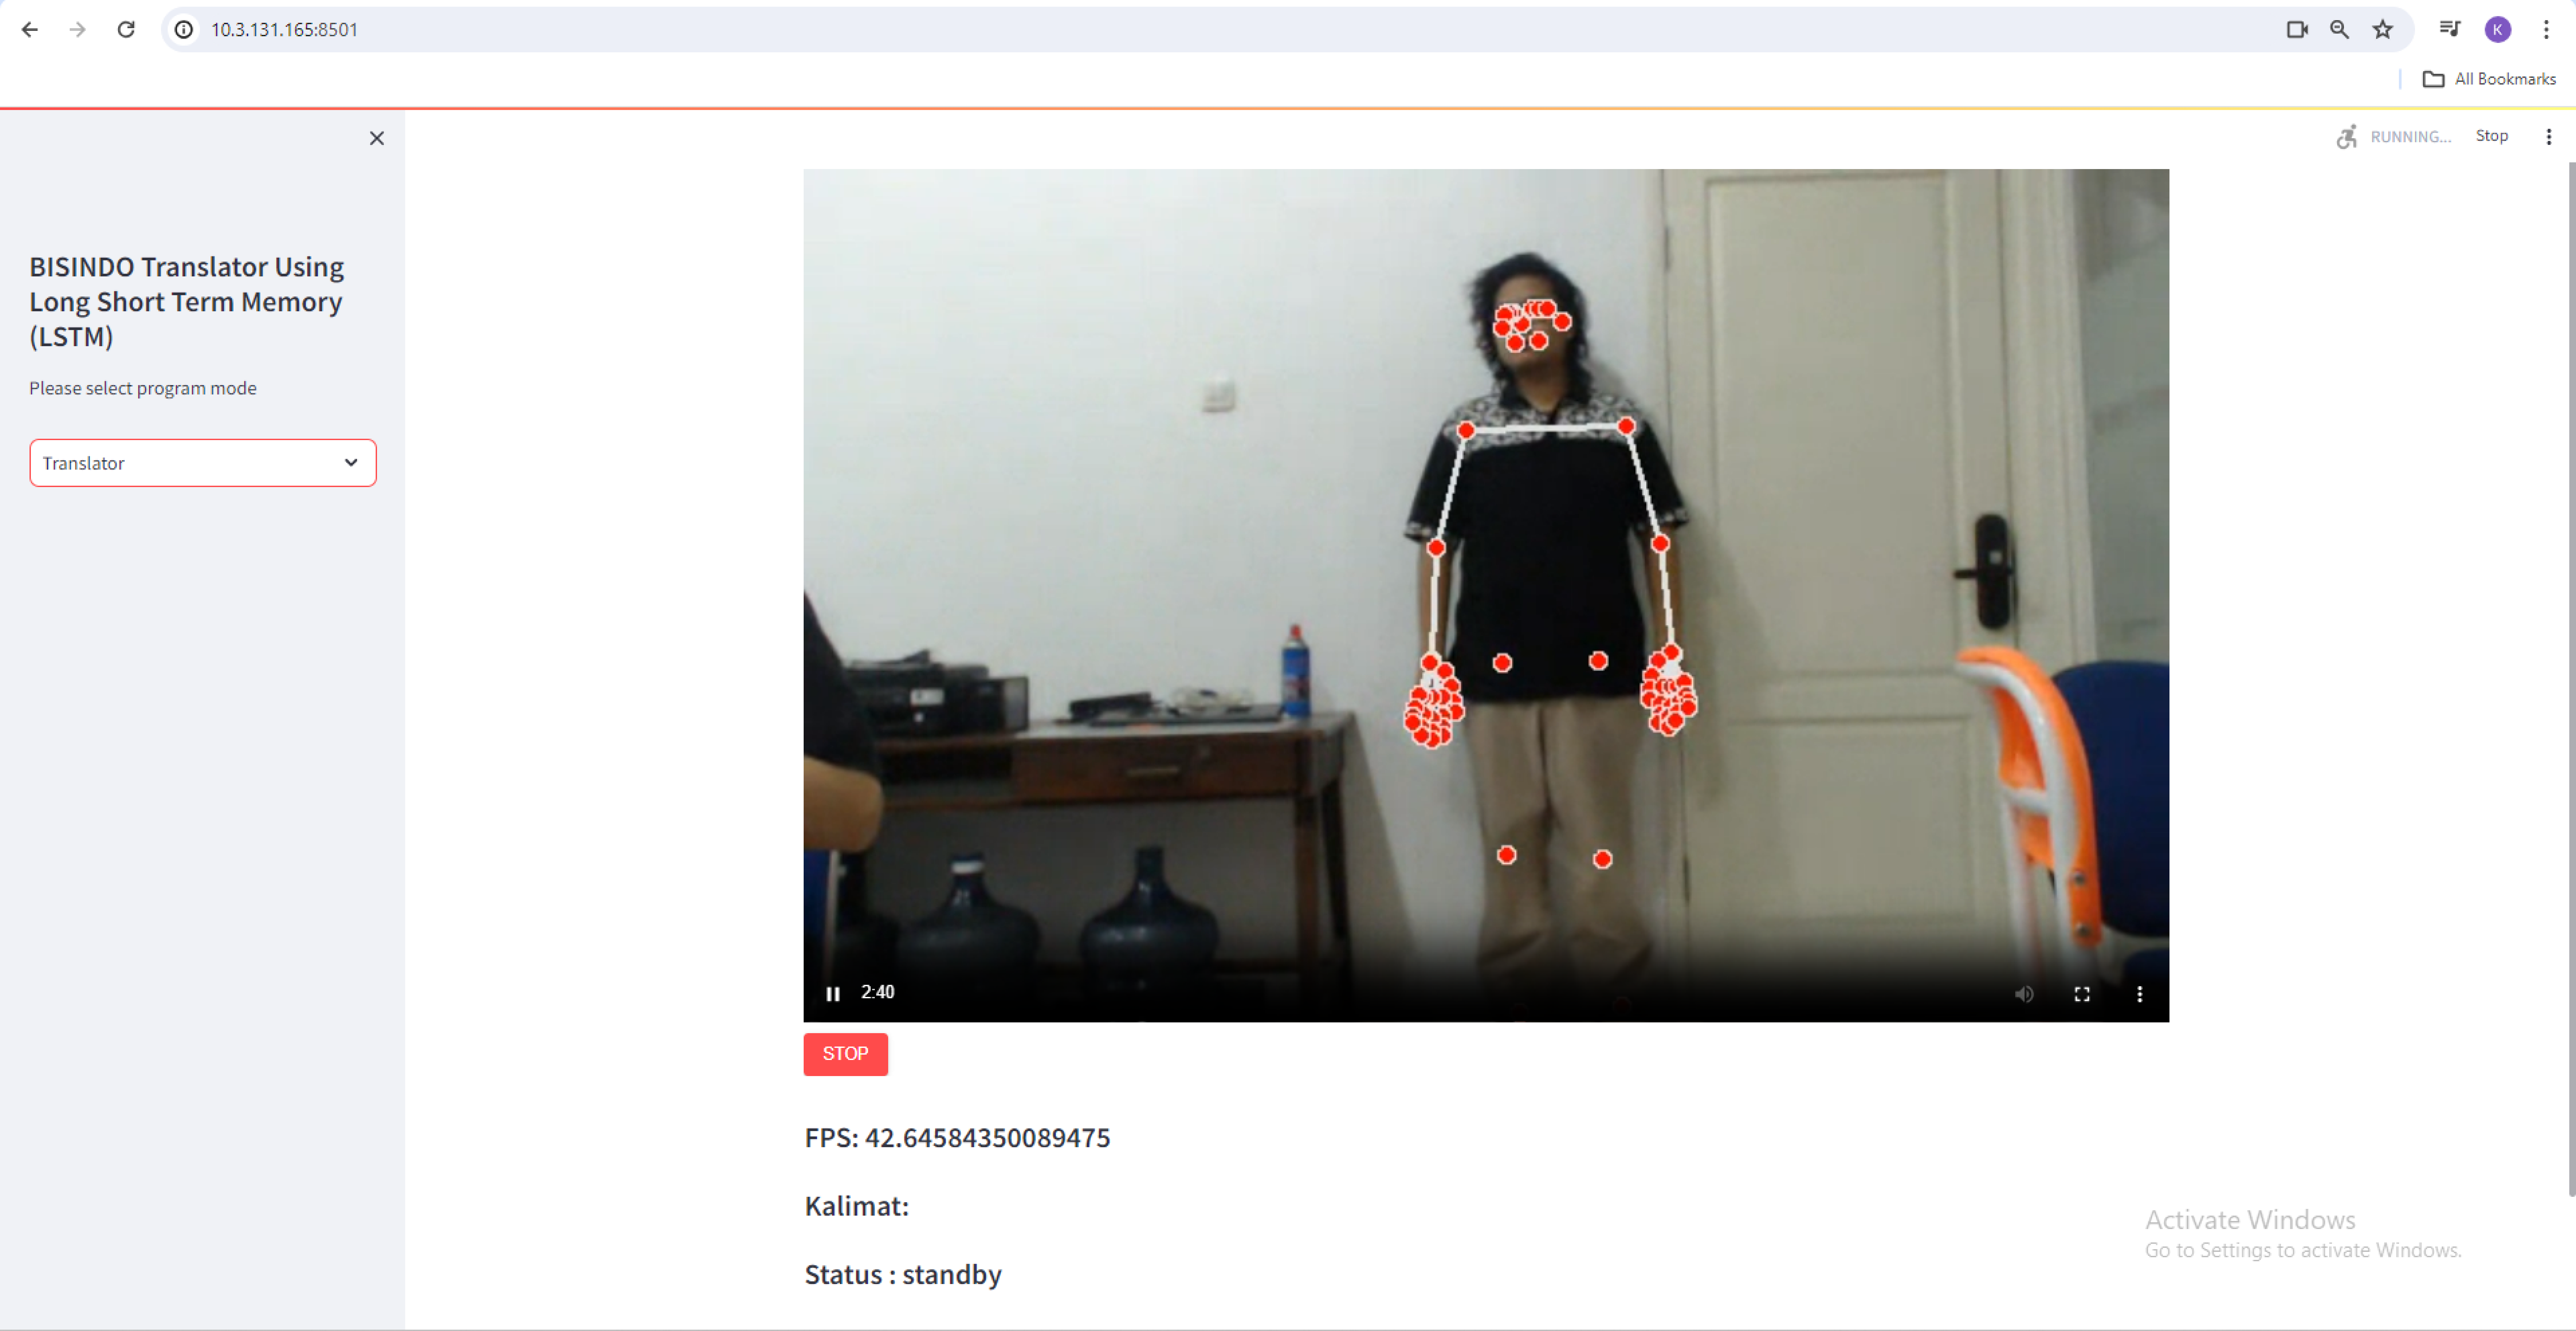
\includegraphics[scale=0.2]{gambar/bab3-layoutweb.png}

  \caption{Tampilan website}
  \label{fig:tampilanwebsite}
\end{figure}


% \subsection{Integrasi Jetson Nano}

% Sebelum dapat menggunakan Jetson Nano, terlebih dahulu mengunuh dan mengingstall NVIDIA JetPack SDK yang mencakup sistem operasi, \textit{library}, API, dan driver yang diperlukan. Proses ini melibatkan penggunaan aplikasi SDK Manager yang menyediakan antarmuka pengguna grafis untuk memudahkan penginstalan dan setup. Selanjutnya, konfigurasi perangkat keras Jetson Nano, termasuk menyediakan sumber daya listrik yang stabil, menghubungkan perangkat ke monitor melalui port HDMI, serta menyiapkan periferal lain seperti keyboard dan mouse. Untuk pengembangan yang melibatkan pengolahan citra atau video, kamera yang kompatibel juga perlu dihubungkan dan dikonfigurasi. Oleh karena Jetson Nano tidak memiliki port audio, maka digunakan USB dongle untuk dapat menyambungkan Jetson Nano dengan speaker. Kemudian dilakukan instalasi untuk setiap dependency atau \textit{library} yang dibutuhkan, seperti Python, Jupyter, TensorFlow, Keras, Pytorch, MediaPipe, Numpy, Maplotlib, dan \textit{library} lainnya. Untuk dapat menunjang performa dari Jetson Nano dalam menjalankan program, terkhususnya model penerjemah bahasa isyarat, dilakukan instalasi dan setup untuk CUDA (\textit{Compute Unified Device Architecture}) sehingga Jetson Nano dapat menggunakan GPU (\textit{Graphic Processing Unit}). 

% Untuk melakukan deploy program pendeteksi bahasa isyarat pada Jetson Nano, pada model yang telah dihasilkan sebelumnya dilakukan optimasi dengan melakukan konversi menggunakan TensorRT dan kuantisasi. Hal ini dimaksudkan untuk mengoptimalkan performa model pada Jetson Nano. Kemudian program sistem penerjemah bahasa isyarat (dalam bentuk python executable) dapat ditransfer ke Jetson Nano dengan menggunakan Git. Program siap melakukan penerjemahan bahasa isyarat BISINDO.

% \section{Urutan Pelaksanaan}

% Adapun dalam pembuatan tugas akhir ini, berikut urutan pelaksanaan penelitian yang akan dilakukan oleh penulis:

% \begin{figure}[H]
%   \centering
%   \caption{Flowchart Program Pembentukan Kalimat}
%   \label{tbl:flowchartkalimat}

%   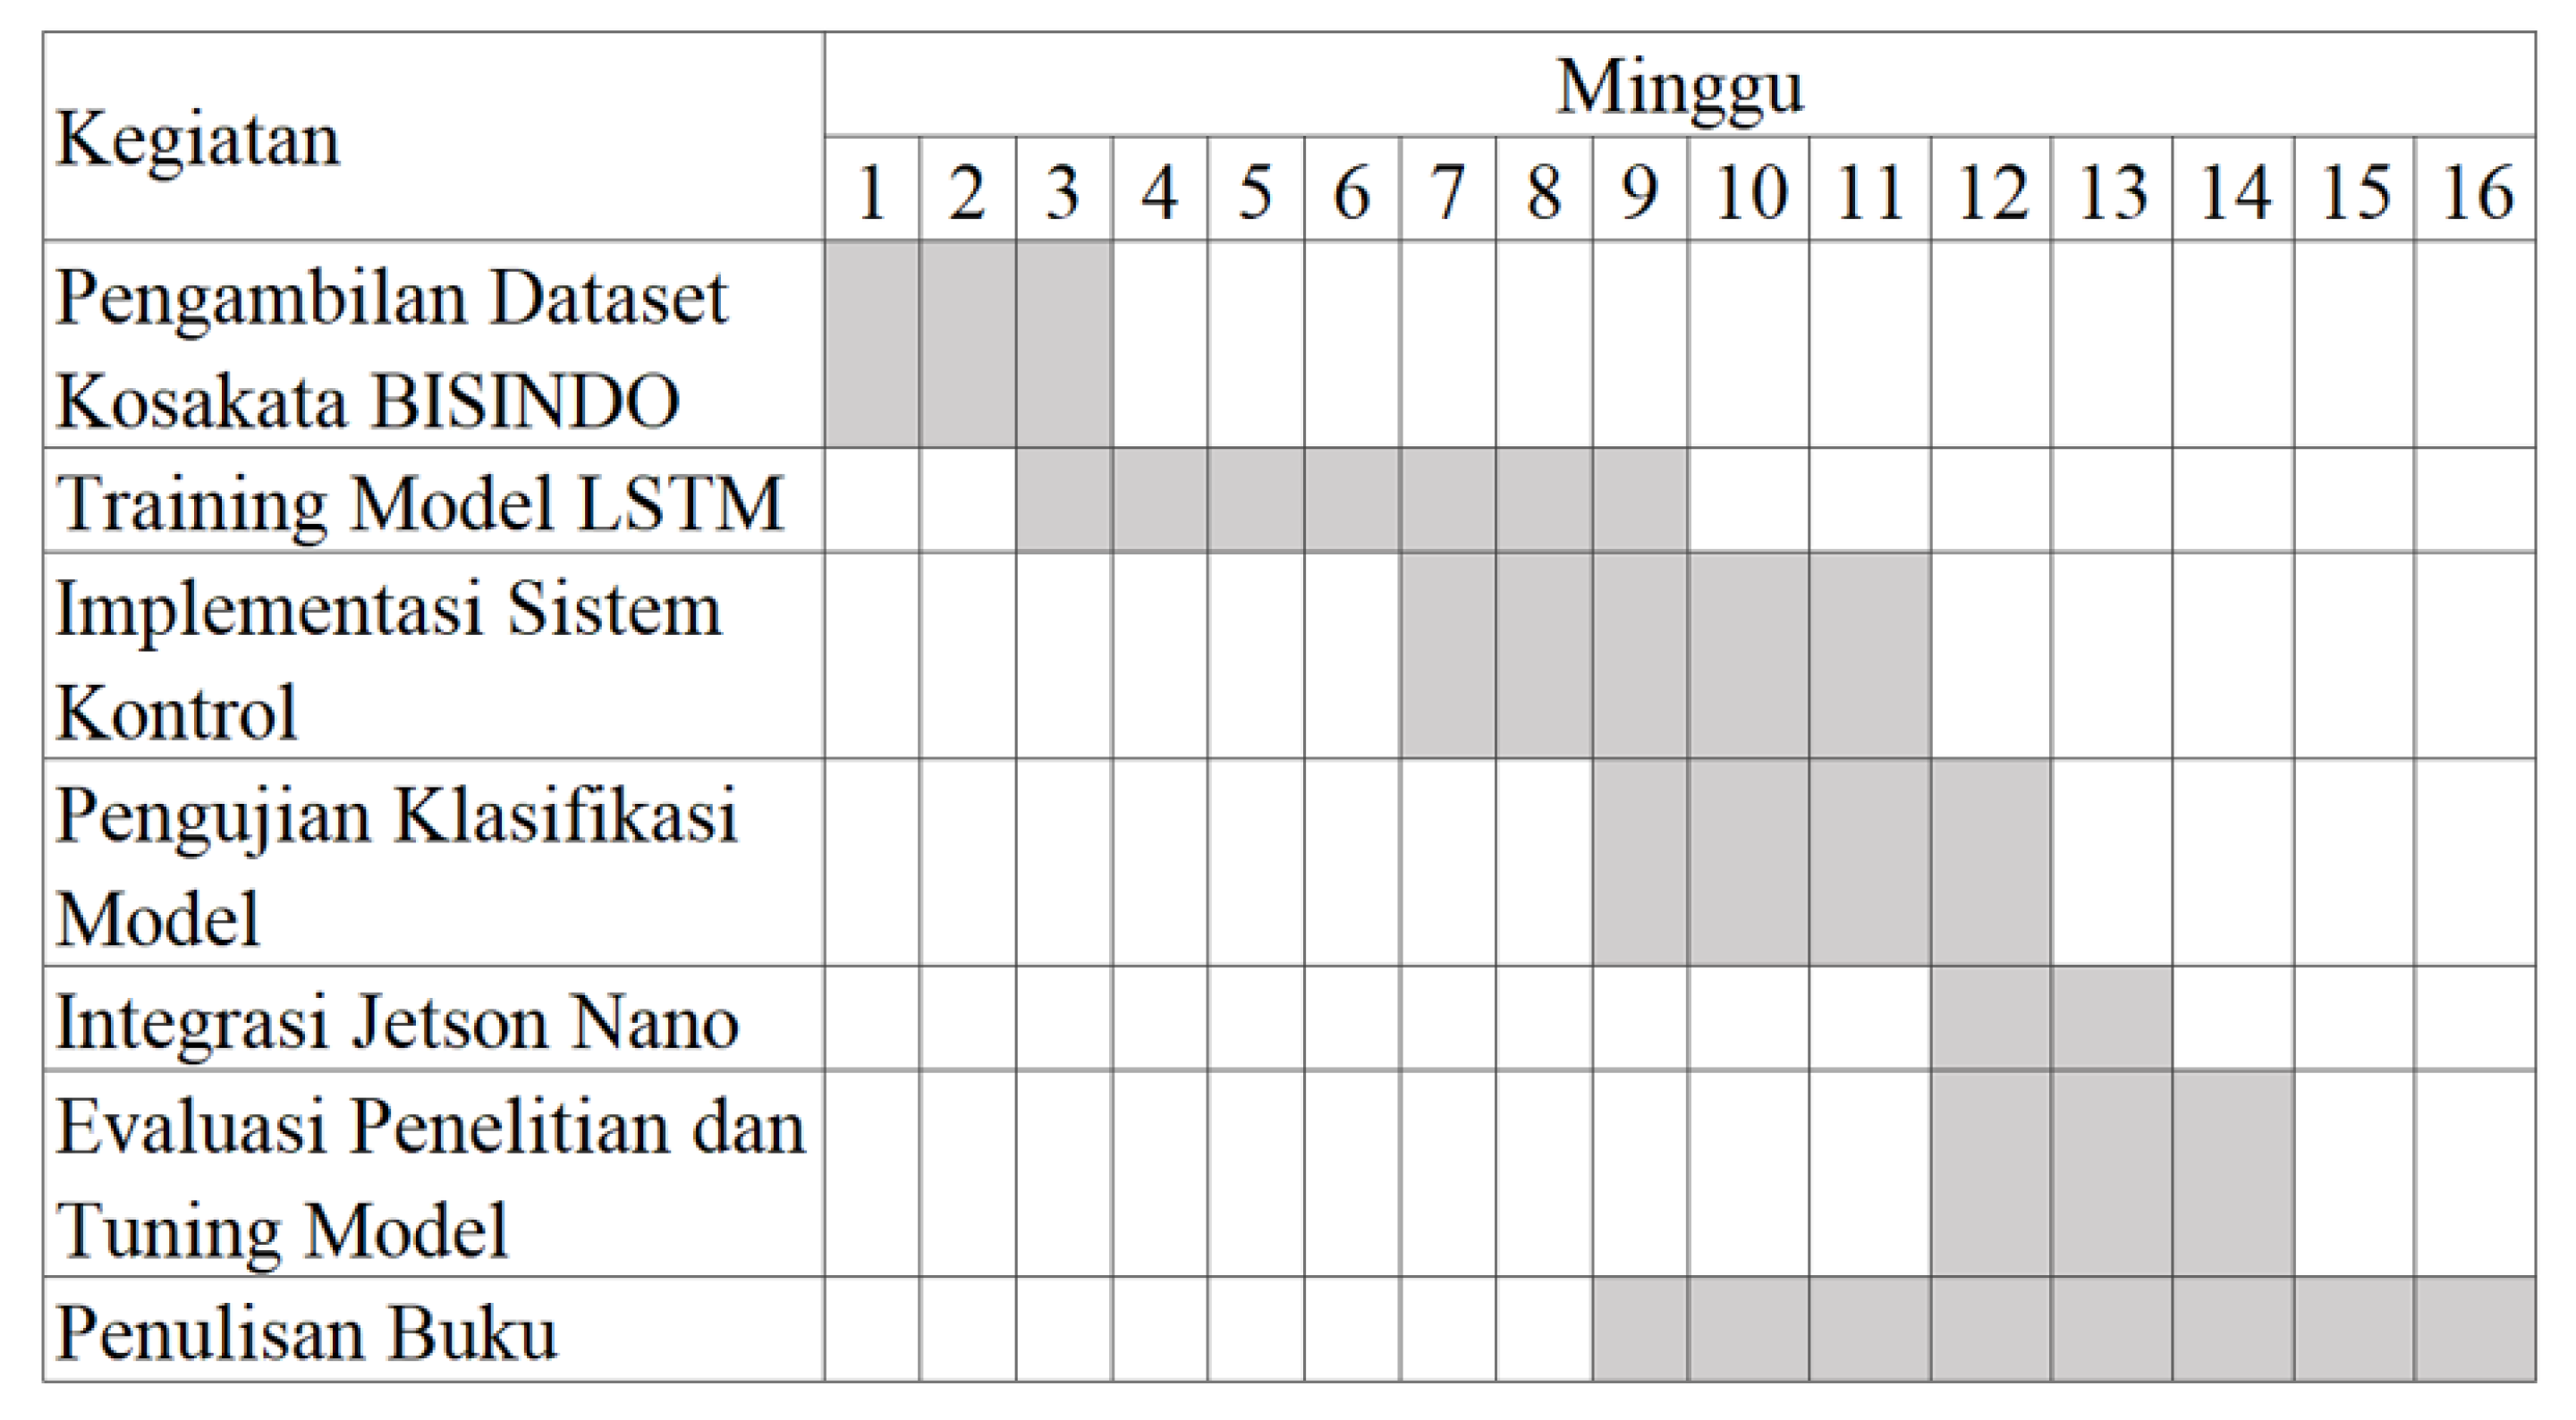
\includegraphics[scale=0.6]{gambar/bab3-timeline-kerja.png}
% \end{figure}

% \section{Deskripsi Sistem}
% \label{sec:deskripsisistem}

% Sistem akan dibuat dengan \lipsum[1-2]

% \section{Implementasi Alat
%   \label{sec:implementasi alat}}

% Alat diimplementasikan dengan \lipsum[1]

% % Contoh pembuatan potongan kode
% \begin{lstlisting}[
%   language=C++,
%   caption={Program halo dunia.},
%   label={lst:halodunia}
% ]
% #include <iostream>

% int main() {
%     std::cout << "Halo Dunia!";
%     return 0;
% }
% \end{lstlisting}

% \lipsum[2-3]

% % Contoh input potongan kode dari file
% \lstinputlisting[
%   language=Python,
%   caption={Program perhitungan bilangan prima.},
%   label={lst:bilanganprima}
% ]{program/bilangan-prima.py}

% \lipsum[4]

% \cleardoublepage

% Bab 4 pengujian dan analisis
% \chapter{PENGUJIAN DAN ANALISIS}
\label{chap:pengujiananalisis}

% Ubah bagian-bagian berikut dengan isi dari pengujian dan analisis

Pada bab ini akan dipaparkan skenario pengujian yang  dilakukan berdasarkan dari metodol\\ogi yang telah dibahas sebelumnya beserta dengan pembahasannya. Pengujian akan dilaksanakan untuk menjawab permasalahan yang diangkat sehingga dapat ditarik kesimpulan dari pelaksanaan tugas akhir ini.

\section{Skenario Pengujian}
\label{sec:skenariopengujian}

Pengujian ini akan dilakukan dengan menggunakan Intel NUC 11 Performance Kit yang telah terhubung ke internet untuk mengakses program melalui browser. Dibutuhkan juga tambahan koneksi dengan webcam eksternal sebagai media pengambilan data yang akan diproses pada program, serta keyboard, mouse, dan monitor untuk memudahkan dalam mengoperasikan program. Adapun pengujian ini akan mengikuti beberapa skenario - skenario pengujian yang ditentukan sebagai berikut:


\begin{longtable}{|c|p{8cm}|p{6cm}|}
  \caption{Skenario Pengujian}
  \label{tb:skenario}                                   \\
  \hline
  \rowcolor[HTML]{C0C0C0}
  \textbf{No.} & \multicolumn{1}{>{\centering\arraybackslash}p{8cm}|}{\textbf{Skenario Pengujian}} & \multicolumn{1}{>{\centering\arraybackslash}p{6cm}|}{\textbf{Variasi Pengujian}} \\ \hline
  1 & Skenario pengujian berdasarkan bentuk model  & 3 model yang berbeda \\ \hline
  2 & Skenario pengujian berdasarkan kondisi pencahayaan yang berbeda & Intensitas cahaya 35 lux, 80 lux, 125 lux \\ \hline
  3 & Skenario pengujian berdasarkan jarak subjek yang berbeda & Jarak 180 cm, 240 cm, 300 cm \\ \hline
  4 & Skenario pengujian dengan menggunakan subjek yang berbeda selain penulis & 1 subjek perempuan dan 1 subjek laki - laki \\ \hline
  5 & Skenario pengujian pembentukan kalimat dan konversi menjadi media suara & 3 kalimat yang dibentuk dari 3 kosakata dan 4 kalimat yang dibentuk dari 2 kosakata \\ \hline
\end{longtable} 

\section{Pengujian Bentuk Model}
\label{sec:analisismodel}

Pengujian bentuk model penerjemah bahasa isyarat Indonesia (BISINDO) dilakukan dengan melakukan perubahan struktur dari \emph{layer} yang digunakan, baik dari segi pemilihan tipe \emph{layer}, fungsi \emph{activation}, serta jumlah unit aktivasi yang digunakan. Pengujian ini didasari dari struktur model yang telah dibahas pada sub bab \ref{sec:metodologipose}. Serangkaian model yang diuji akan dilihat bagaimana performa hasil dari \emph{training} model, melalui grafik \emph{accuracy} dan \emph{loss} yang dihasilkan. Digunakan \emph{confusion matrix} untuk mengamati bagaimana hasil dari pengujian model terhadap serangkaian data gerakan bahasa isyarat dengan membandingkan hasil prediksi model dengan data aktual yang ada untuk masing - masing kosakata atau \emph{class} yang ada. Berdasarkan \emph{confusion matrix} ini juga dapat dihasilkan matrix evaluasi berupa \emph{accuracy}, \emph{precision}, \emph{recall}, dan \emph{F1-score}. Setiap model yang diuji menggunakan partisi data \emph{training} dan validasi yang sama, yaitu dengan perbandingan 70:30. Hal ini menunjukkan bahwa dari keseluruhan data yang digunakan, akan terdapat 70\% data \emph{training} dan 30\% data validasi. Untuk setiap kosakata yang digunakan sesuai dengan yang telah dijelaskan pada sub bab \ref{sec:metodologidataset}. Keseluruhan model akan dilatih sebanyak 12 \emph{epoch}. Pengujian ini bertujuan untuk melihat bagaimana perubahan struktur dari \emph{layer} akan berpengaruh pada performa model penerjemah yang dihasilkan.

\subsection{Model Pertama}
\label{sec:analisismodel1}
Model pertama menggunakan 2 buah \emph{layer} LSTM. \emph{Layer} LSTM pertama menggunakan fungsi aktivasi \emph{relu} dan dengan unit aktivasi bernilai 128 dan \emph{layer} LSTM kedua menggunakan fungsi aktivasi \emph{relu} dan dengan unit aktivasi bernilai 64. Untuk setiap \emph{layer} LSTM akan diikuti dengan \emph{layer} Dropout bernilai 0.5 untuk mencegah nilai \emph{weight} yang terlalu tinggi. Setelah serangkaian \emph{layer} LSTM, diikuti dengan \emph{layer} Dense dengan fungsi aktivasi \emph{relu} dan dengan unit aktivasi bernilai 32. Struktur lengkap dari model ini dapat dilihat pada \ref{fig:model1-struktur}.

\begin{figure}[H]
  \centering

  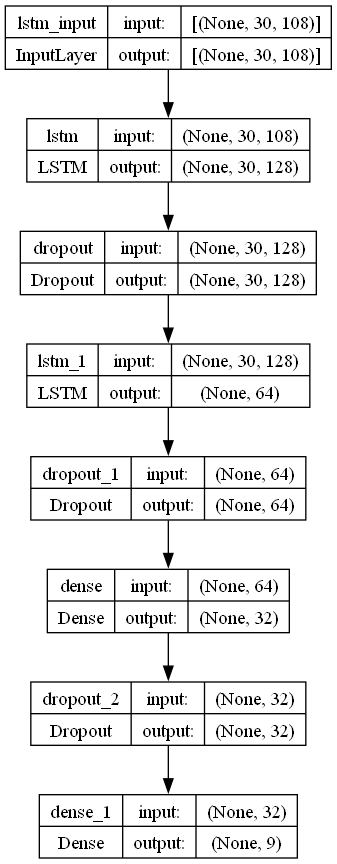
\includegraphics[scale=0.5]{gambar/bab4-uji-model-worst-model.png}

  \caption{Struktur model pertama}
  \label{fig:model1-struktur}
\end{figure}

Berdasarkan dari \emph{training} yang telah dilakukan didapatkan bahwa model menghasilkan akurasi validasi bernilai 0.89 dan akurasi \emph{training} bernilai 0.71. Data ini menunjukkan bahwa model memiliki akurasi yang cukup baik. Untuk nilai \emph{loss training} bernilai cukup tinggi, yaitu bernilai 2.81 dan \emph{loss} validasi bernilai 0.76 yang cukup rendanh jika dibandingkan dengan nilai \emph{loss training}. Nilai dari \emph{loss training} terlihat melonjak di \emph{epoch} terakhir, yaitu pada \emph{epoch} 12. Hal ini selaras dengan penurunan \emph{accuracy} model setelah \emph{epoch} 10. Grafik akurasi dan \emph{loss} dapat dilihat pada gambar \ref{fig:model1-train-acc} dan gambar \ref{fig:model1-train-loss}.

\begin{figure}[H]
  \centering

  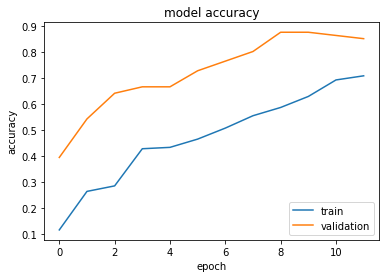
\includegraphics[scale=0.6]{gambar/bab4-uji-model-worst-acc.png}

  \caption{Hasil \emph{accuracy} model pertama}
  \label{fig:model1-train-acc}
\end{figure}

\begin{figure}[H]
  \centering

  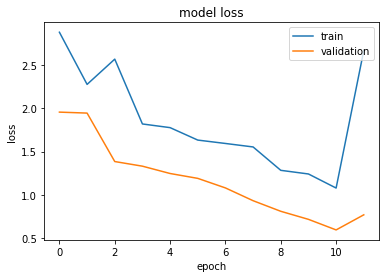
\includegraphics[scale=0.6]{gambar/bab4-uji-model-worst-loss.png}

  \caption{Hasil \emph{loss} model pertama}
  \label{fig:model1-train-loss}
\end{figure}

Kemudian berdasarkan model yang telah dihasilkan, dilakukan pengujian dengan dataset \emph{testing} yang menghasilkan \emph{confusion matrix}. Dapat dilihat pada gambar \ref{fig:model1-cf}, untuk kosakata "maaf", "tolong", "rumah", "delete", dan "translate" menghasilkan prediksi yang tepat untuk keseluruhan dataset \emph{testing} yang diujikan. Namun, kosakata "nama", "saya", "siapa", dan "standby" menghasilkan beberapa prediksi yang tidak sesuai dengan dataset \emph{testing}. Kosakata "nama" menghasilkan 6 prediksi tepat dan 4 prediksi yang kurang tepat (1 dataset \emph{testing} bernilai "siapa" dan 3 dataset \emph{testing} bernilai "rumah"). Kosakata "saya" menghasilkan 10 prediksi tepat dan 2 prediksi yang kurang tepat (dataset \emph{testing} bernilai "translate"). Kosakata "siapa" menghasilkan 3 prediksi tepat dan 5 prediksi yang kurang tepat (2 dataset \emph{testing} bernilai "tolong",  2 dataset \emph{testing} bernilai "saya", dan 1 dataset \emph{testing} bernilai "translate"). Kosakata "standby" menghasilkan 7 prediksi tepat dan 1 prediksi yang kurang tepat (dataset \emph{testing} bernilai "saya"). Adapun berdasarkan hasil \emph{confusion matrix} ini didapat matrix evaluasi berupa \emph{accuracy}, \emph{precision}, \emph{recall}, dan \emph{F1-score} yang dapat dilihat pada tabel \ref{tb:model1stat}. Rata - rata nilai \emph{accuracy} sebesar 0.85, rata - rata nilai \emph{precision} sebesar 0.85, rata - rata nilai \emph{recall} sebesar 0.85, dan rata - rata nilai \emph{F1-score} sebesar 0.83.

\begin{figure}[H]
  \centering

  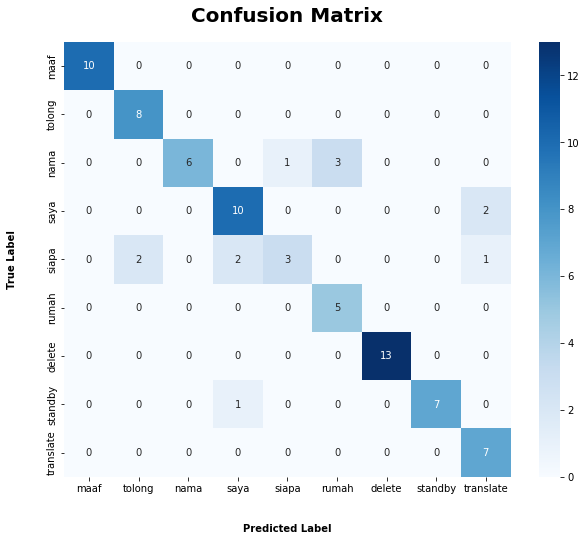
\includegraphics[scale=0.6]{gambar/bab4-uji-model-worst-cf.png}

  \caption{\emph{Confusion} model pertama}
  \label{fig:model1-cf}
\end{figure}

\begin{longtable}{|c|c|c|c|c|}
  \caption{Matrix Evaluasi Model 1}
  \label{tb:model1stat}                                   \\
  \hline
  \rowcolor[HTML]{C0C0C0}
  \textbf{Kosakata} & \textbf{\emph{Accuracy}} & \textbf{\emph{Precision}} & \textbf{\emph{Recall}} & \textbf{\emph{F1-Score}} \\
  \hline
  Maaf              & 1.00                     & 1.00                        & 1.00                   & 1.00                \\
  Tolong            & 1.00                     & 0.80                        & 1.00                   & 0.89                \\
  Nama              & 0.60                     & 1.00                        & 0.60                   & 0.75                \\
  Saya              & 0.83                     & 0.77                        & 0.83                   & 0.80                \\
  Siapa             & 0.37                     & 0.75                        & 0.38                   & 0.50                \\
  Rumah             & 1.00                     & 0.62                        & 1.00                   & 0.77                \\
  Delete            & 1.00                     & 1.00                        & 1.00                   & 1.00                \\
  Standby           & 0.87                     & 1.00                        & 0.88                   & 0.93                \\
  Translate         & 1.00                     & 0.70                        & 1.00                   & 0.82                \\
  \hline
\end{longtable}

\subsection{Model Kedua}
\label{sec:analisismodel2}

Model kedua diawali dengan \emph{layer} \textit{TimeDistributed} yang di dalamnya terdapat \emph{layer} \textit{Dense} dengan fungsi aktivasi '\textit{tanh}' dan unit aktivasi bernilai 128. Kemudian dilanjutkan dengan 1 buah \emph{layer} LSTM yang menggunakan fungsi aktivasi \emph{tanh} dan dengan unit aktivasi bernilai 64. \emph{Layer} LSTM akan diikuti dengan \emph{layer} Dropout bernilai 0.5 untuk mencegah nilai \emph{weight} yang terlalu tinggi. Setelah serangkaian \emph{layer} LSTM, diikuti dengan \emph{layer} Dense dengan fungsi aktivasi \emph{relu} dan dengan unit aktivasi bernilai 32. Struktur lengkap dari model ini dapat dilihat pada \ref{fig:model2-struktur}.

\begin{figure}[H]
  \centering

  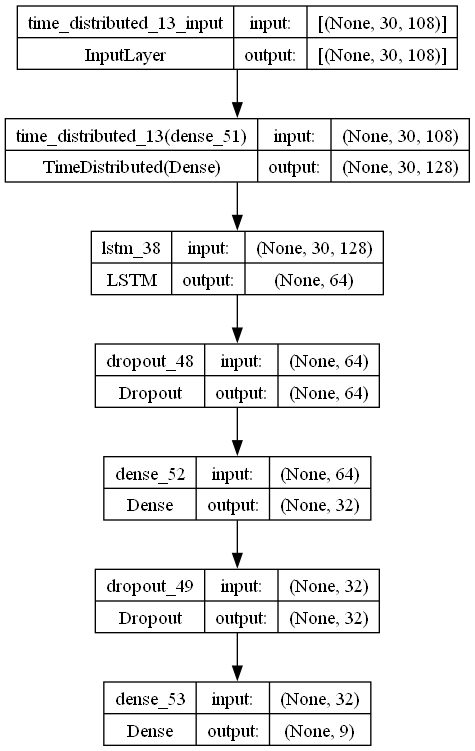
\includegraphics[scale=0.6]{gambar/bab4-uji-model-second-model.png}

  \caption{Struktur model kedua}
  \label{fig:model2-struktur}
\end{figure}

Berdasarkan dari \emph{training} yang telah dilakukan didapatkan bahwa model menghasilkan akurasi \emph{training} bernilai 0.96 dan akurasi validasi bernilai 0.93. Data ini menunjukkan bahwa model memiliki akurasi yang baik. Terdapat penurunan pada akurasi validasi pada \emph{epoch} terakhir, tetapi kebalikannya untuk akurasi \emph{training} mengalami kenaikan melebihi akurasi validasi. Untuk nilai \emph{loss training} bernilai 0.32 dan \emph{loss} validasi bernilai 0.25 yang cukup rendah jika dibandingkan dengan nilai \emph{loss training}. Data ini menunjukkan bahwa model memiliki \emph{error} prediksi yang kecil. Grafik akurasi dan \emph{loss} dapat dilihat pada gambar \ref{fig:model2-train-acc} dan gambar \ref{fig:model2-train-loss}.

\begin{figure}[H]
  \centering

  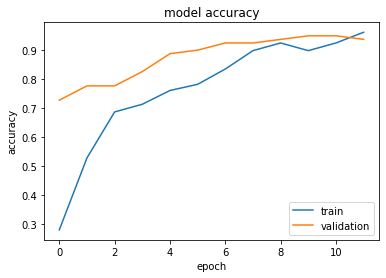
\includegraphics[scale=0.6]{gambar/bab4-uji-model-second-acc.png}

  \caption{Hasil \emph{accuracy} model kedua}
  \label{fig:model2-train-acc}
\end{figure}

\begin{figure}[H]
  \centering

  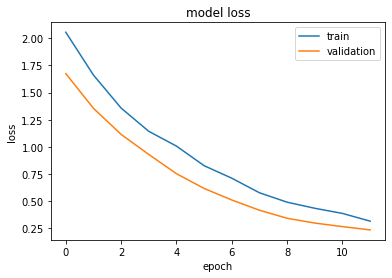
\includegraphics[scale=0.6]{gambar/bab4-uji-model-second-loss.png}

  \caption{Hasil \emph{loss} model kedua}
  \label{fig:model2-train-loss}
\end{figure}


Kemudian berdasarkan model yang telah dihasilkan, dilakukan pengujian dengan dataset \emph{testing} yang menghasilkan \emph{confusion matrix}. Dapat dilihat pada gambar \ref{fig:model2-cf}, untuk kosakata "tolong", "nama", "rumah", "delete", dan "translate" menghasilkan prediksi yang tepat untuk keseluruhan dataset \emph{testing} yang diujikan. Namun, kosakata "saya", "siapa", dan "standby" menghasilkan beberapa prediksi yang tidak sesuai dengan dataset \emph{testing}. Kosakata "maaf" menghasilkan 10 prediksi tepat dan 1 prediksi yang kurang tepat (dataset \emph{testing} bernilai "standb\\y"). Kosakata "saya" menghasilkan 11 prediksi tepat dan 2 prediksi yang kurang tepat (dataset \emph{testing} bernilai "siapa"). Kosakata "siapa" menghasilkan 5 prediksi tepat dan 1 prediksi yang kurang tepat (dataset \emph{testing} bernilai "saya"). Kosakata "standby" menghasilkan 7 prediksi tepat dan 1 prediksi yang kurang tepat (dataset \emph{testing} bernilai "siapa"). Dapat dilihat bahwa terdapat peningkatan performa dari model pertama dengan model kedua. Kosakata yang berhasil diprediksi sesuai dengan dataset \emph{testing} yang digunakan lebih banyak dibandingkan dengan model sebelumnya, yaitu 5 kosakata. Peningkatan ini disebabkan karena perubahan struktur dari model dengan adanya penggunaan \emph{layer Time Distributed} yang di dalamnya diisi dengan \emph{layer} Dense di lapisan awal model. Pengurangan pengunaan 1 \emph{layer} LSTM dapat dengan menggunakan fungsi aktivasi \emph{tanh}. Adapun berdasarkan \emph{confusion matrix} ini didapat matrix evaluasi berupa \emph{accuracy}, \emph{precision}, \emph{recall}, dan \emph{F1-score} yang dapat dilihat pada tabel \ref{tb:model2stat}. Rata - rata nilai \emph{accuracy} sebesar 0.93, nilai \emph{precision} sebesar 0.95, rata - rata nilai \emph{recall} sebesar 0.94, dan rata - rata nilai \emph{F1-score} sebesar 0.94. Dapat dilihat berdasarkan matrix evaluasi ini, terdapat peningkatan performa pada model kedua jika dibandingkan dengan model pertama. 

\begin{figure}[H]
  \centering

  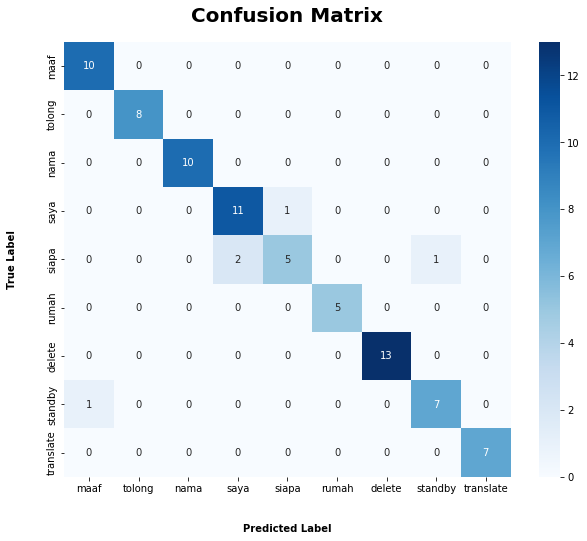
\includegraphics[scale=0.55]{gambar/bab4-uji-model-second-cf.png}

  \caption{\emph{Confusion} model kedua}
  \label{fig:model2-cf}
\end{figure}

\begin{longtable}{|c|c|c|c|c|}
  \caption{Matrix Evaluasi Model 2}
  \label{tb:model2stat}                                   \\
  \hline
  \rowcolor[HTML]{C0C0C0}
  \textbf{Kosakata} & \textbf{\emph{Accuracy}} & \textbf{\emph{Precision}} & \textbf{\emph{Recall}} & \textbf{\emph{F1-Score}} \\
  \hline
  Maaf              & 1.00                        & 0.91                        & 1.00                   & 0.95                \\
  Tolong            & 1.00                        & 1.00                        & 1.00                   & 1.00                \\
  Nama              & 1.00                        & 1.00                        & 1.00                   & 1.00                \\
  Saya              & 0.91                        & 0.85                        & 0.92                   & 0.88                \\
  Siapa             & 0.62                        & 0.93                        & 0.62                   & 0.71                \\
  Rumah             & 1.00                        & 1.00                        & 1.00                   & 1.00                \\
  Delete            & 1.00                        & 1.00                        & 1.00                   & 1.00                \\
  Standby           & 0.87                        & 0.88                        & 0.88                   & 0.88                \\
  Translate         & 1.00                        & 1.00                        & 1.00                   & 1.00                \\
  \hline
\end{longtable}

\subsection{Model Ketiga}
\label{sec:analisismodel3}

\begin{figure}[H]
  \centering

  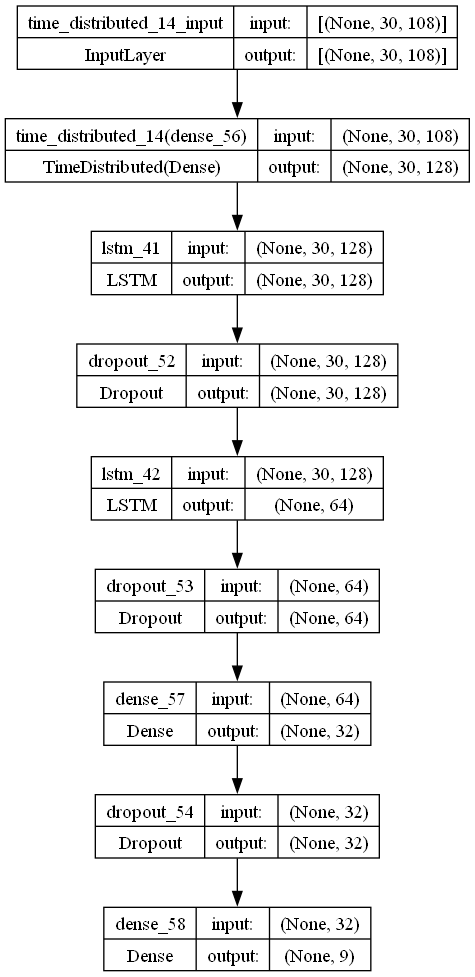
\includegraphics[scale=0.6]{gambar/bab4-uji-model-best-model.png}

  \caption{Struktur model ketiga}
  \label{fig:model3-struktur}
\end{figure}

Model ketiga merupakan gabungan dari struktur antara model 1 dan model 2. Model ini diawali dengan layer pertama berupa \emph{layer} \textit{TimeDistributed} yang di dalamnya terdapat \emph{layer} \textit{Dense} dengan fungsi aktivasi '\textit{tanh}' dan unit aktivasi bernilai 128. Selanjutnya diikuti dengan 2 buah \emph{layer} LSTM. \emph{Layer} LSTM pertama menggunakan fungsi aktivasi \emph{tanh} dengan unit aktivasi bernilai 128 dan \emph{Layer} LSTM kedua menggunakan fungsi aktivasi \emph{tanh} dengan unit aktivasi bernilai 64. Kedua \emph{layer} LSTM ini diikuti dengan \emph{layer} Dropout bernilai 0.5 untuk mencegah nilai \emph{weight} yang terlalu tinggi. Dilanjutkan dengan \emph{layer} Dense dengan fungsi aktivasi \emph{relu} dan unit aktivasi bernilai 32. Struktur lengkap dari model ini dapat dilihat pada gambar \ref{fig:model3-struktur}

\begin{figure}[H]
  \centering

  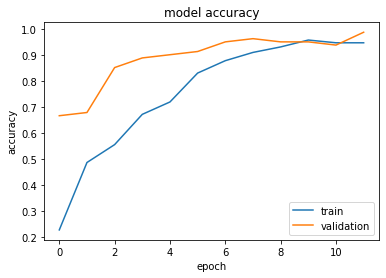
\includegraphics[scale=0.75]{gambar/bab4-uji-model-best-acc.png}

  \caption{Hasil \emph{accuracy} model ketiga}
  \label{fig:model3-train-acc}
\end{figure}

\begin{figure}[H]
  \centering

  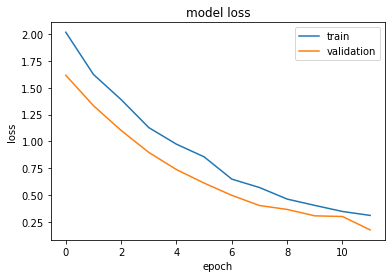
\includegraphics[scale=0.75]{gambar/bab4-uji-model-best-loss.png}

  \caption{Hasil \emph{loss} model ketiga}
  \label{fig:model3-train-loss}
\end{figure}

Berdasarkan dari \emph{training} yang telah dilakukan didapatkan bahwa model menghasilkan akurasi \emph{training} bernilai 0.94 dan akurasi validasi bernilai 1.00. Data ini menunjukkan bahwa model memiliki akurasi yang sangat baik. Untuk nilai \emph{loss training} bernilai 0.3 dan \emph{loss} validasi bernilai 0.16 yang rendah jika dibandingkan dengan nilai \emph{loss training}. Data ini menunjukkan bahwa model memiliki \emph{error} prediksi yang kecil. Hasil dari \emph{training} model ini menunjukkan bahwa model telah dapat mempelajari dataset dengan baik. Ketika dilakukan pengujian dengan menggunakan data validasi, dapat dilihat bahwa model memiliki akurasi yang lebih tinggi dan tingkat \emph{loss} yang lebih rendah dibandingkan dengan pengujian yang menggunakan data \emph{training} itu sendiri. Grafik akurasi dan \emph{loss} dapat dilihat pada gambar \ref{fig:model3-train-acc} dan gambar \ref{fig:model3-train-loss}.


Kemudian berdasarkan model yang telah dihasilkan, dilakukan pengujian dengan dataset \emph{testing} yang menghasilkan \emph{confusion matrix}. Dapat dilihat pada gambar \ref{fig:model3-cf}, untuk kosakata "maaf", "tolong", "nama", "saya",  menghasilkan prediksi yang tepat untuk keseluruhan dataset \emph{testing} yang diujikan. Namun, pada kosakata "siapa" menghasilkan beberapa prediksi yang tidak sesuai dengan dataset \emph{testing}. Kosakata "siapa" menghasilkan 7 prediksi tepat dan 1 prediksi yang kurang tepat (dataset \emph{testing} bernilai "saya"). Dapat dilihat bahwa terdapat peningkatan performa dari model ketiga dibandingkan dengan model pertama dan kedua. Peningkatan ini disebabkan karena perubahan struktur dari model dengan penggunaan \emph{layer Time Distributed} yang didalamnya diisi dengan \emph{layer} Dense di lapisan awal model. Kemudian dilanjutkan dengan 2 buah \emph{layer} LSTM yang menggunakan fungsi aktivasi \emph{tanh} Adapun berdasarkan \emph{confusion matrix} ini didapat matrix evaluasi berupa \emph{accuracy}, \emph{precision}, \emph{recall}, dan \emph{F1-score} yang dapat dilihat pada tabel \ref{tb:model3stat}. Rata - rata nilai \emph{accuracy} sebesar 0.99, rata - rata nilai \emph{precision} sebesar 0.99 rata - rata nilai \emph{recall} sebesar 0.98, dan rata - rata nilai \emph{F1-score} sebesar 0.99. Dapat dilihat berdasarkan matrix evaluasi ini, terdapat peningkatan performa pada model ketiga jika dibandingkan dengan model pertama dan kedua.

\begin{figure}[H]
  \centering

  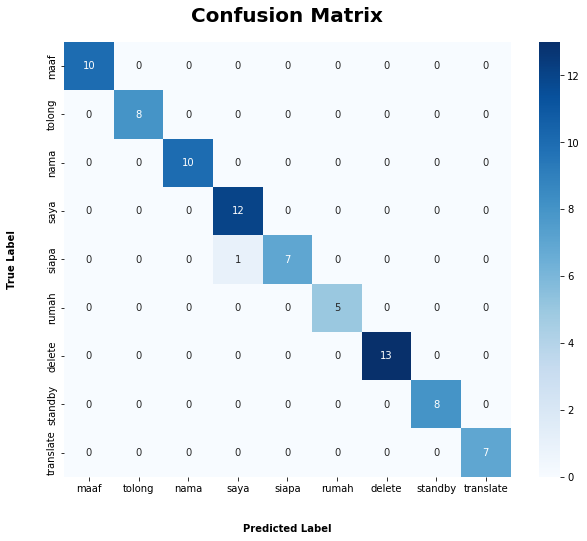
\includegraphics[scale=0.6]{gambar/bab4-uji-model-best-cf.png}

  \caption{\emph{Confusion} model ketiga}
  \label{fig:model3-cf}
\end{figure}

\begin{longtable}{|c|c|c|c|c|c|}
  \caption{Matrix Evaluasi Model 3}
  \label{tb:model3stat}                                   \\
  \hline
  \rowcolor[HTML]{C0C0C0}
  \textbf{Kosakata} & \textbf{\emph{Accuracy}} & \textbf{\emph{Precision}} & \textbf{\emph{Recall}} & \textbf{\emph{F1-Score}} \\
  \hline
  Maaf              & 1.00                       & 1.00                        & 1.00                   & 1.00                \\
  Tolong            & 1.00                       & 1.00                        & 1.00                   & 1.00                \\
  Nama              & 1.00                       & 1.00                        & 1.00                   & 1.00                \\
  Saya              & 1.00                       & 0.92                        & 1.00                   & 0.96                \\
  Siapa             & 0.87                       & 1.00                        & 0.82                   & 0.93                \\
  Rumah             & 1.00                       & 1.00                        & 1.00                   & 1.00                \\
  Delete            & 1.00                       & 1.00                        & 1.00                   & 1.00                \\
  Standby           & 1.00                       & 1.00                        & 1.00                   & 1.00                \\
  Translate         & 1.00                       & 1.00                        & 1.00                   & 1.00                \\
  \hline
\end{longtable}

\subsection{Rangkuman Pengujian Bentuk Model}
\label{sec:analisismodelseluruh}

\begin{longtable}{|c|c|c|c|c|}
  \caption{Rangkuman Pengujian Bentuk Model}
  \label{tb:evaluasiModel}                                   \\
  \hline
  \rowcolor[HTML]{C0C0C0}
  \textbf{Model} & \emph{\textbf{Avg. Accuracy}} & \emph{\textbf{Avg. Precision}} & \emph{\textbf{Avg. Recall}} & \emph{\textbf{Avg. F1-Score}} \\
  \hline
  Model 1 & 0.85 & 0.85 & 0.85 & 0.83 \\
  Model 2 & 0.93 & 0.95 & 0.94 & 0.94 \\
  Model 3 & 0.99 & 0.99 & 0.98 & 0.99 \\
  \hline
\end{longtable}

Secara keseluruhan, berdasarkan tabel \ref{tb:evaluasiModel} bahwa seiring denagn peningkatan kompleksitas dari suatu model selaras dengan peningkatan performa dari model itu sendiri. Hal ini dapat ditunjukkan dengan peningkatan akurasi dari model 1, yaitu 0.85 atau 85\% menjadi pada model 3, yaitu 0.99 atau 99\%. Nilai \emph{average precision}, {average recall},dan \emph{average F1-Score} juga meningkat seiring dengan peningkatan stuktur dari model. Penggunaan \emph{layer TimeDistributed} dan diikuti 2 \emph{layer} LSTM menghasilkan model dengan performa terbaik.

Adapun pada setiap \emph{class} yang ada menunjukkan bahwa performa kosakata 'siapa' menghasilkan hasil klasifikasi yang kurang baik. Hal ini dapat dipengaruhi oleh adanya kempiripan antara kosakata ini dengan berbagai kosakata lainnya. Pergerakan isyarat kosakata 'siapa' berfokus pada gerakan tangan yang mengarah ke depan subjek. Gerakan ini mengutamakan kedinamisan antara koordinat y yang berubah seiring dengan pergerakan tangan. Kosakata 'saya' juga memiliki fokus gerakan isyarat yang secara garis besar sama, yaitu gerakan tangan yang mengarah ke depan subjek. Hal ini menyebabkan model kesulitan dalam memberikan klasifikasi yang tepat dan cenderung \emph{overfitting} pada kosakata 'saya'. Apabila dilihat dari peresebaran kooridnat yang ada, didapat bahwa koordinat kosakata 'saya' dan 'siapa' memiliki lingkup persebaran yang hampir sama yang dapat dilihat pada gambar \ref{fig:isyarat-coor-saya} dan gambar \ref{fig:isyarat-coor-siapa}, dimana terdapat 3 'daerah' persebaran yang hampir sama. 



\begin{figure}[H]
  \centering

  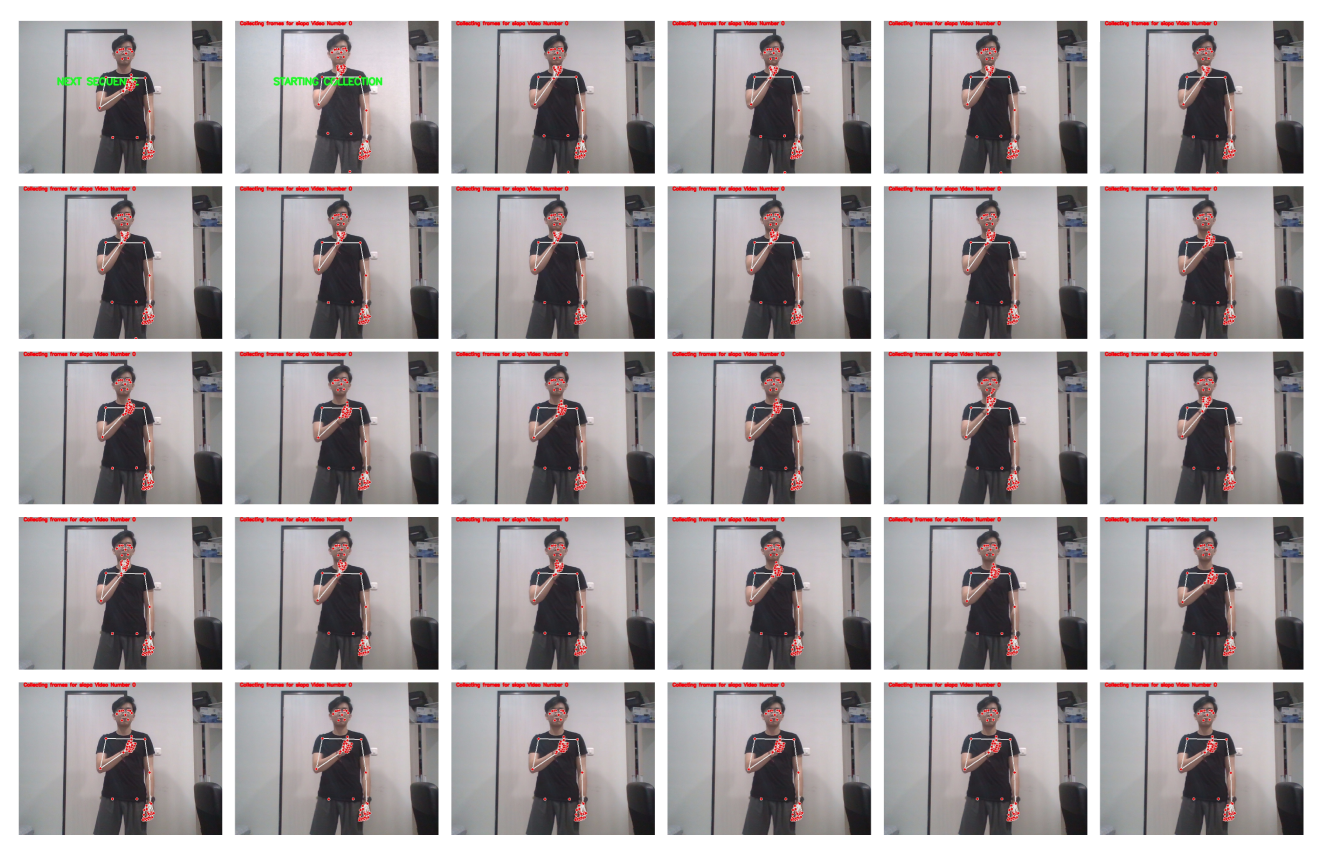
\includegraphics[scale=0.45]{gambar/isyarat-siapa.png}

  \caption{Isyarat kosakata 'siapa'}
  \label{fig:isyarat-siapa}
\end{figure}

\begin{figure}[H]
  \centering

  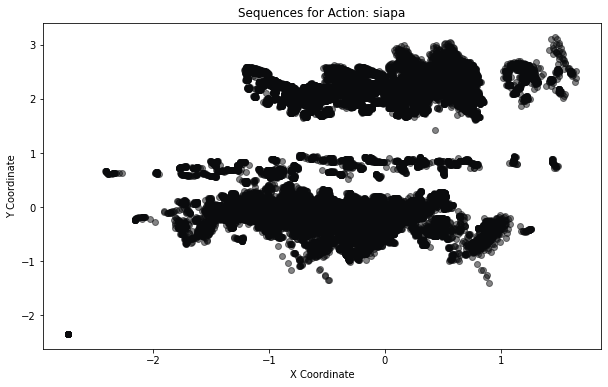
\includegraphics[scale=0.7]{gambar/coor-siapa.png}

  \caption{Persebaran koordinat kosakata 'siapa'}
  \label{fig:isyarat-coor-siapa}
\end{figure}

\begin{figure}[H]
  \centering

  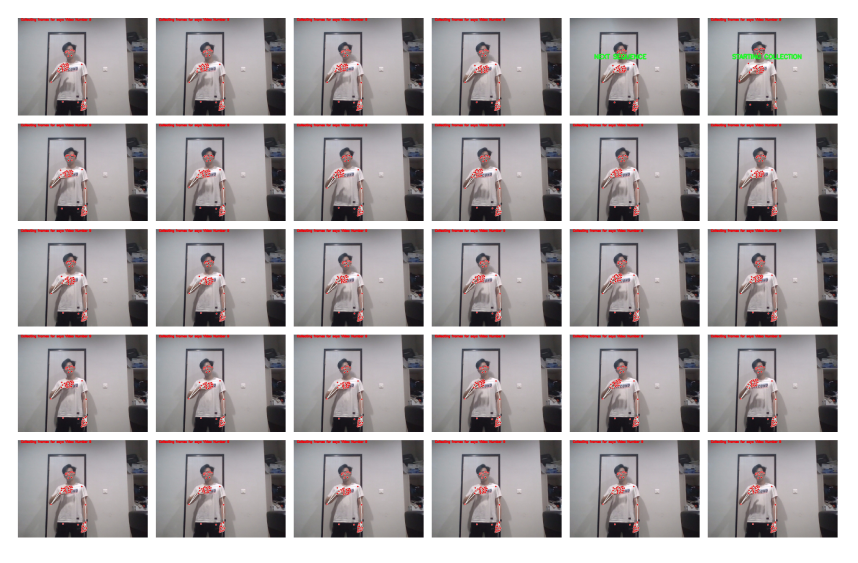
\includegraphics[scale=0.7]{gambar/isyarat-saya.png}

  \caption{Isyarat kosakata 'saya'}
  \label{fig:isyarat-saya}
\end{figure}

\begin{figure}[H]
  \centering

  
\includegraphics[scale=0.7]{gambar/coor-saya.png}

  \caption{Persebaran koordinat 'saya'}
  \label{fig:isyarat-coor-saya}
\end{figure}

\newpage
\section{Pengujian Kondisi Cahaya}
\label{sec:analisiscahaya}

\begin{longtable}{|c|c|}
  \caption{Variasi Kondisi Cahaya}
  \label{tb:kondisicahaya}                                   \\
  \hline
  \rowcolor[HTML]{C0C0C0}
  \textbf{Intensitas Cahaya} & \textbf{Gambar Kondisi}  \\
  \hline
  35 lux            &  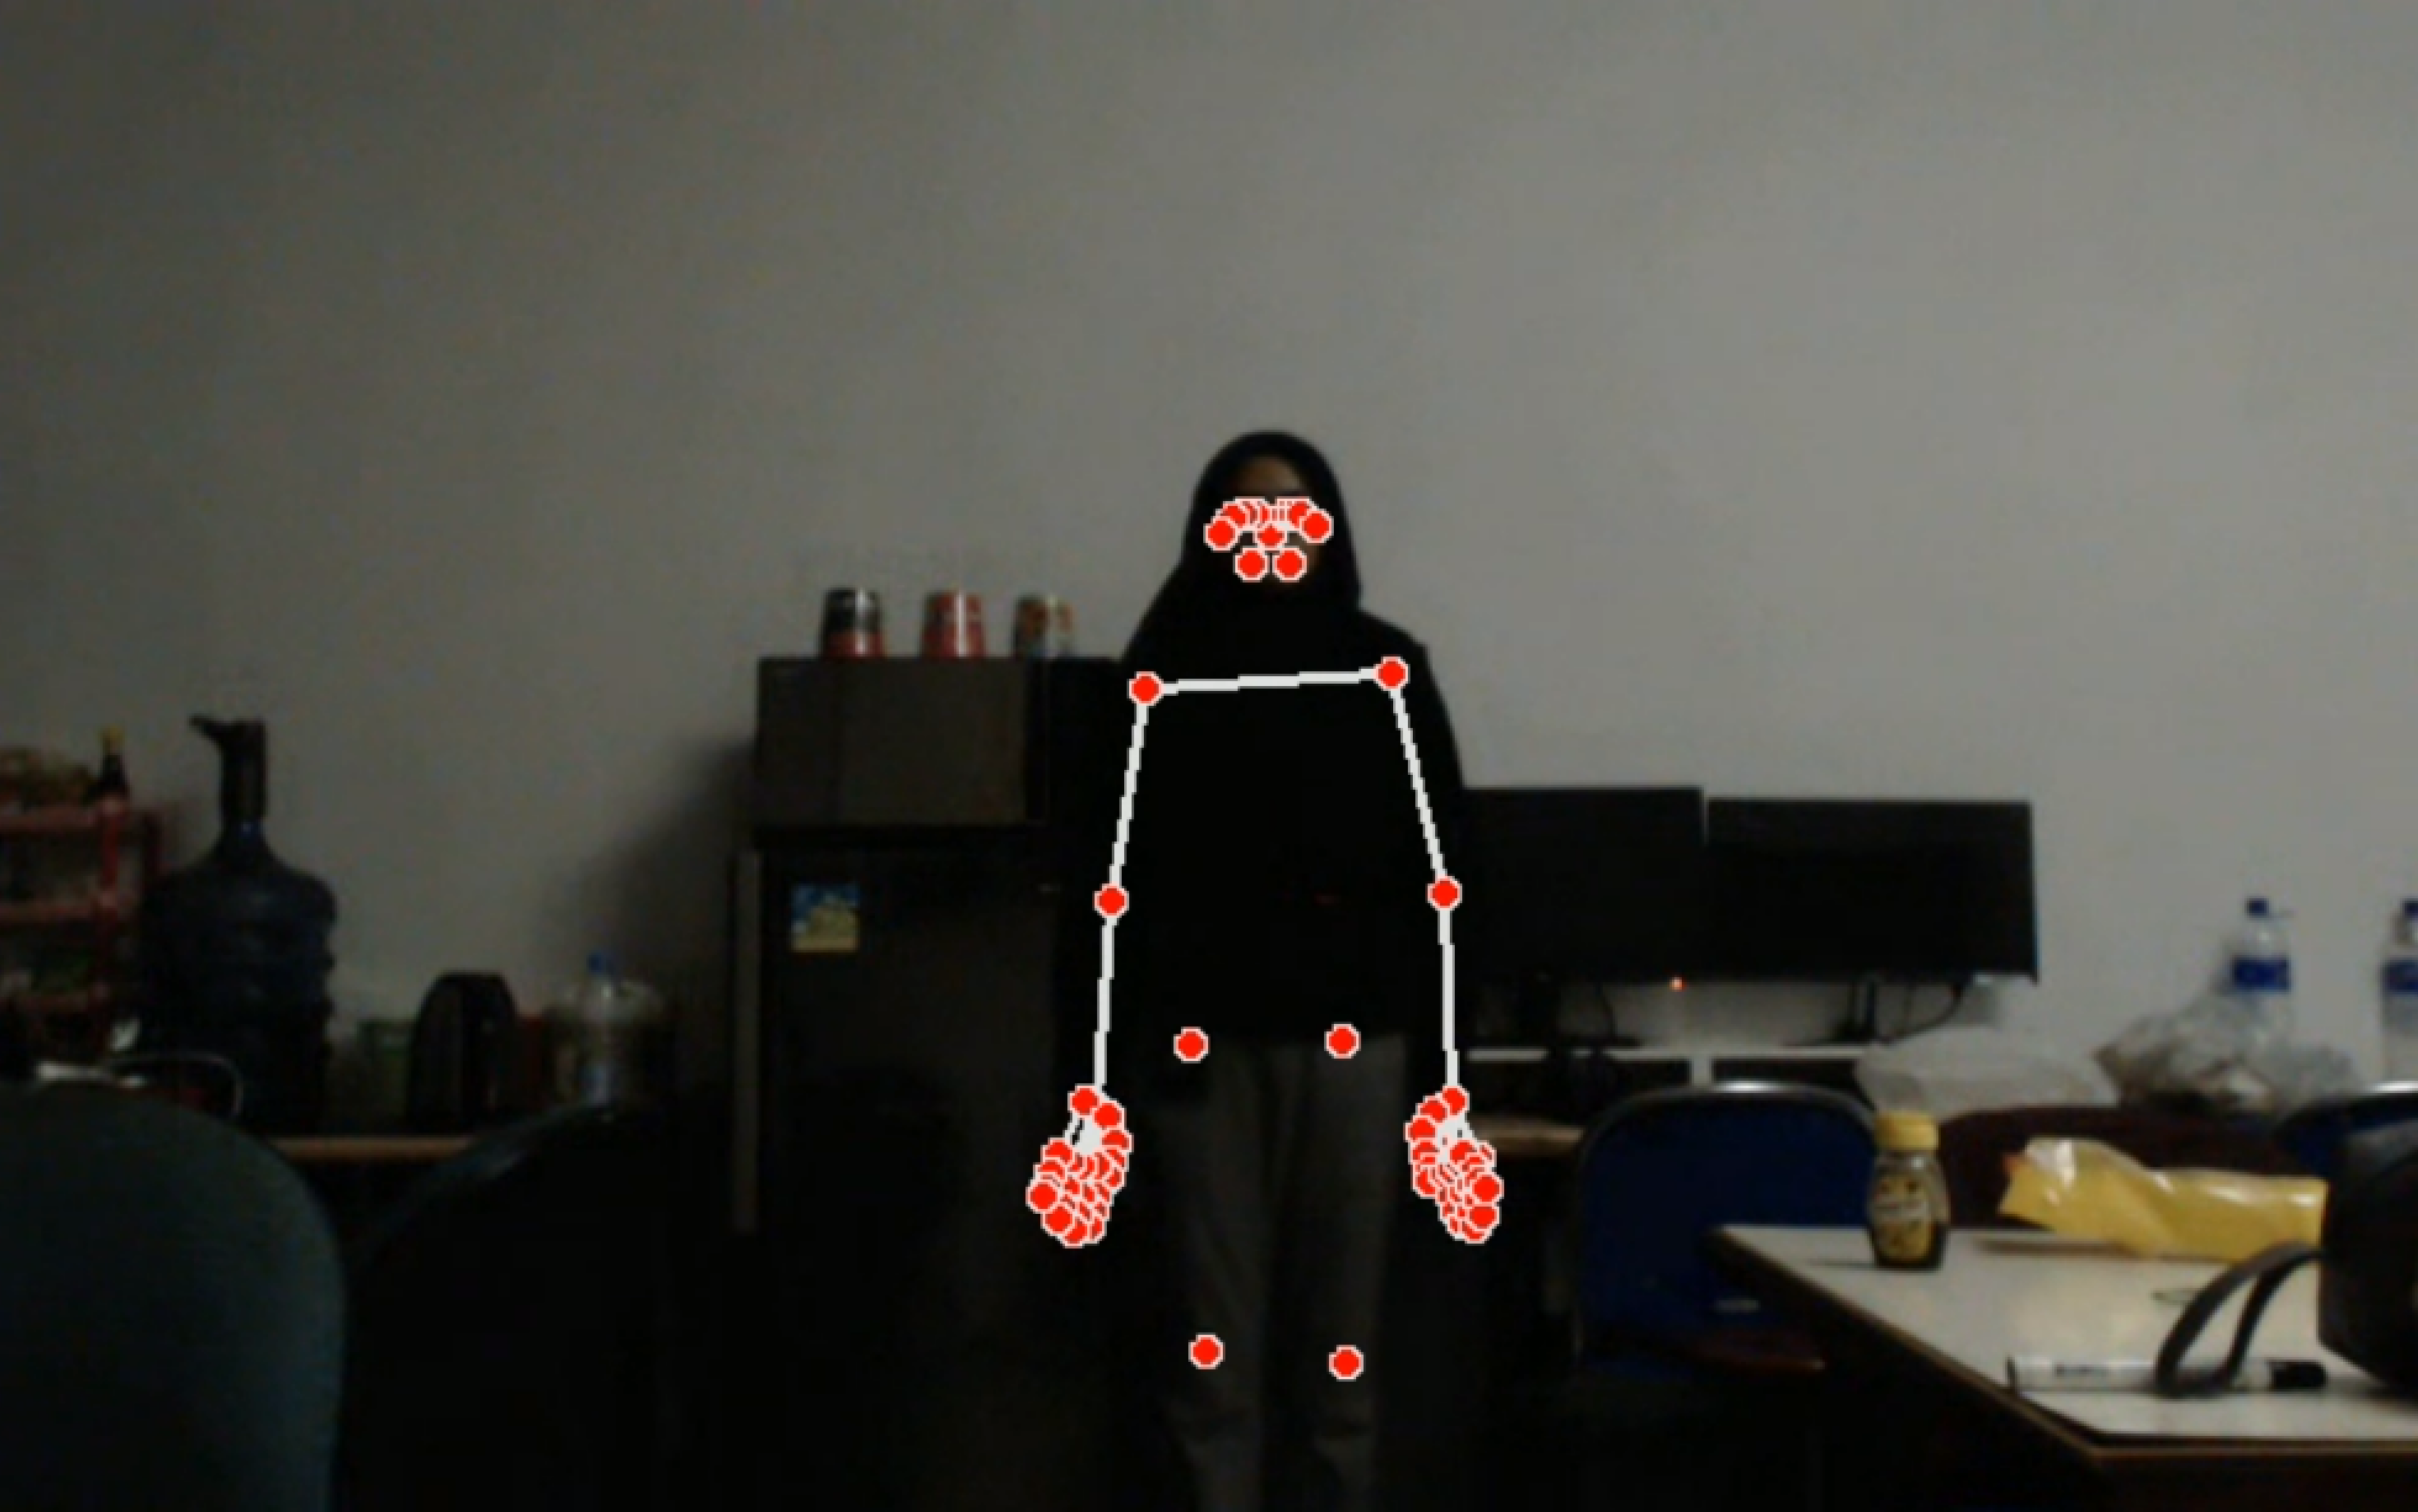
\includegraphics[scale=0.3]{gambar/bab4-gelap.png}                \\
  \hline
  80 lux            & 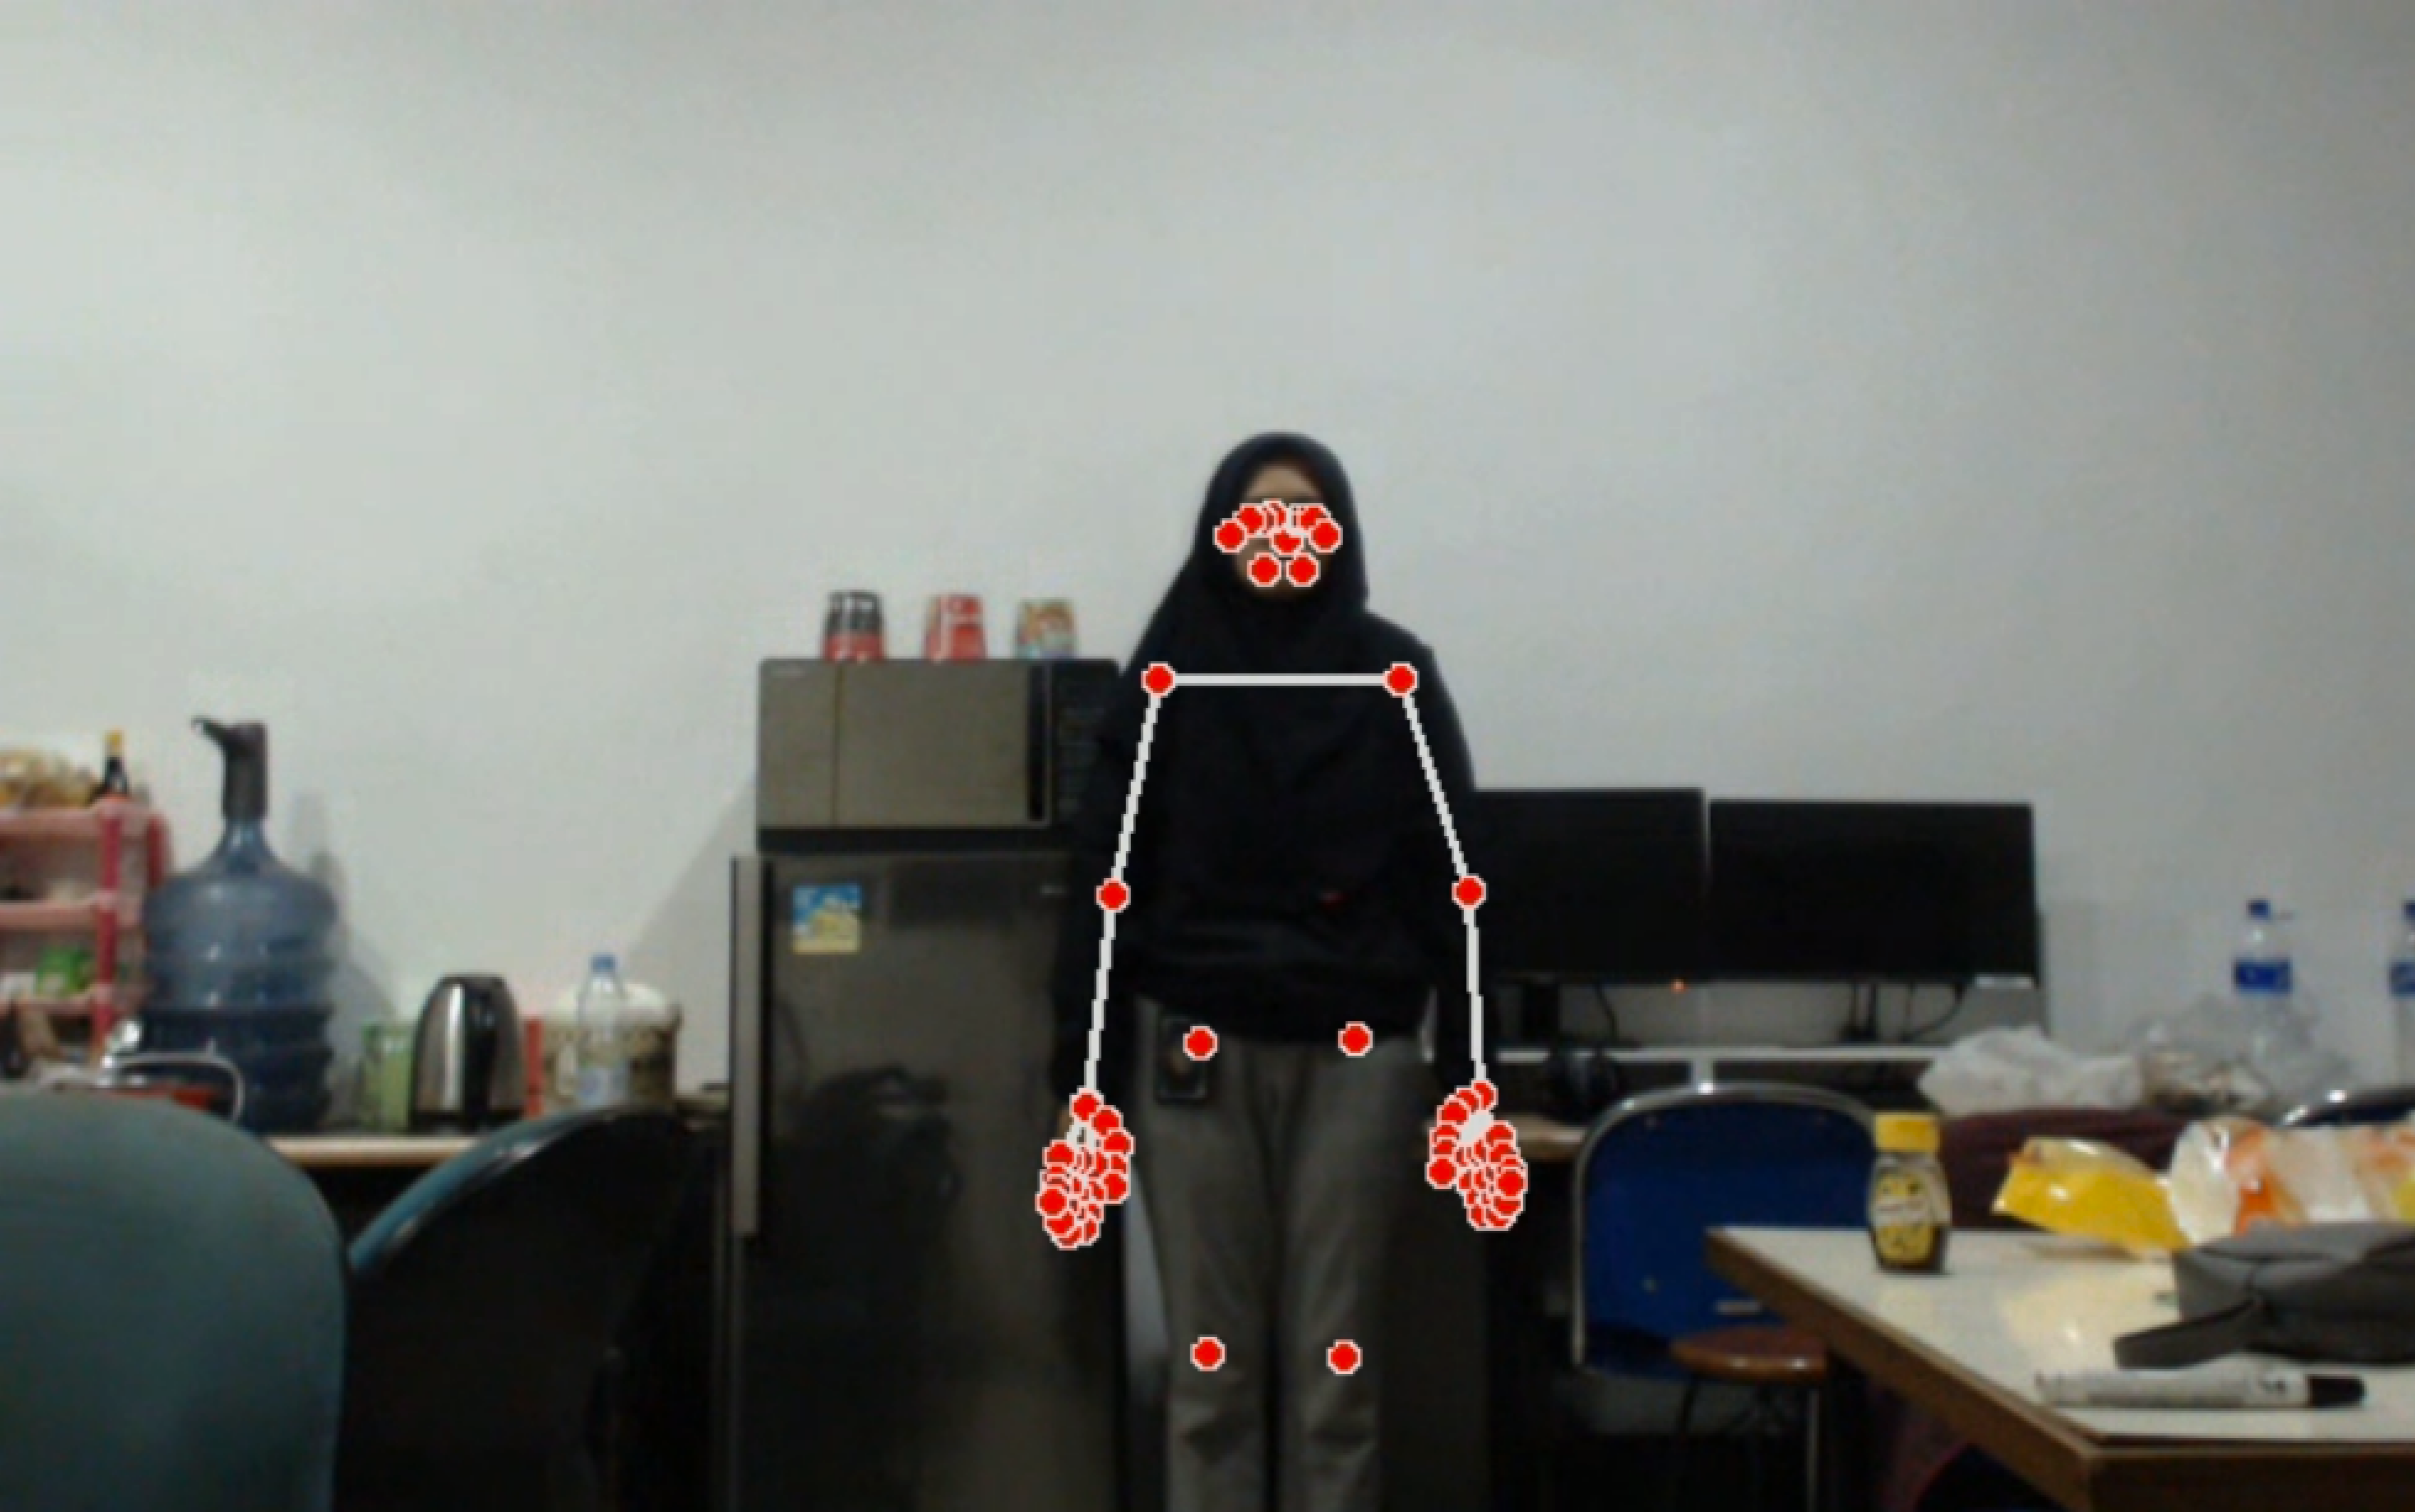
\includegraphics[scale=0.3]{gambar/bab4-remang.png}                 \\
  \hline
  125 lux            & 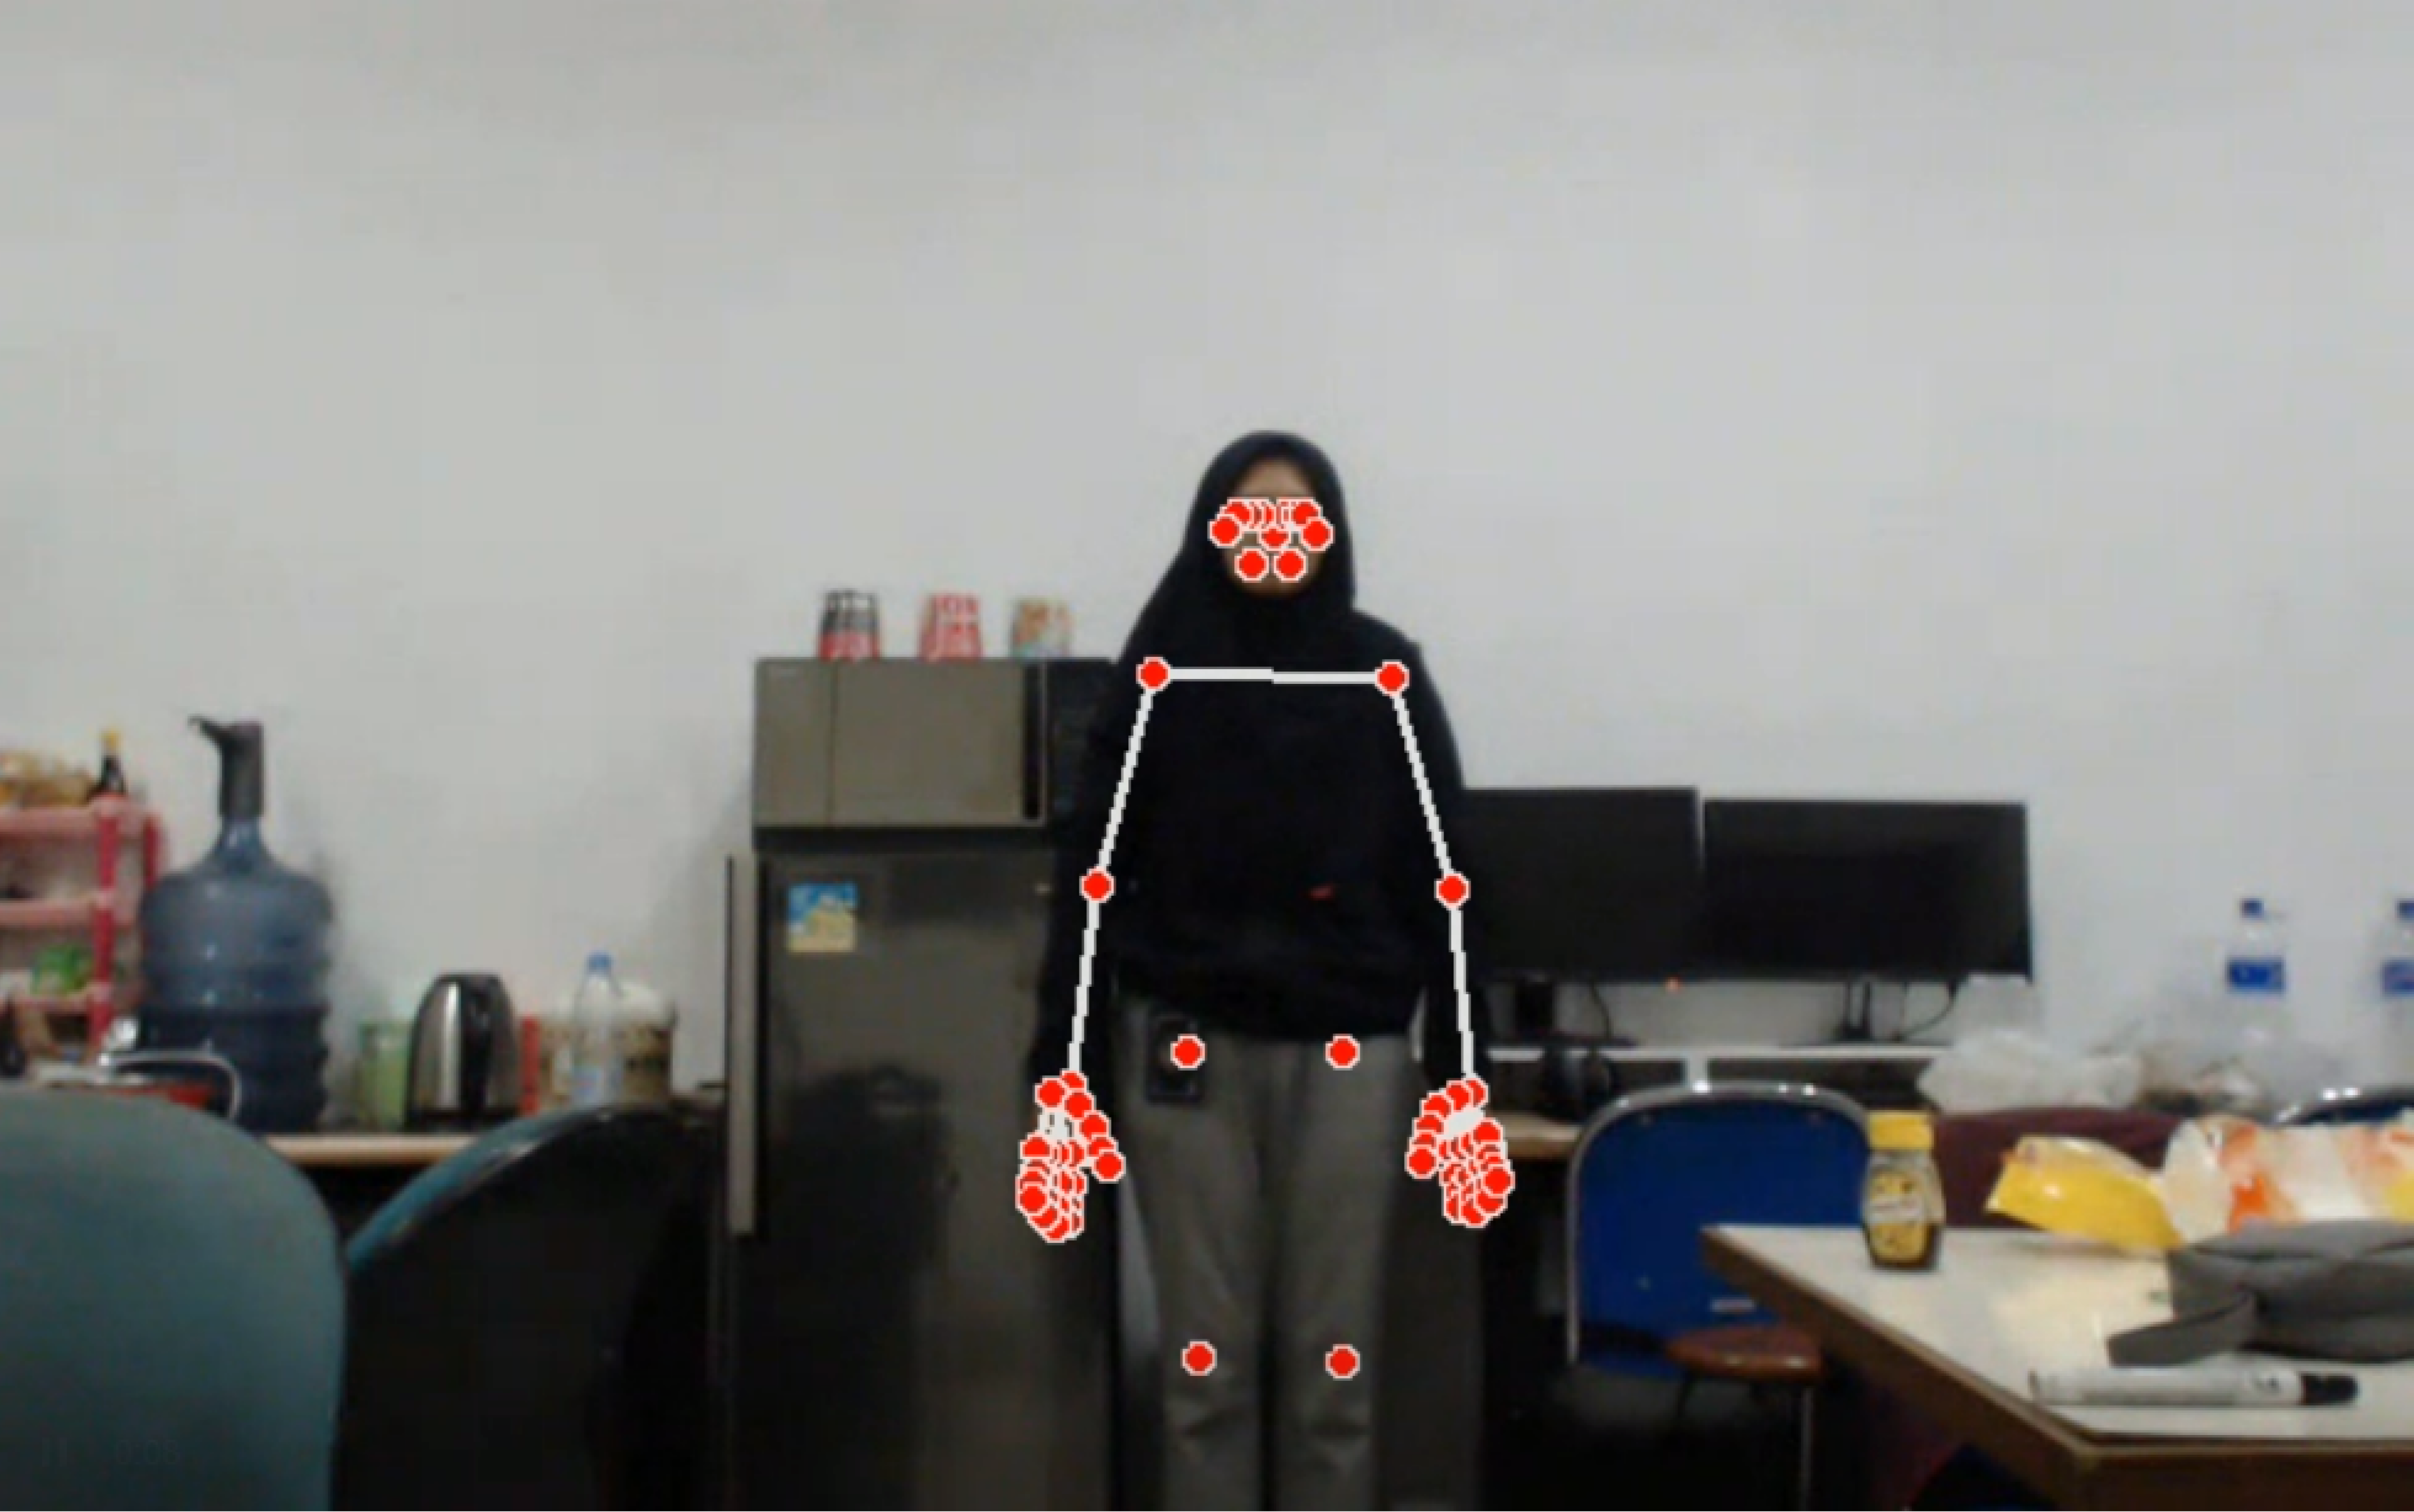
\includegraphics[scale=0.3]{gambar/bab4-terang.png}                 \\
  \hline
\end{longtable}

Pada pengujian kondisi cahaya ini dilakukan untuk memahami bagaimana performa model dalam kondisi intensitas cahaya  yang berbeda - beda. Adapun intensitas cahaya yang akan digunakan pada pengujian ini adalah 35 lux (kondisi ruangan gelap), 80 lux (kondisi ruangan remang - remang), dan 125 lux (kondisi ruangan terang). Variasi intensitas cahaya ini dipilih karena merupakan intensitas cahaya yang umum ditemukan pada ruangan tertutup. Kondisi ruangan dengan intensitas cahaya masing - masing dapat dilihat pada tabel \ref{tb:kondisicahaya}. Pengambilan nilai intensitas cahaya ini dilakukan dengan menggunakan \emph{lux meter} yang telah dikalibrasi untuk memastikan ketelitian hasil pengukuran.

Model penerjemah bahasa Indonesia (BISINDO) yang akan digunakan pada pengujian ini adalah model pada bagian \ref{sec:analisismodel3} karena merupakan model yang menghasilkan klasifikasi yang terbaik jika dibandingkan dengan model lainnya. Untuk setiap intensitas cahaya akan dilakukan pengujian sebanyak tiga kali dengan jarak terhadap kamera sebesar 300 cm. Pada setiap pengujian akan dicari hasil klasifikasi model, waktu yang dibutuhkan model untuk menghasilkan klasifikasi bahasa isyarat berdasarkan data koordinat yang diberikan(\emph{processing time}), waktu total yang dibutuhkan dalam menghasilkan klasifikasi bahasa isyarat (\emph{complete time}), dan rata - rata FPS (\emph{frame per second}) yang didapatkan ketika proses klasifikasi dilakukan pada website.  

\subsection{Pengujian Model di Kondisi Cahaya 35 lux}
\label{sec:analisiscahaya1}

\begin{longtable}{|c|c|c|c|c|}
  \caption{Pengujian Pertama Model di Kondisi Cahaya 35 lux}
  \label{tb:prediksigelap1}                                   \\
  \hline
  \rowcolor[HTML]{C0C0C0}
  \textbf{Kosakata} & \textbf{Klasifikasi Model} & \textbf{\emph{Processing Time}} & \textbf{\emph{Complete Time}} & \textbf{\emph{FPS}}\\
  \hline
  Maaf              & Maaf                          & 0.09209 detik                           & 2.87358 detik                                  & 10.43992871\\
  Tolong            & Tolong                        & 0.09198 detik                           & 2.90961 detik                                  & 10.31065923\\
  Nama              & Nama                          & 0.08932 detik                           & 3.32747 detik                                  & 9.015859368\\
  Saya              & Saya                          & 0.09867 detik                           & 2.88227 detik                                  & 10.40845123\\
  Siapa             & Siapa                         & 0.08973 detik                           & 2.85298 detik                                  & 10.51530802\\
  Rumah             & \textcolor{red}{Delete}       & 0.09612 detik                           & 2.86434 detik                                  & 10.47361061\\
  Delete            & Delete                        & 0.09255 detik                           & 2.82485 detik                                  & 10.62005054\\
  Standby           & Standby                       & 0.09247 detik                           & 2.87624 detik                                  & 10.43027096\\
  Translate         & Translate                     & 0.09525 detik                           & 2.92625 detik                                  & 10.25203914\\
  \hline
\end{longtable}

\begin{longtable}{|c|c|c|c|c|}
  \caption{Pengujian Kedua Model di Kondisi Cahaya 35 lux}
  \label{tb:prediksigelap2}                                   \\
  \hline
  \rowcolor[HTML]{C0C0C0}
  \textbf{Kosakata} & \textbf{Klasifikasi Model} & \textbf{\emph{Processing Time}} & \textbf{\emph{Complete Time}} & \textbf{\emph{FPS}}\\
  \hline
  Maaf              & Maaf                            & 0.10043 detik                           & 3.32854 detik                                   & 9.012933934\\
  Tolong            & Tolong                          & 0.09723 detik                           & 3.31908 detik                                   & 9.038649602\\
  Nama              & \textcolor{red}{Standby}        & 0.08973 detik                           & 2.91430 detik                                   & 10.29405889\\
  Saya              & Saya                            & 0.10072 detik                           & 2.78958 detik                                   & 10.75429474\\
  Siapa             & Siapa                           & 0.08973 detik                           & 3.40174 detik                                   & 8.818992471\\
  Rumah             & Rumah                           & 0.10046 detik                           & 2.94283 detik                                   & 10.19425527\\
  Delete            & Delete                          & 0.09255 detik                           & 2.91633 detik                                   & 10.28691395\\
  Standby           & Standby                         & 0.09182 detik                           & 2.82681 detik                                   & 10.61268775\\
  Translate         & Translate                       & 0.08920 detik                           & 3.39125 detik                                   & 8.846297753\\
  \hline
\end{longtable}


\newpage
\begin{longtable}{|c|c|c|c|c|}
  \caption{Pengujian Ketiga Model di Kondisi Cahaya 35 lux}
  \label{tb:prediksigelap3}                                   \\
  \hline
  \rowcolor[HTML]{C0C0C0}
  \textbf{Kosakata} & \textbf{Klasifikasi Model} & \textbf{\emph{Processing Time}} & \textbf{\emph{Complete Time}} & \textbf{\emph{FPS}}\\
  \hline
  Maaf              & Maaf                          & 0.09209 detik                           & 2.91590 detik                                  & 10.28842795\\
  Tolong            & Tolong                        & 0.09723 detik                           & 3.00149 detik                                  & 9.995029061\\
  Nama              & Nama                          & 0.09725 detik                           & 2.82353 detik                                  & 10.62500063\\
  Saya              & Saya                          & 0.08916 detik                           & 2.96069 detik                                  & 10.13275997\\
  Siapa             & Siapa                         & 0.08973 detik                           & 2.84085 detik                                  & 10.56023606\\
  Rumah             & \textcolor{red}{Delete}       & 0.10066 detik                           & 3.36672 detik                                  & 8.910741828\\
  Delete            & Delete                        & 0.09255 detik                           & 3.43082 detik                                  & 8.744254311\\
  Standby           & Standby                       & 0.09867 detik                           & 3.34507 detik                                  & 8.968416101\\
  Translate         & Translate                     & 0.08920 detik                           & 2.83052 detik                                  & 10.5987426\\
  \hline
\end{longtable}


Berdasarkan tiga pengujian yang telah dilakukan, didapatkan bahwa hampir keseluruhan klasifikasi model yang sesuai dengan \emph{class} kosakata. Namun, terdapat beberapa kesalahan model dalam melakukan klasifikasi. Dapat dilihat pada tabel \ref{tb:prediksigelap1} untuk kosakata "Rumah" diklasifikasikan sebagai "Delete". Kesalahan ini juga terjadi pada tabel \ref{tb:prediksigelap3}. Kemiripan antara gerakan untuk isyarat kosakata "Rumah" dan "Delete", serta kamera yang kesulitan menangkap sepenuhnya pose yang baik menjadi penyebab adanya kesalahan klasifikasi ini. Pada tabel \ref{tb:prediksigelap2}, untuk isyarat kosakata "Nama" diklasifikasikan sebagai "Standby". Kesalahan klasifikasi ini juga disebabkan oleh Mediapipe yang tidak sepenuhnya menangkap pose yang sesuai dengan kosakata "Nama". Pada pengujian ini,  model dapat melakukan klasifikasi yang baik meskipun pengguna berada di dalam kondisi ruangan yang terbilang gelap. Berdasakan data pada tabel \ref{tb:prediksigelap1}, tabel \ref{tb:prediksigelap2}, tabel \ref{tb:prediksigelap3} menunjukkan bahwa secara keseluruhan model memiliki akurasi klasifikasi sebesar 89.9\%. 

Apabila dilihat berdasarkan waktu pemrosesan, rata - rata waktu yang dibutuhkan model untuk menghasilkan klasifikasi bahasa isyarat (\emph{processing time}) adalah 0.093 detik dan rata - rata waktu yang dibutuhkan dalam menghasilkan klasifikasi bahasa isyarat (\emph{complete time}) adalah 3.025 detik. Pada proses pengujian yang dilakukan secara \emph{real time} ini, model memerlukan waktu yang terbilang cepat dalam memproses serangkaian data koordinat yang diberikan. Program penerjemah juga telah mampu menyelesaikan proses klasifikasi dengan cepat. Hal ini menunjukkan bahwa pada kondisi ruangan dengan intensitas cahaya yang cukup gelap, tidak berpengaruh secara signifikan terhadap \emph{processing time} dan \emph{complete time}. Adapun apabila dilihat dari nilai rata - rata FPS yang secara keseluruhan dari 3 pengujian yang dilakukan bernilai 9.968. Nilai ini terbilang cukup baik untuk melakukan klasifikasi gerakan isyarat dengan kondisi ruangan yang terbilang gelap.

Pada pengujian di intensitas cahaya 35 lux, didapat bahwa pengguna tidak dapat melakukan gerakan bahasa isyarat secara cepat. Hal ini disebabkan oleh kondisi ruangan yang gelap ini mempengaruhi kinerja kemampuan kamera dalam menangkap tiap \emph{frame}. Namun, kemampuan \emph{framework} Mediapipe untuk mendeteksi pose pengguna dan melakukan ekstraksi koordinat berdasarkan \emph{landmark} yang ada masih dapat berjalan dengan baik pada kondisi ruangan dengan intensitas cahaya yang kurang baik. Hal ini membantu proses klasifikasi model karena data koordinat yang diproses untuk menghasilkan klasifikasi bahasa isyarat tetap dapat dieksraksi dengan tepat dan tidak memiliki banyak error atau data koordinat kosong (bernilai 0). 

\newpage
\subsection{Pengujian Model di Kondisi Cahaya 80 lux}
\label{sec:analisiscahaya2}

\begin{longtable}{|c|c|c|c|c|}
  \caption{Pengujian Pertama Model di Kondisi Cahaya 80 lux}
  \label{tb:prediksiremang1}                                   \\
  \hline
  \rowcolor[HTML]{C0C0C0}
  \textbf{Kosakata} & \textbf{Klasifikasi Model} & \textbf{\emph{Processing Time}} & \textbf{\emph{Complete Time}} & \textbf{\emph{FPS}}\\
  \hline
  Maaf              & Maaf                         & 0.09171 detik                           & 2.74991 detik                                  & 10.909456\\
  Tolong            & Tolong                       & 0.09063 detik                           & 3.37605 detik                                  & 8.886124329\\
  Nama              & Nama                         & 0.09209 detik                           & 2.93017 detik                                  & 10.23830028\\
  Saya              & Saya                         & 0.09038 detik                           & 2.72305 detik                                  & 11.0170576\\
  Siapa             & Siapa                        & 0.09206 detik                           & 2.84878 detik                                  & 10.53080552\\
  Rumah             & Rumah                        & 0.09353 detik                           & 2.86434 detik                                  & 10.47361061\\
  Delete            & Delete                       & 0.08902 detik                           & 2.87122 detik                                  & 10.44853709\\
  Standby           & Standby                      & 0.08996 detik                           & 3.34507 detik                                  & 8.968416101\\
  Translate         & Translate                    & 0.08869 detik                           & 3.32667 detik                                  & 9.018030454\\
  \hline
\end{longtable}


\begin{longtable}{|c|c|c|c|c|}
  \caption{Pengujian Kedua Model di Kondisi Cahaya 80 lux}
  \label{tb:prediksiremang2}                                   \\
  \hline
  \rowcolor[HTML]{C0C0C0}
  \textbf{Kosakata} & \textbf{Klasifikasi Model} & \textbf{\emph{Processing Time}} & \textbf{\emph{Complete Time}} & \textbf{\emph{FPS}}\\
  \hline
  Maaf              & Maaf                        & 0.09696 detik                           & 3.21279 detik                                 & 9.337690903\\
  Tolong            & Tolong                      & 0.09327 detik                           & 2.82739 detik                                 & 10.61048627\\
  Nama              & Nama                        & 0.09209 detik                           & 2.76493 detik                                 & 10.85019078\\
  Saya              & Saya                        & 0.08996 detik                           & 3.50248 detik                                 & 8.565362827\\
  Siapa             & Siapa                       & 0.08885 detik                           & 2.91064 detik                                 & 10.30701067\\
  Rumah             & Rumah                       & 0.09038 detik                           & 2.89598 detik                                 & 10.35917093\\
  Delete            & Delete                      & 0.09166 detik                           & 2.87689 detik                                 & 10.42791116\\
  Standby           & Standby                     & 0.08996 detik                           & 2.82681 detik                                 & 10.61268775\\
  Translate         & Translate                   & 0.09455 detik                           & 2.88727 detik                                 & 10.39042782\\
  \hline
\end{longtable}



\begin{longtable}{|c|c|c|c|c|}
  \caption{Pengujian Ketiga Model di Kondisi Cahaya 80 lux}
  \label{tb:prediksiremang3}                                   \\
  \hline
  \rowcolor[HTML]{C0C0C0}
  \textbf{Kosakata} & \textbf{Klasifikasi Model} & \textbf{\emph{Processing Time}} & \textbf{\emph{Complete Time}} & \textbf{\emph{FPS}}\\
  \hline
  Maaf              & Maaf                          & 0.08909 detik                           & 2.86751 detik                                  & 10.46203733\\
  Tolong            & Tolong                        & 0.09565 detik                           & 2.89014 detik                                  & 10.38011637\\
  Nama              & Nama                          & 0.09209 detik                           & 3.33049 detik                                  & 9.007688409\\
  Saya              & Saya                          & 0.08996 detik                           & 2.88419 detik                                  & 10.40153358\\
  Siapa             & Siapa                         & 0.08885 detik                           & 2.84085 detik                                  & 10.56023606\\
  Rumah             & \textcolor{red}{Delete}       & 0.08767 detik                           & 3.35699 detik                                  & 8.936581292\\
  Delete            & Delete                        & 0.09129 detik                           & 2.85625 detik                                  & 10.50327421\\
  Standby           & Standby                       & 0.08996 detik                           & 2.87624 detik                                  & 10.43027096\\
  Translate         & Translate                     & 0.09907 detik                           & 2.86400 detik                                  & 10.47486614\\
  \hline
\end{longtable}



Berdasarkan tiga pengujian yang telah dilakukan, didapatkan bahwa hampir keseluruhan klasifikasi model telah sesuai dengan \emph{class} kosakatanya. Hal ini menunjukkan bahwa peningkatan intensitas cahaya berpengaruh dalam proses klasifikasi yang dilakukan oleh model. Adanya peningkatan intensitas cahaya atau semakin terang kondisi ruangan menghasilkan klasifikasi model yang lebih baik dan tepat sesuai dengan kosakata yang selaras dengan gerakannya. Namun, masih terdapat kesalahan model dalam melakukan klasifikasi. Dapat dilihat pada tabel \ref{tb:prediksiremang3}, untuk isyarat kosakata "Rumah" diklasifikasikan sebagai "Delete". Hal ini disebabkan karena adanya kemiripan antara gerakan untuk kosakata "Rumah" dan "Delete" sehingga apabila pengguna melakukan gerakan isyarat dengan tidak mengutamakan keunikan atau \emph{feature}, dapat menghasilkan klasifikasi yang salah. Berdasarkan tabel \ref{tb:prediksiremang1}, tabel \ref{tb:prediksiremang2}, dan tabel tabel \ref{tb:prediksiremang3} menunjukkan bahwa secara keseluruhan model memiliki akurasi klasifikasi sebesar 96.2\%.

Apabila dilihat berdasarkan waktu pemrosesan, rata - rata waktu yang dibutuhkan model untuk menghasilkan klasifikasi bahasa isyarat (\emph{processing time}) adalah 0.091 detik dan rata - rata waktu yang dibutuhkan dalam menghasilkan klasifikasi bahasa isyarat (\emph{complete time}) adalah 2.982  detik. Dapat dilihat bahwa terdapat peningkatan \emph{processing time} dan \emph{complete time} seiring dengan peningkatan intensitas cahaya ruangan, dimana kemampuan kamera dalam menangkap gerakan bahasa isyarat lebih mudah dan jelas lagi. Hal ini juga berkaitan dengan kemampuan program dalam mengekstrak koordinat yang dibutuhkan untuk menghasilkan klasifikasi, serta lama waktu yang dibutuhkan kamera dalam menangkap tiap \emph{frame} yang nantinya digunakan untuk mendapatkan data koordinat menjadi lebih cepat. Adapun nilai rata - rata FPS yang didapatkan berdasarkan 3 pengujian yang dilakukan bernilai 10.115. Apabila dilihat dari pengujian sebelumnya, didapatkan bahwa terdapat peningkatan antara rata - rata nilai FPS seiring dengan peningkatan intensitas cahaya ruangan.

\subsection{Pengujian Model di Kondisi Cahaya 125 lux}
\label{sec:analisiscahaya3}

\begin{longtable}{|c|c|c|c|c|}
  \caption{Pengujian Pertama Model di Kondisi Cahaya 125 lux}
  \label{tb:prediksiterang1}                                   \\
  \hline
  \rowcolor[HTML]{C0C0C0}
  \textbf{Kosakata} & \textbf{Klasifikasi Model} & \textbf{\emph{Processing Time}} & \textbf{\emph{Complete Time}} & \textbf{\emph{FPS}}\\
  \hline
  Maaf              & Maaf                        & 0.09605 detik                           & 2.82092 detik                                 & 10.63483378\\
  Tolong            & Tolong                      & 0.09398 detik                           & 1.42116 detik                                 & 21.10957663\\
  Nama              & Nama                        & 0.09418 detik                           & 2.78056 detik                                 & 10.78920643\\
  Saya              & Saya                        & 0.09123 detik                           & 2.76447 detik                                 & 10.85198745\\
  Siapa             & Siapa                       & 0.09382 detik                           & 2.78827 detik                                 & 10.7593708\\
  Rumah             & Rumah                       & 0.09245 detik                           & 3.08035 detik                                 & 9.73915628\\
  Delete            & Delete                      & 0.08884 detik                           & 2.84831 detik                                 & 10.53255086\\
  Standby           & Standby                     & 0.09215 detik                           & 1.42673 detik                                 & 21.02713678\\
  Translate         & Translate                   & 0.09544 detik                           & 2.93033 detik                                 & 10.23775049\\
  \hline
\end{longtable}


\begin{longtable}{|c|c|c|c|c|}
  \caption{Pengujian Kedua Model di Kondisi Cahaya 125 lux}
  \label{tb:prediksiterang2}                                   \\
  \hline
  \rowcolor[HTML]{C0C0C0}
  \textbf{Kosakata} & \textbf{Klasifikasi Model} & \textbf{\emph{Processing Time}} & \textbf{\emph{Complete Time}} & \textbf{\emph{FPS}}\\
  \hline
  Maaf              & Maaf                        & 0.09328 detik                           & 2.73007 detik                                 & 10.98871341\\
  Tolong            & Tolong                      & 0.08798 detik                           & 1.45114 detik                                 & 20.67340944\\
  Nama              & Nama                        & 0.09166 detik                           & 2.74389 detik                                 & 10.93340076\\
  Saya              & Saya                        & 0.09123 detik                           & 2.84037 detik                                 & 10.56201777\\
  Siapa             & Siapa                       & 0.09120 detik                           & 2.91372 detik                                 & 10.29610573\\
  Rumah             & Rumah                       & 0.09164 detik                           & 2.82356 detik                                 & 10.62489297\\
  Delete            & Delete                      & 0.09363 detik                           & 2.67091 detik                                 & 11.2321354\\
  Standby           & Standby                     & 0.09108 detik                           & 1.39669 detik                                 & 21.47940042\\
  Translate         & Translate                   & 0.10021 detik                           & 3.09649 detik                                 & 9.688404324\\
  \hline
\end{longtable}


\begin{longtable}{|c|c|c|c|c|}
  \caption{Pengujian Ketiga Model di Kondisi Cahaya 125 lux}
  \label{tb:prediksiterang3}                                   \\
  \hline
  \rowcolor[HTML]{C0C0C0}
  \textbf{Kosakata} & \textbf{Klasifikasi Model} & \textbf{\emph{Processing Time}} & \textbf{\emph{Complete Time}} & \textbf{\emph{FPS}}\\
  \hline
  Maaf              & Maaf                        & 0.09278 detik                           & 2.82092 detik                                 & 10.63483378\\
  Tolong            & Tolong                      & 0.09278 detik                           & 1.46072 detik                                 & 20.53786302\\
  Nama              & Nama                        & 0.09398 detik                           & 2.82560 detik                                 & 10.61722782\\
  Saya              & Saya                        & 0.09706 detik                           & 2.85545 detik                                 & 10.50622087\\
  Siapa             & Siapa                       & 0.08928 detik                           & 2.67342 detik                                 & 11.22158755\\
  Rumah             & Rumah                       & 0.09007 detik                           & 2.76350 detik                                 & 10.85577924\\
  Delete            & Delete                      & 0.09212 detik                           & 2.73070 detik                                 & 10.9862093\\
  Standby           & Standby                     & 0.09168 detik                           & 1.45698 detik                                 & 20.59049293\\
  Translate         & Translate                   & 0.09213 detik                           & 2.90930 detik                                 & 10.31174923\\
  \hline
\end{longtable}



Berdasarkan tiga pengujian yang telah dilakukan, didapat bahwa keseluruhan klasifikasi model telah sesuai dengan \emph{class} kosakatanya. Hal ini menunjukkan bahwa semakin terang atau peningkatan intensitas cahaya berpengaruh dalam proses klasifikasi yang dilakukan oleh model. Pada tingkat intensitas cahaya tertinggi pada pengujian ini, dihasilkan klasifikasi yang baik dan tepat untuk seluruh kosakatanya. Berdasarkan data pada tabel \ref{tb:prediksiterang1}, tabel \ref{tb:prediksiterang2}, tabel \ref{tb:prediksiterang3} menunjukkan bahwa model memiliki akurasi klasifikasi sebesar 100\%.

Apabila dilihat berdasarkan waktu pemrosesan, rata - rata waktu yang dibutuhkan model untuk menghasilkan klasifikasi bahasa isyarat (\emph{processing time}) adalah 0.093 detik dan rata - rata waktu yang dibutuhkan dalam menghasilkan klasifikasi bahasa isyarat (\emph{complete time}) adalah 2.519 detik. Dapat dilihat bahwa terdapat peningkatan \emph{complete time} seiring dengan meningkatnya intensitas cahaya ruangan. Hal ini menunjukkan bahwa kemampuan kamera dalam menangkap gerakan bahasa isyarat lebih mudah dan jelas lagi sehingga dalam memproses tiap \emph{frame} yang nantinya digunakan untuk mendapatkan data koordinat menjadi lebih cepat. Namun, kenaikan intensitas cahaya tidak menyebabkan kenaikan terhadap \emph{processing time}. Apabila dibandingkan dengan pengujian pada intensitas cahaya 80 lux, terdapat penurunan sebesar 0.002 detik. Penurunan ini terbilang sangat kecil dan tidak mempengaruhi pengalaman pengguna dalam menggunakan program penerjemah bahasa isyarat Indonesia (BISINDO) secara keseluruhan. Adanya penurunan \emph{processing time} dapat disebabkan oleh ekstraksi koordinat pada tiap \emph{frame} yang lebih baik lagi, dimana untuk 108 koordinat yang digunakan memiliki suatu nilai dan tidak bernilai 0 (pada \emph{framework} Mediapipe apabila suatu koordinat tidak terdeteksi, maka akan otomatis bernilai 0). Hal ini berdampak pada model yang harus memproses lebih banyak lagi untuk menghasilkan klasifikasi bahasa isyarat. Adapun nilai rata - rata FPS yang didapatkan berdasarkan 3 pengujian yang dilakukan bernilai 12.905. Apabila dilihat dari 2 pengujian sebelumnya, didapatkan bahwa terdapat peningkatan antara rata - rata nilai FPS seiring dengan peningkatan intensitas cahaya ruangan. Peningkatan nilai ini juga menunjukkan bahwa addanya hubungan antara kenaikan intensitas cahaya yang memberikan kemudahan bagi kamera dalam menangkap citra yang lebih jelas dan detail lagi sehingga sistem menghasilkan performa yang lebih baik dan menghasilkan klasifikasi yang lebih akurat lagi.

\newpage
\subsection{Rangkuman Pengujian Kondisi Cahaya}
\label{sec:analisisrangkumancahaya}

\begin{longtable}{|c|c|c|c|c|}
  \caption{Rangkuman Pengujian Kondisi Cahaya}
  \label{tb:evaluasiCahaya}                                   \\
  \hline
  \rowcolor[HTML]{C0C0C0}
  \textbf{Cahaya} & \textbf{Akurasi} & \emph{\textbf{Avg. Processing Time}} & \emph{\textbf{Avg. Complete Time}} &\textbf{FPS} \\
  \hline
  35 lux & 0.89 & 0.0938 detik & 3.0335 detik  & 9.968\\
  80 lux & 0.96 & 0.0918 detik & 2.9928 detik  & 10.115\\
  125 lux & 1.00 & 0.0923 detik & 2.4777 detik & 12.905\\
  \hline
\end{longtable}

Secara keseluruhan, dapat dilihat bahwa model dapat beradaptasi dengan baik terhadap perubahan intensitas cahaya. Pada tabel \ref{tb:evaluasiCahaya} dapat dilihat dengan nilai akurasi yang masih berada diatas 0.85 atau 85\%. Nilai akurasi cenderung meningkat seiring dengan semakin meningkatnya intensitas cahaya pada suatu ruangan. Akurasi tertinggi, yaitu pada nilai intensitas cahaya 125 lux oleh kenaikan intensitas cahaya yang memudahkan kamera dalam menangkap gerakan isyarat pengguna dengan lebih jelas dan detail lagi sehingga nantinya \emph{framework} MediaPipe dapat mendapatkan data koordinat dengan lebih akurat lagi. Adapun pada nilai \emph{average complete time} terdapat penurunan yang cukup signifikan seiring dengan peningkatan intensitas cahaya. Penurunan juga terjadi pada nilai \emph{average processing time}. Seiring dengan peningkatan intensitas cahaya juga berpengaruh dengan peningkatan nilai rata - rata FPS. Adapun dapat dilihat bahwa adanya hubungan antara kenaikan intensitas cahaya yang memberikan kemudahan bagi kamera dalam menangkap citra yang lebih jelas dan detail lagi sehingga sistem menghasilkan performa yang lebih baik dan menghasilkan klasifikasi yang lebih akurat lagi.

\section{Pengujian Kondisi Jarak}
\label{sec:analisisjarak}

Pada pengujian kondisi jarak ini dilakukan untuk memahami bagaimana performa model pada jarak kamera dengan pengguna yang berbeda - beda. Adapun jarak yang akan digunakan pada pengujian ini adalah 180 cm, 240 cm, dan 300 cm. Variasi jarak ini dipilih dengan mempertimbangkan bahwa bagian kepala hingga tangan pengguna dapat terlihat secara jelas pada kamera sehingga setiap gerakan bahasa isyarat yang akan dilakukan. Untuk menghasilkan klasifikasi model diperlukan 30 \emph{frame} dan untuk setiap \emph{frame} diekstraksi koordinatnya dengan menggunakan \emph{framework} Mediapipe, apabila bagian tubuh pengguna (terkhususnya tangan dan kepala yang dominan digunakan untuk merepresentasikan suatu bahasa isyarat) tidak terlihat pada kamera akan mempengaruhi data koordinat yang didapatkan dan menyulitkan model untuk melakukan klasifikasi dengan tepat. Adapun posisi pengguna dengan jarak masing - masing dapat dlihat pada tabel \ref{tb:kondisijarak}. 

Model penerjemah bahasa Indonesia (BISINDO) yang akan digunakan pada pengujian ini adalah model pada bagian \ref{sec:analisismodel3} karena merupakan model yang menghasilkan klasifikasi yang terbaik jika dibandingkan dengan model lainnya. Untuk setiap variasi jarak akan dilakukan pengujian sebanyak tiga kali dengan kondisi ruangan yang memiliki intensitas cahaya yang terang (berkisar pada 125 lux). Pada setiap pengujian akan dicari hasil klasifikasi model, waktu yang dibutuhkan model untuk menghasilkan klasifikasi bahasa isyarat berdasarkan data koordinat yang diberikan(\emph{processing time}), waktu total yang dibutuhkan dalam menghasilkan klasifikasi bahasa isyarat (\emph{complete time}), dan rata - rata FPS (\emph{frame per second}) yang didapatkan ketika proses klasifikasi dilakukan pada website. 

\newpage
\begin{longtable}{|c|c|}
  \caption{Variasi Kondisi Jarak}
  \label{tb:kondisijarak}                                   \\
  \hline
  \rowcolor[HTML]{C0C0C0}
  \textbf{Jarak} & \textbf{Gambar Kondisi}  \\
  \hline
  180 cm            &  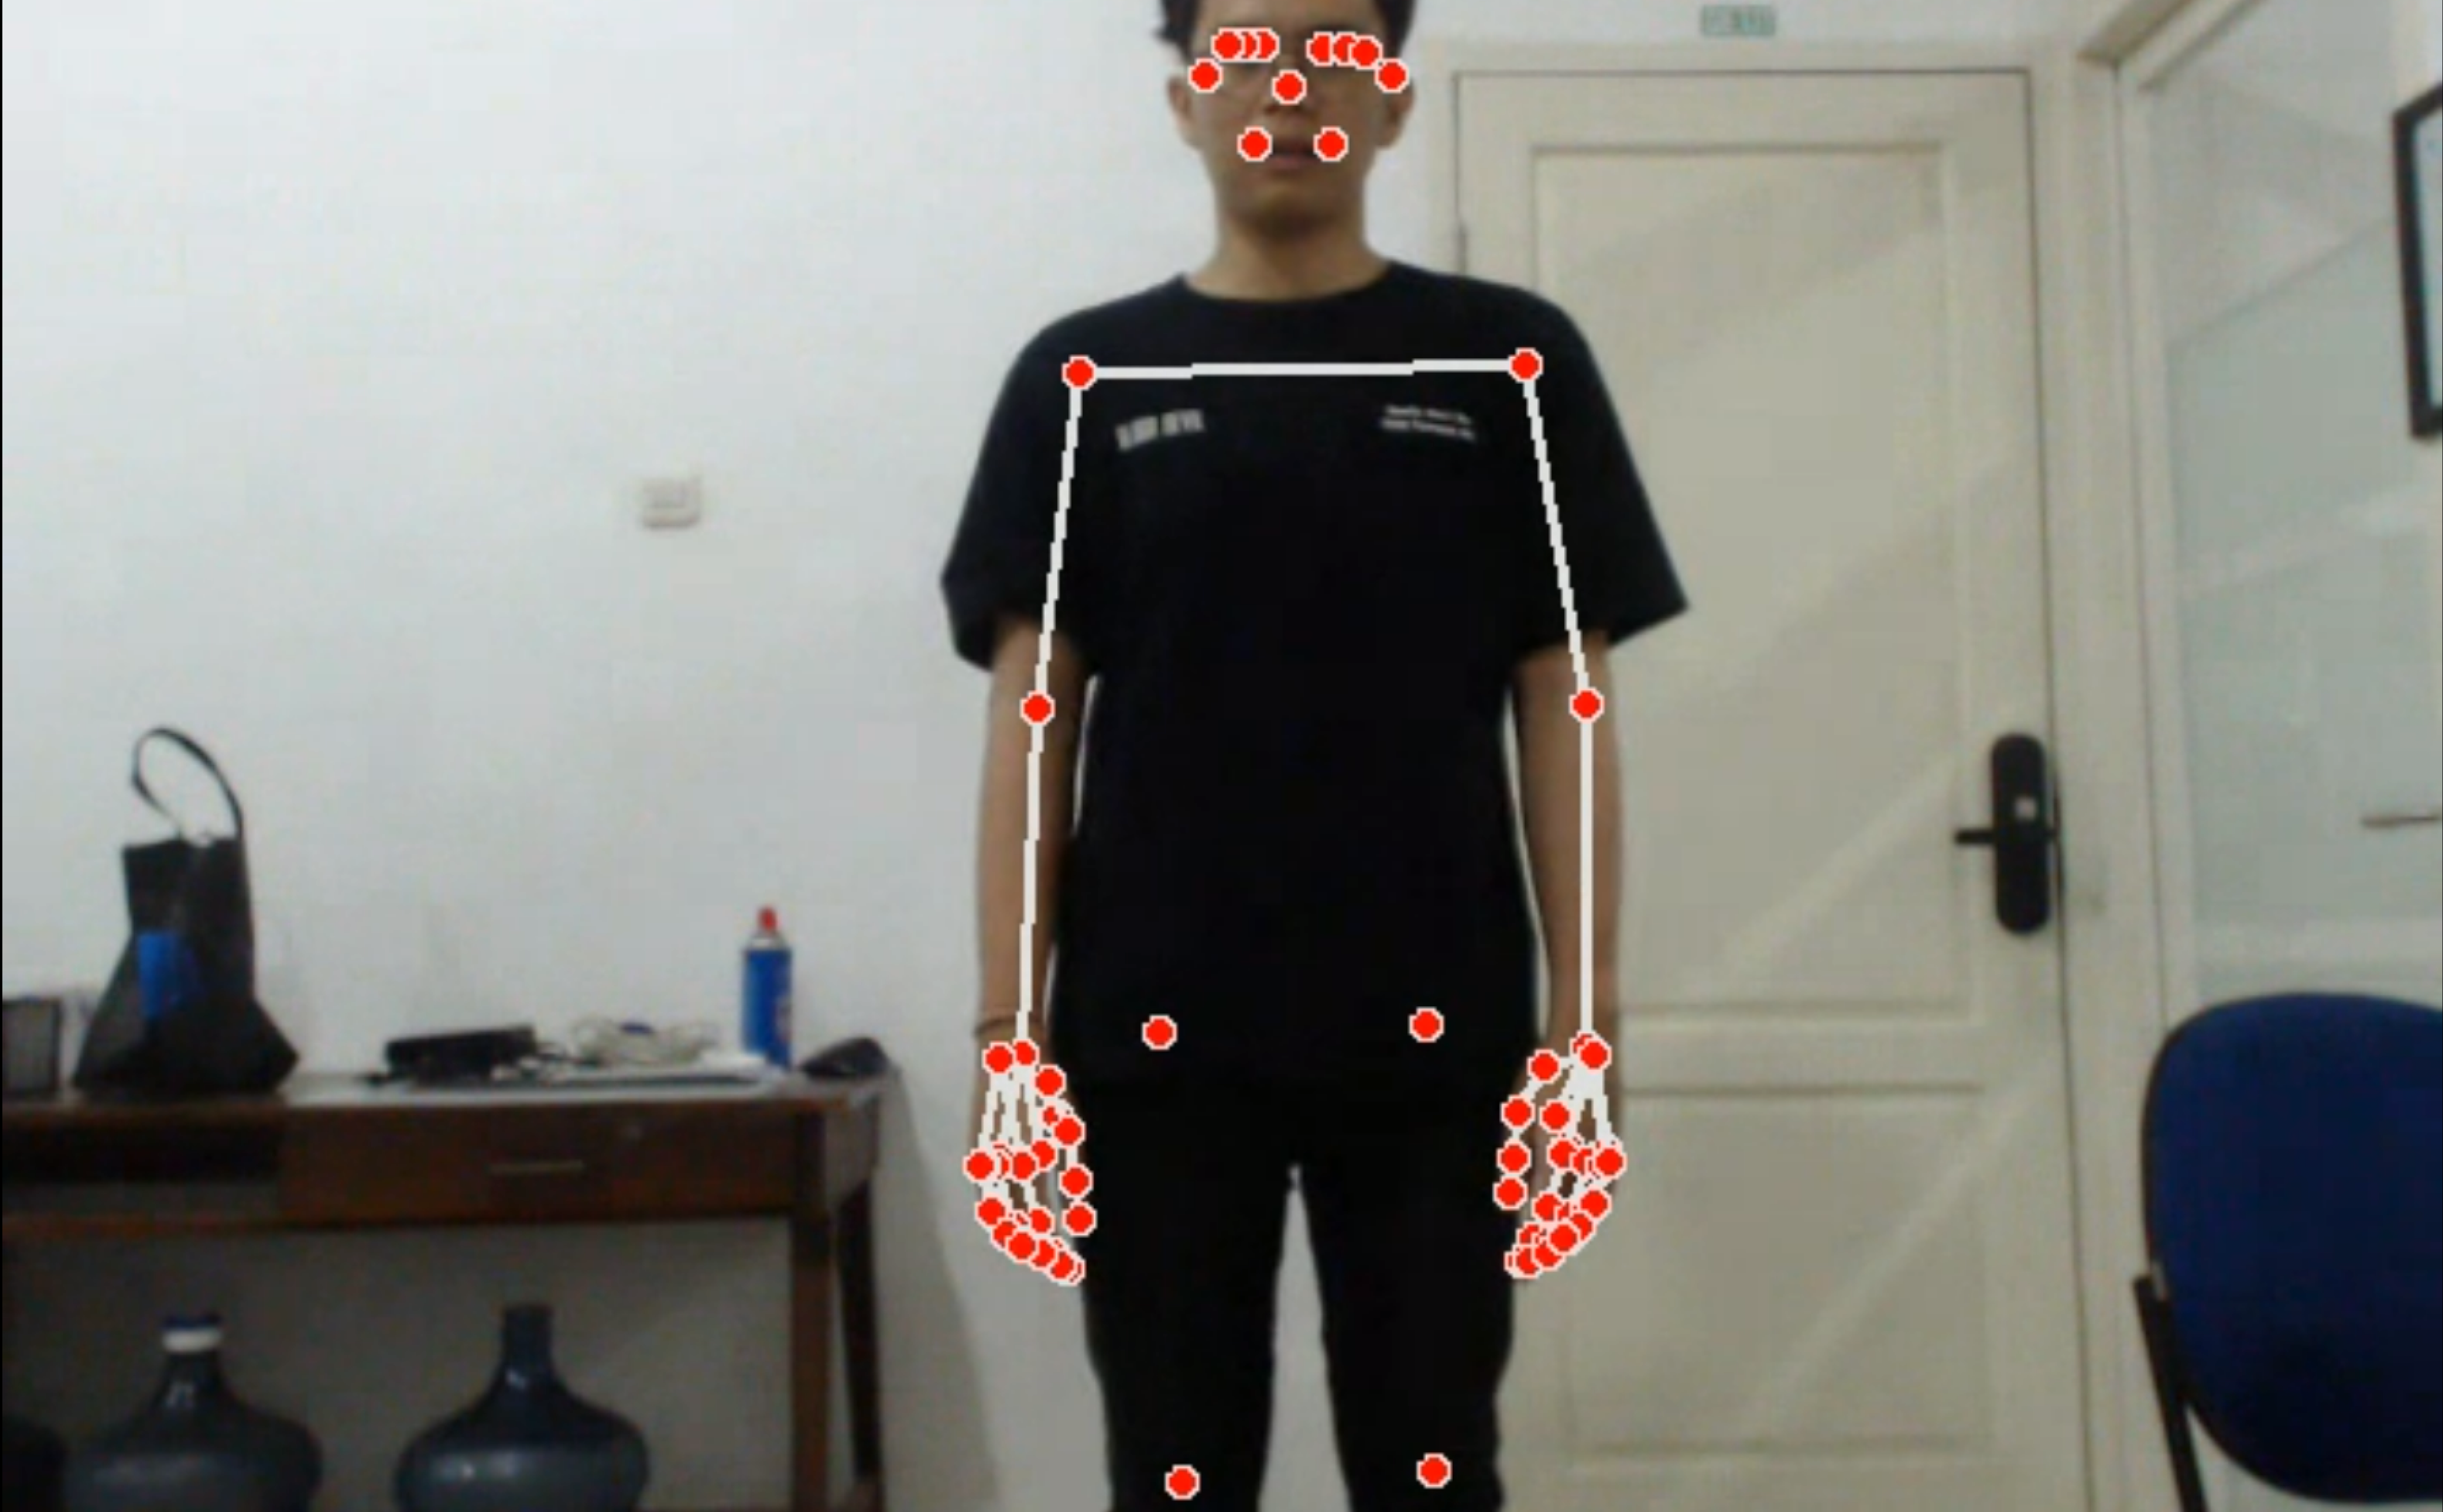
\includegraphics[scale=0.17]{gambar/bab4-jarak300.png}                \\
  \hline
  240 cm            & 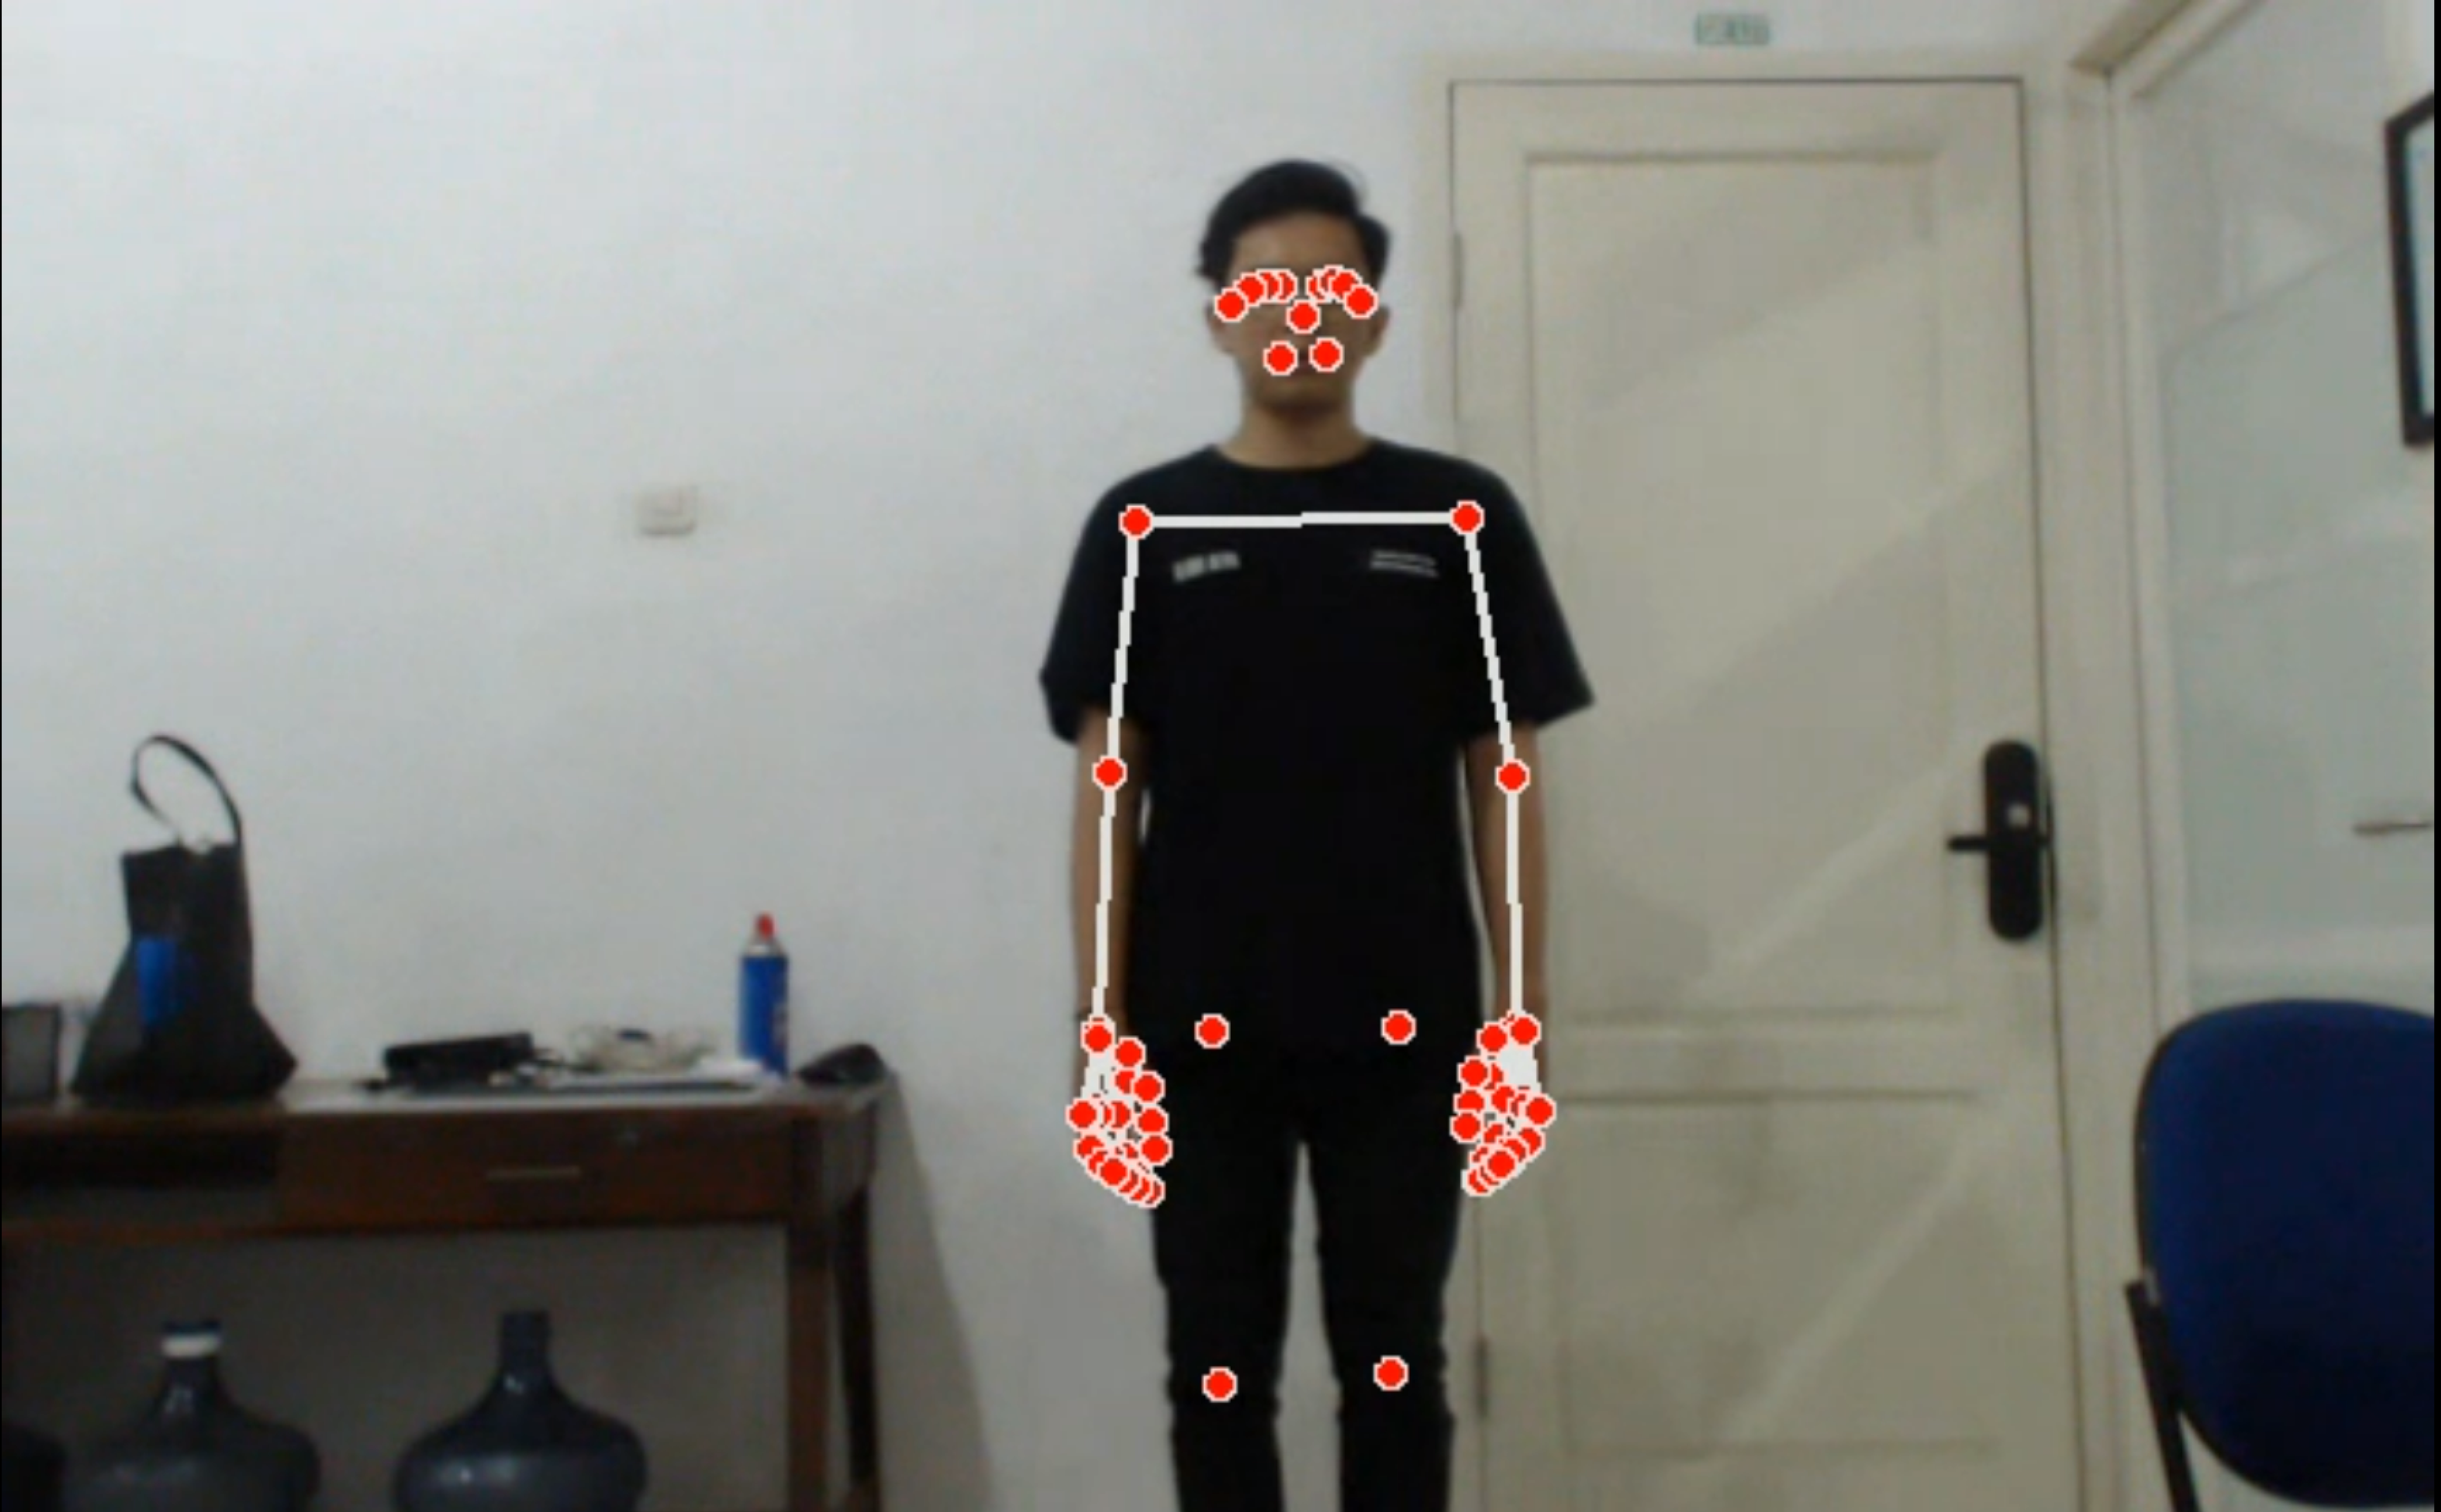
\includegraphics[scale=0.17]{gambar/bab4-jarak240.png}                 \\
  \hline
  300 cm            & 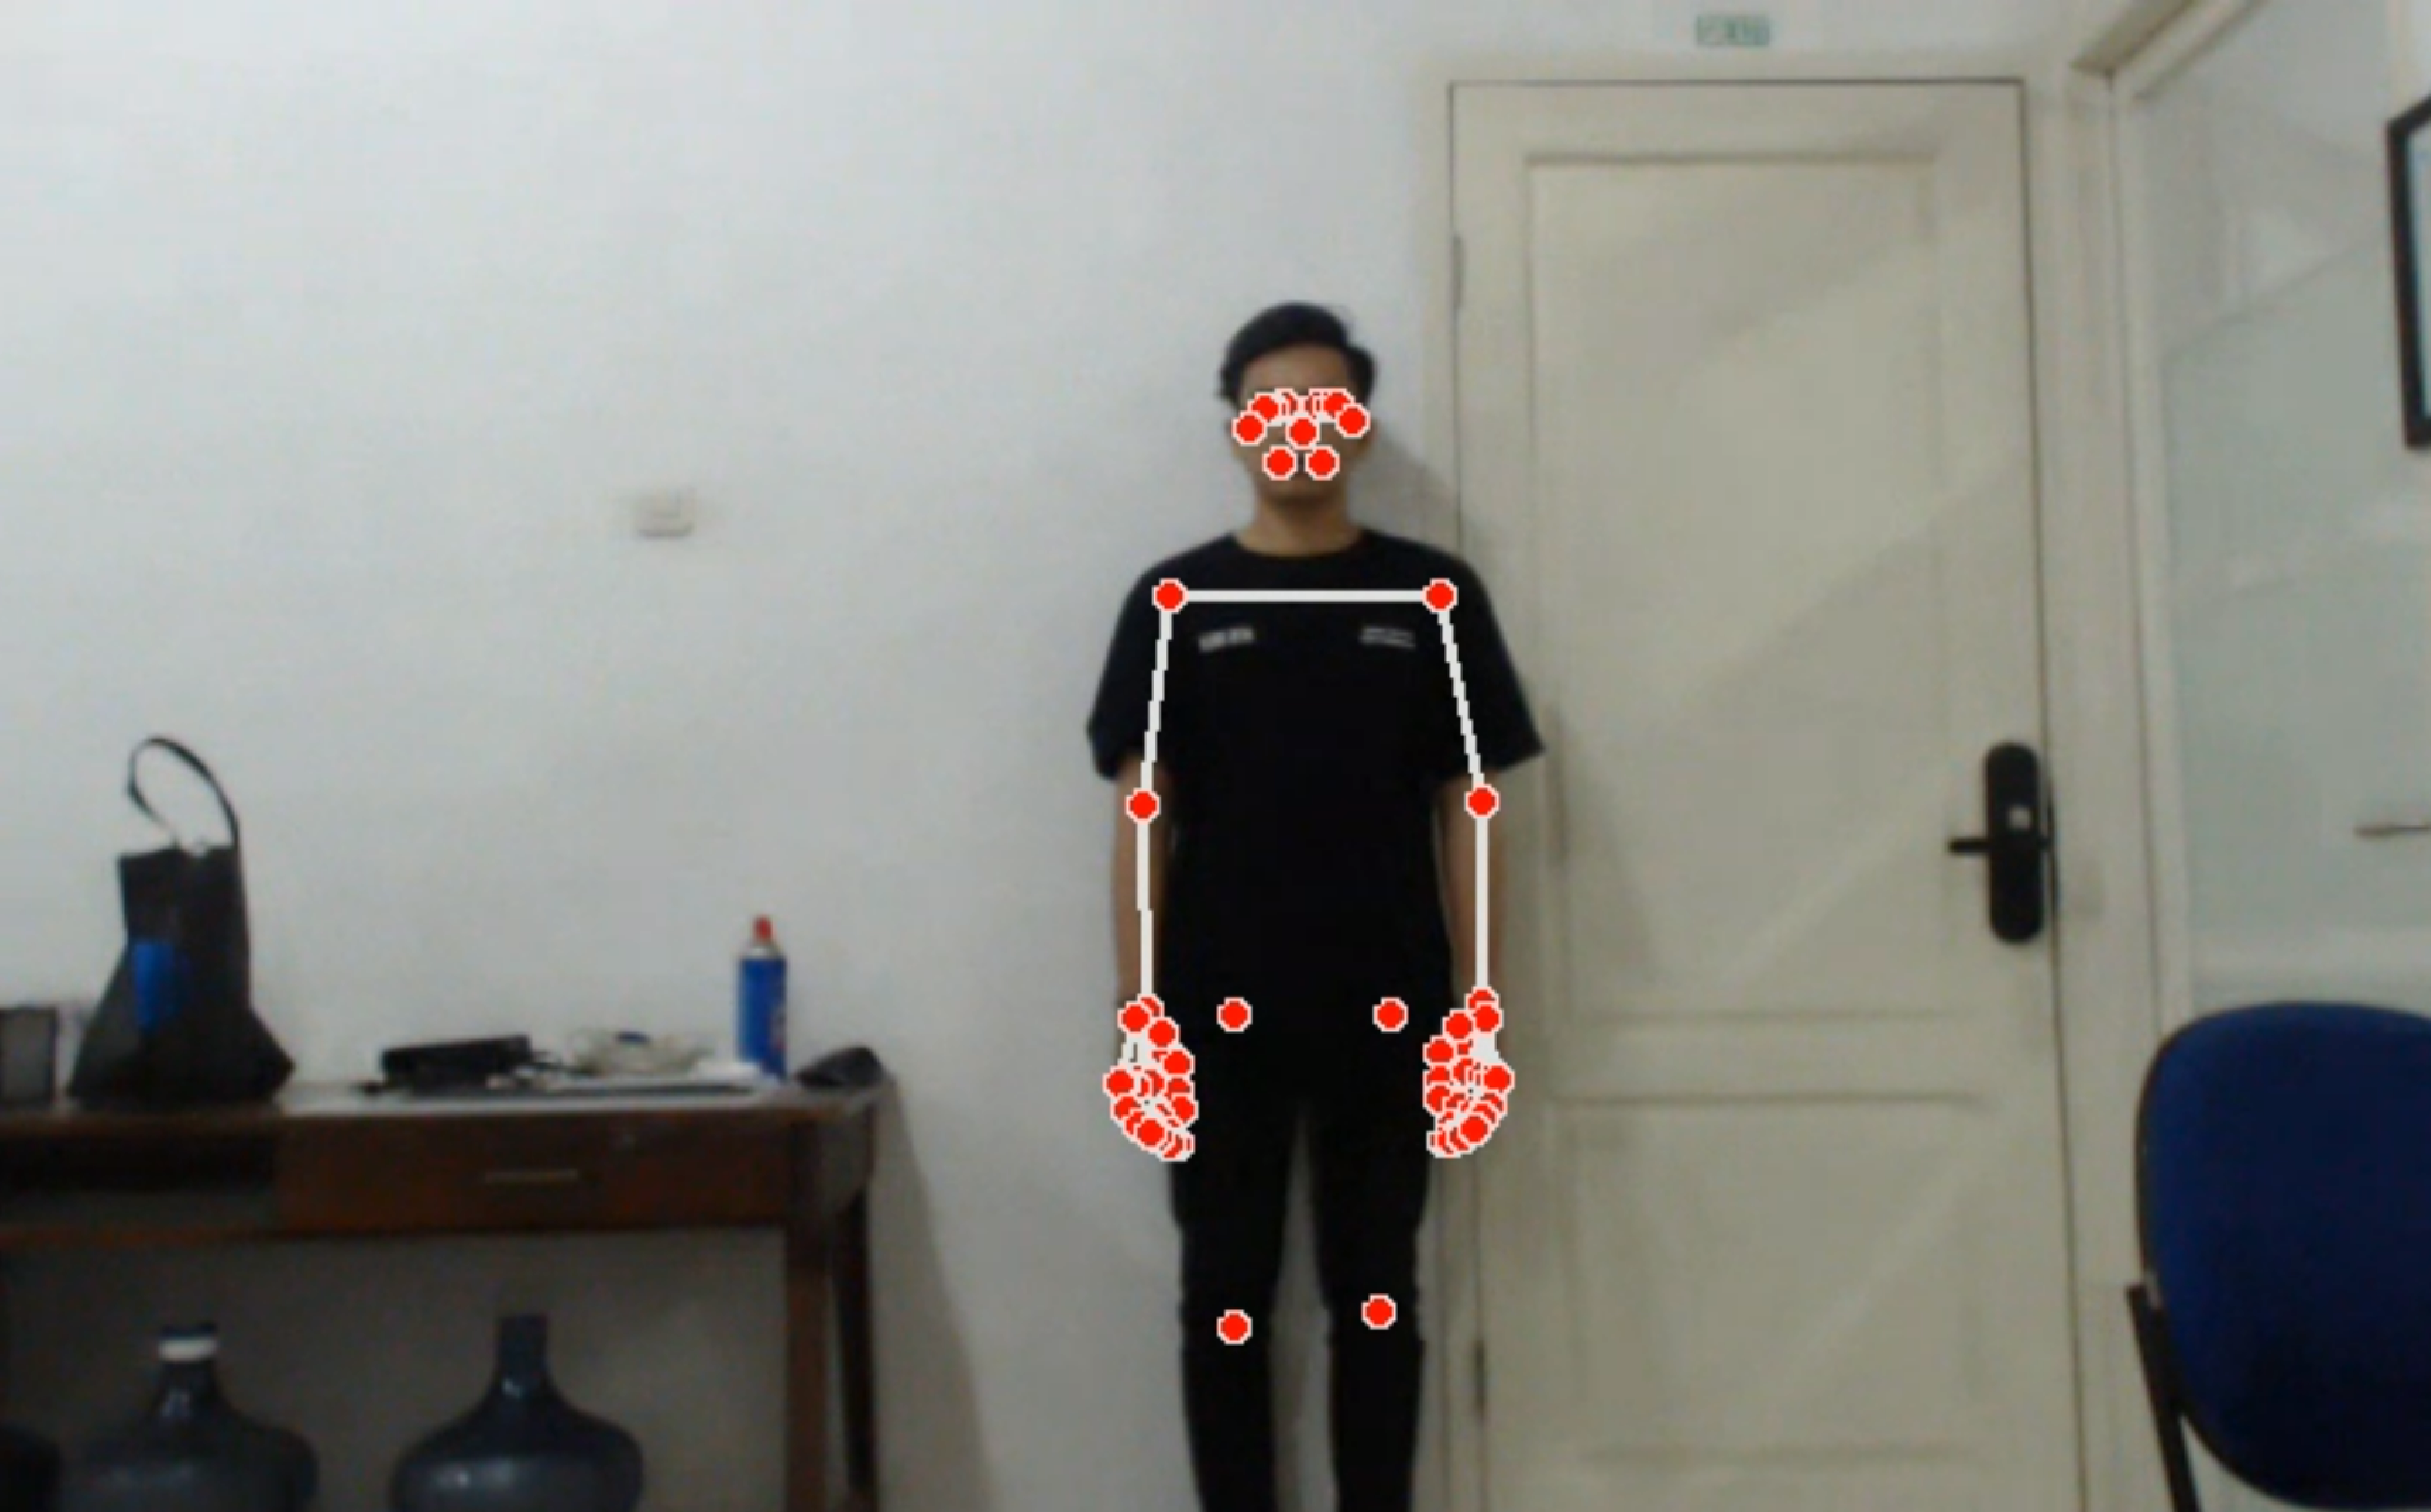
\includegraphics[scale=0.17]{gambar/bab4-jarak180.png}                 \\
  \hline
\end{longtable}

\newpage
\subsection{Pengujian Jarak 180 cm}
\label{sec:analisisjarak1}

\begin{longtable}{|c|c|c|c|c|}
  \caption{Pengujian Pertama Model di Kondisi Jarak 180 cm}
  \label{tb:prediksipendek1}                                   \\
  \hline
  \rowcolor[HTML]{C0C0C0}
  \textbf{Kosakata} & \textbf{Klasifikasi Model} & \textbf{\emph{Processing Time}} & \textbf{\emph{Complete Time}} & \textbf{\emph{FPS}}\\
  \hline
  Maaf              & Maaf                          & 0.09432 detik                           & 2.62625 detik                                 & 11.42311201\\
  Tolong            & Tolong                        & 0.09578 detik                           & 2.75824 detik                                 & 10.8764982\\
  Nama              & Nama                          & 0.09367 detik                           & 2.76423 detik                                 & 10.85294217\\
  Saya              & Saya                          & 0.09214 detik                           & 1.45957 detik                                 & 20.55396618\\
  Siapa             & Siapa                         & 0.09188 detik                           & 2.68606 detik                                 & 11.16875744\\
  Rumah             & \textcolor{red}{Delete}       & 0.09518 detik                           & 2.72404 detik                                 & 11.01303666\\
  Delete            & Delete                        & 0.09379 detik                           & 1.47150 detik                                 & 20.38732131\\
  Standby           & Standby                       & 0.09064 detik                           & 1.40810 detik                                 & 21.30526701\\
  Translate         & Translate                     & 0.09036 detik                           & 2.90195 detik                                 & 10.33787667\\
  \hline
\end{longtable}


\begin{longtable}{|c|c|c|c|c|}
  \caption{Pengujian Kedua Model di Kondisi Jarak 180 cm}
  \label{tb:prediksipendek2}                                   \\
  \hline
  \rowcolor[HTML]{C0C0C0}
  \textbf{Kosakata} & \textbf{Klasifikasi Model} & \textbf{\emph{Processing Time}} & \textbf{\emph{Complete Time}} & \textbf{\emph{FPS}}\\
  \hline
  Maaf              & \textcolor{red}{Tolong}       & 0.10251 detik                           & 2.68328 detik                                 & 11.18033853\\
  Tolong            & Tolong                        & 0.10531 detik                           & 2.67619 detik                                 & 11.20998081\\
  Nama              & Nama                          & 0.10347 detik                           & 2.83800 detik                                 & 10.57082874\\
  Saya              & Saya                          & 0.10078 detik                           & 1.60659 detik                                 & 18.67313694\\
  Siapa             & Siapa                         & 0.09793 detik                           & 2.89107 detik                                 & 10.37677789\\
  Rumah             & Rumah                         & 0.09961 detik                           & 2.97634 detik                                 & 10.07950553\\
  Delete            & Delete                        & 0.10204 detik                           & 1.43186 detik                                 & 20.95172062\\
  Standby           & Standby                       & 0.10917 detik                           & 1.42540 detik                                 & 21.04676217\\
  Translate         & Translate                     & 0.10983 detik                           & 3.00642 detik                                 & 9.978645248\\
  \hline
\end{longtable}


\begin{longtable}{|c|c|c|c|c|}
  \caption{Pengujian Ketiga Model di Kondisi Jarak 180 cm}
  \label{tb:prediksipendek3}                                   \\
  \hline
  \rowcolor[HTML]{C0C0C0}
  \textbf{Kosakata} & \textbf{Klasifikasi Model} & \textbf{\emph{Processing Time}} & \textbf{\emph{Complete Time}} & \textbf{\emph{FPS}}\\
  \hline
  Maaf              & Maaf                          & 0.09704 detik                           & 2.60797 detik                                 & 11.50321979\\
  Tolong            & Tolong                        & 0.11110 detik                           & 2.68802 detik                                 & 11.16064415\\
  Nama              & Nama                          & 0.11300 detik                           & 2.85448 detik                                 & 10.50980117\\
  Saya              & Saya                          & 0.10576 detik                           & 1.40619 detik                                 & 21.33420142\\
  Siapa             & Siapa                         & 0.10793 detik                           & 2.81908 detik                                 & 10.64176832\\
  Rumah             & Rumah                         & 0.10235 detik                           & 2.89943 detik                                 & 10.34685349\\
  Delete            & Delete                        & 0.10875 detik                           & 1.38759 detik                                 & 21.62023516\\
  Standby           & Standby                       & 0.11035 detik                           & 1.39657 detik                                 & 21.48127055\\
  Translate         & Translate                     & 0.10169 detik                           & 3.11065 detik                                 & 9.644273064\\
  \hline
\end{longtable}


Berdasarkan tiga pengujian yang dilakukan, didapatkan bahwa hampir keseluruhan klasifikasi model yang sesuai dengan \emph{class} kosakata. Namun, terdapat beberapa kesalahan model dalam melakukan klasifikasi. Dapat dilihat pada tabel \ref{tb:prediksipendek1} untuk isyarat kosakata "Rumah" diklasifikasikan sebagai "Delete" dan pada tabel \ref{tb:prediksipendek2} untuk isyarat kosakata "Maaf" diklasifikasikan sebagai "Tolong". Adanya kemiripan antara kosakata menjadi penyebab utama terjadinya kesalahan ini. Kosakata "Rumah" dan "Delete" memiliki kemiripan pada gerakan isyaratnya, dimana kedua kosakata ini sama - sama menggunakan dua tangan dengan gerakan yang mayoritas terjadi pada bagian badan pengguna. Sedangkan untuk kosakata "Maaf" dan "Tolong" memiliki kemiripan pada gerakan isyaratnya dengan kedua kosakata sama - sama menggunakan tangan kanan dengan gerakan akhir yang mayoritas terjadi pada bagian samping wajah pengguna. Namun kemiripan ini tidak sepenuhnya membuat hasil klasifikasi menjadi lebih condong ke suatu kosakata, melainkan dengan pengguna yang memperagakan bahasa isyarat dengan mengutamakan "ciri khas" dari masing - masing bahasa isyarat dapat menghasilkan hasil klasifikasi model yang baik. Hal ini dapat dilihat pada tabel \ref{tb:prediksipendek2} menghasilkan keseluruhan klasifikasi yang benar untuk seluruh \emph{class} kosakata. Pada pengujian dengan kondisi jarak 180 cm, berdasarkan data pda tabel \ref{tb:prediksipendek1}, tabel tabel \ref{tb:prediksipendek2}, dan tabel tabel \ref{tb:prediksipendek3} menunjukkan bahwa model memiliki akurasi klasifikasi sebesar 92.5\%.

Apabila dilihat berdasarkan waktu pemrosesan, rata - rata waktu yang dibutuhkan model untuk menghasilkan klasifikasi bahasa isyarat (\emph{processing time}) adalah 0.101 detik dan rata - rata waktu yang dibutuhkan dalam menghasilkan klasifikasi bahasa isyarat (\emph{complete time}) adalah 2.352 detik. Berdasakan data ini, dapat diamati bahwa model memerlukan waktu yang terbilang singkat dalam memproses serangkaian data koordinat yang diberikan dengan program penerjemah yang mampu menyelesaikan proses klasifikasi dengan cepat untuk sistem yang berjalan secara \emph{real time}. Adapun untuk nilai rata - rata FPS berdasarkan 3 pengujian yang dilakukan adalah 14.083. Meskipun dengan kondisi pengguna yang memiliki jarak yang cukup dekat dengan kamera, tidak mempengaruhi secara signifikan terhadap proses klasifikasi bahasa isyarat yang dilakukan oleh model.

Pada pengujian di kondisi jarak 180 cm ini, perlu diperhatikan bahwa pengguna harus melakukan gerakan bahasa isyarat dengan memastikan bahwa bagian tubuh kepala hingga tangan dengan jelas terlihat. Hal ini sangat krusial karena model memerlukan informasi koordinat yang lengkap untuk setiapp gerakan isyarat sehingga dapat menghasilkan klasifikasi yang tepat. Terkhususnya untuk kosakata "Translate", "Maaf", "Tolong", dan "Delete" yang memiliki gerakan isyarat yang cukup dinamis dan mayoritas gerakannya terjadi di samping kepala pengguna.  

\subsection{Pengujian Jarak 240 cm}
\label{sec:analisisjarak2}

\begin{longtable}{|c|c|c|c|c|}
  \caption{Pengujian Pertama Model di Kondisi Jarak 240 cm}
  \label{tb:prediksitengah1}                                   \\
  \hline
  \rowcolor[HTML]{C0C0C0}
  \textbf{Kosakata} & \textbf{Klasifikasi Model} & \textbf{\emph{Processing Time}} & \textbf{\emph{Complete Time}} & \textbf{\emph{FPS}}\\
  \hline
  Maaf              & Maaf                          & 0.09363 detik                           & 2.86369 detik                                  & 10.47599114\\
  Tolong            & Tolong                        & 0.09594 detik                           & 2.69973 detik                                  & 11.11221089\\
  Nama              & Nama                          & 0.09915 detik                           & 2.71606 detik                                  & 11.04540295\\
  Saya              & Saya                          & 0.09490 detik                           & 1.38486 detik                                  & 21.66277929\\
  Siapa             & Siapa                         & 0.09771 detik                           & 2.77829 detik                                  & 10.7980115\\
  Rumah             & Rumah                         & 0.09179 detik                           & 2.84222 detik                                  & 10.55513362\\
  Delete            & Delete                        & 0.09783 detik                           & 2.74689 detik                                  & 10.92144369\\
  Standby           & Standby                       & 0.09716 detik                           & 1.44449 detik                                  & 20.76861067\\
  Translate         & Translate                     & 0.09462 detik                           & 2.89943 detik                                  & 10.34685349\\
  \hline
\end{longtable}


\newpage
\begin{longtable}{|c|c|c|c|c|}
  \caption{Pengujian Kedua Model di Kondisi Jarak 240 cm}
  \label{tb:prediksitengah2}                                   \\
  \hline
  \rowcolor[HTML]{C0C0C0}
  \textbf{Kosakata} & \textbf{Klasifikasi Model} & \textbf{\emph{Processing Time}} & \textbf{\emph{Complete Time}} & \textbf{\emph{FPS}}\\
  \hline
  Maaf              & Maaf                          & 0.10063 detik                           & 2.83704 detik                                  & 10.57439991\\
  Tolong            & Tolong                        & 0.10465 detik                           & 2.74551 detik                                  & 10.926935\\
  Nama              & Nama                          & 0.07916 detik                           & 2.71480 detik                                  & 11.0505538\\
  Saya              & Saya                          & 0.11030 detik                           & 1.45698 detik                                  & 20.59049293\\
  Siapa             & Siapa                         & 0.09941 detik                           & 2.71764 detik                                  & 11.0389784\\
  Rumah             & Rumah                         & 0.10740 detik                           & 2.78343 detik                                  & 10.77806101\\
  Delete            & Delete                        & 0.10263 detik                           & 2.84822 detik                                  & 10.5328947\\
  Standby           & Standby                       & 0.10418 detik                           & 1.42558 detik                                  & 21.04412222\\
  Translate         & Translate                     & 0.10815 detik                           & 2.91372 detik                                  & 10.29610573\\
  \hline
\end{longtable}



\begin{longtable}{|c|c|c|c|c|}
  \caption{Pengujian Ketiga Model di Kondisi Jarak 240 cm}
  \label{tb:prediksitengah3}                                   \\
  \hline
  \rowcolor[HTML]{C0C0C0}
  \textbf{Kosakata} & \textbf{Klasifikasi Model} & \textbf{\emph{Processing Time}} & \textbf{\emph{Complete Time}} & \textbf{\emph{FPS}}\\
  \hline
  Maaf              & Maaf                          & 0.08161 detik                           & 2.93442 detik                                  & 10.22350162\\
  Tolong            & Tolong                        & 0.10857 detik                           & 2.84241 detik                                  & 10.55441648\\
  Nama              & Nama                          & 0.08474 detik                           & 2.87571 detik                                  & 10.43221665\\
  Saya              & Saya                          & 0.10568 detik                           & 1.77221 detik                                  & 16.92801072\\
  Siapa             & Siapa                         & 0.10201 detik                           & 2.62119 detik                                  & 11.4451809\\
  Rumah             & \textcolor{red}{Delete}       & 0.10468 detik                           & 2.72556 detik                                  & 11.00690965\\
  Delete            & Delete                        & 0.10309 detik                           & 2.82816 detik                                  & 10.60758815\\
  Standby           & Standby                       & 0.10799 detik                           & 1.42754 detik                                  & 21.01512639\\
  Translate         & Translate                     & 0.10627 detik                           & 2.81355 detik                                  & 10.66268053\\
  \hline
\end{longtable}




Berdasarkan tiga pengujian yang telah dilakukan, didapatkan bahwa hampir keseluruhan klasifikasi model telah sesuai dengan \emph{class} kosakata yang bersesuaian. Hal ini menunjukkan bahwa adanya pengaruh antara jarak pengguna dengan kamera terhadap proses klasifikasi model. Peningkatan jarak pengguna terhadap menghasilkan klasifikasi yang lebih baik. Namun, masih terdapat kesalahan yang dapat dilihat pada tabel \ref{tb:prediksitengah3}, yaitu isyarat kosakata "Rumah" diklasifikasikan sebagai "Delete". Sama seperti yang sudah dijelaskan pada pengujian di kondisi jarak 180 cm bahwa terdapat kemiripan antara kosakata "Rumah" dengan "Delete". Pada pengujian dengan kondisi jarak 240 cm ini, berdasarkan data pada tabel \ref{tb:prediksitengah1}, tabel \ref{tb:prediksitengah2}, dan tabel \ref{tb:prediksitengah3} menunjukkan bahwa model memiliki akurasi klasifikasi sebesar 96.3\%.

Apabila dilihat berdasarkan waktu pemrosesan, rata - rata waktu yang dibutuhkan model untuk menghasilkan klasifikasi bahasa isyarat (\emph{processing time}) adalah 0.099 detik dan rata - rata waktu yang dibutuhkan dalam menghasilkan klasifikasi bahasa isyarat (\emph{complete time}) adalah 2.506 detik. Apabila dibandingkan dengan pengujian sebelumnya (kondisi jarak 180 cm). Terdapat peningkatan pada nilai \emph{processing time} seiring dengan peningkatan jarak kamera dengan pengguna yaitu sebesar 0.002 detik. Sedangkan untuk nilai \emph{complete time} mengalami penurunan seiring dengan peningkatan jarak kamera dengan pengguna, yaitu sebesar 0.154 detik. Adapun rata - rata FPS yang didapatkan bernilai 12.866. Apabila dilihat dari pengujian sebelumnya, terdapat penurunan dari nilai rata - rata FPS ini. Hal ini dapat disebabkan oleh adanya pengaruh antara jarak pengguna dengan kamera terhadap bagaimana beban kerja kamera dalam menangkap tiap \emph{frame}.

\subsection{Pengujian Jarak 300 cm}
\label{sec:analisisjarak3}

\begin{longtable}{|c|c|c|c|c|}
  \caption{Pengujian Pertama Model di Kondisi Jarak 300 cm}
  \label{tb:prediksijauh1}                                   \\
  \hline
  \rowcolor[HTML]{C0C0C0}
  \textbf{Kosakata} & \textbf{Klasifikasi Model} & \textbf{\emph{Processing Time}} & \textbf{\emph{Complete Time}} & \textbf{\emph{FPS}}\\
  \hline
  Maaf              & Maaf                          & 0.09520 detik                           & 2.73861 detik                                  & 10.95444597\\
  Tolong            & Tolong                        & 0.09268 detik                           & 2.87873 detik                                  & 10.42125245\\
  Nama              & Nama                          & 0.09824 detik                           & 2.91580 detik                                  & 10.28878128\\
  Saya              & Saya                          & 0.09438 detik                           & 2.81194 detik                                  & 10.66878297\\
  Siapa             & Siapa                         & 0.10269 detik                           & 2.76496 detik                                  & 10.85005044\\
  Rumah             & Rumah                         & 0.09520 detik                           & 2.74032 detik                                  & 10.9476124\\
  Delete            & Delete                        & 0.09270 detik                           & 2.98108 detik                                  & 10.06347157\\
  Standby           & Standby                       & 0.09150 detik                           & 2.81312 detik                                  & 10.66433428\\
  Translate         & Translate                     & 0.09415 detik                           & 2.84808 detik                                  & 10.53339729\\
  \hline
\end{longtable}


\begin{longtable}{|c|c|c|c|c|}
  \caption{Pengujian Kedua Model di Kondisi Jarak 300 cm}
  \label{tb:prediksijauh2}                                   \\
  \hline
  \rowcolor[HTML]{C0C0C0}
  \textbf{Kosakata} & \textbf{Klasifikasi Model} & \textbf{\emph{Processing Time}} & \textbf{\emph{Complete Time}} & \textbf{\emph{FPS}}\\
  \hline
  Maaf              & Maaf                          & 0.11375 detik                           & 2.86339 detik                                  & 10.47709021\\
  Tolong            & Tolong                        & 0.10336 detik                           & 2.74577 detik                                  & 10.92588184\\
  Nama              & Nama                          & 0.10118 detik                           & 2.69010 detik                                  & 11.15200889\\
  Saya              & Saya                          & 0.11127 detik                           & 2.72032 detik                                  & 11.02812309\\
  Siapa             & Siapa                         & 0.10363 detik                           & 2.84954 detik                                  & 10.52800361\\
  Rumah             & Rumah                         & 0.10374 detik                           & 2.87114 detik                                  & 10.44879738\\
  Delete            & Delete                        & 0.10743 detik                           & 2.73295 detik                                  & 10.97715222\\
  Standby           & Standby                       & 0.10061 detik                           & 2.90372 detik                                  & 10.33158689\\
  Translate         & Translate                     & 0.10337 detik                           & 2.75235 detik                                  & 10.89978846\\
  \hline
\end{longtable}


\begin{longtable}{|c|c|c|c|c|}
  \caption{Pengujian Ketiga Model di Kondisi Jarak 300 cm}
  \label{tb:prediksijauh3}                                   \\
  \hline
  \rowcolor[HTML]{C0C0C0}
  \textbf{Kosakata} & \textbf{Klasifikasi Model} & \textbf{\emph{Processing Time}} & \textbf{\emph{Complete Time}} & \textbf{\emph{FPS}}\\
  \hline
  Maaf              & Maaf                          & 0.09520 detik                           & 2.75798 detik                                  & 10.87754186\\
  Tolong            & Tolong                        & 0.09268 detik                           & 2.66197 detik                                  & 11.26986055\\
  Nama              & Nama                          & 0.09824 detik                           & 2.88613 detik                                  & 10.39454784\\
  Saya              & Saya                          & 0.09438 detik                           & 2.80015 detik                                  & 10.7137212\\
  Siapa             & Siapa                         & 0.10269 detik                           & 2.76350 detik                                  & 10.85577924\\
  Rumah             & Rumah                          & 0.09520 detik                           & 2.81146 detik                                  & 10.67060149\\
  Delete            & Delete                        & 0.09270 detik                           & 2.69894 detik                                  & 11.11547971\\
  Standby           & Standby                       & 0.09675 detik                           & 2.75581 detik                                  & 10.88609619\\
  Translate         & Translate                     & 0.10323 detik                           & 2.67942 detik                                  & 11.19645498\\
  \hline
\end{longtable}



Berdasarkan tiga pengujian yang telah dilakukan, didapatkan bahwa keseluruhan klasifikasi model yang sesuai dengan \emph{class} kosakata. Hal ini menunjukkan bahwa peningkatan jarak berpengaruh pada proses klasifikasi yang dilakukan oleh model. Peningkatan jarak antara pengguna dengan kamera, terkhususnya pada jarak terjauh pada pengujian ini, menghasilkan klasifikasi yang lebih baik dan tepat sesuai dengan kosakata yang bersesuaian dengan gerakannya. Hal ini dapat disebabkan oleh semakin jauh jarak antara kamera dengan pengguna memudahkan dalam memproses pose pengguna sehingga menghasilkan data koordinat yang lebih baik lagi. Berdasarkan data pada tabel \ref{tb:prediksijauh1}, tabel \ref{tb:prediksijauh2}, tabel \ref{tb:prediksijauh3} menunjukkan bahwa model memiliki akurasi klasifikasi sebesar 100\%.

Apabila dilihat berdasarkan waktu pemrosesan, rata - rata waktu yang dibutuhkan model untuk menghasilkan klasifikasi bahasa isyarat (\emph{processing time}) adalah 0.099 detik dan rata - rata waktu yang dibutuhkan dalam menghasilkan klasifikasi bahasa isyarat (\emph{complete time}) adalah 2.794 detik. Dapat dilihat bahwa tidak terdapat peningkatan pada \emph{processing time} jika dibandingkan dengan variasi jarak pada pengujian sebelumnya. Namun, pada nilai \emph{complete time} terdapat penurunan jika dibandingkan dengan pengujian sebelumnya, yaitu sebesar 0.288 detik. Hal ini menunjukkan bahwa terdapat penurunan dari nilai \emph{complete time} seiring dengan peningkatan jarak kamera dengan pengguna. Adapun untuk nilai rata - rata FPS yang didapatkan berdasarkan 3 pengujian yang telah dilakukan bernilai 10.746. Apabila dibandingkan dengan pengujian - pengujian sebelumnya, terdapat penurunan pada nilai rata - rata FPS ini. Hal ini dapat kembali lagi menguatkan bahwa adanya pengaruh antara jarak pengguna dengan kamera terhadap bagaimana beban kerja kamera dalam menangkap tiap \emph{frame}, dimana adanya peningkatan jarak menghasilkan model yang lebih baik dalam melakukan klasifikasi, namun dengan beban kerja yang lebih berat bagi sistem secara keseluruhan.

\subsection{Rangkuman Pengujian Kondisi Jarak}
\label{sec:analisisrangkumanjarak}

\begin{longtable}{|c|c|c|c|c|}
  \caption{Rangkuman Pengujian Kondisi Jarak}
  \label{tb:evaluasiJarak}                                   \\
  \hline
  \rowcolor[HTML]{C0C0C0}
  \textbf{Jarak} & \textbf{Akurasi} & \emph{\textbf{Avg. Processing Time}} & \emph{\textbf{Avg. Complete Time}} & \emph{FPS}\\
  \hline
  180 cm & 0.89 & 0.1017 detik & 2.3660 detik & 14.083\\
  240 cm & 0.96 & 0.0994 detik & 2.5098 detik & 12.866\\
  300 cm & 1.00 & 0.0997 detik & 2.7918 detik & 10.746\\
  \hline
\end{longtable}

Secara keseluruhan, dapat dilihat pada tabel \ref{tb:evaluasiJarak} bahwa variasi jarak yang berbeda tidak berpengaruh secara signifikan terhadap hasil klasifikasi model. Hal ini menunjukkan bahwa metode normalisasi data yang digunakan telah berhasil menghasilkan model yang invarian terhadap jarak. Dengan catatan bahwa posisi pengguna (terkhususnya bagian kepala dan tangan) dapat dengan jelas terlihat ketika melakukan gerakan isyarat. Dapat dilihat bahwa ada relasi antara jarak dengan \emph{average complete time}. Peningkatan \emph{average}. Namun, pada nilai \emph{average processing time} cenderung menurun dengan adanya peningkatan jarak. Kemampuan kamera dalam menangkap \emph{frame} menjadi pengaruh utama dalam peningkatan nilai \emph{complete time} dan \emph{processing time} karena gerakan isyarat yang dinamis memerlukan posisi kamera yang dapat menangkap setiap gerakan dengan jelas dan tepat. Semakin jelas gerakan isyarat yang ditangkap akan memudahkan \emph{framework} Mediapipe dalam mendapatkan data koordinat berdasarkan \emph{landmark} yang ada. Hal ini tentunya akan meningkatkan akurasi klasifikasi model, dimana ditunjukkan dengan adanya peningkatan akurasi seiring dengan peningkatan jarak. Adapun pada nilai rata - rata FPS mengalami penurunan seiring dengan peningkatan jarak antara pengguna dengan kamera. Hal ini menunjukkan bahwa sistem memiliki beban kerja yang lebih berat seiring dengan peningkatan jarak.

\newpage
\section{Pengujian Subjek Berbeda}
\label{sec:analisissubjek}

\begin{longtable}{|c|c|}
  \caption{Variasi Subjek Berbeda}
  \label{tb:kondisisubjek}                                   \\
  \hline
  \rowcolor[HTML]{C0C0C0}
  \textbf{Jenis Kelamin} & \textbf{Gambar Subjek}  \\
  \hline
  Perempuan              &  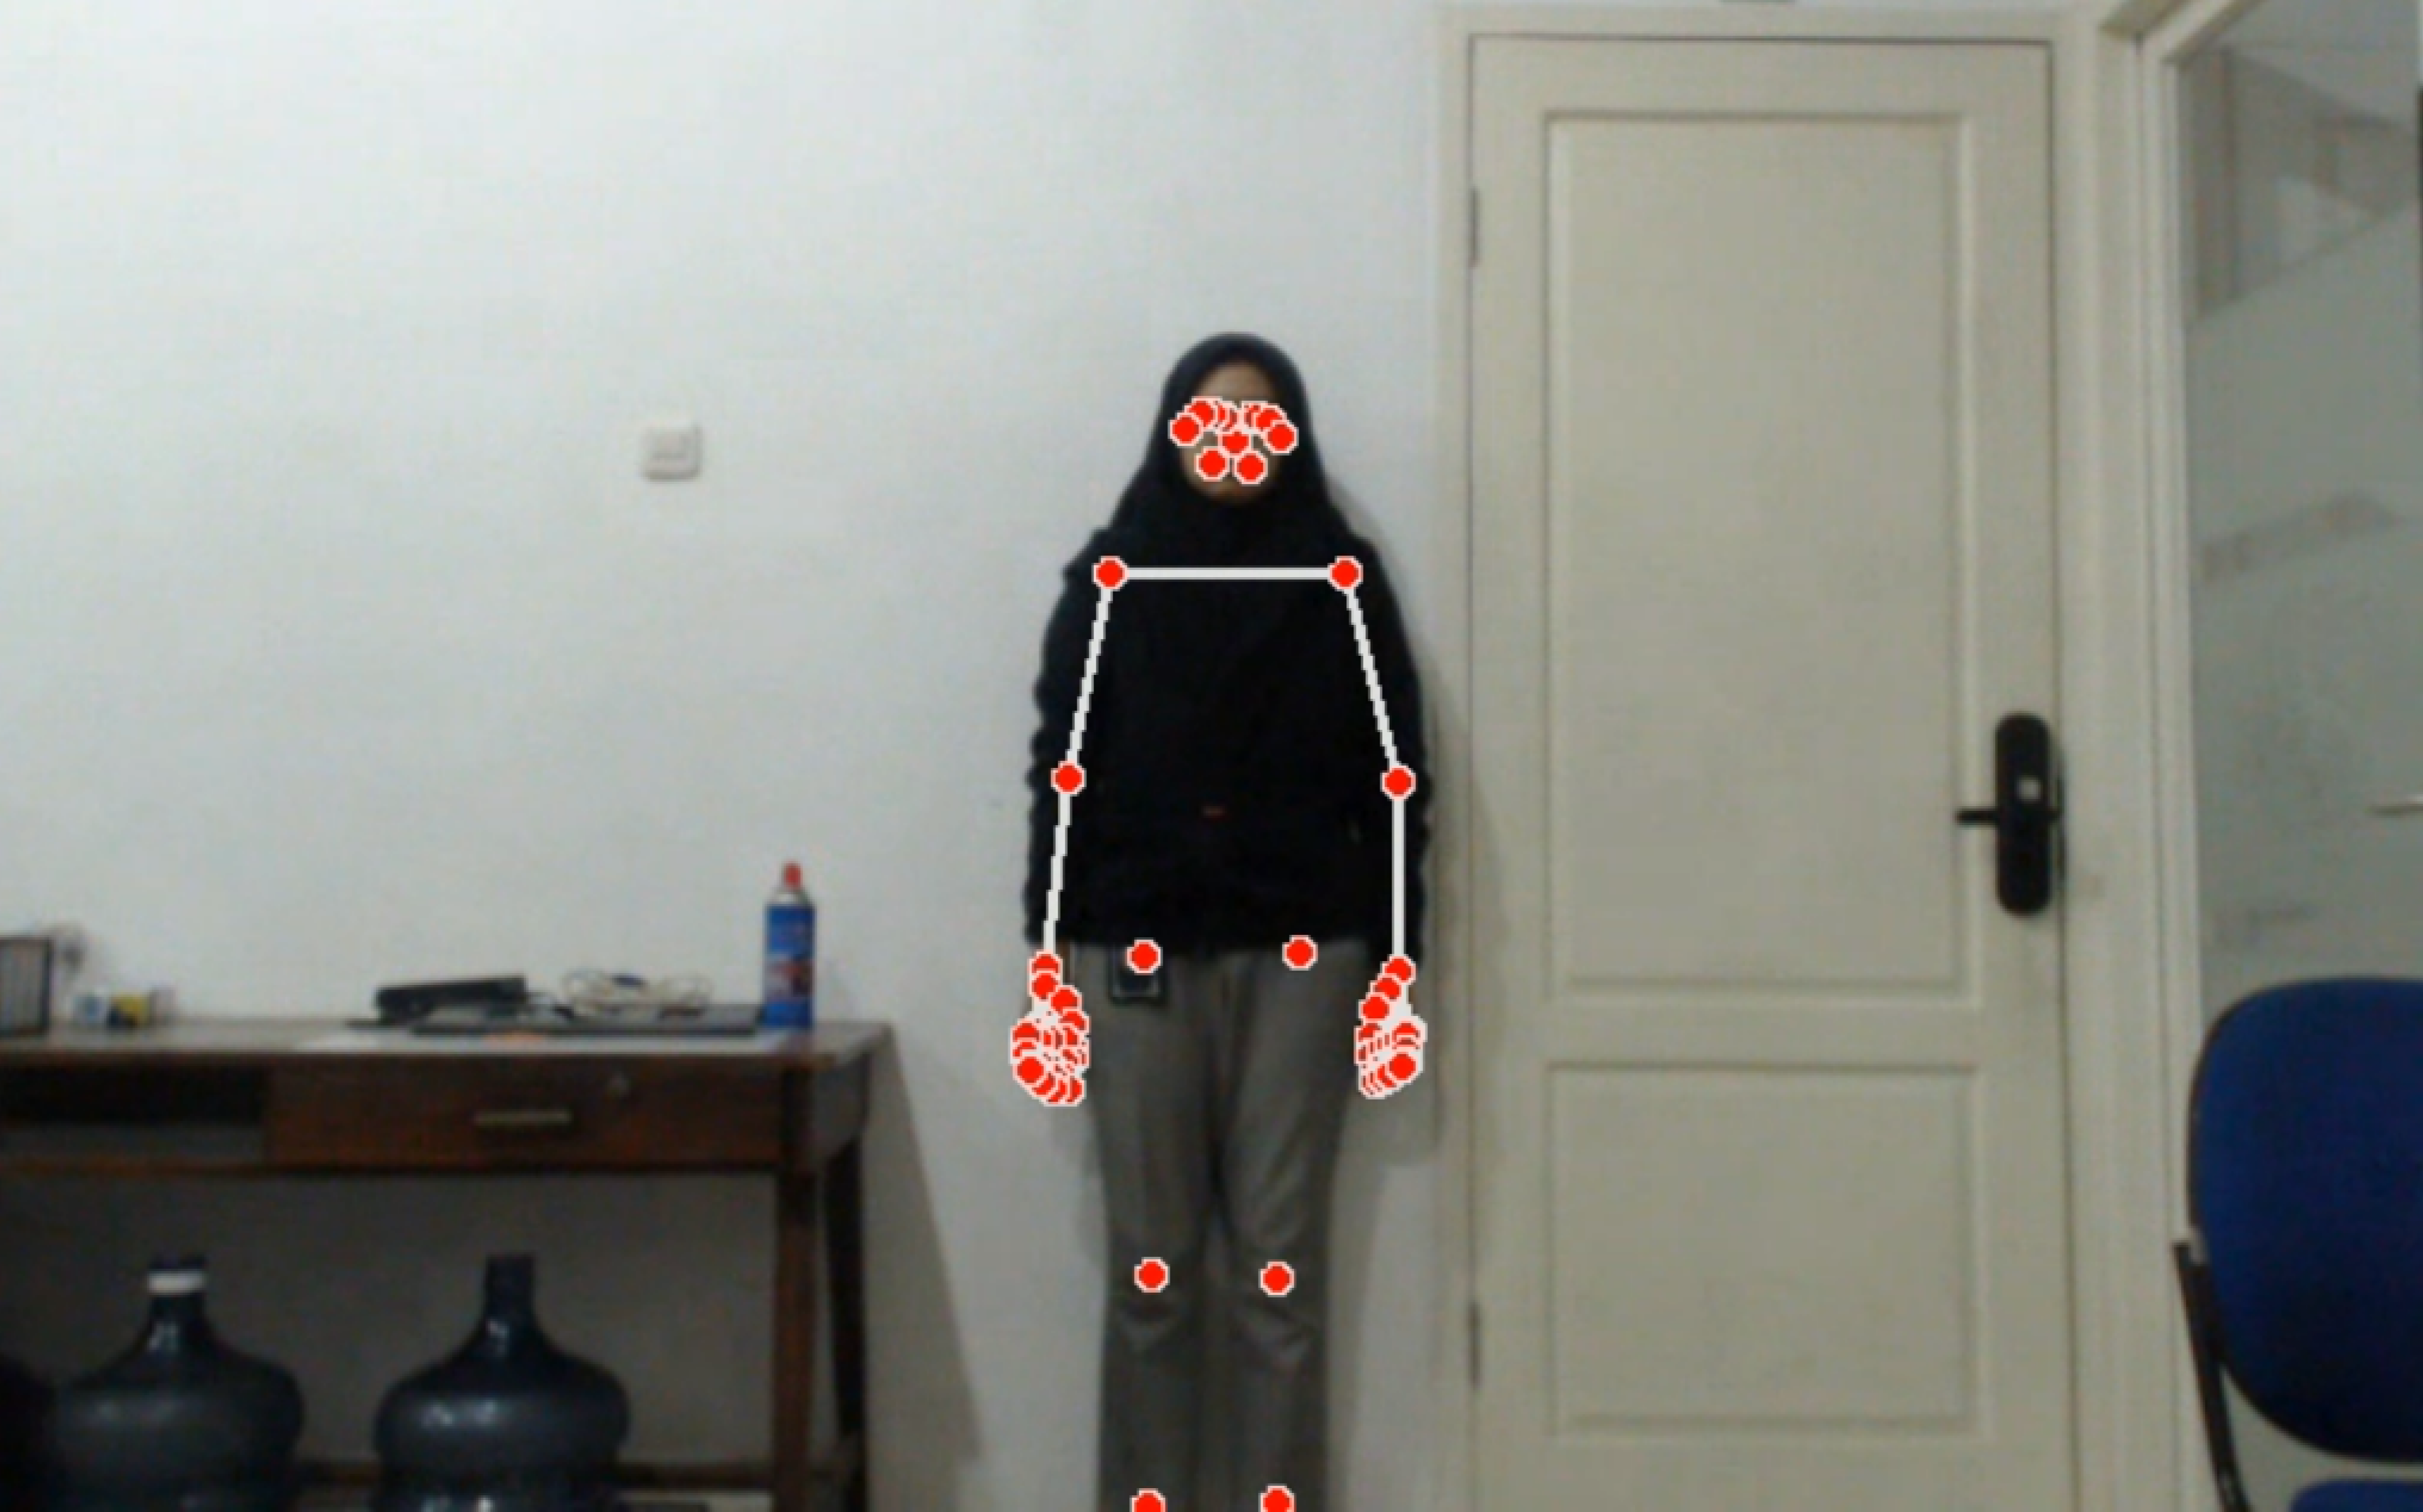
\includegraphics[scale=0.3]{gambar/bab4-rani.png}                \\
  \hline
  Laki - Laki            & 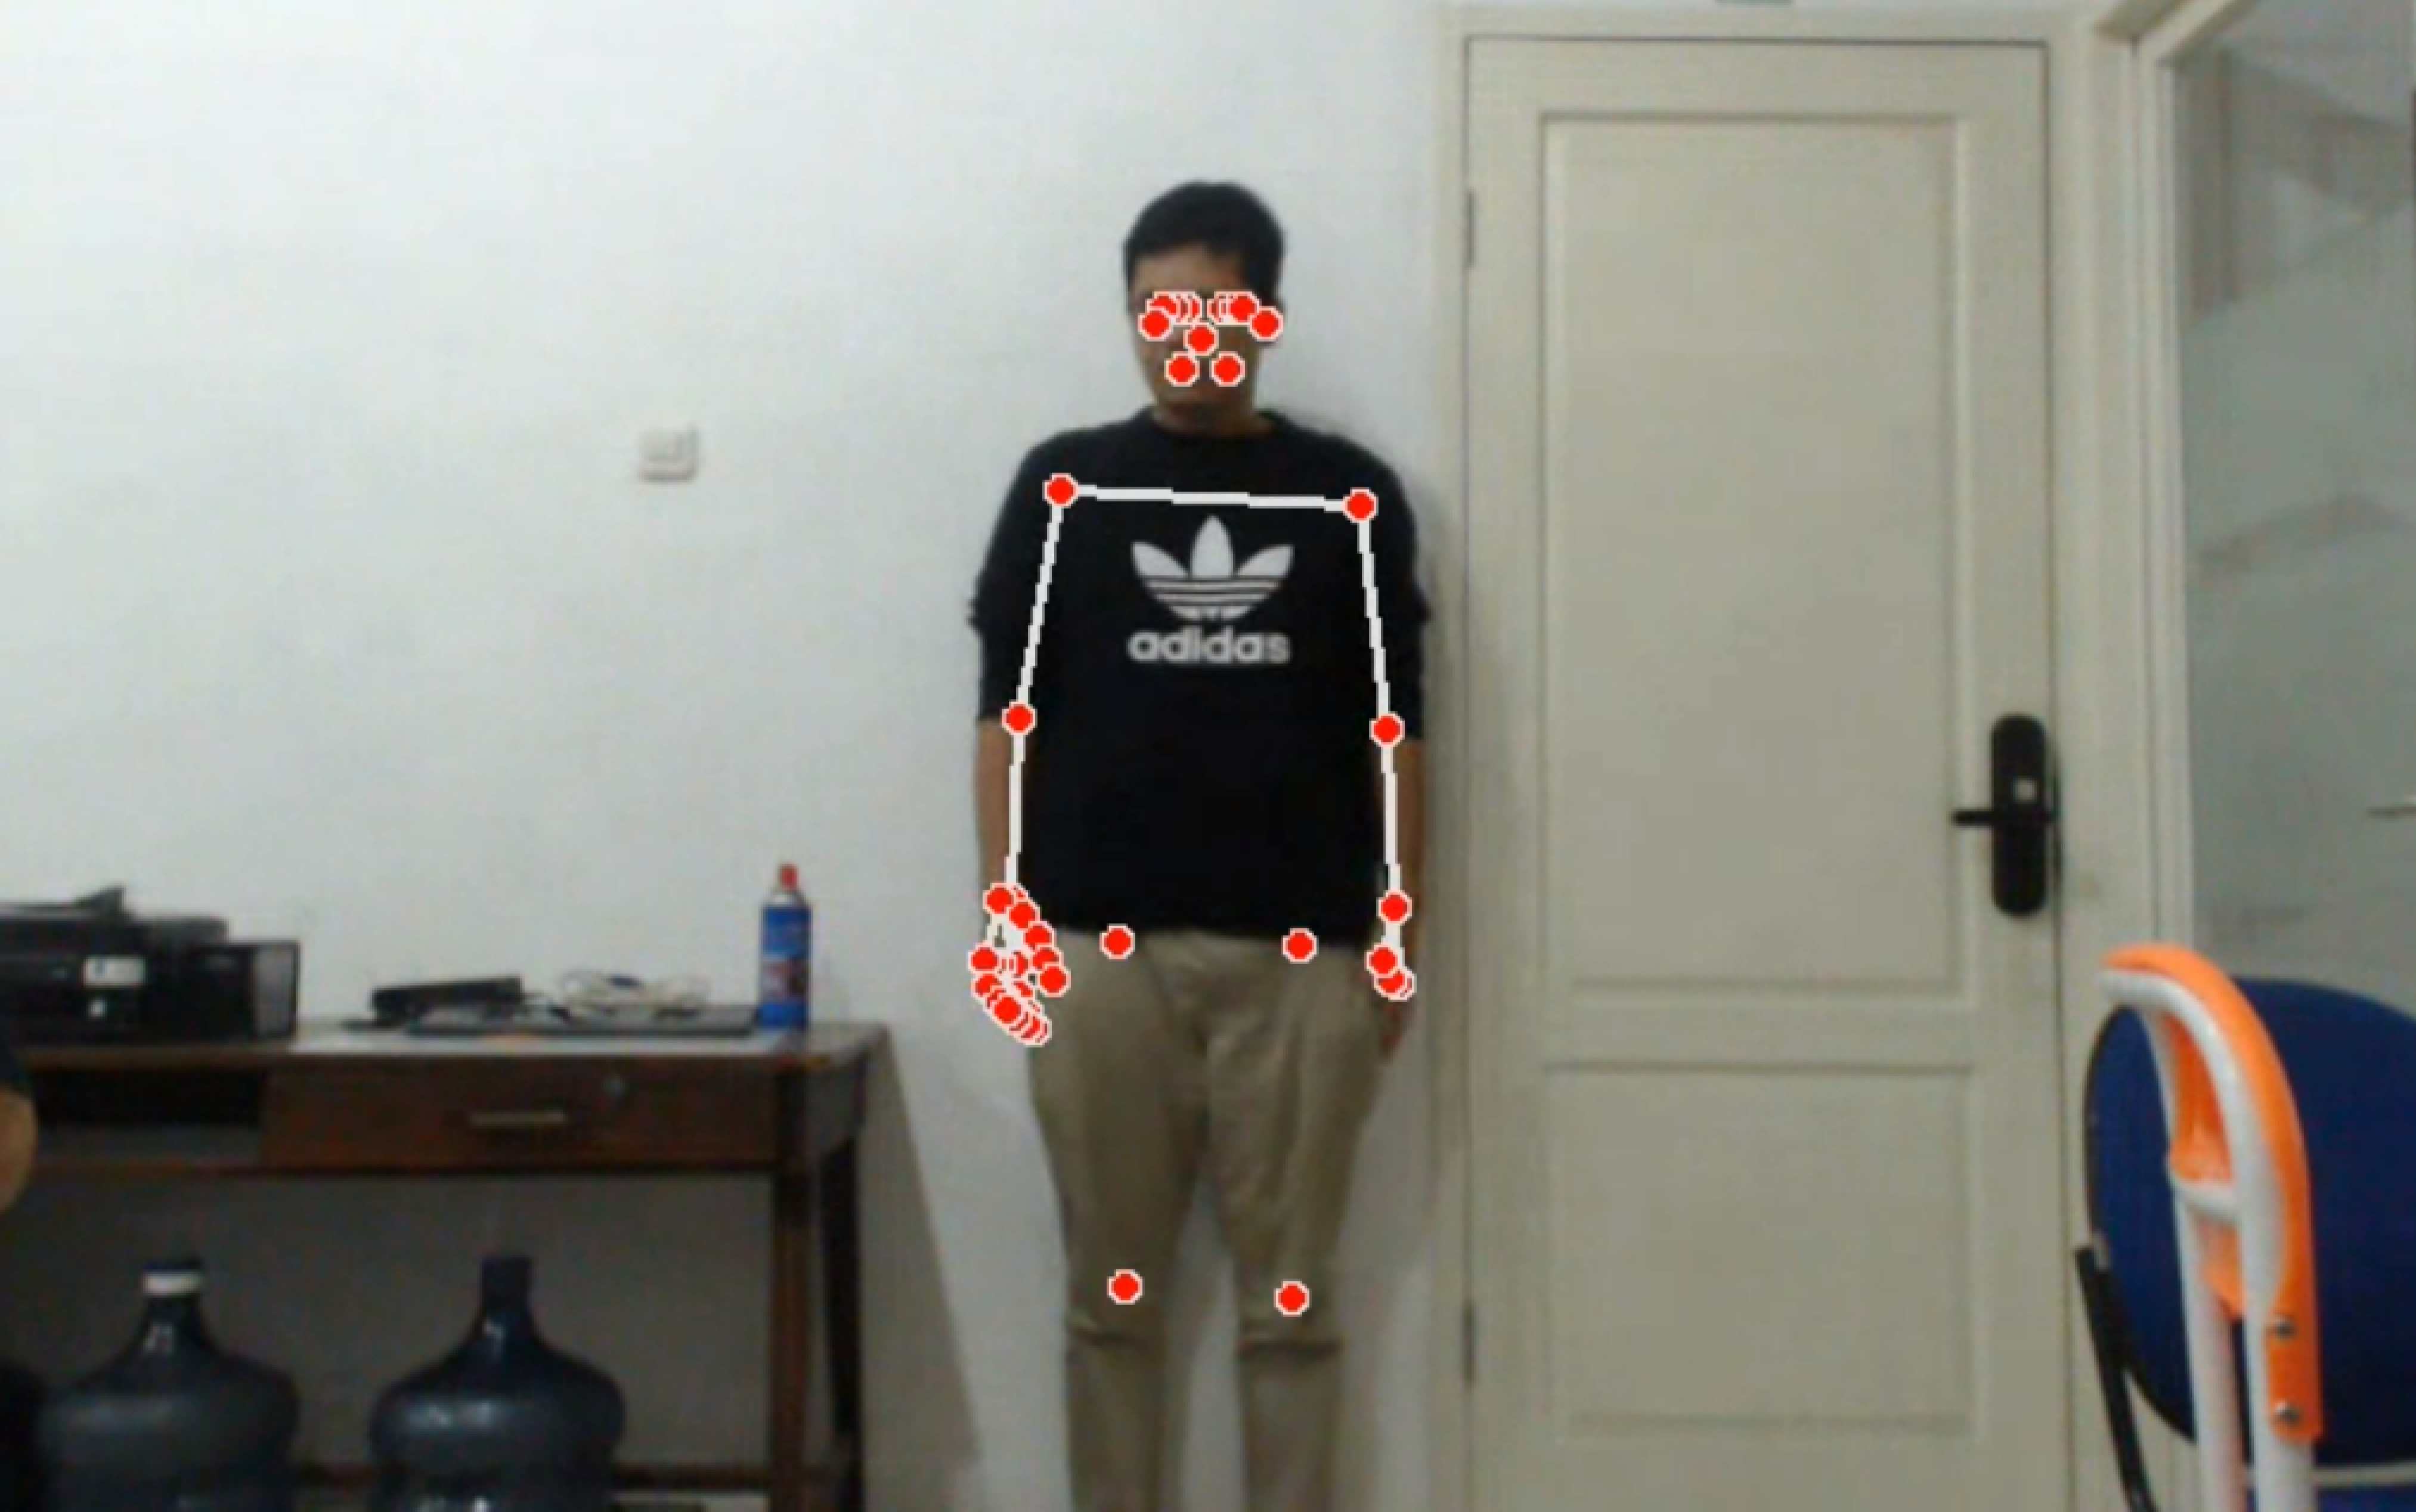
\includegraphics[scale=0.3]{gambar/bab4-evan.png}                 \\
  \hline
\end{longtable}

Pada pengujian dengan menggunakan subjek yang berbeda ini dilakukan untuk memahami bagaimana performa model pada pengguna selain darii penulis. Hal ini dilakukan demi melihat apakah model berhasil beradaptasi terhadap data yang bukan merupakan dataset yang digunakan dalam \emph{training} sehingga kedepannya dapat digunakan oleh kalangan luas. Adapun subjek yang akan diujikan berjumlah 2, yaitu 1 perempuan dan 1 laki - laki. Adapun gambaran subjek yang akan diujikan dapat dilihat pada tabel \ref{tb:kondisisubjek}. 

Model penerjemah bahasa Indonesia (BISINDO) yang akan digunakan pada pengujian ini adalah model pada bagian \ref{sec:analisismodel3} karena merupakan model yang menghasilkan klasifikasi yang terbaik jika dibandingkan dengan model lainnya. Untuk setiap intensitas cahaya akan dilakukan pengujian sebanyak tiga kali dengan jarak terhadap kamera sebesar 300 cm dan intensitas cahaya yang berkisar pada nilai 125 lux atau kondisi ruangan terang. Pada setiap pengujian akan dicari hasil klasifikasi model, waktu yang dibutuhkan model untuk menghasilkan klasifikasi bahasa isyarat berdasarkan data koordinat yang diberikan(\emph{processing time}), waktu total yang dibutuhkan dalam menghasilkan klasifikasi bahasa isyarat (\emph{complete time}), dan rata - rata FPS (\emph{frame per second}) yang didapatkan ketika proses klasifikasi dilakukan pada website.  

\subsection{Pengujian Subjek Perempuan}
\label{sec:analisisperempuan}

\begin{longtable}{|c|c|c|c|c|}
  \caption{Pengujian Pertama Model di Subjek Berbeda Perempuan}
  \label{tb:prediksiperempuan1}                                   \\
  \hline
  \rowcolor[HTML]{C0C0C0}
  \textbf{Kosakata} & \textbf{Klasifikasi Model} & \textbf{\emph{Processing Time}} & \textbf{\emph{Complete Time}} & \textbf{\emph{FPS}}\\
  \hline
  Maaf              & \textcolor{red}{Tolong}       & 0.09316 detik                           & 3.20865 detik                                  & 9.349722025\\
  Tolong            & Tolong                        & 0.09346 detik                           & 2.87486 detik                                  & 10.43527934\\
  Nama              & Nama                          & 0.09218 detik                           & 3.25495 detik                                  & 9.216731308\\
  Saya              & Saya                          & 0.09530 detik                           & 3.12871 detik                                  & 9.588624336\\
  Siapa             & Siapa                         & 0.09518 detik                           & 2.93024 detik                                  & 10.23807536\\
  Rumah             & \textcolor{red}{Delete}       & 0.10196 detik                           & 3.01911 detik                                  & 9.936707241\\
  Delete            & Delete                        & 0.10392 detik                           & 3.05715 detik                                  & 9.813073792\\
  Standby           & Standby                       & 0.09530 detik                           & 1.47974 detik                                  & 20.27379727\\
  Translate         & Translate                     & 0.09317 detik                           & 2.94322 detik                                  & 10.19291748\\
  \hline
\end{longtable}



\begin{longtable}{|c|c|c|c|c|}
  \caption{Pengujian Kedua Model di Subjek Berbeda Perempuan}
  \label{tb:prediksiperempuan2}                                   \\
  \hline
  \rowcolor[HTML]{C0C0C0}
  \textbf{Kosakata} & \textbf{Klasifikasi Model} & \textbf{\emph{Processing Time}} & \textbf{\emph{Complete Time}} & \textbf{\emph{FPS}}\\
  \hline
  Maaf              & Maaf                          & 0.09658 detik                           & 3.10876 detik                                  & 9.650153232\\
  Tolong            & Tolong                        & 0.09834 detik                           & 2.89284 detik                                  & 10.37041506\\
  Nama              & Nama                          & 0.09465 detik                           & 2.98028 detik                                  & 10.06617659\\
  Saya              & Saya                          & 0.09416 detik                           & 2.92525 detik                                  & 10.2555235\\
  Siapa             & Siapa                         & 0.09781 detik                           & 2.92773 detik                                  & 10.24682955\\
  Rumah             & Rumah                         & 0.09567 detik                           & 3.06411 detik                                  & 9.790762709\\
  Delete            & Delete                        & 0.10792 detik                           & 3.37185 detik                                  & 8.897189125\\
  Standby           & Standby                       & 0.09644 detik                           & 1.53859 detik                                  & 19.49841476\\
  Translate         & Translate                     & 0.10363 detik                           & 2.96890 detik                                  & 10.10473568\\
  \hline
\end{longtable}



\begin{longtable}{|c|c|c|c|c|}
  \caption{Pengujian Ketiga Model di Subjek Berbeda Perempuan}
  \label{tb:prediksiperempuan3}                                   \\
  \hline
  \rowcolor[HTML]{C0C0C0}
  \textbf{Kosakata} & \textbf{Klasifikasi Model} & \textbf{\emph{Processing Time}} & \textbf{\emph{Complete Time}} & \textbf{\emph{FPS}}\\
  \hline
  Maaf              & Maaf                          & 0.09668 detik                           & 3.10362 detik                                  & 9.666143525\\
  Tolong            & Tolong                        & 0.09738 detik                           & 3.04991 detik                                  & 9.836340227\\
  Nama              & Nama                          & 0.09641 detik                           & 2.92788 detik                                  & 10.24632891\\
  Saya              & Saya                          & 0.09479 detik                           & 1.46574 detik                                  & 20.46750762\\
  Siapa             & Siapa                         & 0.09821 detik                           & 3.08167 detik                                  & 9.734997029\\
  Rumah             & Rumah                         & 0.09820 detik                           & 2.87077 detik                                  & 10.45015111\\
  Delete            & Delete                        & 0.11417 detik                           & 3.02126 detik                                  & 9.929626447\\
  Standby           & Standby                       & 0.09473 detik                           & 1.54900 detik                                  & 19.36732451\\
  Translate         & Translate                     & 0.09833 detik                           & 3.12762 detik                                  & 9.591957427\\
  \hline
\end{longtable}



Berdasarkan tiga pengujian yang telah dilakukan, didapatkan bahwa hampir keseluruhan klasifikasi model yang sesuai dengan \emph{class} kosakata. Namun, terdapat beberapa kesalahan model dalam melakukan klasifikasi. Dapat dilihat pada tabel \ref{tb:prediksiperempuan1} untuk isyarat kosakata "Maaf" diklasifikasikan sebagai "Tolong". Hal ini dapat disebabkan oleh kesalahan pola gerakan isyarat yang digunakan, dimana kurang ditekankannya keunikan atau \emph{feature} dari masing - masing gerakan bahasa isyarat.  Secara garis besar, hasil pengujian ini menunjukkan bahwa model dengan mudah dapat mengklasifikasikan bahasa isyarat yang diperagakan oleh pengguna dengan jenis kelamin perempuan dengan akurasi sebesar 92.5\%. 

Apabila dilihat berdasarkan waktu pemrosesan, rata - rata waktu yang dibutuhkan model untuk menghasilkan klasifikasi bahasa isyarat (\emph{processing time}) adalah 0.098 detik dan rata - rata waktu yang dibutuhkan dalam menghasilkan klasifikasi bahasa isyarat (\emph{complete time}) adalah 2.810 detik. Hal ini menunjukkan bahwa pada subjek perempuan yang berbeda dengan penulis tidak mempengaruhi nilai \emph{processing time} dan \emph{complete time}. Adapun rata - rata nilai FPS yang didapatkan berdasarkan pengujian yang dilakukan bernilai 11.378. Nilai menunjukkan bahwa subjek perempuan yang berbeda dengan penulis tidak berpengaruh secara signifikan terhadap sistem yang ada. Hal ini juga menguatkan bahwa model telah dapat beradaptasi dengan subjek yang berbeda dengan penulis.

\subsection{Pengujian Subjek Laki - Laki}
\label{sec:analisislaki}

\begin{longtable}{|c|c|c|c|c|}
  \caption{Pengujian Pertama Model di Subjek Berbeda Laki - Laki}
  \label{tb:prediksilaki1}                                   \\
  \hline
  \rowcolor[HTML]{C0C0C0}
  \textbf{Kosakata} & \textbf{Klasifikasi Model} & \textbf{\emph{Processing Time}} & \textbf{\emph{Complete Time}} & \textbf{\emph{FPS}}\\
  \hline
  Maaf              & \textcolor{red}{Tolong}       & 0.10172 detik                           & 3.06706 detik                                  & 9.781355671\\
  Tolong            & Tolong                        & 0.09743 detik                           & 3.01787 detik                                  & 9.940781506\\
  Nama              & Nama                          & 0.09616 detik                           & 3.03984 detik                                  & 9.868927367\\
  Saya              & Saya                          & 0.10311 detik                           & 1.46807 detik                                  & 20.4349991\\
  Siapa             & Siapa                         & 0.10661 detik                           & 2.92250 detik                                  & 10.2651868\\
  Rumah             & \textcolor{red}{Delete}       & 0.08927 detik                           & 2.82929 detik                                  & 10.60335116\\
  Delete            & Delete                        & 0.09602 detik                           & 3.15976 detik                                  & 9.494380522\\
  Standby           & Standby                       & 0.09914 detik                           & 1.53859 detik                                  & 19.49841476\\
  Translate         & Translate                     & 0.10099 detik                           & 2.91128 detik                                  & 10.30475694\\
  \hline
\end{longtable}


\begin{longtable}{|c|c|c|c|c|}
  \caption{Pengujian Kedua Model di Subjek Berbeda Laki - Laki}
  \label{tb:prediksilaki2}                                   \\
  \hline
  \rowcolor[HTML]{C0C0C0}
  \textbf{Kosakata} & \textbf{Klasifikasi Model} & \textbf{\emph{Processing Time}} & \textbf{\emph{Complete Time}} & \textbf{\emph{FPS}}\\
  \hline
  Maaf              & Maaf                          & 0.10625 detik                           & 2.97540 detik                                  & 10.08267967\\
  Tolong            & Tolong                        & 0.09605 detik                           & 2.98787 detik                                  & 10.04060957\\
  Nama              & Nama                          & 0.09938 detik                           & 2.85504 detik                                  & 10.50772114\\
  Saya              & Saya                          & 0.09951 detik                           & 1.54736 detik                                  & 19.38782548\\
  Siapa             & Siapa                         & 0.08863 detik                           & 2.88129 detik                                  & 10.41199104\\
  Rumah             & Rumah                         & 0.08927 detik                           & 2.87948 detik                                  & 10.41856029\\
  Delete            & Delete                        & 0.09708 detik                           & 3.09736 detik                                  & 9.685652464\\
  Standby           & Standby                       & 0.10267 detik                           & 1.54900 detik                                  & 19.36732451\\
  Translate         & Translate                     & 0.10302 detik                           & 3.11868 detik                                  & 9.619455854\\
  \hline
\end{longtable}


\newpage
\begin{longtable}{|c|c|c|c|c|}
  \caption{Pengujian Ketiga Model di Subjek Berbeda Laki - Laki}
  \label{tb:prediksilaki3}                                   \\
  \hline
  \rowcolor[HTML]{C0C0C0}
  \textbf{Kosakata} & \textbf{Klasifikasi Model} & \textbf{\emph{Processing Time}} & \textbf{\emph{Complete Time}} & \textbf{\emph{FPS}}\\
  \hline
  Maaf              & Maaf                          & 0.09524 detik                           & 3.01198 detik                                  & 9.960233196\\
  Tolong            & Tolong                        & 0.10116 detik                           & 3.02593 detik                                  & 9.914323197\\
  Nama              & Nama                          & 0.10365 detik                           & 2.99661 detik                                  & 10.01129949\\
  Saya              & Saya                          & 0.09723 detik                           & 1.47242 detik                                  & 20.37464478\\
  Siapa             & Siapa                         & 0.09995 detik                           & 2.96723 detik                                  & 10.11043536\\
  Rumah             & Rumah                         & 0.08927 detik                           & 2.96376 detik                                  & 10.12226931\\
  Delete            & Delete                        & 0.09006 detik                           & 2.90455 detik                                  & 10.32863563\\
  Standby           & Standby                       & 0.10000 detik                           & 2.02851 detik                                  & 14.78919346\\
  Translate         & Translate                     & 0.10083 detik                           & 3.19591 detik                                  & 9.387010429\\
  \hline
\end{longtable}



Berdasarkan tiga pengujian yang telah dilakukan, didapatkan bahwa hampir keseluruhan klasifikasi model yang sesuai dengan \emph{class} kosakata. Namun, terdapat beberapa kesalahan model dalam melakukan klasifikasi. Dapat dilihat pada tabel \ref{tb:prediksilaki1} untuk kosakata isyarat "Maaf" diklasifikasikan sebagai "Tolong". Hal ini dapat disebabkan oleh kesalahan pola gerakan isyarat yang digunakan, dimana kurang ditekankannya keunikan atau \emph{feature} dari masing - masing gerakan bahasa isyarat.  Secara garis besar, hasil pengujian ini menunjukkan bahwa model dengan mudah dapat mengklasifikasikan bahasa isyarat yang diperagakan oleh pengguna dengan jenis kelamin perempuan dengan akurasi sebesar 92.5\%. 

Apabila dilihat berdasarkan waktu pemrosesan, rata - rata waktu yang dibutuhkan model untuk menghasilkan klasifikasi bahasa isyarat (\emph{processing time}) adalah 0.098 detik dan rata - rata waktu yang dibutuhkan dalam menghasilkan klasifikasi bahasa isyarat (\emph{complete time}) adalah 2.682 detik. Hal ini menunjukkan bahwa pada subjek yang berbeda dengan penulis tidak mempengaruhi \emph{processing time} dan \emph{complete time}. Adapun berdasarkan 3 pengujian yang dilakukan, didapatkan rata - rata nilai FPS bernilai 12.026. Hal ini menunjukkan bahwa perbedaan subjek tidak berpengaruh secara signifikan terhadap kinerja sistem yang ada. Data ini juga menunjukkan bahwa proses normalisasi yang dilakukan telah berhasil dan memudahkan model untuk mengklasifikasikan gerakan bahasa isyarat secara \emph{general} atau menyeluruh.  

\subsection{Rangkuman Pengujian Subjek Berbeda}
\label{sec:analisissubjekberbeda}

\begin{longtable}{|c|c|c|c|c|}
  \caption{Rangkuman Pengujian Subjek Berbeda}
  \label{tb:evaluasiSubjek}                                   \\
  \hline
  \rowcolor[HTML]{C0C0C0}
  \textbf{Subjek} & \textbf{Akurasi} & \emph{\textbf{Avg. Processing Time}} & \emph{\textbf{Avg. Complete Time}} & \textbf{FPS} \\
  \hline
  Perempuan & 0.93   & 0.0988 detik & 2.6636 detik & 12.026  \\
  Laki - Laki & 0.93 & 0.0973 detik & 2.8191 detik & 11.378 \\
  \hline
\end{longtable}

Secara keseluruhan, dapat dilihat bahwa model dapat bekerja untuk melakukan klasifikasi berdasarkan gerakan isyarat dari subjek yang berbeda dengan penulis. Normalisasi data yang dilakukan telah berhasil menggeneralisasi data sehingga model dapat menghasilkan klasifikasi yang baik meskipun berasal dari subjek yang berbeda dari penulis. Hal ini dibuktikan dengan akurasi pada subjek laki - laki dan perempuan bernilai 0.93 atau 93\%. Adapun nilai dari \emph{average processing time} dan \emph{average complete time} berkisar pada 0.09 detik dan 2.6 detik. Data ini tidak jauh berbeda dengan bebrapa pengujian sebelumnya yang telah dilakukan oleh penulis dan menunjukkan bahwa proses normalisasi yang dilakukan telah berhasil menghasilkan model yang memiliki kemampuan untuk beradaptasi terhadap posisi dan terhadap skala pengguna.

\section{Pengujian Pembentukan Kalimat dan Konversi Suara}
\label{sec:analisiskalimat}

Pada pengujian pembentukan kalimat dan konversi suara ini dilakukan untuk memahami bagaimana sistem penerjemah bahasa isyarat Indonesia (BISINDO) jika digunakan untuk membentuk kalimat dan melakukan konversi suara berdasarkan kalimat yang dibentuk. Adapun sistematika dalam pembentukan kalimat dan konversi ini mengacu dengan \emph{flowchart} yang telah dijelaskan pada sub bab \ref{sec:metodologisistemkontrol}. Kombinasi kata untuk membentuk kalimat pada sistem ini dapat dilihat pada tabel \ref{tb:kalimatpengujian}. Perlu diperhatikan bahwa untuk mendeteksi kosakata dan mengontrol sistem (\emph{translate} dan \emph{delete}) memerlukan pengguna untuk berada di keadaan \emph{standby} terlebih dahulu. Pembentukan kalimat dan konveri suara pada pengujian ini dilakukan secara sekuensial dengan memastikan bahwa setiap kosakata benar terklasifikasi. Kemudian, kalimat akan diterjemahkan dengan melakukan gerakan isyarat kontrol "\emph{translate}" dan diakhiri dengan melakukan gerakan isyarat kontrol "\emph{delete}" untuk memastikan bahwa kosakata terakhir berhasil dihapus. Pengulangan bahasa isyarat dilakukan maksimal sebanyak tiga kali.

\begin{longtable}{|c|c|}
  \caption{Kalimat Pengujian}
  \label{tb:kalimatpengujian}                                   \\
  \hline
  \rowcolor[HTML]{C0C0C0}
  \textbf{Kombinasi Kosakata} & \textbf{Kalimat Akhir}  \\
  \hline
  "Maaf" + "Siapa" + "Nama"            &  "Maaf siapa nama kamu?"               \\

  "Maaf" + "Tolong "+ "Saya"            & "Maaf tolong bantu saya"                 \\
  
  "Maaf" + "Rumah" + "Siapa"            & "Maaf ini rumah siapa?"                 \\

  "Rumah" + "Saya"            & "Ini rumah saya"                 \\

  "Rumah" + "Siapa"            & "Ini rumah siapa"                 \\

  "Siapa" + "Nama"            & "Siapa nama kamu?"                 \\

  "Tolong" + "Saya"            & "Tolong bantu saya"                 \\
  \hline
\end{longtable}

Model penerjemah bahasa Indonesia (BISINDO) yang akan digunakan pada pengujian ini adalah model pada bagian \ref{sec:analisismodel3} karena merupakan model yang menghasilkan klasifikasi yang terbaik jika dibandingkan dengan model lainnya. Untuk setiap kombinasi kalimat akan dilakukan pengujian sebanyak satu kali dengan kondisi ruangan yang memiliki intensitas cahaya yang terang (berkisar pada 125 lux) dan jarak kamera dengan pengguna bernilai 300 cm. Pada setiap kombinasi kalimat akan dicari hasil klasifikasi model, waktu yang dibutuhkan model untuk menghasilkan klasifikasi bahasa isyarat berdasarkan data koordinat yang diberikan(\emph{processing time}), waktu total yang dibutuhkan dalam menghasilkan klasifikasi bahasa isyarat (\emph{complete time}), dan rata - rata FPS (\emph{frame per second}) yang didapatkan ketika proses klasifikasi dilakukan pada website.  

\begin{longtable}{|c|c|c|c|c|}
  \caption{Pengujian Pembentukan Kalimat Pertama}
  \label{tb:prediksikombinasi1}                                   \\
  \hline
  \rowcolor[HTML]{C0C0C0}
  \textbf{Kosakata} & \textbf{Klasifikasi Model} & \textbf{\emph{Processing Time}} & \textbf{\emph{Complete Time}} & \textbf{\emph{FPS}}\\
  \hline
  Maaf                & Maaf                          & 0.09733 detik                           & 3.10390 detik                                  & 9.665252548\\
  Siapa               & Siapa                         & 0.09816 detik                           & 2.81724 detik                                  & 10.64871191\\
  Nama                & Nama                          & 0.09517 detik                           & 3.09707 detik                                  & 9.686569577\\
  Delete              & Delete                        & 0.09404 detik                           & 3.14265 detik                                  & 9.546068848\\
  Translate           & Translate                     & 0.09449 detik                           & 2.94607 detik                                  & 10.18304357\\
  \hline
\end{longtable}



\begin{longtable}{|c|c|c|c|c|}
  \caption{Pengujian Pembentukan Kalimat Kedua}
  \label{tb:prediksikombinasi2}                                   \\
  \hline
  \rowcolor[HTML]{C0C0C0}
  \textbf{Kosakata} & \textbf{Klasifikasi Model} & \textbf{\emph{Processing Time}} & \textbf{\emph{Complete Time}} & \textbf{\emph{FPS}}\\
  \hline
  Maaf              & Maaf                          & 0.10064 detik                           & 2.82230 detik                                  & 10.62963207\\
  Tolong            & Tolong                        & 0.09766 detik                           & 2.84455 detik                                  & 10.54648137\\
  Saya              & Nama                          & 0.09680 detik                           & 2.91340 detik                                  & 10.29724322\\
  Delete            & Delete                        & 0.09554 detik                           & 3.14218 detik                                  & 9.54750301\\
  Translate         & Translate                     & 0.09473 detik                           & 2.88474 detik                                  & 10.39954775\\
  \hline
\end{longtable}



\begin{longtable}{|c|c|c|c|c|}
  \caption{Pengujian Pembentukan Kalimat Ketiga}
  \label{tb:prediksikombinasi3}                                   \\
  \hline
  \rowcolor[HTML]{C0C0C0}
  \textbf{Kosakata} & \textbf{Klasifikasi Model} & \textbf{\emph{Processing Time}} & \textbf{\emph{Complete Time}} & \textbf{\emph{FPS}}\\
  \hline
  Maaf              & Maaf                          & 0.10551 detik                           & 2.96949 detik                                  & 10.10273987\\
  Rumah             & Tolong                        & 0.09711 detik                           & 2.98955 detik                                  & 10.03494031\\
  Siapa             & Nama                          & 0.10716 detik                           & 2.91791 detik                                  & 10.28134123\\
  Delete            & Delete                        & 0.09795 detik                           & 2.98041 detik                                  & 10.0657176\\
  Translate         & Translate                     & 0.10163 detik                           & 2.95819 detik                                  & 10.14133491\\
  \hline
\end{longtable}


\begin{longtable}{|c|c|c|c|c|}
  \caption{Pengujian Pembentukan Kalimat Keempat}
  \label{tb:prediksikombinasi4}                                   \\
  \hline
  \rowcolor[HTML]{C0C0C0}
  \textbf{Kosakata} & \textbf{Klasifikasi Model} & \textbf{\emph{Processing Time}} & \textbf{\emph{Complete Time}} & \textbf{\emph{FPS}}\\
  \hline
  Rumah             & \textcolor{red}{Delete}       & 0.09740 detik                           & 3.04230 detik                                  & 9.86094582\\
  Saya              & Saya                          & 0.09879 detik                           & 1.49619 detik                                  & 20.05088368\\
  Delete            & Delete                        & 0.09497 detik                           & 2.90618 detik                                  & 10.32281438\\
  Translate         & Translate                     & 0.10316 detik                           & 2.94376 detik                                  & 10.19103526\\
  \hline
\end{longtable}



\begin{longtable}{|c|c|c|c|c|}
  \caption{Pengujian Pembentukan Kalimat Kelima}
  \label{tb:prediksikombinasi5}                                   \\
  \hline
  \rowcolor[HTML]{C0C0C0}
  \textbf{Kosakata} & \textbf{Klasifikasi Model} & \textbf{\emph{Processing Time}} & \textbf{\emph{Complete Time}} & \textbf{\emph{FPS}}\\
  \hline
  Rumah             & Rumah                          & 0.09345 detik                           & 1.56138 detik                                  & 19.21375007\\
  Siapa             & Siapa                          & 0.09489 detik                           & 1.45863 detik                                  & 20.5672703\\
  Delete            & Delete                         & 0.09873 detik                           & 3.03389 detik                                  & 9.888308406\\
  Translate         & Translate                      & 0.10570 detik                           & 2.90638 detik                                  & 10.32210306\\
  \hline
\end{longtable}



\begin{longtable}{|c|c|c|c|c|}
  \caption{Pengujian Pembentukan Kalimat Keenam}
  \label{tb:prediksikombinasi6}                                   \\
  \hline
  \rowcolor[HTML]{C0C0C0}
  \textbf{Kosakata} & \textbf{Klasifikasi Model} & \textbf{\emph{Processing Time}} & \textbf{\emph{Complete Time}} & \textbf{\emph{FPS}}\\
  \hline
  Siapa             & Siapa                          & 0.10315 detik                           & 3.04230 detik                                  & 20.34706847\\
  Nama              & Nama                           & 0.09985 detik                           & 1.49619 detik                                  & 21.00081614\\
  Delete            & Delete                         & 0.09890 detik                           & 2.90618 detik                                  & 10.29178557\\
  Translate         & Translate                      & 0.10316 detik                           & 2.94376 detik                                  & 10.06963244\\
  \hline
\end{longtable}


\newpage
\begin{longtable}{|c|c|c|c|c|}
  \caption{Pengujian Pembentukan Kalimat Ketujuh}
  \label{tb:prediksikombinasi7}                                   \\
  \hline
  \rowcolor[HTML]{C0C0C0}
  \textbf{Kosakata} & \textbf{Klasifikasi Model} & \textbf{\emph{Processing Time}} & \textbf{\emph{Complete Time}} & \textbf{\emph{FPS}}\\
  \hline
  Tolong             & Tolong                         & 0.10104 detik                           & 3.00838 detik                                  & 9.972144688\\
  Saya               & Saya                           & 0.10042 detik                           & 2.94446 detik                                  & 10.18863396\\
  Delete             & Delete                         & 0.09524 detik                           & 3.03605 detik                                  & 9.881249838\\
  Translate          & Translate                      & 0.10302 detik                           & 3.01550 detik                                  & 9.948586094\\
  \hline
\end{longtable}


% \begin{longtable}{|c|c|}
%   \caption{Waktu \emph{Translate} Kombinasi Kalimat}
%   \label{tb:waktutranslate}                                   \\
%   \hline
%   \rowcolor[HTML]{C0C0C0}
%   \textbf{Kalimat} & \textbf{Waktu Penyuaraan Kalimat}\\
%   \hline
%   Maaf siapa nama kamu?              & 1.9165489673614502                               \\
%   Maaf tolong bantu saya            & 1.824713945388794                            \\
%   Maaf ini rumah siapa?              & 1.9595482349395752                         \\
%   Ini rumah saya              & 1.5204029083251953                             \\
%   Ini rumah siapa?              & 1.605020523071289                             \\
%   Siapa nama kamu?              & 1.606485366821289                             \\
%   Tolong bantu saya              & 1.5231249332427979                             \\
%   \hline
% \end{longtable}

Untuk kalimat yang terdiri dari kombinasi tiga kosakata, yaitu kalimat pertama, kalimat kedua, dan kalimat ketiga telah berhasil dibentuk. Hal ini dapat dilihat dari untuk kombinasi kosakata pembentuk kalimat tersebut telah berhasil diklasifikasikan dengan akurasi sebesar 100\% (dapat dilihat pada tabel \ref{tb:prediksikombinasi1}, tabel \ref{tb:prediksikombinasi2}, dan tabel \ref{tb:prediksikombinasi3}). Pada kalimat pertama, rata - rata \emph{processing time} bernilai 0.096 detik dan \emph{complete time} bernilai 3.021 detik. Pada kalimat kedua, rata - rata \emph{processing time} bernilai 0.097 detik dan \emph{complete time} bernilai 2.921 detik. Pada kalimat ketiga, rata - rata \emph{processing time} bernilai 0.102 detik dan \emph{complete time} bernilai 2.963 detik. Adapun berdasarkan 3 pengujian yang dilakukan, didapat bahwa rata - rata nilai FPS bernilai 10.1184. Dapat dilihat bahwa meskipun gerakan bahasa isyarat dilakukan secara sekuensial, tetap dapat menghasilkan klasifikasi akurasi yang baik. 

Untuk kalimat yang terdiri dari kombinasi dua kosakata, yaitu kalimat kelima, keenam, dan ketujuh telah berhasil dibentuk. Hal ini dapat dilihat dari kombinasi kosakata pembentuk kalimat tersebut telah berhasil diklasifikasikan dengan akurasi sebesar 93.75\% (dapat dilihat pada tabel \ref{tb:prediksikombinasi5}, \ref{tb:prediksikombinasi6}, \ref{tb:prediksikombinasi7}). Pada kalimat kelima, rata - rata \emph{processing time} bernilai 0.098 detik dan \emph{complete time} bernilai 2.240 detik. Pada kalimat keenam, rata - rata \emph{processing time} bernilai 0.100 detik dan \emph{complete time} bernilai 2.199 detik.Pada kalimat ketujuh, rata - rata \emph{processing time} bernilai 0.100 detik dan \emph{complete time} bernilai 3.001 detik. Dapat dilihat bahwa untuk \emph{complete time} relatif lebih cepat pada kalimat dengan kombinasi tiga kosakata jika dibandingkan dengan kalimat dengan kombinasi dua kosakata. Adapun berdasarkan 3 pengujian yang dilakukan, didapat bahwa rata - rata nilai FPS bernilai 13.2573. Apabila dibandingkan dengan kalimat yang dibentuk dari 3 kosakata, terdapat peningkatan FPS yang cukup signifikan yang dapat disebabkan oleh beban sistem yang lebih berat seiring dengan banyaknya kosakata yang dibentuk pada pengujian yang dilakukan secara sekuensial ini. 

Namun, pada kalimat keempat ("Ini rumah saya") terdapat kosakata yang salah sehingga menyebabkan gagalnya terbentuk kalimat tersebut dalam pengujian yang dilakukan secara sekue\\nsial. Isyarat kosakata "Rumah" diklasifikasikan sebagai "Delete". Hal ini dapat disebabkan oleh adanya kemiripan gerakan antara kedua kosakata tersebut. rata - rata \emph{processing time} bernilai 0.099 detik dan \emph{complete time} bernilai 2.597 detik.

\subsection{Rangkuman Pengujian Pembentukan Kalimat dan Konveri Suara}
\label{sec:analisikalimatsuara}

\begin{longtable}{|c|c|c|c|c|}
  \caption{Rangkuman Pengujian Pembentukan Kalimat dan Konveri Suara}
  \label{tb:evaluasiKalimatdanSuara}                                   \\
  \hline
  \rowcolor[HTML]{C0C0C0}
  \textbf{Kosakata} & \textbf{Akurasi} & \emph{\textbf{Avg. Processing Time}} & \emph{\textbf{Avg. Complete Time}} & \textbf{FPS}\\
  \hline
  2 kosakata & 1.00 & 0.0993 detik & 2.8303 detik & 13.2573  \\
  3 kosakata & 0.93 & 0.0981 detik & 2.0513 detik & 10.1184  \\
  \hline
\end{longtable}

Secara keseluruhan, dapat dilihat bahwa sistem penerjemah dapat melakukan klasifikasi dengan baik dalam menerjemahkan gerakan isyarat yang dilakukan secara sekuensial. Hal ini tidak berdampak secara signifikan terhadap \emph{average processing time} dan \emph{average complete time}. Akurasi klasifikasi masih sangat baik, dimana pada kalimat dengan 2 kosakata bernilai 1.00 atau 100\% dan 3 kosakata bernilai 0.93 atau 93\%. Pada kalimat dengan 3 kosakata, hanya 1 kalimat yang tidak berhasil untuk dibentuk, yaitu kalimat "Ini rumah saya". Library gtts (Google Text-To-Speech) telah dapat berfungsi dengan baik untuk menkonversi data teks dalam bentuk \emph{string} ke dalam suara sesuai dengan kalimat yang ditandai dengan gerakan isyarat \emph{translate} yang berhasil dideteksi pada setiap percobaan. Adapun secara keseluruhan, tingkat keberhasilan sistem penerjemah dalam membentuk kalimat adalah sebesar 85.7\%. Adapun pada rata - rata FPS yang dihasilkan meningkat pada kalimat yang dibentuk dari 2 kosakata jika dibandingkan dengan kaliamt yang dibentuk dari 3 kosakata. Hal ini menunjukkan bahwa seiring dengan meningkatnya koskata yang dibentuk secara sekuensial menghasilkan beban kerja sistem yang lebih berat, namun tidak mempengaruhi secara signifikan hasil klasifikasi gerakan isyarat yang ada.

% Untuk kalimat yang terdiri dari kombinasi tiga kosakata, pada kombinasi kalimat pertama didapat bahwa keseluruhan kosakata bahasa isyarat untuk kalimat "Maaf siapa nama kamu?" telah berhasil dibentuk. Hal ini dapat dilihat untuk seluruh kombinasi kosakata yang telah berhasil diklasifikasikan dengan akurasi sebesar 100\%. Untuk rata - rata \emph{processing time} dan \emph{complete time} adalah 0.096 detik  dan 3.021 detik. Pada kombinasi kalimat kedua, keseluruhan kosakata bahasa isyarat untuk kalimat "Maaf tolong bantu saya?" telah berhasil dibentuk. Hal ini dapat dilihat untuk seluruh kombinasi kosakata yang telah berhasil diklasifikasikan dengan akurasi sebesar 100\%. Untuk rata - rata \emph{processing time} dan \emph{complete time} adalah 0.097 detik  dan 2.921 detik. Pada kombinasi kalimat ketiga, keseluruhan kosakata bahasa isyarat untuk kalimat "Maaf ini rumah siapa?" telah berhasil dibentuk. Hal ini dapat dilihat untuk seluruh kombinasi kosakata yang telah berhasil diklasifikasikan dengan akurasi sebesar 100\%. Untuk rata - rata \emph{processing time} dan \emph{complete time} adalah 0.102 detik  dan 2.963 detik.

% Untuk kalimat yang terdiri dari kombinasi dua kosakata, pada kombinasi kalimat keempat didapat bahwa keseluruhan kosakata bahasa isyarat untuk kalimat "Ini rumah saya" tidak berhasil dibentuk. Hal ini disebabkan oleh kosakata "Rumah" diklasifikasikan sebagai "Delete". Untuk rata - rata \emph{processing time} dan \emph{complete time} adalah 0.096 detik dan 3.021 detik. Pada kombinasi kalimat keenam, keseluruhan bahasa isyarat untuk kalimat "Maaf tolong bantu saya"  telah berhasil dibentuk. Hal ini dapat dilihat untuk seluruh kombinasi kosakata telah berhasil diklasifikasikan dengan akurasi sebesar 100\%.  Untuk rata - rata \emph{processing time} dan \emph{complete time} adalah 0.098 detik  dan 2.240 detik.

% \section{Pengujian Performa NUC}
% \label{sec:analisisnuc}
% \section{Evaluasi Pengujian}
% \label{sec:analisispengujian}

% Dari pengujian yang \lipsum[1]

% % Contoh pembuatan tabel


% \lipsum[2-4]

% \cleardoublepage

% Bab 5 penutup
% \chapter{PENUTUP}
\label{chap:penutup}

% Ubah bagian-bagian berikut dengan isi dari penutup
Pada bab ini akan dipaparkan kesimpulan dari hasil pengujian yang telah dilakukan. Kesimpulan ini akan menjawab permasalahan yang diangkat dengan merujuk pada tujuan dari pelaksanaan tugas akhir ini. Pada bab ini juga dipaparkan saran mengenai hal yang dapat dilakukan untuk mengembangkan penelitian dengan topik yang sama.

\section{Kesimpulan}
\label{sec:kesimpulan}

Berdasarkan hasil pengujian yang telah dilakukan dalam tugas akhir ini, dapat diambil kesimpulan sebagai berikut:

\begin{enumerate}[nolistsep]
  
  \item Sistem penerjemah bahasa isyarat telah berhasil diimplementasikan pada Intel \emph{Next Unit Computing} (NUC) dan dapat berjalan secara \emph{real time}. 
  \item Model LSTM memiliki performa paling baik dengan penggunaan \emph{layer TimeDistributed} yang diikuti dengan 2 \emph{layer} LSTM pada akurasi 99\%.
  \item Intensitas cahaya 125 lux atau kondisi ruangan terang menghasilkan klasifikasi terbaik dengan akurasi sebesar 100\% dan dengan nilai rata - rata FPS yang relatif tinggi, yaitu 12.905.
  \item Jarak kamera terhadap pengguna sebesar 300 cm menghasilkan klasifikasi terbaik dengan akurasi sebesar sebesar 100\%, namun dengan nilai rata - rata FPS yang relatif rendah, yaitu 10.746.
  \item Model berhasil beradaptasi dengan subjek selain penulis dengan akurasi sebesar 92.5\% untuk subjek perempuan dan laki - laki dengan nilai rata - rata FPS yang relatif tinggi, yaitu bernilai 11.702.
  \item Sistem penerjemah dapat membentuk kalimat dan mengkonversi menjadi suara dengan tingkat keberhasilan sebesar 85.7 dengan rata - rata nilai FPS yang relatif tinggi, yaitu 11.678\%.

\end{enumerate}

\section{Saran}
\label{chap:saran}

Berdasarkan hasil yang diperoleh dari tugas akhir ini, saran yang dapat dipertimbangkan untuk pengembangan lebih lanjut adalah sebagai berikut:

\begin{enumerate}[nolistsep]

  \item Menambahkan variasi jarak, intensitas cahaya, dan subjek berbeda untuk menguji bagaim\\ana kemampuan model dalam beradaptasi dengan serangkaian perubahan yang terjadi.
  \item Mempertimbangkan menggunakan metode lain, seperti CNN-LSTM untuk dapat melakukan ekstraksi \emph{feature} dalam bentuk citra sehingga dapat melakukan klasifikasi gerakan bahasa isyarat dengan lebih baik dan akurat lagi.

\end{enumerate}

% \cleardoublepage

\chapter*{DAFTAR PUSTAKA}
\addcontentsline{toc}{chapter}{DAFTAR PUSTAKA}
\renewcommand\refname{}
\vspace{2ex}
\renewcommand{\bibname}{}
\begingroup
\def\chapter*#1{}
\printbibliography
\endgroup
\cleardoublepage

% Biografi penulis
% \begin{center}
  \Large
  \textbf{BIOGRAFI PENULIS}
\end{center}

\addcontentsline{toc}{chapter}{BIOGRAFI PENULIS}

\vspace{2ex}

\begin{wrapfigure}{L}{0.3\textwidth}
  \centering
  \vspace{-3ex}
  % Ubah file gambar berikut dengan file foto dari mahasiswa
  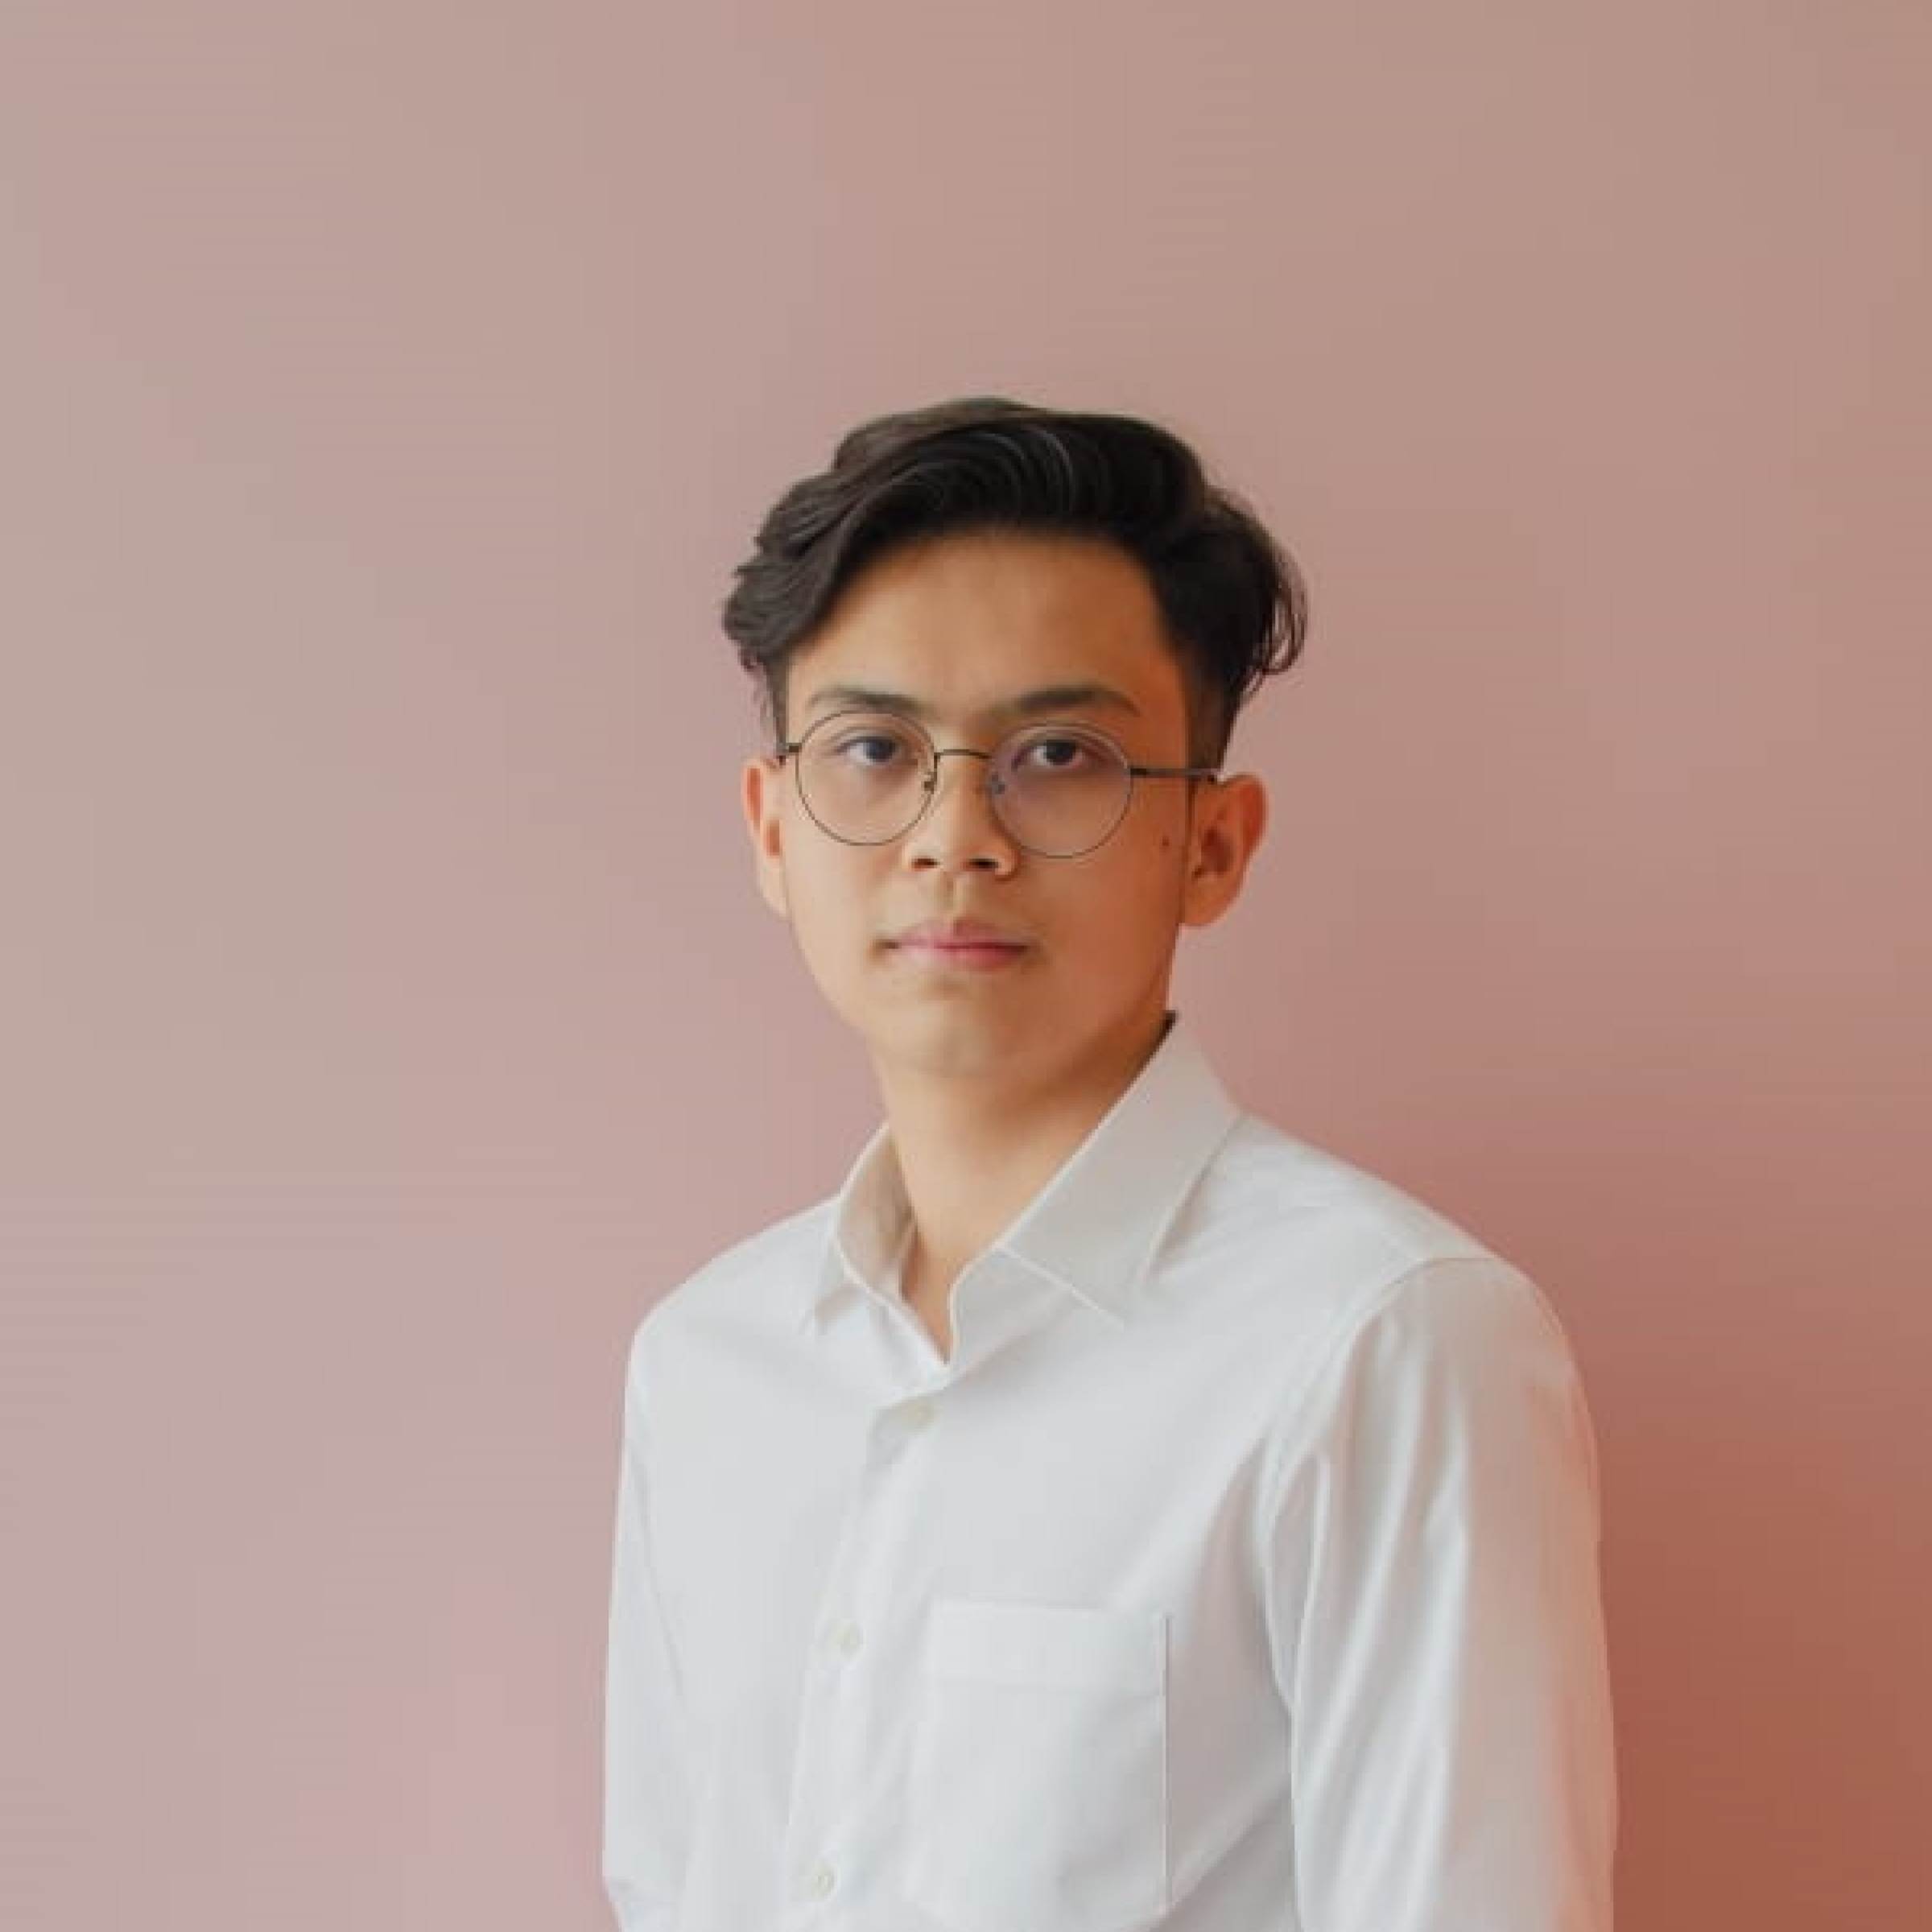
\includegraphics[width=0.3\textwidth]{gambar/foto-formal.png}
  \vspace{-4ex}
\end{wrapfigure}

% Ubah kalimat berikut dengan biografi dari mahasiswa
\name{}, atau yang biasa dikenal sebagai Krisna, lahir di Gianyar, Bali pada 8 Juli 2002. Penulis merupakan anak pertama dari tiga bersaudara yang tinggal dan tumbuh besar di Kota Denpasar, Bali. Ketertarikan mendalam penulis di bidang teknologi mengantarkan penulis yang telah menyelesaikan masa sekolah di SMA Negeri 4 Denpasar ke jenjang strata satu di Departemen Teknik Komputer Fakultas Teknologi Elektro dan Informatika Cerdas Institut Teknologi Sepuluh Nopember (ITS) pada tahun 2020.

Penulis merupakan pribadi yang memiliki ketertarikan dalam menjelajahi topik - topik yang berkaitan dengan bidang teknologi secara tekun dan mendalam. Dalam masa kuliah, penulis tertarik dengan topik seperti \emph{Internet Of Things} (IOT), Pengembangan Aplikasi (\emph{Mobile Development}), \emph{Machine Learning}, dan \emph{Computer Vision}. Penulis juga aktif dalam mengembangkan minat dan bakat di luar perkuliahan. Hal ini dibuktikan dengan rekam jejak organisasi dan kepanitian dari penulis seperti Wakil Ketua I Multimedia and Game Development (MAGE) 8, Koordinator Asisten Laboratorium Multimedia dan \emph{Internet Of Things} (IOT), hingga mengikuti program Bangkit Academy 2023. Hingga saat ini penulis terus menekani ketertarikan dan kemampuan yang dimiliki di bidang teknologi, terkhususnya pada bidang Pengembangan Aplikasi (\emph{Mobile Development}) dan \emph{Computer Vision}.

Pada penelitian tugas akhir ini, penulis memilih mengembangkan sistem penerjemah bahasa isyarat Indonesia (BISINDO) yang berfokus pada bidang \emph{Computer Vision}. Keresahan penulis yang memiliki suadara perempuan yang mengalami keterbatasan pendengaran dan berkomunikasi dengan bahasa isyarat menginspirasi dibuatnya tugas akhir ini sebagai bentuk upaya dalam memudahkan komunikasi teman tuli dengan khalayak umum. Bagi pembaca yang memiliki kritik, saran, atau pertanyaan mengenai tugas akhri ini dapat menghubungi penulis melalui surel krisnaerlangga08@gmail.com.

% \cleardoublepage

\end{document}
